\documentclass{osudissert96}
%
% To change the dissertation to a Master's Thesis, include a documentclass
% option such as [masters], [ms], [ma], etc.  Also available are [osudraft]
% and [twoside].  As a reminder, documentclass options are a
% comma-separated list, e.g. \documentclass[ms,osudraft]{osudissert96}

% Everything between the \documentclass and the \begin{document} is
% called the preamble of the document. Everything between the
% \begin{document} and the \end{document} is called the body of the
% document. Define any additional commands you want here (the preamble)

% BibTeX from the BiBTeX Documentation
\def\BibTeX{{\rm B\kern-.05em{\sc i\kern-.025em b}\kern-.08em
    T\kern-.1667em\lower.7ex\hbox{E}\kern-.125emX}}

%
% It is better to break up the dissertation into multiple files (e.g.,
% one file per chapter, as well as separate files for the abstract,
% acknowledgements, and vita).  These files are brought into the
% document using \include{} statements.  There will be times, however,
% when you don't want to print the ENTIRE dissertation.  You can limit
% what will actually be printed by using the \includeonly{} statement.
% This contains a list of the files you want printed.  Any file NOT
% listed will not be printed.  However, all page numbers, references,
% etc., will be preserved as though all the files were actually
% printed. For example, the line below would result only in chapters 1
% and 3 being printed (if it were uncommented).
%

%\includeonly{chapter-01-intro}

% UPDATED TEXT (2010):
%  In the newest format, titles should be title case everywhere.
%
% HISTORICAL TEXT (1996):
%  In the new format, the titles of each chapter should appear in
%  uppercase.  In the TOC, however, they should be in lowercase.
%  The command below automates this behavior.  However, you'll have to be
%  careful not to include \labels within your \chapter definitions or
%  there will be problems.  If you don't want this to be automated, comment
%  out the \typesetChapterTitle definition below and do your chapters in
%  the form:
%  \chapter[MY TITLE]{My Title}
%
%  \renewcommand\typesetChapterTitle[1]{\uppercase{#1}}
\renewcommand\typesetChapterTitle[1]{#1}

\begin{document}

%
% First, declare the parts of your title page 
%

\author{Chenxi Zhou}
\title{Density Estimation in Kernel Exponential Families: \\ Methods and Their Sensitivities}

\authordegrees{B.S.}  % Degrees thus far, not including this one.
\unit{Statistics}

\advisorname{Vincent Q. Vu}
\member{Yoonkyung Lee}
\member{Sebastian A. Kurtek}
%\member{Yet another dude}      % Normally you will have advisor + 2 members


%
% The following creates the title page
%

\maketitle

% Next, EITHER a copyright or BLANK page.
%
%   The following creates a page used to copyright your dissertation
%
%   BACKGROUND: Even without this copyright page, your dissertation will
%               carry a common-law copyright. However, if your
%               dissertation ends up seeing wide distribution, your
%               common-law copyright is at risk of being expunged.
%               Adding this copyright page prevents that from happening.
%
%               There are NO DOWNSIDES to including a copyright page as
%               your document is automatically copyright by law anyway.
%               However, this copyright page is OPTIONAL. If you get rid
%               of it, uncomment the \blankpage that follows it so that
%               there is a blank page here. The graduate school requires
%               a page here that is either blank or carries the
%               copyright.
%
%   IMPORTANT NOTE: The graduate school requires either a copyright page
%                   here or a BLANK PAGE here. If you get rid of the
%                   copyright, uncomment the \blankpage that follows it.
%                   You should NOT have BOTH uncommented.
%

% If you get rid of \disscopyright, restore the \blankpage line after it
\disscopyright
%\blankpage

%
% Abstract goes here.
%

\begin{abstract}
  %  The dissertation abstract can only be 500 words.

This dissertation is concerned with the nonparametric density estimation problem in a kernel exponential family, which is an exponential family induced by a reproducing kernel Hilbert space (RKHS). The corresponding density estimation problem can be formulated as a convex minimization problem over a RKHS or a subset of it. The loss functionals we focus on are the negative log-likelihood (NLL) loss functional and the score matching (SM) loss functional. 

We propose a new density estimator called the early stopping SM density estimator, which is obtained by applying the gradient descent algorithm to minimizing the SM loss functional and terminating the algorithm early to regularize. We investigate various statistical properties of this density estimator. We also compare this early stopping SM density estimator with the penalized SM density estimator that has been studied in the literature and address their similarities and differences. 

In addition, we propose an algorithm to compute the penalized maximum likelihood (ML) density estimator that is obtained by minimizing the penalized NLL loss functional. We empirically compare the penalized and early stopping SM density estimators with the penalized ML density estimator and find out that when there is a small amount of regularization (corresponding to small values of the penalty parameter or large values of the number of iterations), the regularized SM density estimates contain a bump or become a spike at the isolated observation, but the penalized ML density estimates do not. Moreover, if we remove the isolated observation, the resulting regularized SM density estimates do not contain a bump or a spike when the regularization is small. We attempt to explain why this happens. 

Observations above motivate us to study the sensitivities of different density estimators to the presence of an additional observation. We extend the definition of the influence function by allowing its input to be function-valued statistical functionals. We study various properties of this extended influence functions of ML and SM density projections in finite-dimensional and kernel exponential families, and empirically demonstrate that regularized SM density estimators in a kernel exponential family are more sensitive to the presence of an additional observation than the penalized ML density estimator when the amount of regularization is small. 

\end{abstract}


%
% UPDATED TEXT (2010):
%  The graduate school does not require an external abstract. If this
%  changes, follow the old instructions below.
%
% HISTORICAL TEXT (1996):
%  Uncomment the three lines below to generate the external abstract.  Two
%  copies of this must be turned in to the graduate school.  These lines can
%  be placed pretty much anywhere, since the page numbering should be
%  independent of the rest of the thesis
%

% \begin{externalabstract}
%   %  The dissertation abstract can only be 500 words.

This dissertation is concerned with the nonparametric density estimation problem in a kernel exponential family, which is an exponential family induced by a reproducing kernel Hilbert space (RKHS). The corresponding density estimation problem can be formulated as a convex minimization problem over a RKHS or a subset of it. The loss functionals we focus on are the negative log-likelihood (NLL) loss functional and the score matching (SM) loss functional. 

We propose a new density estimator called the early stopping SM density estimator, which is obtained by applying the gradient descent algorithm to minimizing the SM loss functional and terminating the algorithm early to regularize. We investigate various statistical properties of this density estimator. We also compare this early stopping SM density estimator with the penalized SM density estimator that has been studied in the literature and address their similarities and differences. 

In addition, we propose an algorithm to compute the penalized maximum likelihood (ML) density estimator that is obtained by minimizing the penalized NLL loss functional. We empirically compare the penalized and early stopping SM density estimators with the penalized ML density estimator and find out that when there is a small amount of regularization (corresponding to small values of the penalty parameter or large values of the number of iterations), the regularized SM density estimates contain a bump or become a spike at the isolated observation, but the penalized ML density estimates do not. Moreover, if we remove the isolated observation, the resulting regularized SM density estimates do not contain a bump or a spike when the regularization is small. We attempt to explain why this happens. 

Observations above motivate us to study the sensitivities of different density estimators to the presence of an additional observation. We extend the definition of the influence function by allowing its input to be function-valued statistical functionals. We study various properties of this extended influence functions of ML and SM density projections in finite-dimensional and kernel exponential families, and empirically demonstrate that regularized SM density estimators in a kernel exponential family are more sensitive to the presence of an additional observation than the penalized ML density estimator when the amount of regularization is small. 

% \end{externalabstract}

%
%  My Dedication
%

\dedication{To my family}

%
% Bring in Acknowledgement and Vita from separate files named ``ack.tex''
% and ``vita.tex''.
%

\begin{acknowledgements}


This dissertation would not have been possible without the help and support from many people. I would like to take this opportunity to express my sincerest gratitude. 

First, I would like to thank Dr. Vincent Vu, a great advisor for my academic research and a wonderful mentor for my life. His insightful questions and valuable guidance are always challenging my mind and pushing me to the next level. I am always grateful for his efforts and patience in training me to become a better critical thinker and problem solver. Additionally, I really appreciate his financial support during the summer terms. 

I would like to thank Dr. Yoonkyung Lee and Dr. Sebastian Kurtek for serving on my candidacy exam committee and dissertation committee, asking enlightening questions, and providing constructive suggestions and comments. I would also like to thank Dr. Subhadeep Paul for serving on my candidacy exam committee. I would also like to thank Dr. Radu Herbei for writing the recommendation letter for my PhD program application. 

I would like to thank many other professors in the Department of Statistics at The Ohio State University: Dr. Lo-Bin Chang, Dr. Peter Craigmile, Dr. Doug Critchlow, Dr. Steve MacEachern, Dr. Omer Ozturk, Dr. Xinyi Xu, and Dr. Yunzhang Zhu. It is my great honor to attend their courses and exchange ideas with them. Their expertise, knowledge and mindsets guided me through my PhD studies. 

Special thanks to the Nationwide Center for Advanced Customer Insights (NCACI) and Nationwide Mutual Insurance Company for the great opportunity to work as a Graduate Research Associate and the financial support of my graduate studies. It has been an amazing experience working  with these fantastic people there: Bob Forrest, Jonathon Huber, Craig Mass, Shannon Terry, David Weiner, Tim Welch, James Xia, Aimee Yoon, and Weiyan Zhao. Thank you all for always showing utmost confidence in me and guiding me so positively. 

My thanks also goes to Manisha Udhnani and Kate Valerio,  my therapists at the Psychological Services Center at The Ohio State University. Without your moral support and encouragement, I would not have been able to complete my research. 

I owe many friends a great debt of gratitude. Many thanks to Zifeng Cheng, Miaolai Han, Binshen He, Yujia Liu, Xincheng Shen, Yixing Shen, Min Shi, Wenzhe Sun, Minyu Wu, Ziyi Yang, Pengyi Ye, Runtian Zhang, and Qinwen Zhang. Without your enduring help, support, and encouragement, I would not have gone this far. 

Lastly, I would extend my gratitude to my parents, Jiangang Zhou and Ailing Chen, who brought me up with unconditional love, support and encouragement. 

Thank you everyone for being here with me along this journey. 

This dissertation is supported in part by the National Science Foundation under grants DMS-1513621 and DMS-1916446. 

\end{acknowledgements}

\begin{vita}

\dateitem{May 2015}{B.S. Mathematics and Economics with Honors, The Ohio State University}

\vspace{5pt}

\dateitem{August 2015 --- May 2019}{Graduate Teaching and Research Associate, Department of Statistics, The Ohio State University}

\vspace{10pt}

\dateitem{August 2019 --- present}{Graduate Research Associate, Nationwide Center for Advanced Customer Insights, Fisher College of Business, The Ohio State University}

%\begin{publist}

%% UPDATE FOR 2010:
%  Grad school only wants research publications, and it only wants those
%  research pubs that are actually published. Accepted or ``to appear''
%  publications don't count. If they look closely, they'll tell you to
%  remove any publications that aren't in print. Haivng said that, they
%  probably won't look that closely unless you put a really long list
%  here. You're tempting fate if you add instructional publications
%  though.

%\researchpubs
%
%\pubitem{B.~Simpson
%\newblock ``Milking a Cow''.
%\newblock {\em Journal of Dairy Science}, 00(2):277--287, Feb. 1900.}

% \instructpubs
%
% \pubitem{B.~Simpson, ed.,
% \newblock ``Lab notes for Cow Science 101'', 1909.}

%\end{publist}

\vspace{30pt}

\begin{fieldsstudy}

% The \majorfield* uses the unit specified in the \unit command used
% earlier in your document. If you want to use a different unit, use the
% second form shown here
% \majorfield*
\majorfield{Statistics}

%%
%% Note:  If there were only one field of study, the following list 
%%        would best be done using the following command:
%%
%%  \onestudy{Only Topic}{Only Professor}
%%

% \begin{studieslist}
% \studyitem{Topic 1}{Prof.\ Big Dude}
% \studyitem{Topic 2}{Prof.\ Other Dude}
% \studyitem{Topic 3}{Prof.\ Another Dude}
% \end{studieslist}

\end{fieldsstudy}

\end{vita}




%
% Make the Table of Contents and other good stuff
%

\tableofcontents
%\listoftables
\listoffigures

%\phantomsection \label{listofalgorithms}
%\addcontentsline{toc}{chapter}{List of Algorithms}
%\renewcommand{\listalgorithmname}{List of Algorithms}
%\listofalgorithms


%
% The following is a list of chapters.  Each is brought in from a
% separate file using the \include{} command.
%

\include{chapter-01-intro}

\include{chapter-02-kernel-exponential-family} 

\chapter{Early Stopping Score Matching Density Estimator}
\label{ch3}


In this chapter, we introduce the early stopping SM density estimator and discuss its statistical properties. As we have discussed in Chapter \ref{ch2}, minimizing $\widehat{J}_{\SM}$ over $\calH$ has no solution and a certain kind of regularization has to be imposed. The approach adopted by \textcite{Sriperumbudur-density-estimation-inf-exp-family} was to add a penalty functional and minimize the penalized SM loss functional, which yields the penalized SM density estimator. In this chapter, we consider the early stopping approach to regularize. More precisely, we apply the gradient descent algorithm to minimizing $\widehat{J}_{\SM}$ and terminate the algorithm early, leading to the early stopping SM density estimator. 

After an overview of the early stopping regularization and the gradient descent algorithm in Section \ref{section-gd-overview}, we present our early stopping SM density estimator in Section \ref{section-smes-estimator}. We then study its theoretical properties in Section \ref{section-theoretical-properties}. Finally, we compare our early stopping SM density estimator with the penalized SM density estimator in Section \ref{section-compare-smes-smpen}. 

\section{An Overview} \label{section-gd-overview}

Early stopping is a form of regularization based on choosing when to terminate an iterative optimization algorithm. This form of regularization is often referred to as implicit regularization, in contrast to the penalized approach by explicitly adding a penalty term. %The main advantage of early stopping regularization, compared with the penalized approach, is the lower computational complexity. 

In the supervised learning setting where a model is estimated via minimizing a loss function, using early stopping can effectively avoid overfitting so that the resulting estimated model can generalize well. It is essentially a bias-variance tradeoff: stopping the algorithm too early results in a model with a large bias and a small variance, but stopping it too late leads to a model with a small bias but a large variance. Stopping the algorithm early (but not too early) is an approach to solve this bias-variance tradeoff. Early stopping has been systematically investigated in $L_2$ boosting algorithm \parencite{Buhlmann2003-dk}, boosting algorithm for a general convex loss function \parencite{Zhang2005-pi}, and the nonparametric least squares regression in the RKHS setting \parencite{Yao2007-ji,Raskutti14-dw}, to name a few. 

In our development below, we choose the iterative optimization algorithm to be the gradient descent algorithm, which is a first-order optimization algorithm for solving an unconstrained minimization problem. Starting from a point in the feasible set, at each iteration, the gradient descent algorithm goes along the direction of the negative gradient of the objective function at the current point. This direction is the one with the steepest descent. 

Mathematically, let $g: \Real^m \to \Real$ be a convex differentiable function and assume there exists a unique $x^* \in \Real^m$ such that $\inf_{x \in \Real^m} g \parens{x} = g \parens{x^*} > -\infty$. We would like to minimize $g$ over $\Real^m$. Gradient descent algorithm starts from $x^{\parens{0}} \in \Real^m$ and generates the sequence 
\begin{align*}
	x^{\parens{t+1}} = x^{\parens{t}} - \tau_t \nabla g \parens{x^{\parens{t}}}, \qquad \qquad \text{ for all } t \in \Natural_0 := \Natural \cup \sets{0}, 
\end{align*}
where $\tau_t > 0$ is the appropriately chosen step size and the subscript ``$t$'' indicates that the step size may differ for different numbers of iterations. With appropriately chosen $\sets{\tau_t}_{t \in \Natural}$, the gradient descent algorithm guarantees $g$ is decreased at each iteration, i.e., $g \parens{x^{\parens{t+1}}} < g \parens{x^{\parens{t}}}$ for all $t \in \Natural_0$, except when $g$ has already achieved the minimum at $x^{\parens{t}}$. One terminates the algorithm when one of the following three criteria does not exceed a pre-specified tolerant parameter
\begin{align*}
	\norm{\nabla g \parens{x^{\parens{t}}}}, \qquad 
	\abs{g \parens{x^{\parens{t+1}}} - g \parens{x^{\parens{t}}}}, \qquad \text{ and } \qquad 
	\abs[\bigg]{\frac{g \parens{x^{\parens{t+1}}} - g \parens{x^{\parens{t}}}}{g \parens{x^{\parens{t}}}} }, 
\end{align*}
where $\norm{\,\cdot\,}$ is a norm over $\Real^m$ chosen by the user. It can be shown that, with appropriately chosen $\sets{\tau_t}_{t \in \Natural}$, the sequence $\sets{g \parens{x^{\parens{t}}}}_{t \in \Natural}$ is guaranteed to converge to $g \parens{x^*}$ as $t \to \infty$ \parencites[see, for example, Chapter 9 in][]{Boyd2004-gi}. 

%Gradient descent method has found a wide range of applications in statistical estimation. We provide one example here. 
%
%\begin{example}[Least Squares Regression]
%	In the least squares regression, we assume the response variable $Y \in \Real$ and the covariate $X \in \Real^d$ are related by the model 
%	\begin{align}
%		Y = X^\top \beta^* + \varepsilon, 
%	\end{align}
%	where $\beta^* \in \Real^d$ is the true coefficient and $\varepsilon \sim \Normal \parens{0, \sigma^2}$ with $\sigma^2 > 0$ being unknown. Let $\sets{\parens{Y_i, X_i}}_{i=1}^n$ are $n$ i.i.d observations, where we assume $n > d$. We estimate $\beta^* := \parens{\beta_1^*, \cdots, \beta_d^*}^\top \in \Real^d$ using the least squares method, which amounts to minimizing 
%	\begin{align}\label{eq-least-squares-regression}
%		\frac{1}{2} \norm{\bY - \bX \beta}_2^2, 
%	\end{align}
%	where $\bY := \parens{Y_1, \cdots, Y_n}^\top \in \Real^n$ and $\bX \in \Real^{n \times d}$ is the design matrix with each row corresponding to an observation and each column corresponding to a covariate. We assume that the matrix $\bX$ is of full rank. 
%	
%	The problem of minimizing \eqref{eq-least-squares-regression} has an analytic solution given by 
%	\begin{align}\label{eq-least-square-inverse}
%		\hat{\beta} := \parens{\bX^\top \bX}^{-1} \bX^\top \bY, 
%	\end{align}
%	where $\parens{\bX^\top \bX}^{-1}$ exists since $\bX$ has full rank. Note that to compute \eqref{eq-least-square-inverse} requires to compute $\parens{\bX^\top \bX}^{-1}$, which requires elementary operations of order $\calO \parens{p^3}$. If $p$ is large, the computation is expensive. 
%	
%	We could also minimize \eqref{eq-least-squares-regression} using the gradient descent algorithm. Starting from $\beta^{\parens{0}}$, the gradient descent iterates are given by 
%	\begin{align*}
%		\beta^{\parens{t+1}} = \beta^{\parens{t}} - \tau \bX^\top \parens{\bX \beta^{\parens{t}} - \bY}, \qquad \text{ for all } t \in \Natural_0 := \Natural \cup \sets{0}, 
%	\end{align*}
%	where $\tau > 0$ is the constant step size. We terminate the algorithm when $\norm{\bX^\top \parens{\bX \beta^{\parens{t}} - \bY}} \le \gamma$, where $\gamma > 0$ is a pre-specified positive constant. With an appropriate $\tau$, computing $\beta^{\parens{t}}$ only requires elementary operations of order $\calO \parens{p^2 n}$. From here, we see the computational advantage of using the gradient descent algorithm over working with the analytic solution directly using \eqref{eq-least-square-inverse}. 
%\end{example}

\section{Early Stopping Score Matching Density Estimator}\label{section-smes-estimator}

We present our early stopping SM density estimator in this section. %, which is obtained by applying the gradient descent algorithm to minimizing $\widehat{J}_{\SM}$ over $\calH$ and terminating the algorithm early. 

To start with, we formally state a set of assumptions, in addition to \ref{assumption-2-1-inf-dim} - \ref{assumption-2-4-base-density} in Chapter \ref{ch2}, that will be used. 

\begin{enumerate}[label=\textbf{(B\arabic*)},series=assumptions]
	\item \label{assumption-1} $\calX$ is a non-empty open subset of $\Real^d$ with a piecewise smooth boundary $\partial \calX := \overline{\calX} \backslash \calX$, where $\overline{\calX}$ denotes the closure of $\calX$. 
	\item \label{assumption-2} $p_0$ is continuously differentiable, is continuously extendible to $\overline{\calX}$, and satisfies $\int_{\calX} p_0 \parens{x} \norm{\nabla \log p_0 \parens{x}}_2^2 \diff x < \infty$. 
	\item \label{assumption-3} $k$ is twice continuously differentiable on $\calX \times \calX$ with continuous extension of $\partial_u \partial_{u+d} k$ and $\partial_u \partial_v \partial_{u+d} \partial_{v+d} k$ to $\overline{\calX} \times \overline{\calX}$ for all $u, v = 1, 2, \cdots, d$. 
	\item \label{assumption-4} As $x \to \partial \calX$, $\sup_{u = 1, \cdots, d} \partial_u \partial_{u+d} k \parens{x, x} p_0 \parens{x} \to 0$.  
	\item \label{assumption-5} $\kappa_2 := \sup_{u = 1, \cdots, d} \sup_{x \in \calX} \sqrt{\partial_u \partial_{u+d} k \parens{x, x}} < \infty$, \\ 
		$\kappa_3 := \sup_{u = 1, \cdots, d} \sup_{x \in \calX} \sqrt{\partial_u^2 \partial_{u+d}^2 k \parens{x, x}} < \infty$, and \\ 
		$\kappa_4 := \sup_{u = 1, \cdots, d} \sup_{x \in \calX} \abs{\partial_u \log \mu \parens{x}} \sqrt{\partial_u \partial_{u+d} k \parens{x, x}}  < \infty$. 
\end{enumerate}

Under these assumptions, we can derive the H-divergence between $p_0$ and $q_f \in \calQ_{\ker}$ and the corresponding SM matching loss that we have seen in Chapter \ref{ch2}. 

\begin{theorem}[Theorem 4 in \textcite{Sriperumbudur-density-estimation-inf-exp-family}]\label{thm-smloss} \leavevmode
\begin{enumerate}[label=(\alph*)]
	\item Under \ref{assumption-2-1-inf-dim} - \ref{assumption-2-4-base-density} in Chapter \ref{ch2} and \ref{assumption-1} - \ref{assumption-5} above, the H-divergence between $p_0$ and $q_f \in \calQ_{\kef}$ is 
	\begin{align*}
		J_{\SM} \parens{f} := \frac{1}{2} \innerp{f}{C f}_{\calH} - \innerp{f}{z}_{\calH} + \mathrm{const}, 
	\end{align*}
	where $C: \calH \to \calH$ is a linear positive semidefinite operator given by 
	\begin{align}\label{eq-C-def}
		C := \int_{\calX} p_0 \parens{x} \sum_{u=1}^d \partial_u k \parens{x, \,\cdot\,} \otimes \partial_u k \parens{x, \,\cdot\,} \diff x
	\end{align}
	satisfying $C f = \int_{\calX} p_0 \parens{x} \sum_{u=1}^d \partial_u f \parens{x} \partial_u k \parens{x, \,\cdot\,} \diff x$ for all $f \in \calH$, and $z: \calX \to \Real$ is a function in $\calH$ given by 
	\begin{align}\label{eq-z-def}
		z := - \int_{\calX} p_0 \parens{x} \sum_{u=1}^d \parens[\Big]{\partial^2_u k \parens{x, \,\cdot\,} + \partial_u \log \mu \parens{x} \partial_u k \parens{x, \,\cdot\,}} \diff x, 
	\end{align}
	and const is a term that does \emph{not} depend on $f$ and is equal to $\frac{1}{2} \int_{\calX} p_0 \parens{x} \norm[\big]{\nabla \log p_0 \parens{x} - \nabla \log \mu \parens{x}}_2^2 \diff x$. 
	
	\item Let $X_1, \cdots, X_n$ be i.i.d samples from $p_0$. Under \ref{assumption-2-1-inf-dim} - \ref{assumption-2-4-base-density} in Chapter \ref{ch2}, \ref{assumption-1} - \ref{assumption-5} above, and $q_f \in \calQ_{\kef}$, the SM loss functional is $\widehat{J}_{\SM}: \calH \to \Real$ given by 
	\begin{equation*}% \label{eq-smloss}
		\widehat{J}_{\SM} \parens{f} := \frac{1}{2} \langle f, \widehat{C} f \rangle_{\mathcal{H}} - \langle f, \hat{z} \rangle_{\mathcal{H}} + \mathrm{const}, \qquad \text{ for all } f \in \calH, 
	\end{equation*}
	where $\widehat{C}: \calH \to \calH$ and $\hat{z} \in \calH$ are given by \eqref{eq-hatC} and \eqref{eq-hatz} in Chapter \ref{ch2}, respectively.  
%	\begin{align}\label{eq-hatC-def}
%		\widehat{C} := \frac{1}{n} \sum_{i=1}^n \sum_{u=1}^d \partial_u k \parens{X_i, \,\cdot\,} \otimes \partial_u k \parens{X_i, \,\cdot\,}
%	\end{align}
%	with
%	\begin{align}
%		\widehat{C} f =  \frac{1}{n} \sum_{i=1}^n \sum_{u=1}^d \partial_u f \parens{X_i} \partial_u k \parens{X_i, \,\cdot\,} \quad \text{ for all } f \in \calF, 
%	\end{align}
%	and 
%	\begin{align}\label{hatz.def}
%		\hat{z} := -\frac{1}{n} \sum_{i=1}^n \sum_{u=1}^d \parens[\Big]{\partial^2_u k \parens{X_i, \,\cdot\,} + \partial_u \log \mu \parens{X_i} \partial_u k \parens{X_i, \,\cdot\,}} \in \calH, 
%	\end{align}
%	and const is given by \eqref{eq-T-term} and does not depend on $f$. 
\end{enumerate}
\end{theorem}

The proof of this theorem can be found in \textcite{Sriperumbudur-density-estimation-inf-exp-family} and is omitted here. 

%In order to prove Theorem \ref{thm-smloss}, we need the following lemma from \textcite{Zhou2008-jt}. 
%
%\begin{lemma}[Properties of partial derivatives of kernel function]\label{lemma-zhou-theorem}
%	Assume $k: \calX \times \calX \to \Real$ is twice continuously differentiable over $\calX$. Let $x \in \calX$ and $u \in \sets{1, \cdots, d}$. Then, 
%	\begin{enumerate}[label=(\alph*)]
%		\item both $\partial_u k \parens{x, \,\cdot\,}$ and $\partial_u^2 k \parens{x, \,\cdot\,}$ belong to $\calH$, and 
%		\item for any $f \in \calH$, 
%		\begin{align}
%		  \partial_u f \parens{x} = & \, \innerp{f}{\partial_u k \parens{x, \,\cdot\,}}_{\calH}, \qquad \text{ and } \qquad \partial_u^2 f \parens{x} = \innerp{f}{\partial_u^2 k \parens{x, \,\cdot\,}}_{\calH}, 
%		\end{align}
%		where $\partial_u f$ and $\partial_u^2 f$ denote the first- and second-order partial derivatives of $f$ with respect to the $u$-th coordinate, respectively. 
%	\end{enumerate}
%\end{lemma}
%
%Now, we are ready to prove Theorem \ref{thm-smloss}. 
%
%\begin{proof}[Proof of Theorem \ref{thm-smloss}]
%	(a) By the definition of the H-divergence, we have 
%	\begin{align}
%		\Hdiv \parens{p_0 \Vert q_f} := & \, \frac{1}{2} \int_{\calX} p_0 \parens{x} \norm[\big]{\nabla \log p_0 \parens{x} - \nabla \log q_f \parens{x}}_2^2 \diff x \nonumber \\
%		= & \, \frac{1}{2} \int_{\calX} p_0 (x) \parens[\Big]{\norm{\nabla \log q_f \parens{x}}_2^2 - 2 \innerp[\big]{\nabla \log p_0 \parens{x}}{\nabla \log q_f \parens{x}} + \norm{\nabla \log p_0 \parens{x}}_2^2} \diff x, \label{eq-29}
%	\end{align}
%	where $\nabla \log p \parens{x} := \parens[\big]{\partial_1 \log p \parens{x}, \cdots, \partial_d \log p \parens{x}}^\top \in \Real^d$ and $\partial_u \log p \parens{x} := \frac{\partial \log p \parens{w}}{\partial w_u} \Big\vert_{w = x}$ for $w = \parens{w_1, \cdots, w_d} \in \calX$ and all $u = 1, \cdots, d$. In \eqref{eq-29}, $\innerp{\,\cdot\,}{\,\cdot\,}$ denotes the usual dot product in $\Real^d$ and $\norm{\,\cdot\,}_2$ denotes the Euclidean norm in $\Real^d$. 
%	
%	First note that $\int_{\calX} p_0 \parens{x} \norm{\nabla \log p_0 \parens{x}}_2^2 \diff x$ does not depend on $f$ and is finite by \ref{assumption-2}. 
%	
%	Since $\nabla \log q_f \parens{x} = \nabla \log \mu \parens{x} + \nabla f \parens{x}$, we have 
%	\begin{align*}
%		  \int_{\calX} p_0 \parens{x} \norm[\big]{\nabla \log q_f \parens{x}}_2^2 \diff x 
%		% = & \, \int_{\calX} p_0 \parens{x} \sum_{u=1}^d \parens[\big]{\partial_u \log \mu \parens{x} + \partial_u f \parens{x}}^2 \diff x \\ 
%		= & \, \int_{\calX} p_0 \parens{x} \sum_{u=1}^d \parens[\big]{\partial_u \log \mu \parens{x}}^2 \diff x + 2 \int_{\calX} p_0 \parens{x} \sum_{u=1}^d \partial_u \log \mu \parens{x} \partial_u f \parens{x} \diff x \\ 
%		  & \qquad \qquad + \int_{\calX} p_0 \parens{x} \sum_{u=1}^d \parens[\big]{\partial_u f \parens{x}}^2 \diff x \\
%		\stackrel{\text{(i)}}{=} & \, \int_{\calX} p_0 \parens{x} \norm[\big]{\nabla \log \mu \parens{x}}_2^2 \diff x  + 2 \int_{\calX} p_0 \parens{x} \sum_{u=1}^d \partial_u \log \mu \parens{x} \innerp{f}{\partial_u k \parens{x, \cdot}}_{\calH} \diff x \\ 
%		  & \qquad + \int_{\calX} p_0 \parens{x} \sum_{u=1}^d \innerp[\big]{f}{\parens[\big]{\partial_u k \parens{x, \cdot} \otimes \partial_u k \parens{x, \cdot}} f}_{\calH} \diff x, \\
%		\stackrel{\text{(ii)}}{=} & \, \int_{\calX} p_0 \parens{x} \norm[\big]{\nabla \log \mu \parens{x}}_2^2 \diff x + \innerp[\bigg]{f}{2 \int_{\calX} p_0 \parens{x} \sum_{u=1}^d \partial_u \log \mu \parens{x} \partial_u k \parens{x, \cdot} \diff x}_{\calH} \\ 
%		  & \qquad + \innerp[\bigg]{f}{\parens[\bigg]{\int_{\calX} p_0 \parens{x} \sum_{u=1}^d \partial_u k \parens{x, \cdot} \otimes \partial_u k \parens{x, \cdot} \diff x} f}_{\calH}, 
%	\end{align*}
%	where we use Lemma \ref{lemma-zhou-theorem} and $\innerp{a}{b}_{\calH}^2 = \innerp{a}{b}_{\calH} \innerp{a}{b}_{\calH} = \innerp{a}{\parens{b \otimes b} a}_{\calH}$, for $a, b \in \calH$, in (i), and swap the integral and the inner product in (ii) using \ref{assumption-6}. 
%	
%	As for $\int_{\calX} p_0 \parens{x} \innerp{\nabla \log p_0 \parens{x}}{\nabla \log q_f \parens{x}} \diff x$ in \eqref{eq-29}, we have 
%	\begin{align*}
%		& \, \int_{\calX} p_0 \parens{x} \innerp[\big]{\nabla \log p_0 \parens{x}}{\nabla \log q_f \parens{x}} \diff x \\ 
%		= & \, \int_{\calX} p_0 \parens{x} \innerp[\big]{\nabla \log p_0 \parens{x}}{\nabla \log \mu \parens{x}} \diff x + \sum_{u=1}^d \int_{\calX} p_0 \parens{x} \frac{\partial_u p_0 \parens{x}}{p_0 \parens{x}} \partial_u f \parens{x} \diff x \\ 
%	 	= & \, \int_{\calX} p_0 \parens{x} \innerp[\big]{\nabla \log p_0 \parens{x}}{\nabla \log \mu \parens{x}} \diff x + \sum_{u=1}^d \int_{\calX} \partial_u p_0 \parens{x} \partial_u f \parens{x} \diff x \\ 
%		\stackrel{\text{(iii)}}{=} & \, \int_{\calX} p_0 \parens{x} \innerp[\big]{\nabla \log p_0 \parens{x}}{\nabla \log \mu \parens{x}} \diff x - \sum_{u=1}^d \int_{\calX} p_0 \parens{x} \partial_u^2 f \parens{x} \diff x \\
%		\stackrel{\text{(iv)}}{=} & \, \int_{\calX} p_0 \parens{x} \innerp[\big]{\nabla \log p_0 \parens{x}}{\nabla \log \mu \parens{x}} \diff x - \innerp[\bigg]{f}{\int_{\calX} p_0 \parens{x} \sum_{u=1}^d \partial_u^2 k \parens{x, \cdot} \diff x}_{\calH}, 
%	\end{align*}
%	where (iii) is due to the integration by parts and \ref{assumption-5} and (iv) is due to Lemma \ref{lemma-zhou-theorem} and \ref{assumption-6}. 
%	
%	Putting things together, we have 
%	\begin{align*}
%		\Hdiv \parens{p_0 \Vert q_f} = & \, \frac{1}{2} \innerp[\bigg]{f}{\parens[\bigg]{\int_{\calX} p_0 \parens{x} \sum_{u=1}^d \partial_u k \parens{x, \cdot} \otimes \partial_u k \parens{x, \cdot} \diff x} f}_{\calH} \\ & \, - \innerp[\bigg]{f}{- \int_{\calX} p_0 \parens{x} \sum_{u=1}^d \parens[\big]{\partial_u \log \mu \parens{x} \partial_u k \parens{x, \cdot} + \partial_u^2 k \parens{x, \cdot}} \diff x}_{\calH} \\ 
%		& \qquad + \frac{1}{2} \int_{\calX} p_0 \parens{x} \parens[\Big]{ \norm{\nabla \log p_0 \parens{x}}_2^2 - 2 \innerp{\nabla \log p_0 \parens{x}}{\nabla \log \mu \parens{x}} \norm{\log \mu \parens{x}}_2^2} \diff x \\ 
%	  = & \, \frac{1}{2} \innerp[\big]{f}{C f}_{\calH} - \innerp[\big]{f}{z}_{\calH} + const. 
%	\end{align*}
%	
%	(b) In order to obtain $\widehat{J}$ as in \eqref{eq-smloss}, simply replace the integrals in $C$ and $z$ by their sample counterparts using $X_1, \cdots, X_n \stackrel{\text{i.i.d}}{\sim} p_0$. 
%\end{proof}

As we have discussed in Section \ref{subsection-sm-kef} in Chapter \ref{ch2}, minimizing $\widehat{J}_{\SM}$ over $\calH$ does \emph{not} have a solution. In order to obtain a solution, we need to impose certain kind of regularization. We apply the gradient descent algorithm to minimizing $\widehat{J}_{\SM}$ and terminate it early to regularize. Since $\widehat{J}_{\SM}$ maps from $\calH$ to $\Real$, we need a notion of the gradient defined for functionals whose input space is a Hilbert space. We again use the Fr{\'e}chet gradient (see Definition \ref{def-frechet-gradient} in Appendix \ref{app1}) and derive the Fr{\'e}chet gradient of $\widehat{J}_{\SM}$ in the following theorem. 

\begin{theorem}[Fr{\'e}chet gradient of $\widehat{J}_{\SM}$]\label{thm-grad-widehatJ}
	Under the same assumptions in Theorem \ref{thm-smloss}, the Fr{\'e}chet gradient of $\widehat{J}_{\SM}$, denoted by $\nabla \widehat{J}_{\SM}$, is a map from $\calH$ to $\calH$ given by 
	\begin{align*}
		\nabla \widehat{J}_{\SM} \parens{f} = \widehat{C} f - \hat{z}, \qquad \qquad \text{ for all } f \in \calH. 
	\end{align*}
\end{theorem}

The proof of Theorem \ref{thm-grad-widehatJ} can be found in Section \ref{proof-thm-grad-widehatJ}. 

With the result of Theorem \ref{thm-grad-widehatJ}, starting from some $\hat{f}_{\SM}^{\parens{0}} \in \calH$, the gradient descent iterates are 
\begin{align}
	\hat{f}_{\SM}^{\parens{t+1}} = & \, \hat{f}_{\SM}^{\parens{t}} - \tau_{t} \nabla \widehat{J}_{\SM} \parens{\hat{f}_{\SM}^{\parens{t}}} \nonumber \\ 
	= & \, \hat{f}_{\SM}^{\parens{t}} - \tau_{t} \parens{\widehat{C} \hat{f}_{\SM}^{\parens{t}} - \hat{z}}, \qquad \text{ for all } t \in \Natural_0, \label{eq-grad-updates}
\end{align}
where $\tau_t \in \parens{0, 1 / \parens{d \kappa_2^2} }$ is the step size at the $t$-th iterate. We omit the subscript ``SM'' associated with $\hat{f}_{\SM}^{\parens{t}}$ in the rest of this chapter for notational simplicity. 

Using the definition of the second-order Fr{\'e}chet derivative and gradient (Definition \ref{def-frechet-derivative-higher-order} in Appendix \ref{app1}), we know $\widehat{J}_{\SM}$ is twice Fr{\'e}chet differentiable and $\nabla^2 \widehat{J}_{\SM} \parens{f} = \widehat{C}$, for all $f \in \calH$. Using \ref{assumption-5}, we have $\norm{\widehat{C}} \le d \kappa_2^2$, where $\norm{\widehat{C}}$ denotes the operator norm of $\widehat{C}$. By the standard results on the gradient descent algorithm, with the choice of $\tau_t \in \parens{0, 1 / \parens{d \kappa_2^2} }$, the value of $\widehat{J}_{\SM}$ is guaranteed to decrease at each iteration. 

The following theorem links $\hat{f}^{\parens{t+1}}$ to $\hat{f}^{\parens{0}}$ for an arbitrary $t \in \Natural_0$ and will help us derive a practical algorithm to compute $\hat{f}^{\parens{t+1}}$ and facilitate our analysis in Section \ref{section-theoretical-properties}. 

\begin{theorem}\label{thm-closed-form}
	Starting the gradient descent algorithm from $\hat{f}^{\parens{0}} \in \calH$, the $\parens{t+1}$-st gradient descent iterate is 
	\begin{align}\label{eq-closed-form}
		\hat{f}^{\parens{t+1}} = \prod_{i=0}^{t} \parens{I - \tau_i \widehat{C}} \hat{f}^{\parens{0}} + \sum_{j=0}^{t} \bracks[\Bigg]{\prod_{i=j+1}^{t} \parens{I - \tau_i \widehat{C}}} \tau_j \hat{z}, \qquad \text{ for all } t \in \Natural_0, 
	\end{align}
	where $I: \calH \to \calH$ is the identity operator, and $\prod_{i=t+1}^{t} \parens{I - \tau_i \widehat{C}} = I$ for all $t \in \Natural_0$. If, in particular, we choose the constant step size, that is, $\tau_t \equiv \tau$ for all $t \in \Natural_0$, we have
	\begin{align*}
		\hat{f}^{\parens{t+1}} = \parens{I - \tau \widehat{C}}^{t+1} \hat{f}^{\parens{0}} + \tau \sum_{j=0}^{t} \parens{I - \tau \widehat{C}}^{t-j} \hat{z}. 
	\end{align*}
	Here, $\parens{I - \tau \widehat{C}}^{i} \hat{z}$, for any $i \in \Natural_0$, is defined as 
	\begin{align*}
		\parens{I - \tau \widehat{C}}^{0} \hat{z} = & \, \hat{z}, \qquad \text{ and } \qquad
		\parens{I - \tau \widehat{C}}^{i} \hat{z} = \parens{I - \tau \widehat{C}} \bracks[\big]{\parens{I - \tau \widehat{C}}^{i-1} \hat{z}} \text{ for all } i \ge 1. 
	\end{align*}
\end{theorem}

The proof of Theorem \ref{thm-closed-form} can be found in Section \ref{proof-thm-closed-form}. 

In order to compute $\hat{f}^{\parens{t}}$, we have to choose $\hat{f}^{\parens{0}}$. Different choices of $\hat{f}^{\parens{0}}$ leads to different trajectories of gradient descent iterates and, hence, different density estimates. We choose $\hat{f}^{\parens{0}} = 0 \in \calH$ for two reasons. First, this choice makes the computation and the theoretical analysis in the sequel easier, since, with $\hat{f}^{\parens{0}} = 0$, we can ignore the term $\prod_{i=0}^{t} \parens{I - \tau_i \widehat{C}} \hat{f}^{\parens{0}}$, and \eqref{eq-closed-form} becomes 
\begin{align*}
	\hat{f}^{\parens{t+1}} = \sum_{j=0}^t \bracks[\Bigg]{\prod_{i=j+1}^t \parens{I - \tau_i \widehat{C}}} \tau_j \hat{z}. 
\end{align*}
Second, this choice makes the early stopping and penalized SM density estimators comparable. In the penalized approach, the penalty term $\frac{1}{2} \norm{f}_{\calH}^2$ shrinks the natural parameter toward the zero function, and, as the penalty parameter $\rho \to \infty$, $q_{\hat{f}_{\SM}^{\parens{\rho}}} \to \mu$. In the early stopping approach, with $\hat{f}^{\parens{0}} = 0$, we have $q_{\hat{f}^{\parens{0}}} = \mu$, corresponding to the case $\rho \to \infty$ in the penalized approach. As the gradient descent algorithm evolves, the resulting early stopping SM density estimates correspond to the penalized ones with smaller $\rho$ values. % We will make the similarities between these two kinds of regularized SM density estimates more apparent in Section \ref{section-compare-smes-smpen}. 

\subsection{Computation}

Even though Theorem \ref{thm-closed-form} is useful in characterizing $\hat{f}^{\parens{t}}$ for each $t \in \Natural_0$ and in the subsequent analysis, it is not very directly applicable to produce an implementable algorithm to compute $\hat{f}^{\parens{t}}$, since \eqref{eq-closed-form} involves $\widehat{C}$ and $\hat{z}$ that reside in an infinite-dimensional RKHS. With the choice of $\hat{f}^{\parens{0}} = 0 \in \calH$, our goal of this section is to derive practical algorithms to compute $\hat{f}^{\parens{t}}$ for each $t \in \Natural$. 

\subsubsection{The First Algorithm}\label{subsection-first-algorithm}

	Note that, with $\hat{f}^{\parens{0}} = 0$, gradient descent iterates 
	\begin{align*}
		\hat{f}^{\parens{t+1}} = \hat{f}^{\parens{t}} - \tau \parens{\widehat{C} \hat{f}^{\parens{t}} - \hat{z}}
	\end{align*}
	belong to the union of $\range \parens{\widehat{C}}$ and $\sets{z}$. Since, for an arbitrary $g \in \calH$, $\widehat{C} g = \frac{1}{n} \sum_{i=1}^n \sum_{u=1}^d \innerp{g}{\partial_u k \parens{X_i, \,\cdot\,}}_{\calH} \partial_u k \parens{X_i, \,\cdot\,}$, we have 
	\begin{align*}% \label{eq-range-hatC}
		\range \parens{\widehat{C}} 
%		= & \, \sets{f \in \calH: f = Cg \text{ for some } g \in \calH} \\ 
%		= & \, \sets[\bigg]{f \in \calH: f = \frac{1}{n} \sum_{a=1}^n \sum_{i=1}^d \partial_i g(X_a) \partial_i k(X_a, \cdot) \text{ for some } g \in \calH} \\ 
		= & \, \text{Span} \sets[\Big]{\partial_u k \parens{X_i, \,\cdot\,}, \text{ for all } i = 1, \cdots, n, \text{ and } u = 1, \cdots, d}. 
	\end{align*}
	Therefore, the gradient descent iterates, $\hat{f}^{\parens{t+1}}$ for all $t \in \Natural_0$, must lie in the linear subspace 
	\begin{align}\label{eq-basis-func}
		\text{Span} \braces[\Big]{\partial_u k \parens{X_i, \,\cdot\,} \text{ for all } i = 1, \cdots, n \text{ and } u = 1, \cdots, d, \hat{z}}, 
	\end{align}
	which is of the dimensionality (at most) $nd + 1$. 
	% In particular, this indicates that the gradient descent iterates can be represented as linear combinations of basis functions $\partial_u k \parens{X_i, \,\cdot\,}$ for all $i = 1, \cdots, n$ and $u = 1, \cdots, d$, and $\hat{z}$. 
	% Since any finite dimensional vector space is isomorphic to the Euclidean space of the same dimensionality, we can, by a change of basis, re-express the solution as a linear combination of $\partial_i k(X_a, \cdot)$ for $a = 1, \cdots, n$ and $i = 1, \cdots, d$ and $\hat{\xi}$. 
	
	Since any $\tilde{f}$ belonging to \eqref{eq-basis-func} can be written as 
	\begin{align}\label{eq-solform}
		\tilde{f} = & \, \sum_{j=1}^n \sum_{v=1}^d \beta_{\parens{j-1}d+v} \partial_v k \parens{X_j, \,\cdot\,} + \beta_{nd+1} \hat{z}, 
	\end{align}
	plugging \eqref{eq-solform} into $\widehat{J}_{\SM}$ yields 
	\begin{align*}
		\widetilde{J}_{\SM} \parens{\bbeta} := \widehat{J}_{\SM} \parens{\tilde{f}} 
		= & \, \frac{1}{2n} \bbeta^\top \widetilde{\bG}^\top \widetilde{\bG} \bbeta - \bbeta^\top \widetilde{\bh}, 
	\end{align*}
	where $\bbeta := \parens{\beta_{1}, \cdots, \beta_{nd}, \beta_{nd+1}}^\top \in \Real^{nd+1}$, and 
	\begin{align*}
		\widetilde{\bG} := \bracks[\Big]{ \
			\bG \  \vdots \  \bh \ } \in \Real^{nd \times \parens{nd+1}}, \qquad \text{ and } \qquad \widetilde{\bh} := \bracks[\Big]{ \bh^\top \ \vdots \ \norm{\hat{z}}_{\calH}^2 }^\top \in \Real^{(nd+1) \times 1}. 
	\end{align*}
	
%	\begin{align*}
%		\widetilde{J} \parens{\bbeta} := & \, \frac{1}{2n} \sum_{i=1}^n \sum_{u=1}^d \parens[\bigg]{\innerp[\bigg]{\sum_{j=1}^n \sum_{v=1}^d \beta_{\parens{b-1}d+j} \partial_v k \parens{X_j, \,\cdot\,} + \beta_{nd+1} \hat{z}}{\partial_i k \parens{X_i, \,\cdot\,}}_{\calH}}^2 - \\ 
%		& \qquad \quad \innerp[\bigg]{\sum_{b=1}^n \sum_{j=1}^d \beta_{\parens{j-1} d+v} \partial_v k \parens{X_j, \,\cdot\,} + c_{nd+1} \hat{z}}{\hat{z}}_{\calH} \\ 
%		= & \, \frac{1}{2n} \sum_{i=1}^n \sum_{u=1}^d \Bigg[ \sum_{j=1}^n \sum_{v=1}^d \beta_{\parens{j-1}d+v} \partial_u \partial_{v+d} k \parens{X_i, X_j} + \beta_{nd+1} \innerp{\hat{z}}{\partial_u k \parens{X_i, \,\cdot\,}}_{\calH} \Bigg]^2 - \\ 
%		  & \qquad \parens[\bigg]{\sum_{j=1}^n \sum_{v=1}^d \beta_{\parens{j-1}d+v} \innerp{\partial_v k \parens{X_j, \cdot}}{\hat{z}}_{\calH} + \beta_{nd+1} \norm{\hat{z}}_{\calH}^2}. 
%	\end{align*}
%	We now rewrite $\widetilde{J} \parens{\bbeta}$ in the vector-matrix form. With the matrices $\bG \in \Real^{nd \times nd}$ and $\bh \in \Real^{nd}$ defined in Theorem \ref{thm-early-stopping-algo}, construct 
%	\begin{align*}
%		\widetilde{\bG} := \bracks[\Big]{ \
%			\bG \  \vdots \  \bh \ } \in \Real^{nd \times \parens{nd+1}}, \qquad \text{ and } \qquad \widetilde{\bh} := \bracks[\Big]{ \bh^\top \ \vdots \ \norm{\hat{z}}_{\calH}^2 }^\top \in \Real^{(nd+1) \times 1}. 
%	\end{align*}
%	Then, we can write $\widetilde{J} \parens{\bbeta}$ as 
%	\begin{align}
%		\widetilde{J} \parens{\bbeta} = & \, \frac{1}{2n} \sum_{i=1}^n \sum_{u=1}^d \parens[\big]{\bbeta^\top \widetilde{\bG} \parens{\parens{i - 1} d+u}}^2 - \bbeta^\top \widetilde{\bh} \nonumber \\ 
%		= & \, \frac{1}{2n} \sum_{a=1}^n \sum_{i=1}^d \bbeta^\top \widetilde{\bG} \parens{\parens{i-1}d+u} \widetilde{\bG}\parens{\parens{i-1}d+u}^\top \bbeta - \bbeta^\top \widetilde{\bh} \nonumber \\ 
%		= & \, \frac{1}{2n} \bbeta^\top \bracks[\Bigg]{\sum_{i=1}^n \sum_{u=1}^d \parens{\widetilde{\bG} \parens{\parens{i-1}d+u} \widetilde{\bG} \parens{\parens{i-1}d+u}^\top}} \bbeta - \bbeta^\top \widetilde{\bh} \nonumber \\ 
%		= & \, \frac{1}{2n} \bbeta^\top \widetilde{\bG}^\top \widetilde{\bG} \bbeta - \bbeta^\top \widetilde{\bh}, 
%	\end{align}
%	where $\widetilde{\bG} \parens{\parens{i-1}d+u} \in \Real^{\parens{nd+1} \times 1}$ is the $\parens{\parens{i-1}d+u}$-th row vector of the matrix $\widetilde{\bG}$, for all $i = 1, \cdots, n$ and $u = 1, \cdots, d$. 
	
	Since the gradient vector of $\widetilde{J}_{\SM}$ at $\bbeta$ is $\nabla \widetilde{J}_{\SM} \parens{\bbeta} = \frac{1}{n} \widetilde{\bG}^\top \widetilde{\bG} \bbeta - \widetilde{\bh}$, starting from $\bbeta^{\parens{0}} \in \Real^{nd+1}$, the gradient descent iterates are 
	\begin{align*} % \label{eq-beta-updates}
		\bbeta^{\parens{t+1}} = & \, \bbeta^{\parens{t}} - \tilde{\tau} \parens[\bigg]{\frac{1}{n} \widetilde{\bG}^\top \widetilde{\bG} \bbeta^{\parens{t}} - \widetilde{\bh}}, \qquad \text{ for all } t \in \Natural_0, 
		% = & \, \parens[\bigg]{\bI_{nd+1} - \alpha_t \cdot \frac{1}{n} \tilde{\bG}^\top \tilde{\bG}} \bc_{t} - \alpha_t \cdot \tilde{\bh},  
	\end{align*}
	where $\tilde{\tau} \in \parens[\big]{0, n / \lambda_{\max} \parens{\widetilde{\bG}^\top \widetilde{\bG}}}$ is the constant step size, and $\lambda_{\max} \parens{\widetilde{\bG}^\top \widetilde{\bG}}$ is the largest eigenvalue of $\widetilde{\bG}^\top \widetilde{\bG}$. 
	
	Correspondingly, the $t$-th gradient descent iterate of the natural parameter is 
	\begin{align*}
		\tilde{f}^{\parens{t}} = \sum_{j=1}^n \sum_{v=1}^d \beta_{\parens{j-1}d+v}^{\parens{t}} \partial_v k \parens{X_j, \,\cdot\,} + \beta_{nd+1}^{\parens{t}} \hat{z}, 
	\end{align*}
	where $\beta_{w}^{\parens{t}}$ is the $w$-th component of $\bbeta \in \Real^{nd+1}$, for all $w = 1, \cdots, wd+1$. 
%	\begin{proposition}
%		The $(t+1)$-st iterate of $\bc$ using the updates \eqref{c.updates} is 
%		\begin{align}\label{c.closed.form}
%			\bc_{t+1} = \prod_{i=0}^t \parens[\bigg]{\bI_{nd+1} - \alpha_i \cdot \frac{1}{n} \tilde{\bG}^\top \tilde{\bG}} \bc_0 - \sum_{j=0}^t \bracks[\bigg]{\prod_{i=j+1}^t \parens[\bigg]{\bI_{nd+1} - \alpha_i \cdot \frac{1}{n} \tilde{\bG}^\top \tilde{\bG}}} \alpha_j \tilde{\bh}, 
%		\end{align}
%		where we set $\prod_{i=t+1}^t \parens{1 - \alpha_i \cdot \frac{1}{n} \tilde{\bG}^\top \tilde{\bG}} = 1$ for all $t$ and $\bc_0$ is the starting point. In particular, if we choose the constant step size, that is, $\alpha_t \equiv \alpha$ for all $t$, we have the following closed-form solution 
%		\begin{align}
%			\bc_{t+1} = \parens[\bigg]{\bI_{nd+1} - \alpha \cdot \frac{1}{n} \tilde{\bG}^\top \tilde{\bG}}^{t+1} \bc_0 - \sum_{j=0}^t \parens[\bigg]{\bI_{nd+1} - \alpha \cdot \frac{1}{n} \tilde{\bG}^\top \tilde{\bG}}^{t-j} \alpha \tilde{\bh}. 
%		\end{align}
%	\end{proposition}
%	
%	\begin{proof}
%		The proof of this proposition follows exactly the same steps as in that of Proposition \ref{closed.form.prop} by an inductive argument, which is omitted here. 
%	\end{proof}


\subsubsection{The Second Algorithm}

By Theorem \ref{thm-closed-form}, with $\hat{f}^{\parens{0}} = 0$ and a constant step size $\tau_t = \tau \in \parens{0, 1 / \parens{d \kappa_2^2} }$ for all $t \in \Natural_0$, the $\parens{t+1}$-st gradient descent iterate is 
\begin{align*}
	\hat{f}^{\parens{t+1}} = \tau \sum_{j=0}^t \parens{I - \tau \widehat{C}}^{t - j} \hat{z} = \tau \sum_{j=0}^t \parens{I - \tau \widehat{C}}^{j} \hat{z}, \qquad \text{ for all } t \in \Natural_0. 
\end{align*}

The following theorem provides an alternative expression for $\hat{f}^{\parens{t+1}}$ that helps compute it. 

\begin{theorem}\label{thm-early-stopping-algo}
	Let $\hat{f}^{\parens{0}} = 0 \in \calH$ and the step size be the constant $\tau \in \parens{0, 1 / \parens{d \kappa_2^2}}$. Then, for all $t \in \Natural_0$, we have 
	\begin{align}
		\hat{f}^{\parens{t+1}} = & \, \parens{t + 1} \tau \hat{z} + \tau \sum_{i=1}^n \sum_{u=1}^d \bracks[\Bigg]{\sum_{j=1}^t \sum_{\ell=1}^j {j \choose \ell} \parens[\bigg]{\frac{\parens{-\tau}^{\ell}}{n^{\ell}} \bG^{\ell-1} \bh}}_{\parens{i-1}d+u} \partial_u k \parens{X_i, \,\cdot\,} \label{eq-thm-early-stopping-algo-part1}, 
	\end{align}
	where $\bG$ is an $\parens{nd} \times \parens{nd}$ matrix with the $\parens{\parens{i-1}d+u, \parens{j-1}d+v}$-th entry being $\innerp{\partial_u k \parens{X_i, \cdot}}{\partial_v k \parens{X_j, \cdot}}_{\calH} = \partial_u \partial_{v+d} k \parens{X_i, X_j}$, $\bh$ is an $\parens{nd} \times 1$ vector with the $\parens{\parens{i-1}d+u}$-th entry being 
	\begin{align*}
		\innerp{\hat{z}}{\partial_u k \parens{X_i, \,\cdot\,}}_{\calH} = - \frac{1}{n} \sum_{j=1}^n \sum_{v=1}^d \parens[\Big]{\partial_u \partial^2_{v+d} k \parens{X_i, X_j} + \partial_v \log \mu \parens{X_j} \partial_u \partial_{v+d} k \parens{X_i, X_j}}. 
	\end{align*}
	
	In addition, let $\bG = \bQ \bLambda \bQ^\top$ be the eigen-decomposition of the matrix $\bG$ with $\bQ \in \Real^{nd \times nd}$ being an orthogonal matrix and $\bLambda \in \Real^{nd \times nd}$ being the diagonal matrix with all eigenvalues $\lambda_1 \ge \lambda_2 \ge \cdots \ge \lambda_{nd} \ge 0$ on the diagonal, and $\widetilde{\bLambda}^{\parens{t}} \in \Real^{nd \times nd}$ be a diagonal matrix with diagonal elements $\tilde{\lambda}_1^{\parens{t}}, \cdots, \tilde{\lambda}_{nd}^{\parens{t}}$ being 
	\begin{align*}
		\tilde{\lambda}_{w}^{\parens{t}} = 
		\begin{cases}
			- \parens[\bigg]{\dfrac{n}{\tau \lambda_w}}^{2} \parens[\bigg]{1 - \dfrac{\tau}{n} \lambda_{w}} \parens[\bigg]{1 - \parens[\bigg]{1 - \dfrac{\tau}{n} \lambda_{w}}^t} + \dfrac{tn}{\tau \lambda_{w}}, & \, \text{ if } \lambda_{w} \neq 0, \\ 
			\dfrac{\parens{t+1} t}{2}, & \, \text{ if } \lambda_{w} = 0, 
		\end{cases}
	\end{align*}
	for all $w = 1, \cdots, nd$. Then, for all $t \in \Natural_0$, we have
	\begin{align}
		\hat{f}^{\parens{t+1}} = & \, \parens{t+1} \tau \hat{z} + \sum_{i=1}^n \sum_{u=1}^d \alpha_{\parens{i-1}d+u}^{\parens{t}} \partial_u k \parens{X_i, \,\cdot\,}, \label{eq-thm-early-stopping-algo-part2}, 
	\end{align}
	where $\alpha_{\parens{i-1}d+u}^{\parens{t}} = - \frac{\tau^2}{n} \bracks[\big]{\bQ \widetilde{\bLambda}^{\parens{t}} \bQ^\top \bh}_{\parens{i-1}d+u}$, for all $i = 1, \cdots, n$ and $u = 1, \cdots, d$. 
\end{theorem}

The proof of Theorem \ref{thm-early-stopping-algo} is provided in Section \ref{proof-theorem-early-stopping-algo}. Thus, from Theorem \ref{thm-early-stopping-algo}, $\hat{f}^{\parens{t+1}}$ can be obtained by addition and multiplication of certain matrices. In the numerical examples below, we will use this second algorithm to compute all early stopping SM density estimates. 

\subsection{Numerical Examples}

We now use the \texttt{waiting} variable in the Old Faithful Geyser dataset introduced in Chapter \ref{ch1} to illustrate the early stopping SM density estimator. 

We let $\calX = \parens{0, \infty}$ and choose the base density $\mu$ to be the pdf of Gamma distribution with shape and scale parameters being 36 and 2, respectively. Plots of $\mu$ and its logarithm are shown in Figure \ref{fig-base-den-log}. We choose the kernel function to be the Gaussian kernel function 
\begin{align*}
	k \parens{x, y} = \exp \parens[\bigg]{-\frac{\parens{x - y}^2}{2 \sigma^2}}, \qquad \text{ for all } x, y \in \calX. 
\end{align*}
with the bandwidth parameter $\sigma = 5$. In computing the early stopping density estimates, we use $\tau = 20$. Note that, with this particular choice of the kernel function, $\kappa_2^2 = \frac{1}{25}$ and $\tau = 20 \in \parens{0, 1 / \parens{d \kappa_2^2}} = \parens{0, 25}$. 

\begin{figure}[h]
	\centering
	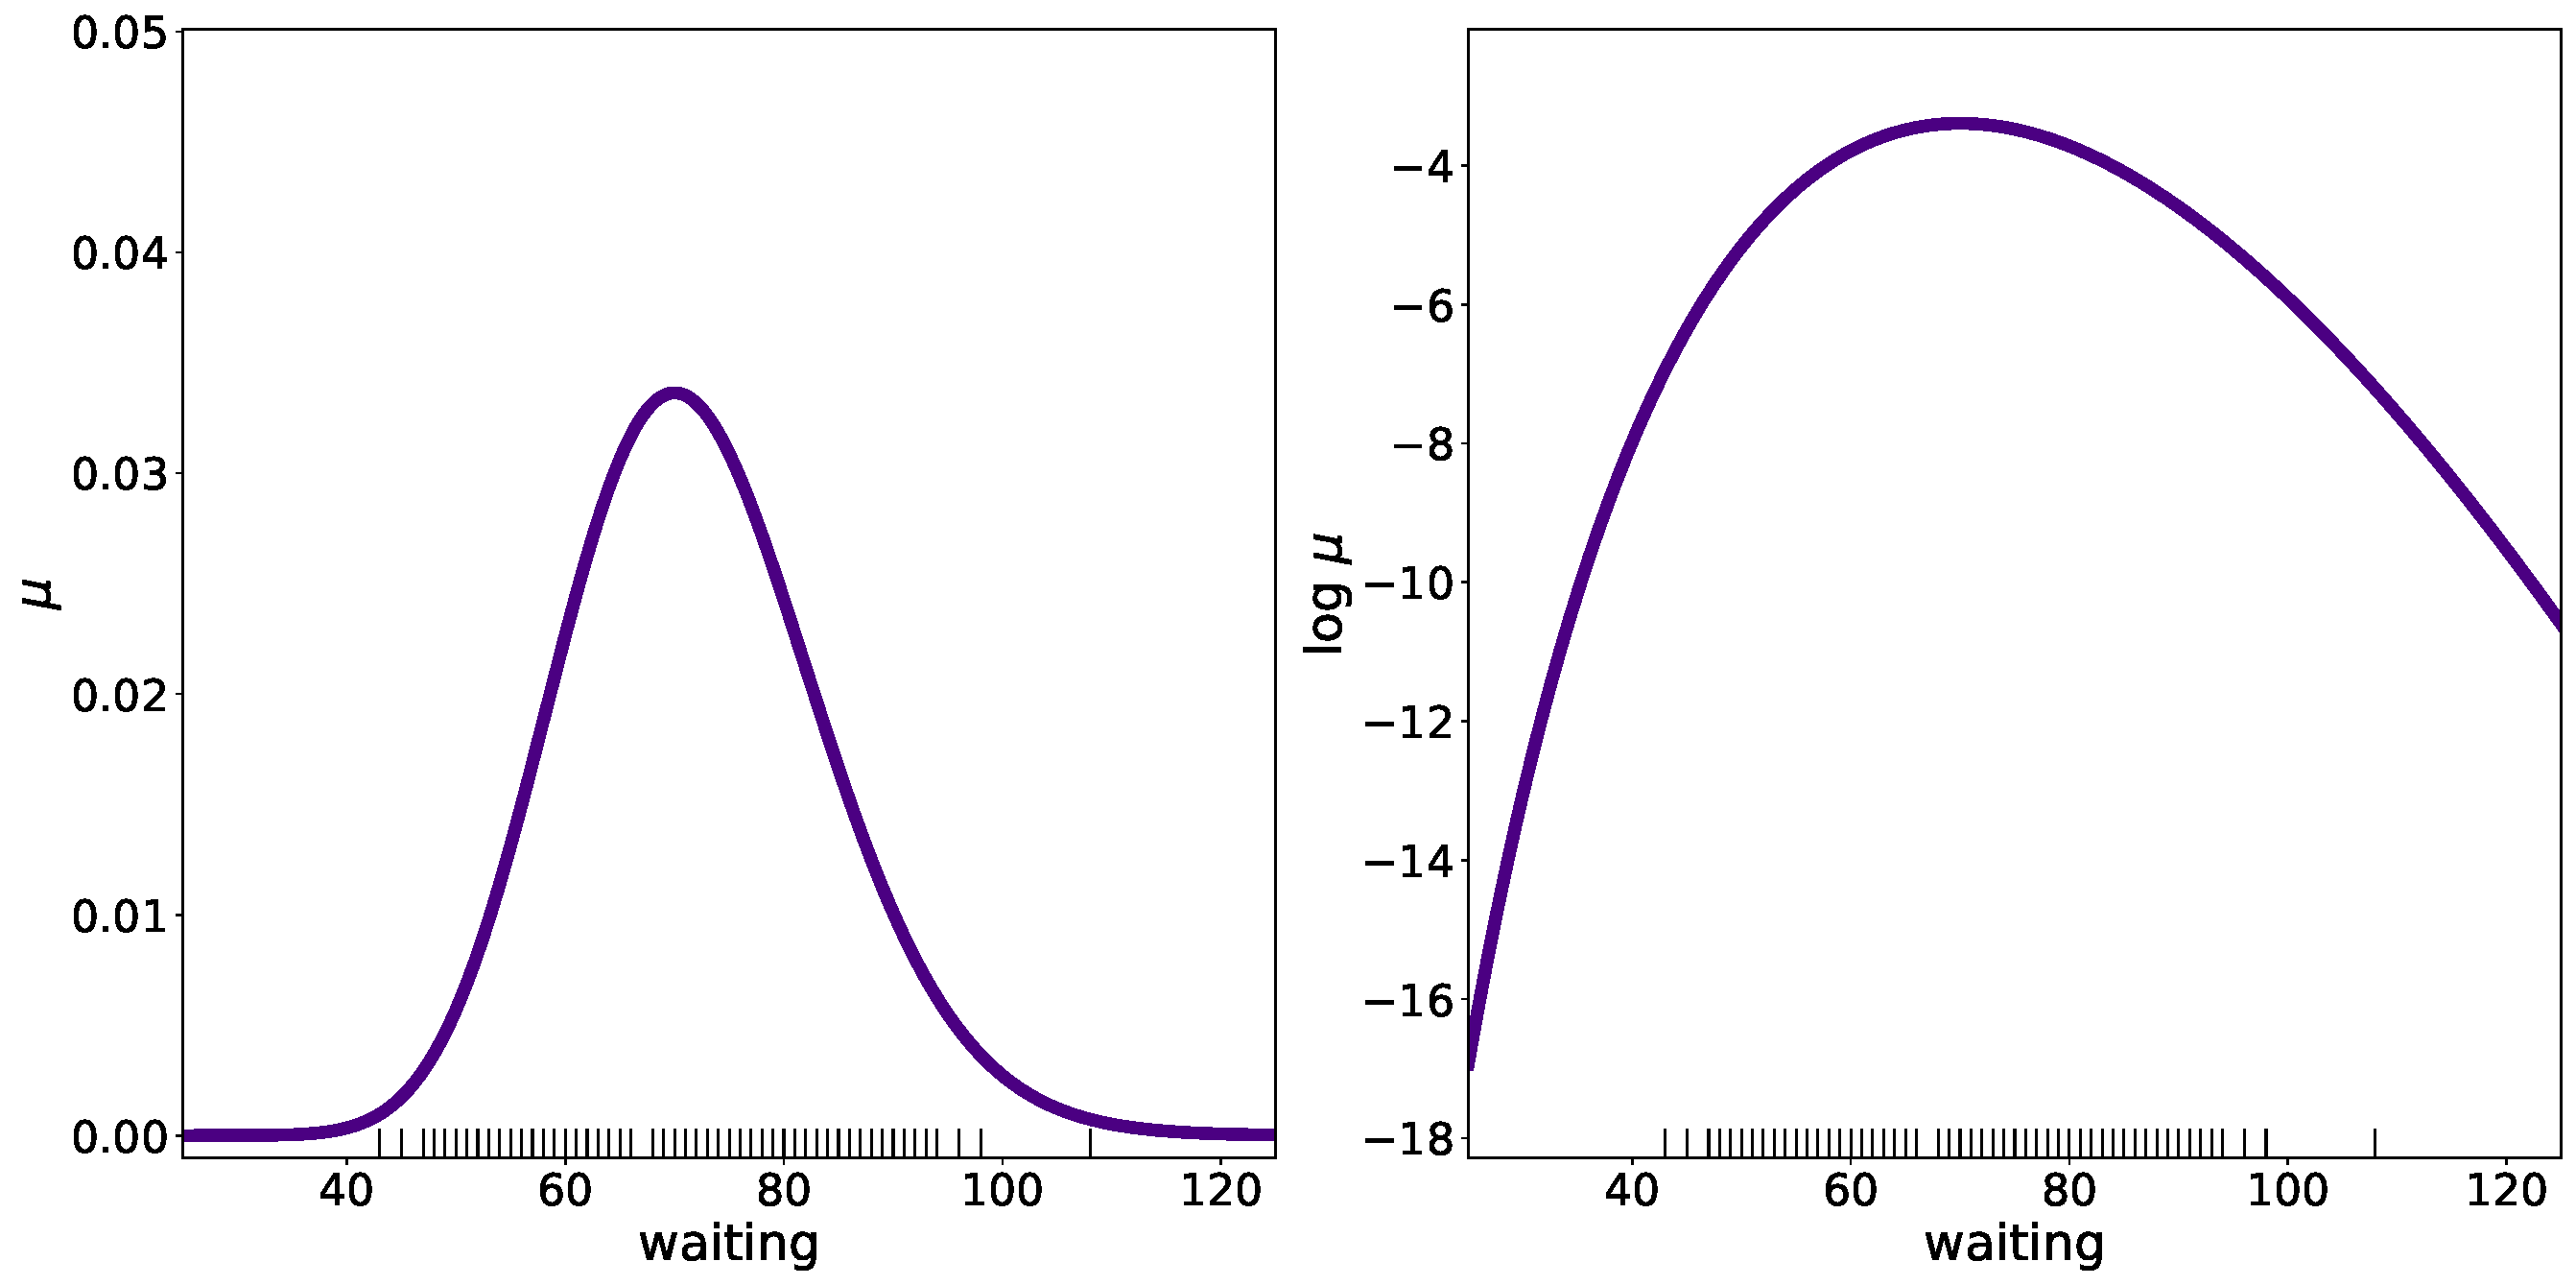
\includegraphics[width=\textwidth]{../plots/baseden-logbaseden-Gamma-36.0-2.0.pdf}
	\caption{Left panel shows $\mu$ and right panel shows $\log \mu$. The rug plot indicates the location of data.}
	\label{fig-base-den-log}
\end{figure}

The resulting early stopping SM density estimates are shown in Figure \ref{fig-early-stopping-estimate}. Note that when the number of iterations $t$ is small, the resulting density estimates are very close to $\mu$, as we expect. As $t$ increases, the density estimates become reasonable and show the bimodal feature of the data. However, as $t$ becomes very large, the density estimates contain a bump or become a spike at the isolated observation 108. We will return to this phenomenon in Section \ref{subsec-smes-limiting-t} and in the subsequent chapters of this dissertation. 

\begin{figure}[t]
	\centering
	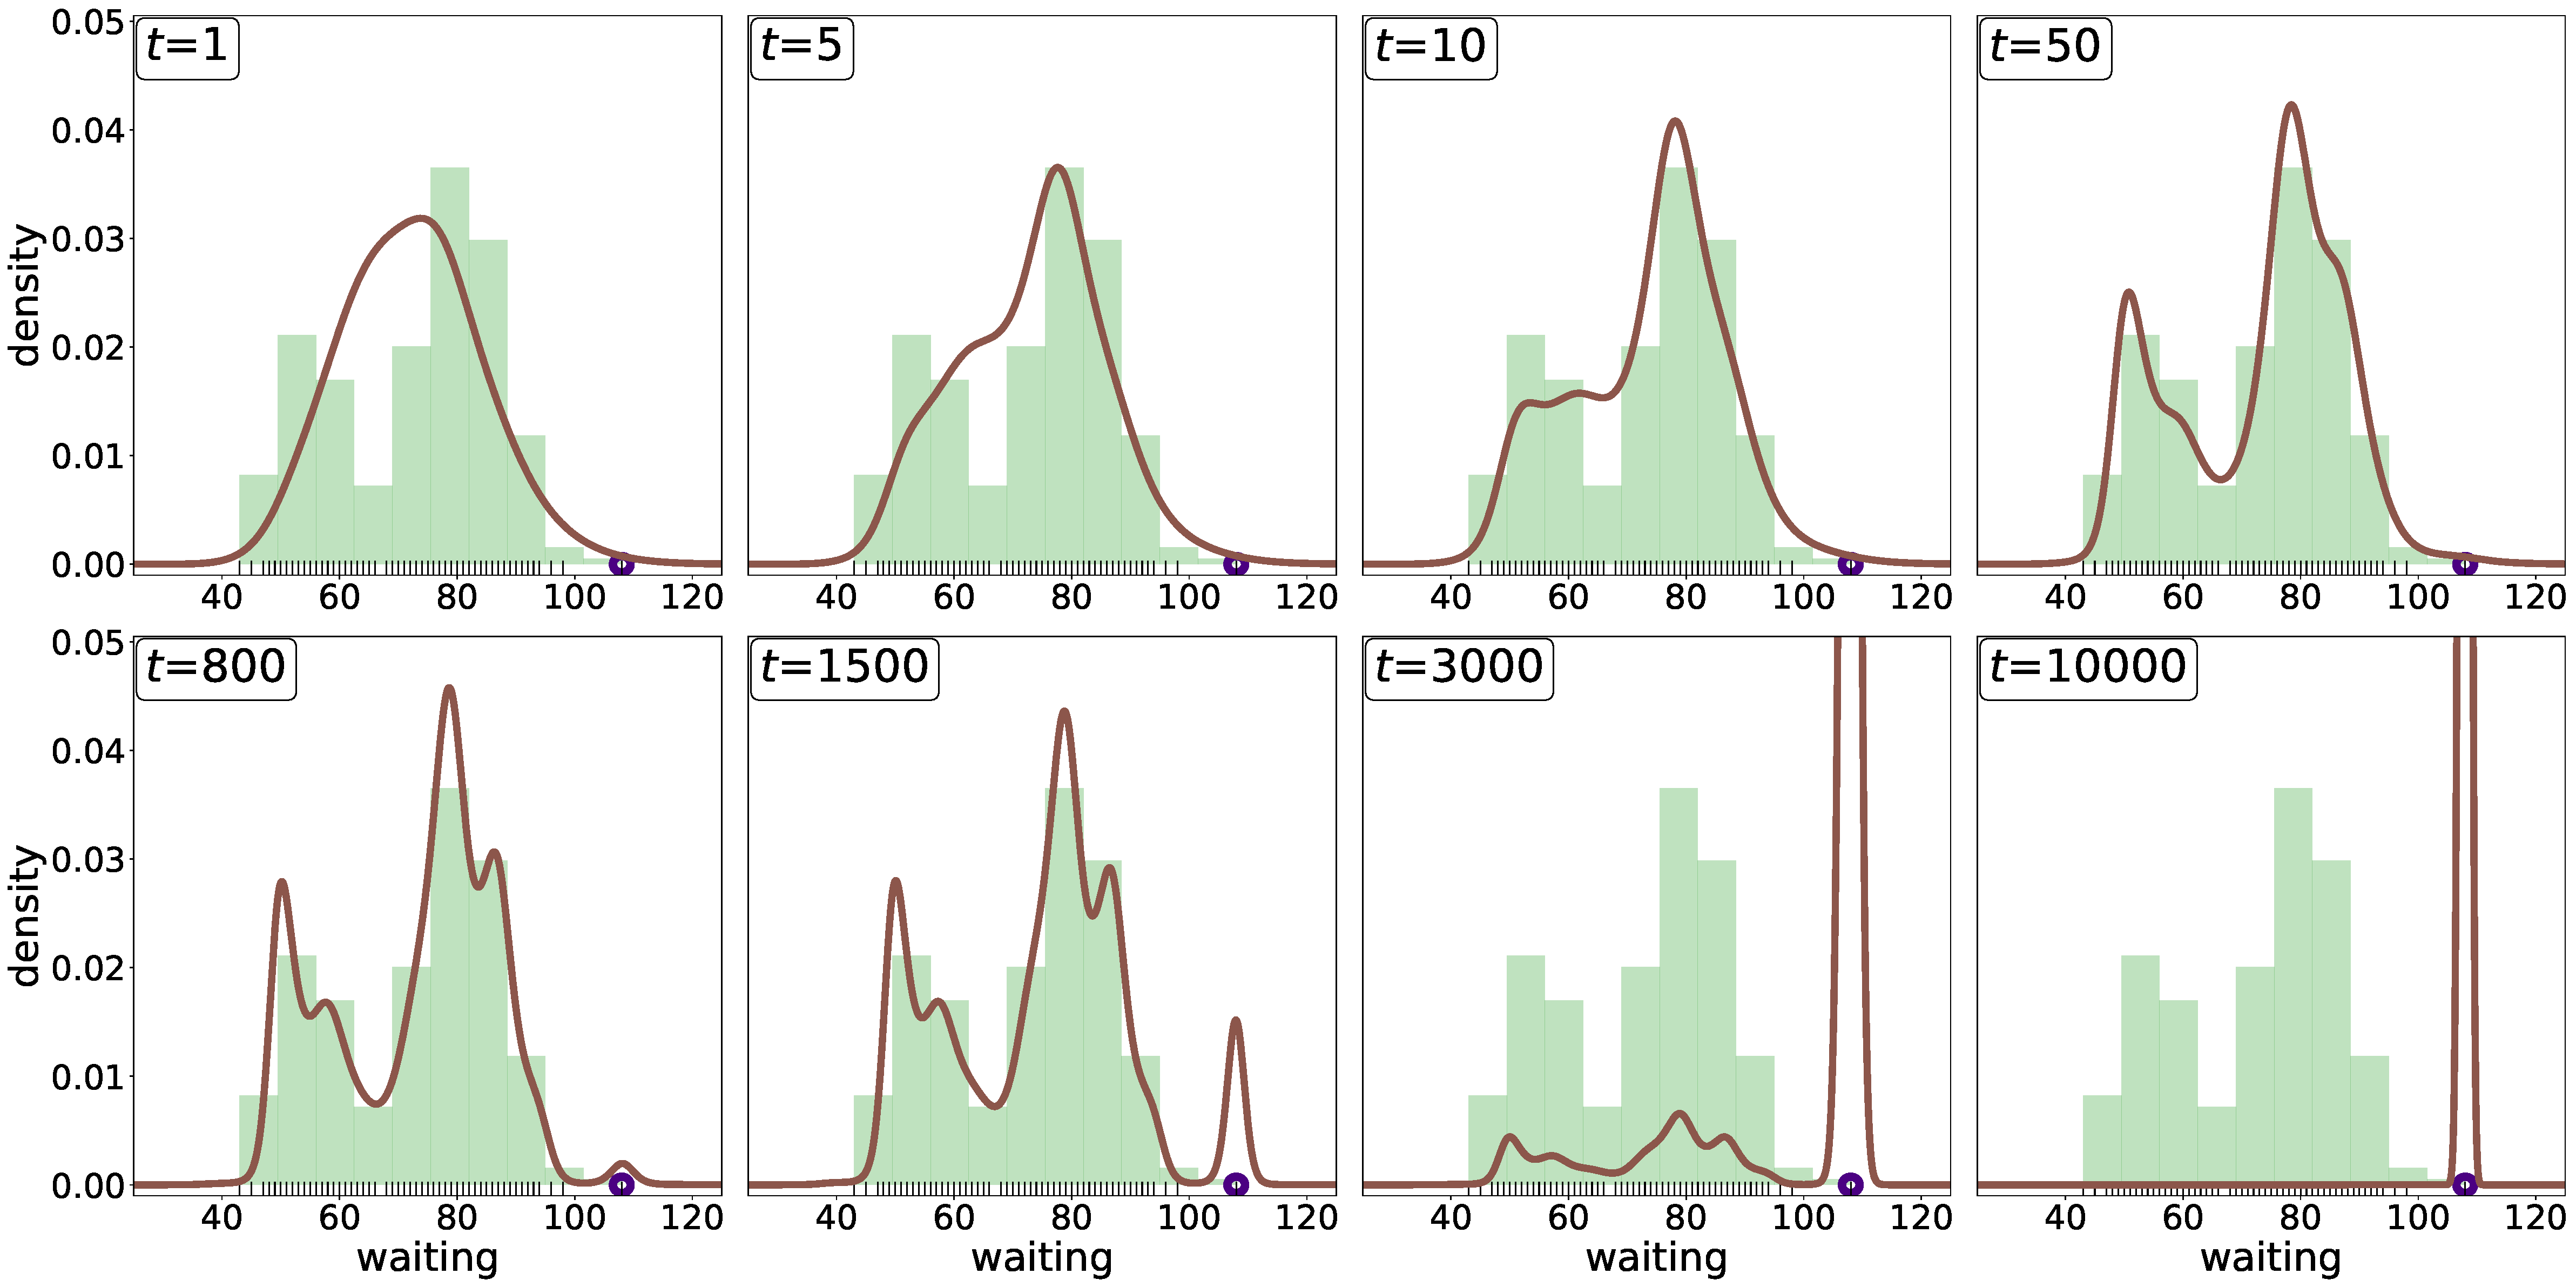
\includegraphics[width=\textwidth]{../plots/waiting-SM-density-estimates-earlystopping-only-bw=5.0-baseden=Gamma-36.0-2.0-entireRKHS.pdf}
	\caption{Early stopping SM density estimates for different values of number of iterations labeled at the upper left corner. Histogram of data with the bin width chosen by the Freedman-Diaconis rule is shown in green. The rug plot indicates the location of data and the purple circle indicates the location of the observation 108.}
	\label{fig-early-stopping-estimate}
\end{figure}

\subsection{When to Terminate the Algorithm}

With the numerical examples shown in the preceding section, we see the choice of the number of iterations is critical to producing satisfactory density estimates. The goal of this section is to discuss how to determine when to terminate the gradient descent algorithm in practice. We will provide two methods: the hold-out method and the $K$-fold cross validation. 

% We re-emphasize that the number of iterations $t$ in the early stopping approach performs the regularization purpose. If we stop too early, 

The hold-out method randomly partition the entire data into two parts, where one part, denoted by $\bS_{\mathrm{train}}$, 
%:= \sets{X_{\sigma \parens{1}}, \cdots, X_{\sigma \parens{m}}}$, 
is used to perform the gradient descent algorithm and the other part, denoted by $\bS_{\mathrm{test}}$, 
%:= \sets{X_{\sigma \parens{m+1}}, \cdots, X_{\sigma \parens{n}}}$
is used to evaluate the performance of the corresponding gradient descent iterate. 
%, where $\sigma \parens{i}$ denotes the index of data after the random shuffling for all $i = 1, \cdots, n$. 
%Let 
%\begin{align*}
%	\widehat{J}_{\SM, \mathrm{train}} \parens{f} := \frac{1}{2} \innerp{f}{\widehat{C}_{\mathrm{train}} f}_{\calH} - \innerp{f}{\hat{z}_{\mathrm{train}}}_{\calH}, \qquad \widehat{J}_{\SM, \mathrm{test}} \parens{f} := \frac{1}{2} \innerp{f}{\widehat{C}_{\mathrm{test}} f}_{\calH} - \innerp{f}{\hat{z}_{\mathrm{test}}}_{\calH}
%\end{align*}
%where 
%\begin{align*}
%	\widehat{C}_{\mathrm{train}} := \frac{1}{m} \sum_{i=1}^m \sum_{u=1}^d \partial_u k \parens{X_{\sigma \parens{i}}, \,\cdot\,} \otimes \partial_u k \parens{X_{\sigma \parens{i}}, \,\cdot\,}
%\end{align*}
Let $\widehat{J}_{\SM, \mathrm{train}}$ and $\widehat{J}_{\SM, \mathrm{test}}$ be the SM loss functionals constructed using data in $\bS_{\mathrm{train}}$ and data in $\bS_{\mathrm{test}}$, respectively. Starting from $\hat{f}^{\parens{0}} = 0$, we perform the gradient descent algorithm on $\widehat{J}_{\SM, \mathrm{train}}$, and after obtaining a gradient descent iterate $\hat{f}^{\parens{t}}$, we compute $\widehat{J}_{\SM, \mathrm{test}} \parens{\hat{f}^{\parens{t}}}$, and terminate when $\widehat{J}_{\SM, \mathrm{test}} \parens{\hat{f}^{\parens{t+1}}} > \widehat{J}_{\SM, \mathrm{test}} \parens{\hat{f}^{\parens{t}}}$. The algorithm is shown in Algorithm \ref{algo-early-stopping-holdout}. 

\begin{algorithm}
\caption{Hold-out method to determine when to terminate}\label{algo-early-stopping-holdout}
\begin{algorithmic}[1]
\Statex \algorithmicrequire 
\begin{itemize}\setlength\itemsep{0em}
	\item $X_1, \cdots, X_n$, the data from $p_0$; 
	\item $m < n$, the number of observations in $\bS_{\mathrm{train}}$; 
	\item $\tau$, the constant step size. 
\end{itemize}

\State Randomly shuffle the data $X_1, \cdots, X_n$, and let the first $m$ observations be $\bS_{\mathrm{train}}$ and the remaining be $\bS_{\mathrm{test}}$; 
\State Let \texttt{error1} = $\widehat{J}_{\SM, \mathrm{test}} \parens{\hat{f}^{\mathtt{old}}}$, where $\hat{f}^{\mathtt{old}} = \hat{f}^{\parens{0}} = 0$; 
\State Let $\hat{f}^{\mathtt{new}} = \hat{f}^{\mathtt{old}} - \tau \nabla \widehat{J}_{\SM, \mathrm{train}} \parens{\hat{f}^{\mathtt{old}}}$; 
\State Compute \texttt{error2} = $\widehat{J}_{\SM, \mathrm{test}} \parens{\hat{f}^{\mathtt{new}}}$; 
\While{\texttt{error1} $>$ \texttt{error2}}
\State Let $\hat{f}^{\mathtt{old}} = \hat{f}^{\mathtt{new}}$ and \texttt{error1} = \texttt{error2};  
\State Update $\hat{f}^{\mathtt{new}} = \hat{f}^{\mathtt{old}} - \tau \nabla \widehat{J}_{\SM, \mathrm{train}} \parens{\hat{f}^{\mathtt{old}}}$; 
\State Compute \texttt{error2} = $\widehat{J}_{\SM, \mathrm{test}} \parens{\hat{f}^{\mathtt{new}}}$; 
\EndWhile
\State \Return $\hat{f}^{\mathtt{old}}$. 
\end{algorithmic}
\end{algorithm}

The major drawback of this hold-out method is that it has to set aside a portion of data for the evaluation purpose, rather than use the entire data for the estimation purpose. 

The second method is the $K$-fold cross-validation (CV). We first specify a set of number of iterations candidates to terminate the algorithm, and randomly partition all data into $K$ folds of (roughly) equal size. Let us fix one number of iterations candidate, say $t_0$, for now. We use $K-1$ folds of data to perform the gradient descent algorithm and terminate at $t_0$, and evaluate the SM loss functional constructed using data in the remaining fold at this gradient descent iterate. Note that, for this particular $t_0$, we end up with $K$ values of the SM loss functional, one obtained from each fold. We average all these $K$ values and regard this average as the estimated risk of $t_0$. Repeat this process for each number of iterations candidate, and obtain an estimated risk from each of them. The best number of iterations is the one with the lowest estimated risk. In the end, we perform the gradient descent algorithm on the entire data and terminate at this best number of iterations. It is obvious that the final early stopping SM density estimate utilizes all data and avoid the drawback in the hold-out method. The complete algorithm of this $K$-fold CV method is shown in Algorithm \ref{algo-early-stopping-cv}. 

\begin{algorithm}
\caption{$K$-fold cross-validation method to determine when to terminate}\label{algo-early-stopping-cv}
\begin{algorithmic}[1]
\Statex \algorithmicrequire 
\begin{itemize}\setlength\itemsep{0em}
	\item $X_1, \cdots, X_n$, the data from $p_0$; 
	\item $K$, the number of folds for cross validation; 
	\item $\tau$, the constant step size; 
	\item $t_1, \cdots, t_m$, a list of number of iterations candidates to terminate. 
\end{itemize}

\State Randomly partition the data $X_1, \cdots, X_n$ into $K$ folds of (roughly) equal size, denoted by $\bS_{1}, \cdots, \bS_{K}$; 
\State Set \texttt{metric} to be an empty list to record the estimated risks for different number of iterations candidates; 
\For{$j = 1, \cdots, m$}
\State Set \texttt{metric\_j} = 0; 
\For{$\ell = 1, \cdots, K$}
\State Let $\bS_{\mathrm{test}} = \bS_{\ell}$ and $\bS_{\mathrm{train}}$ contain data excluding $\bS_{\ell}$; 
\State Perform the gradient descent algorithm on $\widehat{J}_{\SM, \mathrm{train}}$, which is the SM loss functional constructed using data in $\bS_{\mathrm{train}}$, and terminate at $t_j$; denote the resulting natural parameter by $\hat{f}_{\ell}^{\parens{t_j}}$; 
\State Update \texttt{metric\_j} += $\widehat{J}_{\SM, \mathrm{test}} \parens{\hat{f}_{\ell}^{\parens{t_j}}}$, where $\widehat{J}_{\SM, \mathrm{test}}$ is the SM loss functional constructed using data in $\bS_{\mathrm{test}}$; 
\EndFor
\State Append \texttt{metric\_j}/$K$ to the end of \texttt{metric}; 
\EndFor
\State Let $m^* \in \sets{1, \cdots, m}$ be the one with the lowest value in \texttt{metric}. Then, $t_{m^*}$ is the best number of iterations; 
\State Perform the gradient descent algorithm on $\widehat{J}_{\SM}$, the SM loss functional constructed using \emph{all} data, and terminate at $t_{m^*}$. 
\State \Return $\hat{f}^{\parens{t_{m^*}}}$. 
\end{algorithmic}
\end{algorithm}


\section{Theoretical Properties}\label{section-theoretical-properties}

With the introduction to our early stopping SM density estimator and its computation, we discuss its theoretical properties in this section. 

We will assess its theoretical properties from two aspects. First, we will look at what happens to the density estimator if we do not terminate the gradient descent algorithm and let the number of iterations approach to $\infty$. This will be covered in Section \ref{subsec-smes-limiting-t}. 

Second, in this early stopping approach, we use the number of iterations as a tuning parameter to perform implicit regularization, which plays exactly the same role as the penalty parameter $\rho$ in the penalized approach. We derive a (theoretical) stopping rule and establish the convergence rates of the resulting natural parameter estimator and the density estimator using this stopping rule in Section \ref{subsec-nonasymp-t}.

\subsection{Density Estimator Without Termination} \label{subsec-smes-limiting-t}

In this section, we investigate the behavior of the early stopping SM density estimator if we keep running the gradient descent algorithm without termination. 

Our main theorem is the following. 

\begin{theorem}\label{thm-limiting-density-t}
	Let $\hat{z}_2 \in \calH$ be the orthogonal projection of $\hat{z}$ onto $\range \parens{\widehat{C}}^{\perp}$, the orthogonal complement of $\range \parens{\widehat{C}}$. In addition to \ref{assumption-2-1-inf-dim} - \ref{assumption-2-4-base-density} in Chapter \ref{ch2} and \ref{assumption-1} - \ref{assumption-5}, we further assume 
	\begin{enumerate}[label=\textbf{(C\arabic*)}]
		\item \label{assumption-limiting-1} there exists a unique $x^* \in \calX$ such that 
		%$\hat{z}_2 \parens{x^*} \ge \hat{z}_1 \parens{x}$ for all $x \in \calX$ and 
		$\hat{z}_2 \parens{x^*} > \hat{z}_2 \parens{x}$ for all $x \in \calX \backslash \sets{x^*}$, and 
		\item \label{assumption-limiting-2} $\tau \in \parens{0, 1 / \parens{d \kappa_2^2}}$. 
	\end{enumerate}
	Then, $\lim_{t \to \infty} q_{\hat{f}^{\parens{t}}} \parens{x^*} = \infty$. 
\end{theorem}

\begin{remark}
	We can relax \ref{assumption-limiting-1} to the one that the maximizers of $\hat{z}_2$ form a set of Lebesgue measure zero. Let $\calM$ denote the set of all maximizers of $\hat{z}_2$. Then, we can modify the proof slightly and conclude $\lim_{t \to \infty} q_{\hat{f}^{\parens{t}}} \parens{x^*} = \infty$ at all $x^* \in \calM$. 
\end{remark}

The proof of Theorem \ref{thm-limiting-density-t} will be provided in Section \ref{subsection-proof-smes-limiting-t}, and is built upon the decomposition of $\hat{f}^{\parens{t}}$ which we now look at. 

\subsubsection{Decomposition of Gradient Descent Iterates}

We decompose $\hat{f}^{\parens{t}}$ into two parts, where one part resides in $\range \parens{\widehat{C}}$ and the other resides in $\range \parens{\widehat{C}}^{\perp}$, the orthogonal complement of $\range \parens{\widehat{C}}$. 

As we have discussed in Section \ref{subsection-first-algorithm}, $\range \parens{\widehat{C}}$ contains all functions that can be written as a linear combination of $\partial_u k \parens{X_i, \,\cdot\,}$, for all $i = 1, \cdots, n$ and $u = 1, \cdots, d$, which is of finite dimension and forms a closed linear subspace of $\calH$ \parencite[Corollary 6 in Section 13.3 in][]{Royden2018-cd}. Its orthogonal complement is 
\begin{align*}
	\range \parens{\widehat{C}}^{\perp} := \sets[\Big]{g \in \calH \Bigm| \innerp{g}{f}_{\calH} = 0, \text{ for all } f \in \range \parens{\widehat{C}}}, 
\end{align*}
which also forms a closed linear subspace of $\calH$ \parencite[Section 16.1 in][]{Royden2018-cd}.  

Notice that $\range \parens{\widehat{C}}^{\perp} \neq \sets{0}$. To see this, suppose the opposite. Then, we have $\range \parens{\widehat{C}} = \calH$ \parencite[Corollary 4 in Section 16.1 in][]{Royden2018-cd}. But, since $\range \parens{\widehat{C}}$ is finite-dimensional, $\range \parens{\widehat{C}} = \calH$ implies $\calH$ is also finite-dimensional. This contradicts to \ref{assumption-2-1-inf-dim} in Chapter \ref{ch2} that $\calH$ is infinite-dimensional. 

Now, decompose $\hat{z}$ into two parts, $\hat{z}_1$ and $\hat{z}_2$, where $\hat{z}_1 := \Pi_{\range \parens{\widehat{C}}} \parens{\hat{z}} \in \range \parens{\widehat{C}}$, $\hat{z}_2 := \Pi_{\range \parens{\widehat{C}}^{\perp}} \parens{\hat{z}} \in \range \parens{\widehat{C}}^{\perp}$, and $\Pi_S \parens{\hat{z}}$ denotes the orthogonal projection of $\hat{z}$ onto the closed linear subspace $S$ of $\calH$. Note that both $\hat{z}_1$ and $\hat{z}_2$ are well-defined by the projection theorem in a Hilbert space \parencite[Theorem 2.3.1 in][]{Brockwell2013-dq}. 

Recall that $\hat{z} = - \frac{1}{n} \sum_{i=1}^n \sum_{u=1}^d \parens[\big]{\parens{\partial_u \log \mu} \parens{X_i} \partial_u k \parens{X_i, \,\cdot\,} + \partial_u^2 k \parens{X_i, \,\cdot\,}}$ involves the first two partial derivatives of $k$. The component $- \frac{1}{n} \sum_{i=1}^n \sum_{u=1}^d \partial_u \log \mu \parens{X_i} \partial_u k \parens{X_i, \,\cdot\,}$ must belong to $\range \parens{\widehat{C}}$, and the component $- \frac{1}{n} \sum_{i=1}^n \sum_{u=1}^d \partial_u^2 k \parens{X_i, \,\cdot\,}$ does \emph{not} necessarily belong to $\range \parens{\widehat{C}}$, except for special choices of $k$. We assume $\hat{z}_2 \neq 0$ for the rest of this section. 

In addition, since $\hat{z}_1 \in \range \parens{\widehat{C}}$, we can find $\hat{g}_1 \in \range \parens{\widehat{C}}$ satisfying $\hat{z}_1 = \widehat{C} \hat{g}_1$. We claim such a choice of $\hat{g}_1$ is unique. Suppose there exists $\tilde{g}_1 \in \range \parens{\widehat{C}}$ and $\tilde{g}_1 \neq \hat{g}_1$ such that $\hat{z}_1 = \widehat{C} \tilde{g}_1$, then $0 = \widehat{C} \parens{\hat{g}_1 - \tilde{g}_1}$, implying that $\hat{g}_1 - \tilde{g}_1 = 0$ or $\hat{g}_1 - \tilde{g}_1 \in \range \parens{\widehat{C}}^{\perp}$ is nonzero. Since $\range \parens{\widehat{C}}$ is a closed linear subspace of $\calH$, the latter case cannot happen. We deduce that $\tilde{g}_1 = \hat{g}_1$, and the uniqueness follows. 

With the decomposition of $\hat{z}$ we have discussed so far, the following proposition decomposes $\hat{f}^{\parens{t}}$ into two components. %, where one component belongs to $\range \parens{\widehat{C}}$ and the other belongs to $\range \parens{\widehat{C}}^{\perp}$. 

\begin{proposition}\label{prop-decomposition-ft}
	Suppose $\hat{f}^{\parens{0}} = 0 \in \calH$. The $\parens{t+1}$-st gradient descent iterate $\hat{f}^{\parens{t+1}}$, for each $t \in \Natural_0$, can be written as the sum of the following two components 
	\begin{align*}
		\hat{f}_1^{\parens{t+1}} := & \,  \parens{I - \parens{I - \tau \widehat{C}}^{t+1}} \hat{g}_1 \in \range \parens{\widehat{C}}\\ 
		\hat{f}_2^{\parens{t+1}} := & \, \parens{t+1} \tau \hat{z}_2 \in \range \parens{\widehat{C}}^{\perp}
	\end{align*}
\end{proposition}

The following proposition gives explicit formulae for $\hat{z}_1$, $\hat{z}_2$, and $\hat{g}_1$. 

\begin{proposition}\label{prop-hatz1-hatz2-g1}
	Let $\bG \in \Real^{nd \times nd}$ and $\bh \in \Real^{nd}$ be the quantities defined in Theorem \ref{thm-early-stopping-algo} and assume $\bG$ is positive definite. Then, 
	\begin{enumerate}[label=(\alph*)]
		\item \label{prop-hatz1-hatz2-g1-1} $\hat{z}_1 = \sum_{i=1}^n \sum_{u=1}^d \alpha^*_{\parens{i-1}d+u} \partial_u k \parens{X_i, \,\cdot\,}$, where $\balpha^* := \parens{\alpha^*_{1}, \cdots, \alpha^*_{nd}} \in \Real^{nd}$ satisfies the linear system $\bG \balpha^* = \bh$; 
		\item \label{prop-hatz1-hatz2-g1-2} $\hat{z}_2 = \sum_{i=1}^n \sum_{u=1}^d \bracks[\big]{ \parens[\big]{- \frac{1}{n} \parens{\partial_u \log \mu} \parens{X_i} - \alpha^*_{\parens{i-1}d+u}} \partial_u k \parens{X_i, \,\cdot\,} - \frac{1}{n} \partial_u^2 k \parens{X_i, \,\cdot\,}}$; 
		\item \label{prop-hatz1-hatz2-g1-3} $\hat{g}_1 = \sum_{i=1}^n \sum_{u=1}^d \beta^*_{\parens{i-1}d+u} \partial_u k \parens{X_i, \,\cdot\,}$, where $\bbeta^* := \parens{\beta_1^*, \cdots, \beta_{nd}^*} \in \Real^{nd}$ satisfies the linear system $\frac{1}{n} \bG \bbeta^* = \balpha^*$. 
	\end{enumerate}
\end{proposition}

Now that we have decomposed $\hat{f}^{\parens{t+1}}$ into two components, the following proposition established the boundedness of $\hat{f}_1^{\parens{t+1}}$ over $\calX$ for all $t \in \Natural_0$. 

\begin{proposition}\label{proposition-bound-hatz1}
	Under the same assumptions in Theorem \ref{thm-limiting-density-t}, there exists $M > 0$ such that, for all $x \in \calX$ and all $t \in \Natural_0$, $\abs{\innerp{\hat{f}_1^{\parens{t+1}}}{k \parens{x, \,\cdot\,}}_{\calH}} \le M$. 
\end{proposition}

The proofs of Propositions \ref{prop-decomposition-ft} - \ref{proposition-bound-hatz1} can be found in Section \ref{subsection-proof-smes-limiting-t}. 

Even though $\hat{f}_1^{\parens{t+1}}$ is bounded over $\calX$ for all $t \in \Natural_0$, $\hat{f}_2^{\parens{t+1}}$ is \emph{not}. In particular, since $\hat{f}_2^{\parens{t+1}} = \parens{t+1} \tau \hat{z}_2$, we have 
\begin{align*}
	\abs{ \innerp{\hat{f}_2^{\parens{t+1}}}{ k \parens{x, \,\cdot\,}}_{\calH} } = \parens{t+1} \tau \abs{\innerp{\hat{z}_2}{k \parens{x, \,\cdot\,}}_{\calH} } \to \infty, \qquad \text{ as } t \to \infty, 
\end{align*}
unless $\innerp{\hat{z}_2}{k \parens{x, \,\cdot\,}}_{\calH} = 0$. 


\subsubsection{Numerical Illustration of Theorem \ref{thm-limiting-density-t}}

We use the \texttt{waiting} variable in the Old Faithful Geyser dataset to illustrate Theorem \ref{thm-limiting-density-t}. 

With the help of \eqref{eq-hatz} in Chapter \ref{ch2} and Proposition \ref{prop-hatz1-hatz2-g1}, we plot $\hat{z}$, $\hat{z}_1$ and $\hat{z}_2$ in Figure \ref{fig-decomposition-hatz}. In particular, note that, from the right panel of Figure \ref{fig-decomposition-hatz}, $\hat{z}_2$ achieves the maximum at $108$. With Theorem \ref{thm-limiting-density-t}, we expect see that, as the number of iterations $t$ keeps increasing, the density value at $108$ also keeps increasing. Figure \ref{fig-density-val-108-vs-t}, the plot of the density value at 108 against the number of iterations, coincides with our expectation. 

\begin{figure}[t]
	\centering
	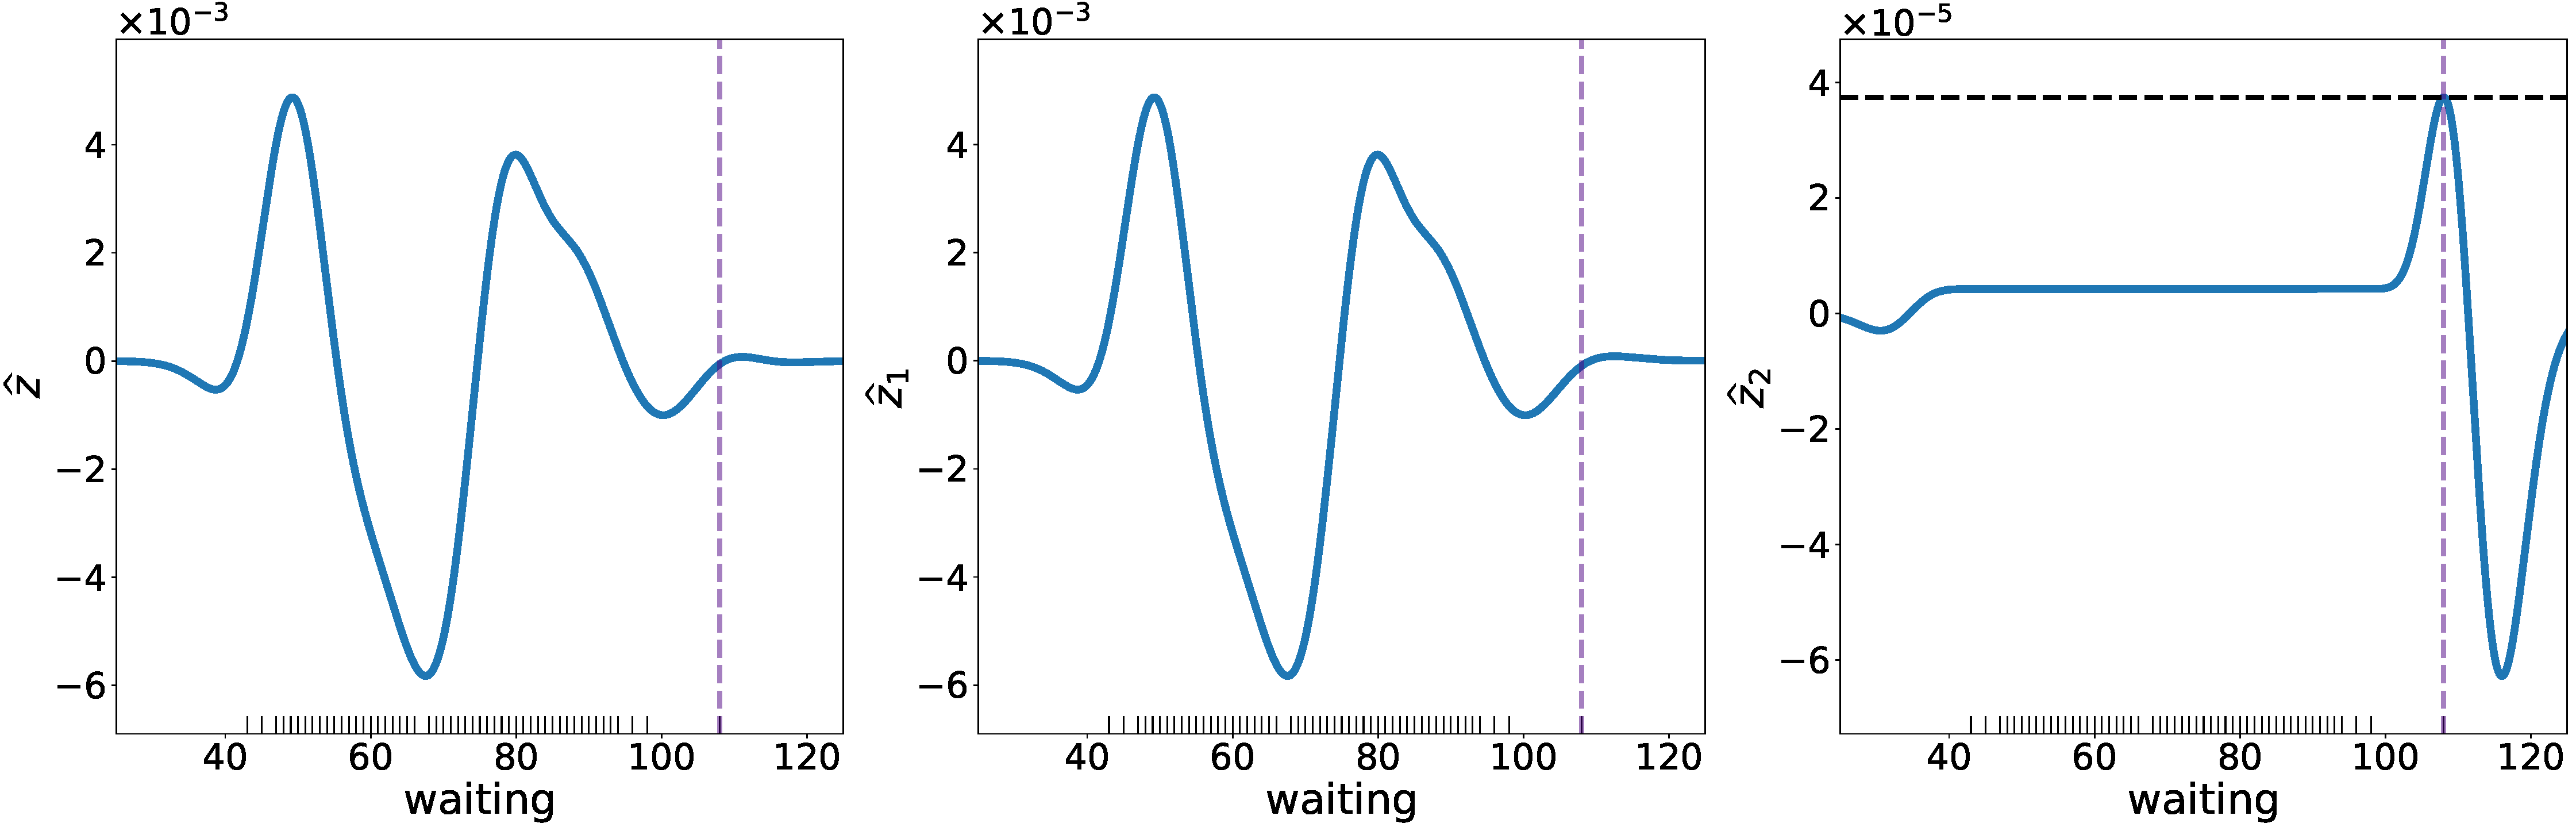
\includegraphics[width=\textwidth]{../plots/decomposition-hat-z-bw=5.0-Gamma-36.0-2.0.pdf}
	\caption{Plots of $\hat{z}$ (left panel), $\hat{z}_1$ (middle panel) and $\hat{z}_2$ (right panel). The rug plot indicates the location of data.}
	\label{fig-decomposition-hatz}
\end{figure}

\begin{figure}[h]
	\centering
	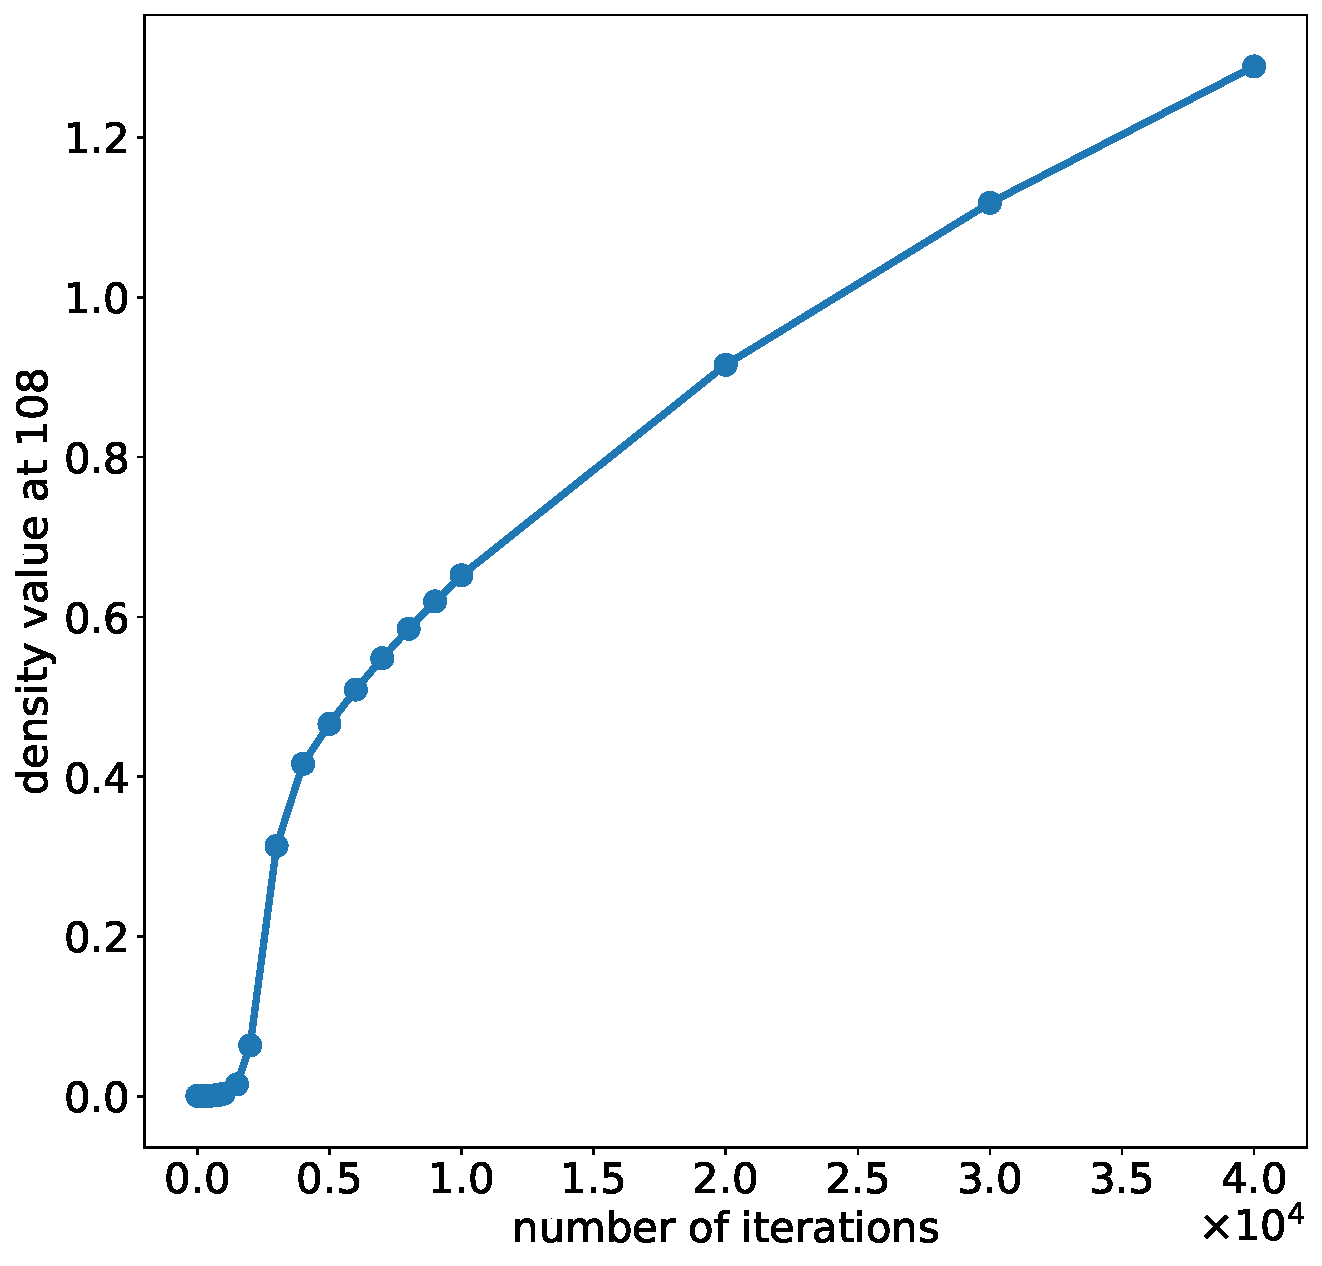
\includegraphics[width=0.6\textwidth]{../plots/density-at-108-vs-number-iterations-Gamma-36.0-2.0.pdf}
	\caption{Density value at $108$ against the number of iterations.}
	\label{fig-density-val-108-vs-t}
\end{figure}

\subsection{Rate of Convergence} \label{subsec-nonasymp-t}

We study the rate of convergence of the early stopping SM density estimator in this section. More specifically, we attempt to answer the following questions: 
\begin{enumerate}
	% \item What is the (theoretically) optimal number of iterations? In what sense is this number of iterations optimal? 
	\item Suppose $p_0 = q_{f_0} \in \calQ_{\ker}$ for some $f_0 \in \calH$. What can we say about the gap between $\hat{f}^{\parens{t}}$ and $f_0$, for each $t \in \Natural$? 
	\item What can we say about the gap between $q_{\hat{f}^{\parens{t}}}$ and $p_0$, for each $t \in \Natural$? 
	\item Based on the gaps above, can we derive an early stopping rule? 
\end{enumerate}

Throughout this section, besides \ref{assumption-1} - \ref{assumption-5}, we further assume the following: 
\begin{enumerate}[label=\textbf{(B\arabic*)}, resume=assumptions]
	\item \label{assumption-6} The true density $p_0$ belongs to $\calQ_{\ker}$ and there exists $f_0 \in \calH$ such that $p_0 = q_{f_0}$. % https://tex.stackexchange.com/questions/455028/continuing-the-enumerate-numbering-from-other-the-enumerate-list-in-the-document, continue the numbering from the previous enumeration 
	\item \label{assumption-7} There exists $\gamma > 0$ such that $f_0 \in \range \parens{C^\gamma}$, where $C: \calH \to \calH$ is given by \eqref{eq-C-def}. That is, there exists $g_0 \in \calH$ such that $C^{\gamma} g_0 = f_0$. 
\end{enumerate}

Our main result is the following theorem. 

\begin{theorem}\label{theorem-convergence-rate}
	Under \ref{assumption-2-1-inf-dim} - \ref{assumption-2-4-base-density} in Chapter \ref{ch2} and \ref{assumption-1} - \ref{assumption-7}, for each $n \in \Natural$, there exists an early stopping rule 
	\begin{align*}
		t^*: \Natural & \, \to \Natural, \qquad \qquad n \mapsto \ceil{n^{\frac{1}{2 \parens{\gamma + 2}}}}
	\end{align*}
	such that, with probability at least $1 - \delta$ for $\delta \in \parens{0, 1}$, the following inequality holds 
	\begin{align*}
		\norm{\hat{f}^{\parens{t^* \parens{n}}} - f_0}_{\calH} \le & \, \parens{4 C_1 + C_2} n^{-\frac{\gamma}{2 \parens{\gamma+2}}}, 
	\end{align*}
	where $C_1 := 2d\tau \parens{\kappa_3 + \kappa_4} \parens{\tau d \kappa_2^2 + 1} \sqrt{2 \log \parens{2 / \delta}}$ and $C_2 := \gamma^{\gamma} \norm{g_0}_{\calH} / \parens{\tau e}^{\gamma}$. 
\end{theorem}

The proof follows \textcite{Yao2007-ji} and details will be provided in Section \ref{proof-theorem-convergence-rate}. The proof depends on the analysis of two sequences of gradient descent iterates: one is the gradient descent iterates derived from the SM loss functional $\widehat{J}_{\SM}$ (which depends on finitely many samples) and the other one is the gradient descent iterates derived from the H-divergence $J_{\SM} \parens{f}$ which can be viewed as the SM loss functional with infinitely many samples, i.e., the population-version SM loss functional. We denote the former sequence by $\sets{\hat{f}^{\parens{t}}}_{t \in \Natural}$ as before and the latter one by $\sets{f^{\parens{t}}}_{t \in \Natural}$, and let both start from the zero function, i.e., $f^{\parens{0}} = \hat{f}^{\parens{0}} = 0 \in \calH$. Using the triangle inequality, we can bound $\norm{\hat{f}^{\parens{t}} - f_0}_{\calH}$ from above by 
\begin{align}\label{eq-sample-plus-approx-errors}
	\norm{\hat{f}^{\parens{t}} - f_0}_{\calH} \le \norm{\hat{f}^{\parens{t}} - f^{\parens{t}}}_{\calH} + \norm{f^{\parens{t}} - f_0}_{\calH}, 
\end{align}
where the population-version sequence of iterates $\sets{f^{\parens{t}}}_{t \in \Natural}$ is used as an intermediary. 

In \eqref{eq-sample-plus-approx-errors}, $\norm{f^{\parens{t}} - f_0}_{\calH}$ is called the \textit{approximation error} (or \textit{bias}), and $\norm{\hat{f}^{\parens{t}} - f^{\parens{t}}}_{\calH}$, is called the \textit{sample error} (or \textit{variance}). We will see later that, as $t$ increases, the derived upper bound of the sample error increases and that of the approximation error decreases. More specifically, as the gradient descent algorithm evolves, the population-version sequence of iterates $\sets{f^{\parens{t}}}_{t \in \Natural}$ converge to $f_0$ eventually but the sample-version sequence of iterates $\sets{\hat{f}^{\parens{t}}}_{t \in \Natural}$ do \emph{not}. Therefore, we have a bias-variance tradeoff we discussed earlier: if we stop the algorithm at a too early time, the resulting $\hat{f}^{\parens{t}}$ has a small variance but a large bias; and, on the other hand, if we keep running it and terminate too late, the resulting $\hat{f}^{\parens{t}}$ has a small bias but a large variance. By minimizing the sum of these two upper bounds, we can identify an early stopping rule. 

In the next two sections, we will focus on the approximation error and the sample error, respectively, and derive their upper bounds that will help us prove Theorem \ref{theorem-convergence-rate}. 

\subsubsection{An Upper Bound on the Approximation Error}

In this section, we focus on the problem of minimizing $J_{\SM}$ over $\calH$, discuss the population-version sequence of iterates $\sets{f^{\parens{t}}}_{t \in \Natural}$, and derive an upper bound for the approximation error $\norm{f^{\parens{t}} - f_0}_{\calH}$. 

\begin{proposition}[Frech{\'e}t gradient of $J_{\SM}$]\label{prop-pop-frechet-grad}
	Under \ref{assumption-2-1-inf-dim} - \ref{assumption-2-4-base-density} in Chapter \ref{ch2} and \ref{assumption-1} - \ref{assumption-5}, the Frech{\'e}t gradient of $J_{\SM}$, denoted by $\nabla J_{\SM}$, is a map from $\calH$ to $\calH$ given by $\nabla J_{\SM} \parens{f} = C f - z$ for all $f \in \calH$. 
\end{proposition}

The proof of Proposition \ref{prop-pop-frechet-grad} is almost identical to that of Theorem \ref{thm-grad-widehatJ} and is omitted here. 

With Proposition \ref{prop-pop-frechet-grad}, the population-version of gradient descent iterates are 
\begin{align*}
	f^{\parens{t+1}} = & \, f^{\parens{t}} - \tau \nabla J_{\SM} \parens{f^{\parens{t}}} 
	% = & \, f_t - \alpha \cdot \parens{Cf_t - z} \\ 
	= \parens{I - \tau C} f^{\parens{t}} + \tau z, \qquad \text{ for all } t \in \Natural_0, 
\end{align*}
where $\tau \in \parens{0, 1 / \parens{d \kappa_2^2}}$ is the constant step size and $f^{\parens{0}} \in \hil$ is the starting point. Using the same argument as that of Theorem \ref{thm-closed-form}, we can link $f^{\parens{t+1}}$ to $f^{\parens{0}}$ as
\begin{align*}% \label{eq-pop-iteration-closed-form}
	f^{\parens{t+1}} = & \, \parens{I - \tau C}^{t+1} f^{\parens{0}} + \tau \sum_{j=0}^t \parens{I - \tau C}^{t - j} z. 
\end{align*}

With all ingredients above, we can now derive an upper bound of the approximation error $\norm{f^{\parens{t}} - f_0}_{\hil}$. 

\begin{theorem}[An upper bound on the approximation error]\label{theorem-approx-error}
	Choose $f^{\parens{0}} = 0$ and the constant step size $\tau \in \parens{0, 1 / \parens{d \kappa_2^2}}$. Under the same assumptions in Theorem \ref{theorem-convergence-rate}, we have, for all $t \in \Natural$, 
	\begin{align*}
		\norm{f^{\parens{t}} - f_0}_{\calH} \le \parens[\bigg]{\frac{\gamma}{\tau e t}}^{\gamma} \norm{g_0}_{\hil}. 
	\end{align*}
\end{theorem}

The proof of Theorem \ref{theorem-approx-error} will be provided in Section \ref{proof-theorem-approx-error}. 

In particular, note that $\norm{f^{\parens{t}} - f_0}_{\calH} \le \parens[\big]{\parens{\frac{\gamma}{\tau e }}^{\gamma} \norm{g_0}_{\hil}} t^{-\gamma}$. If we let $t \to \infty$, we obtain $\norm{f^{\parens{t}} - f_0}_{\calH} \to 0$ and deduce $f^{\parens{t}} \to f_0$. %Therefore, as the gradient descent algorithm evolves, the approximation error decreases to 0 and the population-version iterates converge to the true natural parameter $f_0$. 

\subsubsection{An Upper Bound on the Sample Error}

In this section, we turn to the sample error $\norm{\hat{f}^{\parens{t}} - f^{\parens{t}}}_{\calH}$ and derive an upper bound of it. The main result is the following. 

\begin{theorem}[An upper bound of the sample error]\label{theorem-sample-error}
	For both population- and sample-version iterations, choose $f^{\parens{0}} = \hat{f}^{\parens{0}} = 0$ and the common constant step size $\tau \in \parens{0, 1/\parens{d \kappa_2^2}}$. Under the same assumptions in Theorem \ref{theorem-convergence-rate}, with probability at least $1 - \delta$ for $\delta \in \parens{0, 1}$, the following inequality holds 
	\begin{align*}% \label{eq-sample-error-upper-bound}
		\norm{\hat{f}^{\parens{t}} - f^{\parens{t}}}_{\calH} \le & \, 2 d \tau t^2 \parens{\kappa_3 + \kappa_4} \parens{\tau d \kappa_2^2 + 1} \sqrt{\frac{2}{n} \log \parens[\bigg]{\frac{2}{\delta}}},  
	\end{align*}
	for all $t \in \Natural$. 
\end{theorem}

The proof of Theorem \ref{theorem-sample-error} will be provided in Section \ref{proof-theorem-sample-error}. Note, in particular, that the gap between $\hat{f}^{\parens{t}}$ and $f^{\parens{t}}$ expands with $t$. 

\subsubsection{Upper Bounds on the Distances between Densities}

Theorem \ref{theorem-convergence-rate} establishes the stopping rule $t^*$ and the convergence rate of $\hat{f}^{\parens{t^* \parens{n}}}$. We can carry it over to bounding various distances between $p_0$ and $q_{\hat{f}^{\parens{t^* \parens{n}}}}$. The main result is the following corollary. 

\begin{corollary}[Various distances between $p_0$ and $q_{\hat{f}^{\parens{t^* \parens{n}}}}$]\label{corollary-density-distances}
	Under the same assumptions as in Theorem \ref{theorem-convergence-rate}, with the stopping rule $t^*$ therein, the following inequalities hold with probability at least $1 - \delta$ for $\delta \in \parens{0, 1}$, 
	\begin{enumerate}[label=(\alph*)]
		\item \label{corollary-density-distances-a} in terms of the H-divergence, 
		\begin{align*}
			\Hdiv \parens{p_0 \Vert q_{\hat{f}^{\parens{t^* \parens{n}}}} } \le C_3  n^{-\frac{\gamma}{\gamma + 2}}; 
		\end{align*}
		\item \label{corollary-density-distances-b} in terms of the KL-divergence, 
		\begin{align*}
			\KLdiv \parens{p_0 \Vert q_{\hat{f}^{\parens{t^* \parens{n}}}} } \le C_4 n^{-\frac{\gamma}{\gamma + 2}}; 
		\end{align*}
		\item \label{corollary-density-distances-c} in term of the Hellinger distance defined as $\mathrm{He} \parens{p \Vert q} := \parens[\big]{\frac{1}{2} \int_{\calX} \parens{\sqrt{p \parens{x}} - \sqrt{q \parens{x}}}^2 \diff x}^{\frac{1}{2}}$ for any two pdfs $p, q: \calX \to [0, \infty)$, 
		\begin{align*}
			\mathrm{He} \parens{p_0 \Vert q_{\hat{f}^{\parens{t^* \parens{n}}}} } \le C_5 n^{-\frac{\gamma}{2 \parens{\gamma + 2}}}; 
		\end{align*}
		\item \label{corollary-density-distances-d} in terms of the $L^1$ distance, 
		\begin{align*}
			\norm{p_0 - q_{\hat{f}^{\parens{t^* \parens{n}}}} }_{L^1} \le C_6 n^{-\frac{\gamma}{2 \parens{\gamma + 2}}}. 
		\end{align*}
	\end{enumerate}
	All $C_3, C_4, C_5$ and $C_6$ are positive constants independent of the sample size $n$ and will be made explicit in the proof. 
\end{corollary}

The proof of Corollary \ref{corollary-density-distances} will be provided in Section \ref{proof-corollary-density-distances}. 

\subsubsection{Discussion on \ref{assumption-7}}

We end this section with a discussion on \ref{assumption-7}. 

It is well-known that establishing the convergence rate is possible only if certain smoothness assumption is made on the quantity of interest, which is $f_0$ in our case. In the literature on the nonparametric function estimation, the classic smoothness assumption has been made on the differentiability and the continuity of the derivatives of $f_0$, i.e., the H{\"o}lder condition \parencite[see, for example, Chapter 1 in][]{Tsybakov2009-vp}. In our analysis above, the smoothness condition is \ref{assumption-7}, i.e., $f_0 \in \range \parens{C^{\gamma}}$ for some $\gamma > 0$. This assumption has been used in the studies of various kernel-based machine learning algorithms by, for example, \textcite{Caponnetto2006-mk, Bauer2007-xq, Smale2007-nm, Yao2007-ji, Lo_Gerfo2008-vv, Rastogi2017-tq, Lin2018-ig}. 

We now elucidate what this assumption really means. To start with, note that $C: \calH \to \calH$ is self-adjoint and compact \parencite[Theorem 4(i) in][]{Sriperumbudur-density-estimation-inf-exp-family}. By the Hilbert-Schmidt theorem (Theorem \ref{theorem-hilbert-schmidt} in Appendix \ref{app1}), there exists an orthonormal basis for $\overline{\range \parens{C}}$, $\sets{\psi_{\nu}}_{\nu=1}^{\infty}$, such that $C \psi_{\nu} = \xi_{\nu} \psi_{\nu}$ for all $\nu \in \Natural$, where $\xi_1 \ge \xi_2 \ge \cdots > 0$, and $\lim_{\nu \to \infty} \xi_i = 0$. For any $g \in \hil$, we have 
\begin{align*}
	C g = \sum_{\nu=1}^\infty \xi_{\nu} \innerp{g}{\psi_{\nu}}_{\calH} \psi_{\nu}. 
\end{align*}
Lemma 14 in \textcite{Sriperumbudur-density-estimation-inf-exp-family} and \ref{assumption-2-3-no-const-fun} imply $\overline{\range \parens{C}} = \calH$. Thus, $\sets{\psi_{\nu}}_{\nu=1}^{\infty}$ indeed forms an orthonormal basis for $\calH$. %Notice that the existence of such an orthonormal basis is guaranteed by $\calX \subseteq \Real^d$, \ref{assumption-2-2-bdd-kernel}, Lemma 4.33 in \textcite{Bauschke2017-he}, and Theorem 11 in \textcite{Royden2018-cd}. 

Since $f_0 \in \calH$, we have 
\begin{align}\label{eq-source-condition-2}
	f_0 = \sum_{\nu=1}^\infty \innerp{f_0}{\psi_{\nu}}_{\calH} \psi_{\nu}, 
\end{align}
where $\sets{\innerp{f_0}{\psi_{\nu}}_{\calH}}_{\nu=1}^\infty$ is the Fourier coefficient of $f_0$ relative to the basis $\sets{\psi_{\nu}}_{\nu=1}^\infty$. Meanwhile, under \ref{assumption-7}, we have $f_0 \in \range \parens{C^{\gamma}}$ and can find $g_0 \in \calH$ such that $C^{\gamma} g_0 = f_0$. We then have 
\begin{align}\label{eq-source-condition-1}
	f_0 = C^\gamma g_0 = \sum_{\nu=1}^\infty \xi_{\nu}^\gamma \innerp{g_0}{\psi_{\nu}}_{\calH} \psi_{\nu}. 
\end{align}

Comparing the coefficients in \eqref{eq-source-condition-1} and \eqref{eq-source-condition-2}, it follows that, for all $\nu \in \Natural$, 
\begin{align*}
	\xi_{\nu}^\gamma \innerp{g_0}{\psi_{\nu}}_{\calH} = \innerp{f_0}{\psi_{\nu}}_{\calH}. 
\end{align*}
Since, in addition, we can express $g_0 = \sum_{\nu=1}^{\infty} \innerp{g_0}{\psi_{\nu}}_{\calH} \psi_{\nu}$, we have
\begin{align}\label{eq-norm-g0}
	\norm{g_0}_{\calH}^2 = \sum_{\nu=1}^{\infty} \innerp{g_0}{\psi_{\nu}}_{\calH}^2 = \sum_{\nu=1}^\infty \frac{\innerp{f_0}{\psi_{\nu}}_{\calH}^2}{\xi_{\nu}^{2\gamma}} < \infty. 
\end{align}
View $\sum_{\nu=1}^\infty \innerp{f_0}{\psi_{\nu}}^2 \xi_{\nu}^{-2\gamma}$ as the weighted sum of $\sets{\xi_{\nu}^{-2\gamma}}_{\nu=1}^\infty$ with weights $\sets{\innerp{f_0}{\psi_{\nu}}_{\calH}^2}_{\nu=1}^\infty$. Since $\sets{\xi_{\nu}}_{\nu \in \Natural}$ are non-increasing and $\lim_{\nu \to \infty} \xi_{\nu} = 0$, with a large $\gamma > 0$, in order to ensure the convergence in \eqref{eq-norm-g0}, smaller weights must be given to the eigenfunctions with smaller eigenvalues and larger weights must be given to the eigenfunctions with larger eigenvalues, implying $f_0$ is smoother. Therefore, the value of $\gamma$ can be viewed as a measurement of smoothness of $f_0$. 	


\section{Comparison to Penalized Score Matching Density Estimator} \label{section-compare-smes-smpen}

This section aims to compare the penalized and early stopping SM density estimators, where the former has been reviewed in Chapter \ref{ch2}. We omit the subscript ``SM'' in $\hat{f}^{\parens{\rho}}_{\SM}$ in this section for notational simplicity. 

\subsection{Early Stopping Density Estimator as the Solution of a Penalized Score Matching Loss Functional}

From Theorem \ref{thm-closed-form}, we have, if $\hat{f}^{\parens{0}} = 0$, $\hat{f}^{\parens{t}} = \tau \sum_{j=0}^{t-1} \parens{I - \tau \widehat{C}}^j \hat{z}$ for all $t \in \Natural$. Then, it can be shown that $\hat{f}^{\parens{t}}$ is the minimizer of the penalized SM loss functional $\widehat{J}_{\SM} \parens{f} + \frac{1}{2} \innerp{f}{P_t f}_{\calH}$, where $P_t: \calH \to \calH$ is given by 
\begin{align*}
	P_t := \parens[\Bigg]{\tau \sum_{j=0}^{t-1} \parens{I - \tau \widehat{C}}^j}^{-1} - \widehat{C}. 
\end{align*}
In particular, note that, by our choice of $\tau \in \parens{0, 1/\parens{d \kappa_2^2}}$, the operator $\tau \sum_{j=0}^{t-1} \parens{I - \tau \widehat{C}}^j$ is invertible and $P_t$ is well-defined. 

Therefore, we observe that the early stopping SM density estimator is equivalent to the penalized SM density estimator with a different penalty functional: the penalty functional in the penalized approach is $\frac{\rho}{2} \norm{f}_{\calH}^2 = \frac{\rho}{2} \innerp{f}{f}_{\calH}$, whereas the penalty functional in the early stopping approach is $\frac{1}{2} \innerp{f}{P_t f}_{\calH}$. 

% \subsection{Computational complexity of two approached}

\subsection{Density Estimator Without Penalization}

In Theorem \ref{thm-limiting-density-t}, we have shown that, if there exists a unique $x^* \in \calX$ such that $\hat{z}_2 \parens{x^*} > \hat{z}_2 \parens{x}$ for all $x \in \calX \backslash \sets{x^*}$, $q_{\hat{f}^{\parens{t}}} \parens{x^*} \to \infty$ as $t \to \infty$, where $\hat{z}_2$ is the orthogonal projection of $\hat{z}$ onto $\range \parens{\widehat{C}}^{\perp}$. 

We show a similar result for the penalized SM density estimator in the following theorem. 

\begin{theorem}\label{thm-limiting-density-lambda}
	Let $\hat{z}_2 \in \calH$ be the orthogonal projection of $\hat{z}$ onto $\range \parens{\widehat{C}}^{\perp}$. Under \ref{assumption-2-1-inf-dim} - \ref{assumption-2-4-base-density} in Chapter \ref{ch2}, \ref{assumption-1} - \ref{assumption-5}, and \ref{assumption-limiting-1} in Theorem \ref{thm-limiting-density-t}, we have $\lim_{\rho \to 0^+} q_{\hat{f}^{\parens{\rho}}} \parens{x^*} = \infty$. 
\end{theorem}

The proof of Theorem \ref{thm-limiting-density-lambda} (given in Section \ref{proof-thm-limiting-density-lambda}) depends on the decomposition of $\hat{f}^{\parens{\rho}}$ into two components, which we now state. 

\begin{proposition}\label{prop-commutativity-Pi}
	For each $\rho > 0$, we can write $\hat{f}^{\parens{\rho}}$ as the sum of the following two components 
	\begin{align*}
		\hat{f}_{1}^{\parens{\rho}} := & \, \parens{\widehat{C} + \rho I}^{-1} \hat{z}_1 \in \range \parens{\widehat{C}}, % \label{eq-lemma-commutativity-Pi-3} 
		\\ 
		\hat{f}_{2}^{\parens{\rho}} := & \, \rho^{-1} \hat{z}_2 \in \range \parens{\widehat{C}}^{\perp}. % \label{eq-lemma-commutativity-Pi-4}
	\end{align*}
\end{proposition}

Furthermore, we can show $\hat{f}_{1}^{\parens{\rho}}$ is bounded over $\calX$ for all $\rho > 0$ as below. 

\begin{proposition}\label{prop-penalized-bounds}
	Under the same assumptions as in Theorem \ref{thm-limiting-density-lambda}, there exists $M > 0$ such that for all $x \in \calX$ and all $\rho > 0$, $\abs[\big]{\innerp{\hat{f}_{1}^{\parens{\rho}} }{k \parens{x, \,\cdot\,}}_{\calH} } \le M$. 
\end{proposition}

However, $\hat{f}_{2}^{\parens{\rho}}$ is \emph{not} bounded over $\calX$ for all $\rho > 0$ by noting that 
\begin{align*}
	\abs{ \innerp{\hat{f}_{2}^{\parens{\rho}} }{ k \parens{x, \,\cdot\,} }_{\calH}} = \rho^{-1} \abs{ \innerp{ \hat{z}_2 }{ k \parens{x, \,\cdot\,} }_{\calH}} \to \infty, \qquad \text{ as } \rho \to 0^+, 
\end{align*}
unless $ \innerp{ \hat{z}_2 }{ k \parens{x, \,\cdot\,} }_{\calH} = 0$. 

The proofs of Propositions \ref{prop-commutativity-Pi} and \ref{prop-penalized-bounds} will be given in Section \ref{proof-thm-limiting-density-lambda} as well. 

We now use the \texttt{waiting} variable to illustrate Theorem \ref{thm-limiting-density-lambda}. As we have seen from Figure \ref{fig-decomposition-hatz}, $\hat{z}_2$ achieves the maximum at 108. With the result of Theorem \ref{thm-limiting-density-lambda}, we expect to see that, as the value of the penalty parameter $\rho$ keeps decreasing, the density value at 108 keeps increasing. Figure \ref{fig-density-val-108-vs-log-pen}, the plot of the density value at 108 against $\log \rho$, coincides with our expectation. 

\begin{figure}
	\centering
	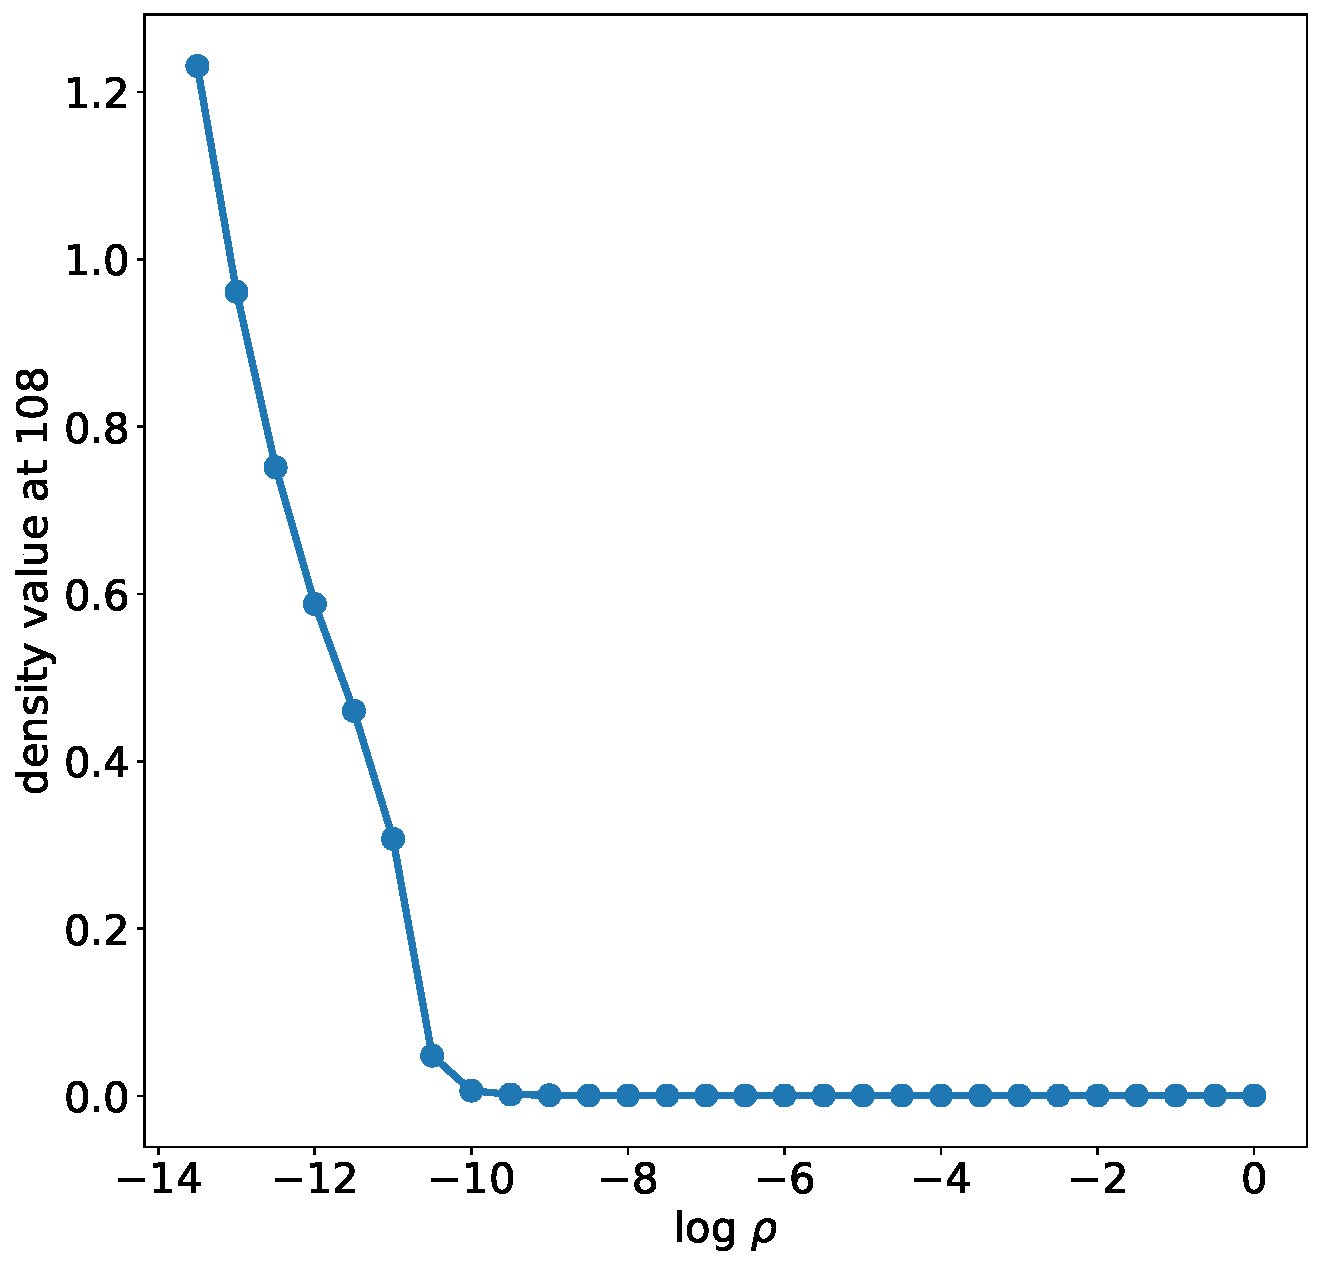
\includegraphics[width=0.6\textwidth]{../plots/density-at-108-vs-log-penalty-Gamma-36.0-2.0.pdf}
	\caption{Density value at $108$ against $\log \rho$.}
	\label{fig-density-val-108-vs-log-pen}
\end{figure}

%Density estimates in Figure \ref{fig-penalized-estimate} confirms our prediction. 
%
%\begin{figure}[t]
%	\centering
%	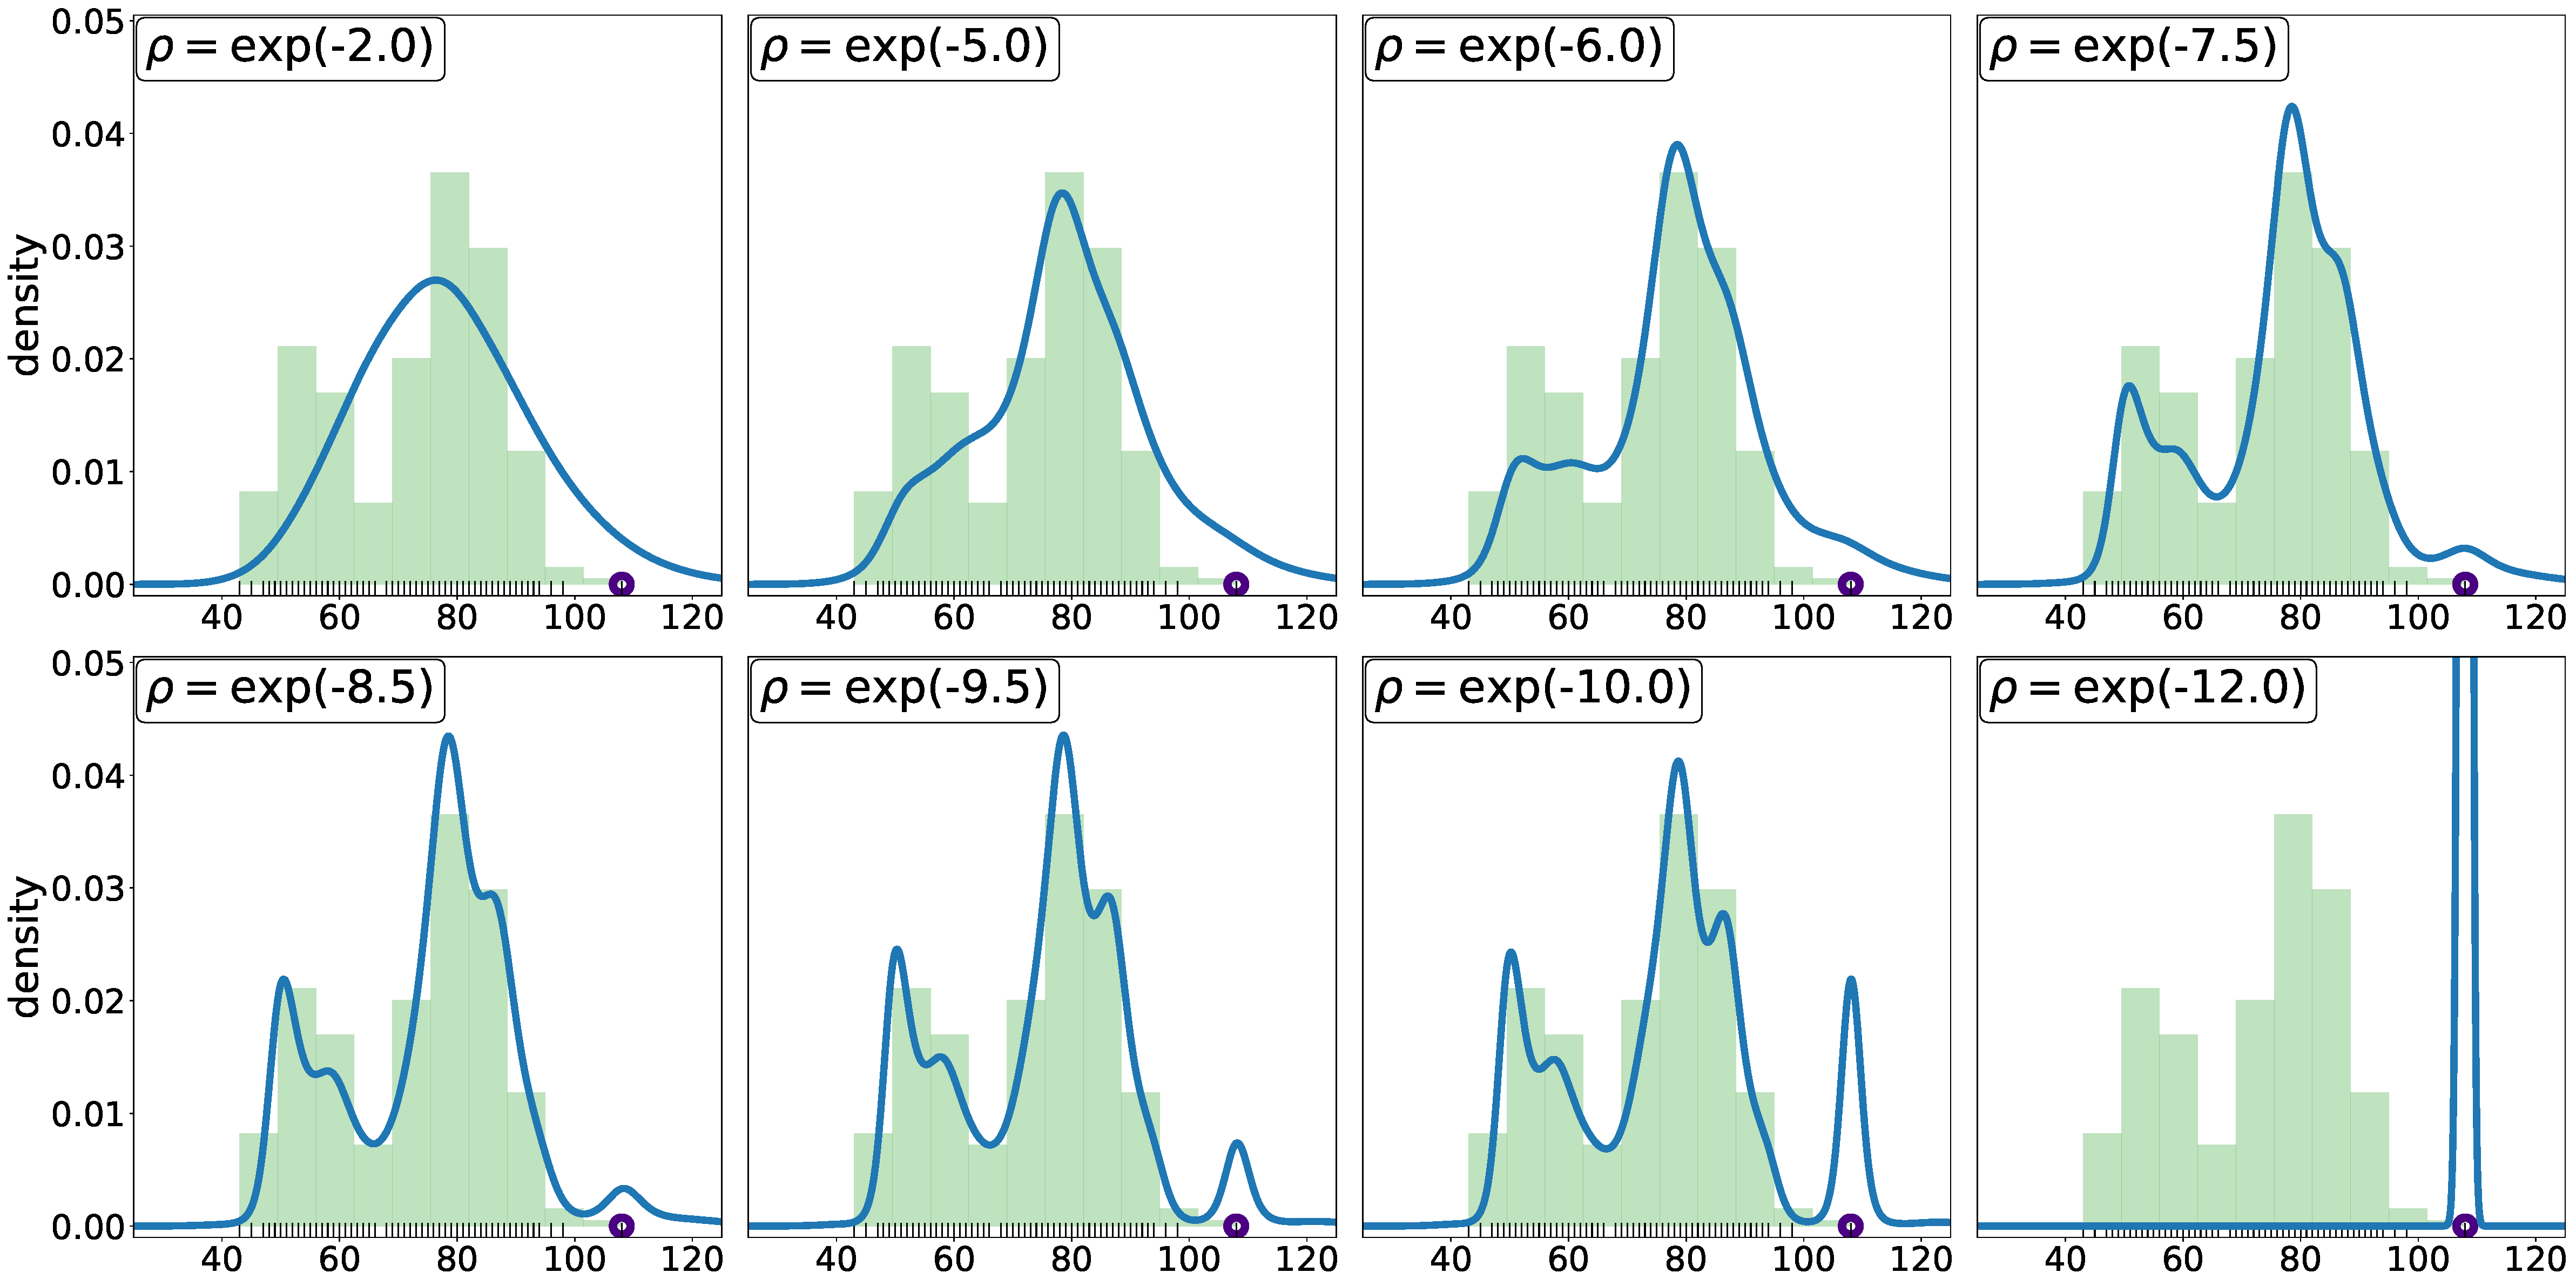
\includegraphics[width=\textwidth]{../plots/waiting-SM-density-estimates-penalized-only-bw=5.0-baseden=Gamma-26-3-entireRKHS.pdf}
%	\caption{Penalized SM density estimates for different values of penalty parameters labeled at the upper left corner. Histogram of data using the Freedman-Diaconis rule is shown in green. The rug plot indicates the location of data and the purple circle indicates the location of the observation 108.}
%	\label{fig-penalized-estimate}
%\end{figure}


\subsection{Comparison through Eigen-decomposition}

We show the similarities of the penalized and early stopping SM density estimators through their eigen-decomposition. 

To this end, we first observe that $\widehat{C}$ has finite rank, and must be a compact operator. In addition, it is self-adjoint. By the Hilbert-Schmidt theorem, there exists a set of eigenfunctions $\sets{\widehat{\psi}_{\nu}}_{\nu=1}^{R}$ that forms an orthonormal basis for $\range \parens{\widehat{C}}$ and $\widehat{C} \widehat{\psi}_{\nu} = \hat{\xi}_{\nu} \widehat{\psi}_{\nu}$ for all $\nu = 1, \cdots, R$, where $\hat{\xi}_1 \ge \hat{\xi}_2 \ge \cdots \ge \hat{\xi}_R > 0$ are the eigenvalues of $\widehat{C}$ and $R < \infty$ denotes the rank of $\widehat{C}$. 

By \eqref{eq-penalized-sm-sol} in Chapter \ref{ch2} and Proposition \ref{prop-commutativity-Pi}, we have 
\begin{align}
	\hat{f}^{\parens{\rho}} = \parens{\widehat{C} + \rho I}^{-1} \hat{z} = & \, \parens{\widehat{C} + \rho I}^{-1} \widehat{C} \hat{g}_1 + \frac{1}{\rho} \hat{z}_2 \nonumber \\ 
	= & \, \sum_{\nu=1}^R \frac{\hat{\xi}_{\nu}}{\hat{\xi}_{\nu} + \rho} \innerp{\hat{g}_1}{\widehat{\psi}_{\nu}}_{\calH} \widehat{\psi}_{\nu} + \frac{1}{\rho} \hat{z}_2, \label{eq-comparison-pen-es-1}
\end{align}
where $\hat{g}_1 \in \calH$ satisfying $\hat{z}_1 = \widehat{C} \hat{g}_1$. In addition, by Proposition \ref{prop-decomposition-ft}, we have 
\begin{align}
	\hat{f}^{\parens{t}} = \tau \sum_{j=0}^{t-1} \parens{I - \tau \widehat{C}}^j \hat{z} = & \, \parens{I - \parens{I - \tau \widehat{C}}^{t}} \hat{g}_1 + t \tau \hat{z}_2 \nonumber \\ 
	= & \, \sum_{\nu=1}^R \parens{1 - \parens{1 - \tau \hat{\xi}_{\nu} }^{t}} \innerp{\hat{g}_1}{\widehat{\psi}_{\nu}}_{\calH} \widehat{\psi}_{\nu} + t \tau \hat{z}_2. \label{eq-comparison-pen-es-2}
\end{align}
Comparing \eqref{eq-comparison-pen-es-1} and \eqref{eq-comparison-pen-es-2}, we see $\hat{f}^{\parens{\rho}}$ and $\hat{f}^{\parens{t}}$ are very similar. The main difference lies in how they regularize the eigenvalues $\sets{\hat{\xi}_{\nu}}_{\nu=1}^R$. In $\hat{f}^{\parens{\rho}}$, the regularization is done through the function $x \mapsto \frac{x}{x + \rho}$, and in $\hat{f}^{\parens{t}}$, the regularization is done through the function $x \mapsto 1 - \parens{1 - \tau x}^t$, for $x > 0$. 

For sufficiently small eigenvalues $\hat{\xi}_{\nu}$, $\frac{\hat{\xi}_{\nu}}{\hat{\xi}_{\nu} + \rho} \approx 0$ and $1 - \parens{1 - \tau \hat{\xi}_{\nu} }^{t} \approx 0$. Therefore, both of them attempt to attenuate the effects of the smaller eigenvalues and let the larger eigenvalues to dominate. 

\subsection{Comparison of Convergence Rates}

So far, we have been focusing more on the similarities of these two density estimators. We stress a key difference of them by examining their convergence rates. 

It has been shown in \textcite{Sriperumbudur-density-estimation-inf-exp-family} that, under the same assumptions as in Theorem \ref{theorem-convergence-rate}, we have $\norm{\hat{f}^{\parens{\rho}} - f_0}_{\calH} = \calO_{p_0} \parens{n^{-\min \braces[\big]{\frac{1}{4}, \frac{\gamma}{2 \parens{\gamma + 1}}}}}$. As the value of $\gamma$ is becoming large, the rate does \emph{not} improve with $\gamma$ and the best possible rate is $n^{-\frac{1}{4}}$, which is achieved when $\gamma = 1$. As we have discussed earlier, the value of $\gamma$ in \ref{assumption-7} indicates the degree of smoothness of $f_0$, and a larger value of $\gamma$ implies that $f_0$ is smoother. However, the rate of $\hat{f}^{\parens{\rho}}$ does \emph{not} really capture this smoothness, since, as soon as $\gamma$ exceeds 1, the rate stabilizes at $n^{-\frac{1}{4}}$ and never improves. This unsatisfactory feature of the penalized SM density estimator is 
%as it does \emph{not} exploit the smoothness of $f_0$. 
called the \emph{saturation phenomenon} in the literature, and has been the main motivation of designing new regularized estimators that do not saturate \parencite{Engl1996-jy,Bauer2007-xq,Lo_Gerfo2008-vv}. 

However, Theorem \ref{theorem-convergence-rate} implies that with the stopping rule $t^*$, we have $\norm{\hat{f}^{\parens{t^* \parens{n}}} - f_0}_{\calH} = \calO_{p_0} \parens{n^{-\frac{\gamma}{2 \parens{\gamma+2}}}}$. Note, in particular, that this rate improves as $\gamma$ increases. As $\gamma \to \infty$, this rate approaches to $n^{-\frac{1}{2}}$, which is faster compared to that in the penalized approach. 


\subsection{Numerical Examples}

We finally compare the early stopping and penalized SM density estimators numerically using the \texttt{waiting} variable in the Old Faithful Geyser dataset. 

The resulting penalized and early stopping SM density estimates with different choices of $\rho$ and $t$ are shown in Figure \ref{fig-earlystopping-pen-estimates}. It is obvious that these two approaches yield very similar density estimates: when the regularization is large (i.e., $\rho$ is large or $t$ is small), density estimates are very similar to $\mu$; as $\rho$ decreases or $t$ increases, density estimates become more reasonable and reveal the bimodal feature of data; if we further decrease $\rho$ or increase $t$ so that there is very small regularization, density estimates contain a bump or become a spike at the isolated observation 108. 

Additional numerical examples confirm our observations above. 

\begin{sidewaysfigure}
	\centering
	
\includegraphics[width=\textwidth]{../plots/waiting-SM-density-estimates-pen-vs-earlystopping-baseden=Gamma-36.0-2.0-entireRKHS-2.pdf}
	\caption{The penalized (first row) and early stopping (second row) SM density estimates with various choices of $\rho$ and $t$, respectively, shown at the upper left corner. Histogram of data with the bin width chosen by the Freedman-Diaconis rule is shown in green. The rug plot indicates the location of data and the purple circle indicates the location of the observation 108.}
	\label{fig-earlystopping-pen-estimates}
\end{sidewaysfigure}

\newpage

\section{Auxiliary Results and Proofs}

%\section{Solution to a Non-homogeneous Difference Equation}
%
%Throughout this section, we repeatedly used the following result on solving a difference equation. 
%
%\begin{proposition}\label{prop-solution-difference-equation}
%	Consider the following linear first-order difference equation
%	\begin{align}\label{eq-diff-equa}
%		x \parens{n+1} = a \parens{n} x \parens{n} + g \parens{n}, 
%	\end{align}
%	with the initial condition $x \parens{0} = x_0$, where we assume that $a \parens{n} \neq 0$ and that both $a \parens{n}$ and $g \parens{n}$ are real-valued functions defined for $n \in \Natural_0$. Then, the unique solution of \eqref{eq-diff-equa} is 
%	\begin{align}
%		x \parens{n+1} = \parens[\Bigg]{\prod_{i=0}^{n} a \parens{i}} x_0 + \sum_{j=0}^{n} \parens[\Bigg]{\prod_{i=j+1}^n a \parens{i}} g \parens{j}, 
%	\end{align}
%	where we let $\prod_{i=k+1}^k a \parens{i} = 1$ and $\sum_{i=k+1}^k a \parens{i} = 0$. 
%\end{proposition}
%
%The proof of Proposition \ref{prop-solution-difference-equation} is omitted but can be found, for example, in \textcite{Elaydi2013-ej}. The main idea of the proof is induction. 

\subsection{Proof of Theorem \ref{thm-grad-widehatJ}}\label{proof-thm-grad-widehatJ}

\begin{proof}[Proof of Theorem \ref{thm-grad-widehatJ}]
	In order to establish the desired result, we first show $\widehat{J}_{\SM}$ is Fr{\'e}chet differentiable over $\calH$ and derive its Frech{\'e}t derivative at $f \in \calH$, and then derive the Fr{\'e}chet gradient operator of $\widehat{J}_{\SM}$ using its definition. 
	
	Let $f \in \calH$ be arbitrary, and $g \in \calH$ be nonzero. 
%	By definition, $\widehat{J}_{\SM}$ is Fr{\'e}chet differentiable at $f \in \calH$ if there exists a bounded linear functional from $\calH$ to $\Real$ such that the following identity holds 
%	\begin{align}
%		\lim_{\norm{g}_{\calH} \to 0} \frac{\abs{\widehat{J}_{\SM} \parens{f + g} - \widehat{J}_{\SM} \parens{f} - \Diff \widehat{J}_{\SM} \parens{f} \parens{g}}}{\norm{g}_{\calH}} = 0, 
%	\end{align}
%	and this bounded linear operator $\Diff \widehat{J}_{\SM} \parens{f}$ is called the Fr{\'e}chet derivative. 
	It is easy to show $\widehat{C}$ is linear. Then, using its linearity, we have 
	\begin{align*}
		\widehat{J}_{\SM} \parens{f + g} - \widehat{J}_{\SM} \parens{f} 
		= & \, \parens[\bigg]{\frac{1}{2} \innerp{f + g}{\widehat{C} \parens{f + g}}_{\calH} - \innerp{f + g}{\hat{z}}_{\calH}} - \parens[\bigg]{\frac{1}{2} \innerp{f}{\widehat{C}f}_{\calH} - \innerp{f}{\hat{z}}_{\calH}} \\ 
		= & \, \innerp{g}{\widehat{C} f - \hat{z}} + \frac{1}{2} \innerp{g}{\widehat{C} g}_{\calH}. 
	\end{align*}
	It then follows 
	\begin{align*}
		0 \le & \, \frac{\abs[\big]{\widehat{J} \parens{f + g} - \widehat{J} \parens{f} - \innerp{g}{\widehat{C} f - \hat{z}}_{\calH}}}{\norm{g}_{\calH}} 
		= \frac{\abs{\frac{1}{2} \innerp{g}{\widehat{C} g}_{\calH}}}{\norm{g}_{\calH}} \\ 
		\stackrel{\mathrm{\parens{i}}}{\le} & \, \frac{1}{2} \norm[\big]{\widehat{C}g}_{\calH} 
		\stackrel{\text{(ii)}}{\le} \frac{1}{2n} \sum_{i=1}^n \sum_{u=1}^d \norm{\partial_u k \parens{X_i, \,\cdot\,}}_{\calH}^2 \norm{g}_{\calH} \\ 
		\stackrel{\text{(iii)}}{\le} & \, \frac{1}{2} d \kappa_2^2 \norm{g}_{\calH} \to 0, \qquad \text{ as } \norm{g}_{\calH} \to 0, 
	\end{align*}
	where we use the Cauchy-Schwartz inequality in (i), the triangle inequality and the Cauchy-Schwartz inequality in (ii), and \ref{assumption-5} in (iii). In addition, note the map $\Diff \widehat{J}_{\SM} \parens{f}: \calH \to \Real$ defined by $ \Diff \widehat{J}_{\SM} \parens{f} \parens{g} = \innerp{g}{\widehat{C}f - \hat{z}}_{\calH}$, for all $g \in \calH$, is linear and bounded, by \ref{assumption-5}. We conclude that $\widehat{J}_{\SM}$ is Frech{\'e}t differentiable at $f \in \calH$ with the Fr{\'e}chet derivative at $f \in \calH$ being 
	\begin{align*}
		\Diff \widehat{J}_{\SM} \parens{f} \parens{g} = \innerp{g}{\widehat{C}f - \hat{z}}_{\calH}, \qquad \text{ for all } g \in \calH. 
	\end{align*}
	Since our choice of $f \in \calH$ here is arbitrary, we conclude that $\widehat{J}_{\SM}$ is Frech{\'e}t differentiable over $\calH$. 
	
	Finally, by the definition of the Fr{\'e}chet gradient, we know $\nabla \widehat{J}_{\SM} \parens{f} = \widehat{C} f - \hat{z}$ for all $f \in \calH$. 
\end{proof}


\subsection{Proof of Theorem \ref{thm-closed-form}}\label{proof-thm-closed-form}

\begin{proof}[Proof of Theorem \ref{thm-closed-form}]
	We prove by induction. In the base case $t = 0$, it is straightforward from \eqref{eq-grad-updates} that 
	\begin{align}\label{eq-proof-thm3-1}
		\hat{f}^{\parens{1}} = & \, \hat{f}^{\parens{0}} - \tau_0 \parens{\widehat{C} \hat{f}^{\parens{0}} - \hat{z}} = \parens{I - \tau_0 \widehat{C}} \hat{f}_{0} + \tau_0 \hat{z}. 
	\end{align}
	Setting $t=0$ in \eqref{eq-closed-form} yields
	\begin{align*}
		\hat{f}^{\parens{1}} = & \, \prod_{i=0}^0 \parens{I - \tau_i \widehat{C}} \hat{f}^{\parens{0}} + \sum_{j=0}^0 \bracks[\Bigg]{\prod_{i=j+1}^0 \parens{I - \tau_i \widehat{C}}} \tau_j \hat{z} 
		= \parens{I - \tau_0 \widehat{C}} \hat{f}^{\parens{0}} + \tau_0 \hat{z}, 
	\end{align*}
	which matches \eqref{eq-proof-thm3-1}. 
	
	Now, we assume \eqref{eq-closed-form} holds for $t = s$ for some $s \in \Natural$, and we wish to show that it also holds for $t = s+1$. By \eqref{eq-grad-updates}, we know that $\hat{f}^{\parens{s+1}} = \parens{I - \tau_s \widehat{C}} \hat{f}^{\parens{s}} + \tau_s \hat{z}$, and by the inductive hypothesis, we know that $\hat{f}^{\parens{s}} = \prod_{i=0}^{s-1} \parens{I - \tau_i \widehat{C}} \hat{f}^{\parens{0}} + \sum_{j=0}^{s-1} \bracks[\big]{\prod_{i=j+1}^{s-1} \parens{I - \tau_i \widehat{C}}} \tau_j \hat{z}$. Hence, 
	\begin{align*}
		\hat{f}^{\parens{s+1}} % = & \, \parens{I - \tau_k \widehat{C}} \hat{f}^{\parens{s}} + \tau_s \hat{z} \\ 
		= & \, \parens{I - \tau_s \widehat{C}} \bracks[\Bigg]{\prod_{i=0}^{s-1} \parens{I - \tau_i \widehat{C}} \hat{f}^{\parens{0}} + \sum_{j=0}^{s-1} \parens[\Bigg]{\prod_{i=j+1}^{s-1} \parens{I - \tau_i \widehat{C}}} \tau_j \hat{z}} + \tau_s \hat{z} \\ 
		= & \, \prod_{i=0}^{s} \parens{I - \tau_i \widehat{C}} \hat{f}^{\parens{0}} + \sum_{j=0}^{s-1} \prod_{i=j+1}^{s} \parens{I - \tau_i \widehat{C}} \tau_j \hat{z} + \prod_{i=s+1}^s \parens{I - \tau_i \widehat{C}} \tau_s \hat{z} \\ 
		= & \, \prod_{i=0}^{s} \parens{I - \tau_i \widehat{C}} \hat{f}^{\parens{0}} + \sum_{j=0}^{s} \parens[\Bigg]{\prod_{i=j+1}^{s} \parens{I - \tau_i \widehat{C}}} \tau_j \hat{z},  
	\end{align*}
	which is the desired result. 
	
	The case of the constant step size is straightforward. 
\end{proof}


\subsection{Proof of Theorem \ref{thm-early-stopping-algo}}\label{proof-theorem-early-stopping-algo}

In order to prove Theorem \ref{thm-early-stopping-algo}, we need the following lemma, which is essentially a generalized version of the binomial theorem with elements in a Hilbert space. 

\begin{lemma}\label{lemma-binomial-C}
	For all $j \in \Natural_0$, we have 
	\begin{align}\label{eq-lemma-bonimial-C-1}
		\parens{I - \tau \widehat{C}}^j = \sum_{\ell=0}^j {j \choose \ell} \parens{-\tau}^{\ell} \widehat{C}^{\ell}. 
	\end{align}
\end{lemma}

\begin{proof}[Proof of Lemma \ref{lemma-binomial-C}]
	We prove by induction. When $j = 0$, the left-hand side of \eqref{eq-lemma-bonimial-C-1} is simply $\parens{I - \tau \widehat{C}}^0 = I$, and the right-hand side is 
	\begin{align*}
		\sum_{\ell=0}^0 {j \choose \ell} \parens{-\tau}^{\ell} \widehat{C}^{\ell} = {0 \choose 0} \parens{-\tau}^{0} \widehat{C}^{0} = I. 
	\end{align*}
	Hence, \eqref{eq-lemma-bonimial-C-1} holds for $j = 0$. 
	
	Now, we assume \eqref{eq-lemma-bonimial-C-1} holds for $j = s$, and we show it also holds for $j = s + 1$. With $j = s+1$, the left-hand side of \eqref{eq-lemma-bonimial-C-1} becomes 
	\begin{align*}
		\parens{I - \tau \widehat{C}}^{s+1} = & \, \parens{I - \tau \widehat{C}} \parens{I - \tau \widehat{C}}^{s} \\ 
		= & \, \parens{I - \tau \widehat{C}} \bracks[\Bigg]{\sum_{\ell=0}^s {s \choose \ell} \parens{-\tau}^{\ell} \widehat{C}^{\ell} } \\ 
		= & \, I \bracks[\Bigg]{\sum_{\ell=0}^s {s \choose \ell} \parens{-\tau}^{\ell} \widehat{C}^{\ell} } - \tau \widehat{C} \bracks[\Bigg]{\sum_{\ell=0}^s {s \choose \ell} \parens{-\tau}^{\ell} \widehat{C}^{\ell} } \\ 
		= & \, \sum_{\ell=0}^s {s \choose \ell} \parens{-\tau}^{\ell} \widehat{C}^{\ell} + \sum_{\ell=0}^s {s \choose \ell} \parens{-\tau}^{\ell + 1} \widehat{C}^{\ell + 1} \\ 
		= & \, I + \sum_{\ell=1}^s {s \choose \ell} \parens{-\tau}^{\ell} \widehat{C}^{\ell} + \sum_{\ell=0}^{s-1} {s \choose \ell} \parens{-\tau}^{\ell + 1} \widehat{C}^{\ell + 1} + {s \choose s} \parens{-\tau}^{s+1} \widehat{C}^{s + 1} \\ 
		= & \, I + \sum_{\ell=1}^s {s \choose \ell} \parens{-\tau}^{\ell} \widehat{C}^{\ell} + \sum_{\ell=1}^{s} {s \choose \ell-1} \parens{-\tau}^{\ell} \widehat{C}^{\ell} + \parens{-\tau}^{s+1} \widehat{C}^{s + 1} \\ 
		= & \, I + \sum_{\ell=1}^s \bracks[\bigg]{{s \choose \ell} + {s \choose \ell-1}} \parens{-\tau}^{\ell} \widehat{C}^{\ell} + \parens{-\tau}^{s+1} \widehat{C}^{s + 1} \\ 
		= & \, {s+1 \choose 0} I + \sum_{\ell=1}^s {s+1 \choose \ell} \parens{-\tau}^{\ell} \widehat{C}^{\ell} + {s+1 \choose s+1} \parens{-\tau}^{s+1} \widehat{C}^{s + 1} \\ 
		= & \, \sum_{\ell=0}^{s+1} {s+1 \choose \ell} \parens{-\tau}^{\ell} \widehat{C}^{\ell}, 
	\end{align*}
	where we use the inductive hypothesis in the second equality. 
\end{proof}


We also need the following lemma which gives an explicit characterization of $\widehat{C}^{\ell} \hat{z}$. 

\begin{lemma}\label{lemma-C-power-z}
	For all $\ell \in \Natural$, we have 
	\begin{align}\label{eq-C-power-z}
		\widehat{C}^{\ell} \hat{z} = \frac{1}{n^{\ell}} \sum_{i=1}^n \sum_{u=1}^d \bracks[\big]{\bG^{\ell-1} \bh}_{\parens{i-1}d+u} \partial_u k \parens{X_i, \,\cdot\,}, 
	\end{align}
	where $\bG \in \Real^{nd \times nd}$ and $\bh \in \Real^{nd}$ are the same as those defined in Theorem \ref{thm-early-stopping-algo}. 
%	the $\parens{\parens{i-1}d+u, \parens{j-1}d+v}$-th entry of $\bG \in \Real^{\parens{nd} \times \parens{nd}}$ is $\innerp{\partial_u k \parens{X_i, \cdot}}{\partial_v k \parens{X_j, \cdot}}_{\calH} = \partial_u \partial_{v+d} k \parens{X_i, X_j}$, and the $\parens{\parens{i-1}d+u}$-th entry of $\bh \in \Real^{nd}$ is 
%	\begin{align*}
%		\innerp{\hat{z}}{\partial_u k \parens{X_i, \,\cdot\,}}_{\calH} = - \frac{1}{n} \sum_{j=1}^n \sum_{v=1}^d \parens[\Big]{\partial_u \partial^2_{v+d} k \parens{X_i, X_j} + \partial_v \log \mu \parens{X_j} \partial_u \partial_{v+d} k \parens{X_i, X_j}}. 
%	\end{align*}
\end{lemma}


\begin{proof}[Proof of Lemma \ref{lemma-C-power-z}]
	First note that, for any $\ell \ge 1$, $\widehat{C}^{\ell} \hat{z}$ resides in $\range \parens{\widehat{C}}$ that contains all functions of the form 
	\begin{align*}
		\widehat{C} g = \frac{1}{n} \sum_{i=1}^n \sum_{u=1}^d \innerp{\partial_u k \parens{X_i, \,\cdot\,}}{g}_{\calH} \partial_u k \parens{X_i, \,\cdot\,}, \qquad \text{ for some } g \in \calH. 
	\end{align*}	
	In other words, all functions in $\range \parens{\widehat{C}}$ can be written as a linear combination of $\partial_u k \parens{X_i, \,\cdot\,}$, for all $i = 1, \cdots, n$ and $u = 1, \cdots, d$. 
	
	We prove \eqref{eq-C-power-z} by induction. Note when $\ell = 1$, the left-hand side of \eqref{eq-C-power-z} is 
	\begin{align*}
		\widehat{C} \hat{z} = & \, \frac{1}{n} \sum_{i=1}^n \sum_{u=1}^d \innerp{\partial_u k \parens{X_i, \,\cdot\,}}{\hat{z}}_{\calH} \partial_u k \parens{X_i, \,\cdot\,} 
		= \frac{1}{n} \sum_{i=1}^n \sum_{u=1}^d \bracks{\bh}_{\parens{i-1}d+u} \partial_u k \parens{X_i, \,\cdot\,} \\ 
		= & \, \frac{1}{n} \sum_{i=1}^n \sum_{u=1}^d \bracks{\bG^{1-1} \bh}_{\parens{i-1}d+u} \partial_u k \parens{X_i, \,\cdot\,}. 
	\end{align*}
	Hence, \eqref{eq-C-power-z} holds for $\ell = 1$. 
	
	Now, suppose that \eqref{eq-C-power-z} holds for $\ell = s$. We want to show it also holds for $\ell = s + 1$. Note the following 
	\begin{align*}
		\widehat{C}^{s+1} \hat{z} = & \, \widehat{C} \parens{\widehat{C}^{s} \hat{z}} \\ 
		= & \, \parens[\bigg]{\frac{1}{n} \sum_{i=1}^n \sum_{u=1}^d \partial_u k \parens{X_i, \,\cdot\,} \otimes \partial_u k\parens{X_i, \,\cdot\,}} \parens[\bigg]{\frac{1}{n^{s}} \sum_{j=1}^n \sum_{v=1}^d \bracks{\bG^{s-1} \bh}_{\parens{j-1}d+v} \partial_v k \parens{X_j, \,\cdot\,}} \\ 
		= & \, \frac{1}{n^{s+1}} \sum_{i=1}^n \sum_{u=1}^d \parens[\bigg]{\sum_{j=1}^n \sum_{v=1}^d \bracks{\bG^{s-1} \bh}_{\parens{j-1}d+v} \innerp{\partial_u k \parens{X_i, \,\cdot\,}}{\partial_v k\parens{X_j, \,\cdot\,}}_{\calH}} \partial_u k \parens{X_i, \,\cdot\,} \\ 
		= & \, \frac{1}{n^{s+1}} \sum_{i=1}^n \sum_{u=1}^d \parens[\bigg]{\sum_{j=1}^n \sum_{v=1}^d \bracks{\bG^{s-1} \bh}_{\parens{j-1}d+v} \partial_u \partial_v k \parens{X_i, X_j}} \partial_u k \parens{X_i, \,\cdot\,} \\ 
		= & \, \frac{1}{n^{s+1}} \sum_{i=1}^n \sum_{u=1}^d \bracks{\bG^{s} \bh}_{\parens{i-1}d+u} \partial_u k \parens{X_i, \,\cdot\,}, 
	\end{align*}
	which is the desired result. 
\end{proof}

We now prove Theorem \ref{thm-early-stopping-algo}. 

\begin{proof}[Proof of Theorem \ref{thm-early-stopping-algo}]
	Since, for $t \in \Natural_0$, we have $\hat{f}^{\parens{t+1}} = \tau \sum_{j=0}^t \parens{I - \tau \widehat{C}}^{j} \hat{z}$, using the results of Lemma \ref{lemma-binomial-C}, we can rewrite it as 
	\begin{align*}
		\hat{f}^{\parens{t+1}} = & \, \tau \sum_{j=0}^t \sum_{\ell=0}^j {j \choose \ell} \parens{-\tau}^{\ell} \widehat{C}^{\ell} \hat{z} \nonumber \\ 
		= & \, \tau \hat{z} + \tau \sum_{j=1}^t \sum_{\ell=0}^j {j \choose \ell} \parens{-\tau}^{\ell} \widehat{C}^{\ell} \hat{z} \nonumber \\ 
		= & \, \tau \hat{z} + \tau \sum_{j=1}^t \bracks[\bigg]{\hat{z} + \sum_{\ell=1}^j {j \choose \ell} \parens{-\tau}^{\ell} \widehat{C}^{\ell} \hat{z}} \nonumber \\ 
		= & \, \tau \parens{t + 1} \hat{z} + \tau \sum_{j=1}^t \sum_{\ell=1}^j {j \choose \ell} \parens{-\tau}^{\ell} \widehat{C}^{\ell} \hat{z}. % \label{eq-ft-iter}
	\end{align*}
	Using Lemma \ref{lemma-C-power-z}, we have 
	\begin{align*}
		\hat{f}^{\parens{t+1}} = & \, \tau \parens{t + 1} \hat{z} + \tau \sum_{j=1}^t \sum_{\ell=1}^j {j \choose \ell} \parens{-\tau}^{\ell} \bracks[\bigg]{\frac{1}{n^{\ell}} \sum_{i=1}^n \sum_{u=1}^d \bracks{\bG^{\ell-1} \bh}_{\parens{i-1}d+u} \partial_u k \parens{X_i, \,\cdot\,}} \nonumber \\ 
		= & \, \tau \parens{t + 1} \hat{z} + \tau \sum_{i=1}^n \sum_{u=1}^d \bracks[\Bigg]{\sum_{j=1}^t \sum_{\ell=1}^j {j \choose \ell} \parens[\bigg]{\frac{\parens{-\tau}^{\ell}}{n^{\ell}} \bG^{\ell-1} \bh}}_{\parens{i-1}d+u} \partial_u k \parens{X_i, \,\cdot\,}. 
	\end{align*}
	This proves \eqref{eq-thm-early-stopping-algo-part1}. 
	
	To prove \eqref{eq-thm-early-stopping-algo-part2}, first note the matrix $\bG$ is the Gram matrix of the set of vectors $\sets{\partial_u k \parens{X_i, \,\cdot\,} \text{ for } i = 1, \cdots, n \text{ and } u = 1, \cdots, d}$, implying that $\bG$ is positive semi-definite. Hence, we can write $\bG = \bQ \bLambda \bQ^{\top}$, where again $\bQ \in \Real^{nd \times nd}$ is an orthogonal matrix and $\bLambda \in \Real^{nd \times nd}$ is a diagonal matrix with the eigenvalues of $\bG$, $\lambda_1 \ge \lambda_2 \ge \cdots \ge \lambda_{nd} \ge 0$, on the diagonal. Hence, 
	\begin{align}
		\sum_{j=1}^t \sum_{\ell=1}^j {j \choose \ell} \parens[\bigg]{\frac{\parens{-\tau}^{\ell}}{n^{\ell}} \bG^{\ell-1} \bh}  \nonumber
		= & \, - \frac{\tau}{n} \sum_{j=1}^t \sum_{\ell=1}^j {j \choose \ell} \parens[\bigg]{\parens[\bigg]{- \frac{\tau}{n}}^{\ell-1} \parens{\bQ \bLambda \bQ^\top}^{\ell-1} \bh} \nonumber \\ 
		= & \, - \frac{\tau}{n} \sum_{j=1}^t \sum_{\ell=1}^j {j \choose \ell} \parens[\bigg]{\parens[\bigg]{- \frac{\tau}{n}}^{\ell-1} \bQ \bLambda^{\ell-1} \bQ^\top \bh} \nonumber \\ 
		= & \, - \frac{\tau}{n} \bQ \bracks[\Bigg]{\sum_{j=1}^t \sum_{\ell=1}^j {j \choose \ell} \parens[\bigg]{- \frac{\tau}{n} \bLambda}^{\ell-1}} \bQ^\top \bh. \label{ft.iter1}
	\end{align}
	Now, since $\bLambda$ is a diagonal matrix, the sum and the power in \eqref{ft.iter1} can be performed only on the diagonal elements. Since, by the binomial theorem, 
	\begin{align*}
		\parens{1 + x}^j = 1 + \sum_{\ell=1}^j {j \choose \ell} x^{\ell}, \qquad \quad \text{ for all } x \in \Real, 
	\end{align*}
	we have, for all $w = 1, \cdots, nd$, if $\lambda_w \neq 0$, 
	\begin{align*}
		\sum_{j=1}^t \sum_{\ell=1}^j {j \choose \ell} \parens[\bigg]{- \frac{\tau}{n} \lambda_{w}}^{\ell-1} = & \, \parens[\bigg]{- \frac{\tau}{n} \lambda_{w}}^{-1} \sum_{j=1}^t \bracks[\Bigg]{\sum_{\ell=1}^j {j \choose \ell} \parens[\bigg]{- \frac{\tau}{n} \lambda_{w}}^{\ell}} \nonumber \\ 
		= & \, \parens[\bigg]{- \frac{\tau}{n} \lambda_{w}}^{-1} \sum_{j=1}^t \bracks[\Bigg]{\parens[\bigg]{1 - \frac{\tau}{n} \lambda_{w}}^j - 1} \nonumber \\ 
		= & \, \parens[\bigg]{- \frac{\tau}{n} \lambda_{w}}^{-1} \parens[\bigg]{1 - \frac{\tau}{n} \lambda_{w}} \frac{1 - \parens[\big]{1 - \frac{\tau}{n} \lambda_{w}}^t}{1 - \parens[\big]{1 - \frac{\tau}{n} \lambda_{w}}} - t \parens[\bigg]{- \frac{\tau}{n} \lambda_{w}}^{-1} \nonumber \\ 
		= & \, - \parens[\bigg]{\frac{n}{\tau \lambda_w}}^{2} \parens[\bigg]{1 - \frac{\tau}{n} \lambda_{w}} \parens[\bigg]{1 - \parens[\Big]{1 - \frac{\tau}{n} \lambda_{w}}^t} + \frac{tn}{\tau \lambda_w}, % \label{power.sum.lambda1}
	\end{align*}
	and, if $\lambda_w = 0$, we have 
	\begin{align*}
		\sum_{j=1}^t \sum_{\ell=1}^j {j \choose \ell} \parens[\bigg]{- \frac{\tau}{n} \lambda_{w}}^{\ell-1} = \sum_{j=1}^t j = \frac{\parens{t+1} t}{2}, % \label{power.sum.lambda2}
	\end{align*}
	which are exactly the diagonal elements of $\widetilde{\bLambda}$ defined in the theorem. Therefore, we have 
	\begin{align*}
		\sum_{j=1}^t \sum_{\ell=1}^j {j \choose \ell} \parens[\bigg]{\frac{\parens{-\tau}^{\ell}}{n^{\ell}} \bG^{\ell-1} \bh} = - \frac{\tau}{n} \bQ \widetilde{\bLambda} \bQ^\top \bh, 
	\end{align*}
	
	In addition, we have 
	\begin{align*}
		\hat{f}^{\parens{t+1}} = & \, \tau \parens{t + 1} \hat{z} + \tau \sum_{i=1}^n \sum_{u=1}^d \bracks[\Bigg]{- \frac{\tau}{n} \bQ \widetilde{\bLambda} \bQ^\top \bh}_{\parens{i-1}d+u} \partial_u k \parens{X_i, \,\cdot\,} \\ 
		= & \, \tau \parens{t + 1} \hat{z} - \frac{\tau^2}{n} \sum_{i=1}^n \sum_{u=1}^d \bracks[\Big]{\bQ \widetilde{\bLambda} \bQ^\top \bh}_{\parens{i-1}d+u} \partial_u k \parens{X_i, \,\cdot\,}, 
	\end{align*}
	which completes the proof. 
\end{proof}


\subsection{Proofs of Results in Section \ref{subsec-smes-limiting-t}}\label{subsection-proof-smes-limiting-t}

\begin{proof}[Proof of Proposition \ref{prop-decomposition-ft}]
	Since we can write $\hat{z} = \hat{z}_1 + \hat{z}_2$ with $\hat{z}_1 = \widehat{C} \hat{g}_1 \in \range \parens{\widehat{C}}$ and $\hat{z}_2 \in \range \parens{\widehat{C}}^{\perp}$, we can write the $\parens{t+1}$-st gradient descent iterate as 
	\begin{align*}
		\hat{f}^{\parens{t+1}} = \parens{I - \tau \widehat{C}} \hat{f}^{\parens{t}} + \tau \parens{\hat{z}_1 + \hat{z}_2} = \parens{I - \tau \widehat{C}} \hat{f}^{\parens{t}} + \tau \widehat{C} \hat{g}_1 + \tau \hat{z}_2. 
	\end{align*}
	Subtracting both sides of the preceding equation by $\hat{g}_1$ yields 
	\begin{align}
		\hat{f}^{\parens{t+1}} - \hat{g}_1 %= & \, \parens{I - \tau \widehat{C}} \hat{f}^{\parens{t}} - \hat{g}_1 + \tau \widehat{C} \hat{g}_1 + \tau \hat{z}_2 \nonumber \\ 
		= & \, \parens{I - \tau \widehat{C}} \parens{\hat{f}^{\parens{t}} - \hat{g}_1} + \tau \hat{z}_2. \label{eq-proof-prop-decomposition-ft-1}
	\end{align}
	Projecting both sides of \eqref{eq-proof-prop-decomposition-ft-1} onto $\range \parens{\widehat{C}}$, we obtain 
	\begin{align*}
		\Pi_{\range \parens{\widehat{C}}} \parens{\hat{f}^{\parens{t+1}} - \hat{g}_1} = & \, \Pi_{\range \parens{\widehat{C}}} \parens[\big]{ \parens{I - \tau \widehat{C}} \parens{\hat{f}^{\parens{t}} - \hat{g}_1} + \tau \hat{z}_2} \nonumber \\
		= & \, \parens{I - \tau \widehat{C}} \Pi_{\range \parens{\widehat{C}}} \parens{\hat{f}^{\parens{t}} - \hat{g}_1} \\ 
		= & \, \parens{I - \tau \widehat{C}}^{t+1} \Pi_{\range \parens{\widehat{C}}} \parens{\hat{f}^{\parens{0}} - \hat{g}_1} \\ 
		= & \, \parens{I - \tau \widehat{C}}^{t+1} \Pi_{\range \parens{\widehat{C}}} \parens{- \hat{g}_1} \\ 
		= & \, - \parens{I - \tau \widehat{C}}^{t+1} \hat{g}_1, 
	\end{align*}
	where we use $\hat{f}^{\parens{0}} = 0$ in the next to last equality and $\hat{g}_1 \in \range \parens{\widehat{C}}$ to obtain the last equality. 
	
	Now, project both sides of \eqref{eq-proof-prop-decomposition-ft-1} onto $\range \parens{\widehat{C}}^{\perp}$, we obtain 
	\begin{align*}
		\Pi_{\range \parens{\widehat{C}}^{\perp}} \parens{\hat{f}^{\parens{t+1}} - \hat{g}_1} = & \, \Pi_{\range \parens{\widehat{C}}^{\perp}} \parens{\hat{f}^{\parens{t}} - \hat{g}_1} + \tau \hat{z}_2 \\ 
		= & \, \Pi_{\range \parens{\widehat{C}}^{\perp}} \parens{\hat{f}^{\parens{0}} - \hat{g}_1} + \parens{t+1} \tau \hat{z}_2 \\
		= & \, \parens{t+1} \tau \hat{z}_2, 
	\end{align*}
	where we again use $\hat{f}^{\parens{0}} = 0$ and $\hat{g}_1 \in \range \parens{\widehat{C}}$. 
	
	Finally, we have 
	\begin{align*}
		\hat{f}^{\parens{t+1}} = & \, \hat{g}_1 + \Pi_{\range \parens{\widehat{C}}} \parens{\hat{f}^{\parens{t+1}} - \hat{g}_1} + \Pi_{\range \parens{\widehat{C}}^{\perp}} \parens{\hat{f}^{\parens{t+1}} - \hat{g}_1} \nonumber \\ 
		= & \, \hat{g}_1 - \parens{I - \tau \widehat{C}}^{t+1} \hat{g}_1 + \tau \parens{t+1} \hat{z}_2 \nonumber \\ 
		= & \, \parens{I - \parens{I - \tau \widehat{C}}^{t+1}} \hat{g}_1 + \tau \parens{t+1} \hat{z}_2, 
	\end{align*}
	which is the desired result. 
\end{proof}


\begin{proof}[Proof of Proposition \ref{prop-hatz1-hatz2-g1}]
	\ref{prop-hatz1-hatz2-g1-1} Since $\hat{z}_1$ is the orthogonal projection of $\hat{z}$ onto $\range \parens{\widehat{C}}$, by the definition of projection, we have 
		\begin{align*}
			\hat{z}_1 = \argmin_{w \in \range \parens{\widehat{C}}} \norm{\hat{z} - w}_{\calH}^2. 
		\end{align*}
	Since $w \in \range \parens{\widehat{C}}$, we can write $w = \sum_{i=1}^n \sum_{u=1}^d \alpha_{\parens{i-1}d+u} \partial_u k \parens{X_i, \,\cdot\,}$ for some $\balpha := \parens{\alpha_{1}, \cdots, \alpha_{nd}}^\top \in \Real^{nd}$. Then, 
	\begin{align*}
		\norm{\hat{z} - w}_{\calH}^2 = & \, \norm[\bigg]{\hat{z} - \sum_{i=1}^n \sum_{u=1}^d \alpha_{\parens{i-1}d+u} \partial_u k \parens{X_i, \,\cdot\,}}_{\calH}^2 \nonumber \\ 
		= & \, \norm{\hat{z}}_{\calH}^2 - 2 \sum_{i=1}^n \sum_{u=1}^d  \alpha_{\parens{i-1}d+u} \innerp{\hat{z}}{ \partial_u k \parens{X_i, \,\cdot\,} }_{\calH} + \norm[\Bigg]{\sum_{i=1}^n \sum_{u=1}^d \alpha_{\parens{i-1}d+u} \partial_u k \parens{X_i, \,\cdot\,}}_{\hil}^2 \nonumber \\ 
		= & \, \norm{\hat{z}}_{\calH}^2 - 2 \balpha^\top \bh + \balpha^\top \bG \balpha. 
	\end{align*}
	Since $\bG$ is a Gram matrix and is positive definite by assumption, the function $\balpha \mapsto \norm{\hat{z}}_{\calH}^2 - 2 \balpha^\top \bh + \balpha^\top \bG \balpha$ is convex and differentiable in $\balpha$. Then, $\balpha^* := \argmin_{\balpha} \sets{\norm{\hat{z}}_{\calH}^2 - 2 \balpha^\top \bh + \balpha^\top \bG \balpha}$ must exist and satisfy the first-order optimality condition $\boldzero = - \bh + \bG \balpha^*$, which is the desired linear system. 

	% If, in particular, $\bG \in \Real^{nd \times nd}$ is invertible, $\balpha^* = \bG^{-1} \bh$. 
		
	\ref{prop-hatz1-hatz2-g1-2} The result is straightforward using the relationship $\hat{z} = \hat{z}_1 + \hat{z}_2$, the definition of $\hat{z}$, the result from \ref{prop-hatz1-hatz2-g1-1}. 
	
	\ref{prop-hatz1-hatz2-g1-3} Since $\hat{g}_1$ belongs to $\range \parens{\widehat{C}}$ and satisfies the relationship $\hat{z}_1 = \widehat{C} \hat{g}_1$, we let $\hat{g}_1 = \sum_{j=1}^n \sum_{v=1}^d \beta_{\parens{j-1}d+v}^* \partial_j k \parens{X_b, \,\cdot\,}$ and must have 
	\begin{align*}
		\hat{z}_1 = \widehat{C} \hat{g}_1 = & \, \bracks[\Bigg]{\frac{1}{n} \sum_{i=1}^n \sum_{u=1}^d \partial_u k \parens{X_i, \,\cdot\,} \otimes \partial_u k \parens{X_i, \,\cdot\,}} \parens[\Bigg]{\sum_{j=1}^n \sum_{v=1}^d \beta_{\parens{j-1}d+v}^* \partial_v k \parens{X_j, \,\cdot\,}} \nonumber \\ 
		= & \, \sum_{i=1}^n \sum_{u=1}^d \bracks[\Bigg]{ \frac{1}{n} \sum_{j=1}^n \sum_{v=1}^d \beta_{\parens{j-1}d+v}^* \partial_u \partial_{v+d} k \parens{X_i, X_j}} \partial_u k \parens{X_i, \,\cdot\,}. 
	\end{align*}
	It follows that, for all $i = 1, \cdots, n$ and $u = 1, \cdots, d$, 
	\begin{align*}
		\alpha^*_{\parens{i-1}d+u} = \frac{1}{n} \sum_{j=1}^n \sum_{v=1}^d \beta_{\parens{j-1}d+v}^* \partial_u \partial_{v+d} k \parens{X_i, X_j}. 
	\end{align*}
	In other words, $\bbeta^* := \parens{\beta_1^*, \cdots, \beta_{nd}^*}^\top \in \Real^{nd}$ must satisfy $\frac{1}{n} \bG \bbeta^* = \balpha^*$. 
\end{proof}


\begin{proof}[Proof of Proposition \ref{proposition-bound-hatz1}]
	Recall from Proposition \ref{prop-decomposition-ft} that $\hat{f}_1^{\parens{t+1}} = \parens{I - \parens{I - \tau \widehat{C}}^t} \hat{g}_1$. Then, note the following 
	\begin{align*}
		\abs{\innerp{\hat{f}_1^{\parens{t+1}}}{k \parens{x, \,\cdot\,}}_{\calH}} = & \, \abs[\big]{\innerp{\parens{I - \parens{I - \tau \widehat{C}}^t} \hat{g}_1}{k \parens{x, \,\cdot\,}}_{\calH}} \\ 
		\stackrel{\text{(i)}}{\le} & \, \norm{I - \parens{I - \tau \widehat{C}}^t} \norm{\hat{g}_1}_{\calH} \norm{k \parens{x, \,\cdot\,}}_{\calH} \\ 
		 \stackrel{\text{(ii)}}{\le} & \, \norm{\hat{g}_1}_{\calH} \sup_{x \in \calX} \norm{k \parens{x, \,\cdot\,}}_{\calH} \\ 
		 \stackrel{\text{(iii)}}{\le} & \, \kappa_1 \norm{\hat{g}_1} =: M. 
	\end{align*}
	In the development above, (i) follows from the Cauchy-Schwartz inequality and the sub-multiplicative property and the definition of the operator norm. Due to \ref{assumption-limiting-2}, $\norm{I - \parens{I - \tau \widehat{C}}^t} \le 1$ for all $t$ and (ii) holds. Finally, (iii) follows from \ref{assumption-2-2-bdd-kernel}. 
\end{proof}

We are now ready to prove Theorem \ref{thm-limiting-density-t}. 

\begin{proof}[Proof of Theorem \ref{thm-limiting-density-t}]
	Let $\hat{z}_2 \parens{x} := \innerp{\hat{z}_2}{ k \parens{x, \,\cdot\,}}_{\calH}$ for all $x \in \calX$. Notice that
	\begin{align*}
		q_{\hat{f}^{\parens{t}}} \parens{x^*} = \frac{\mu \parens{x^*} \exp \parens[\big]{\innerp{\parens{I - \parens{I - \tau \widehat{C}}^t} \hat{g}_1}{k \parens{x^*, \,\cdot\,}}_{\calH} + \tau t \hat{z}_2 \parens{x^*}}}{\int_{\calX} \mu \parens{x} \exp \parens[\big]{\innerp{\parens{I - \parens{I - \tau \widehat{C}}^t} \hat{g}_1}{k \parens{x, \,\cdot\,}}_{\calH} + \tau t \hat{z}_2 \parens{x}} \diff x}. 
	\end{align*}
	Using Proposition \ref{proposition-bound-hatz1}, we can bound $q_{\hat{f}^{\parens{t}}} \parens{x^*}$ from below by 
	\begin{align}\label{proof-thm-limiting-ft-1}
		q_{\hat{f}^{\parens{t}}} \parens{x^*} \ge \frac{ \mu \parens{x^*} \exp \parens[\big]{- M + t \tau \hat{z}_2 \parens{x^*}}}{\int_{\calX} \mu \parens{x} \exp \parens[\big]{M + t \tau \hat{z}_2 \parens{x}} \diff x} = \frac{\exp\parens{-2M} \mu \parens{x^*}}{\int_{\calX} \mu \parens{x} \frac{\exp \parens{t \tau \hat{z}_2 \parens{x} }}{\exp \parens{ t \tau \hat{z}_2 \parens{x^*}}} \diff x}, 
	\end{align}
	where the last equality follows by dividing both the numerator and the denominator by $\exp \parens{t \tau \hat{z}_2 \parens{x^*}}$. 
	
	Since $\hat{z}_2 \parens{x^*} \ge \hat{z}_2 \parens{x}$ for all $x \in \calX$, it follows that 
	\begin{align*}
		\frac{\exp \parens{ t \tau \hat{z}_2 \parens{x}}}{\exp \parens{ t \tau \hat{z}_2 \parens{x^*}}} = \parens[\bigg]{\frac{\exp \parens{ \tau \hat{z}_2 \parens{x}}}{\exp \parens{\tau \hat{z}_2 \parens{x^*}}}}^t \le 1, 
	\end{align*}
	and the equality holds if and only if $x = x^*$, by \ref{assumption-limiting-1}. Then, for all $x \in \calX$ and all $t \in \Natural$, 
	\begin{align*}
		\abs[\bigg]{\mu \parens{x} \parens[\bigg]{\frac{\exp\parens{\tau \hat{z}_2 \parens{x}}}{\exp \parens{\tau \hat{z}_2 \parens{x^*} }}}^t} \le \mu \parens{x}. 
	\end{align*}
	In addition, since $\mu$ is a pdf over over $\calX$ by \ref{assumption-2-4-base-density}, an application of Lebesgue's dominated convergence theorem yields 
	\begin{align*}
		\lim_{t \to \infty} \int_{\calX} \mu \parens{x} \parens[\bigg]{\frac{\exp \parens{\tau \hat{z}_2 \parens{x}}}{\exp \parens{\tau \hat{z}_2 \parens{x^*} }}}^t \diff x 
		= & \, \int_{\calX} \mu \parens{x} \lim_{t \to \infty} \parens[\bigg]{\frac{\exp \parens{\tau \hat{z}_2 \parens{x}}}{\exp \parens{\tau \hat{z}_2 \parens{x^*}}}}^t \diff x \\ 
		= & \, \int_{\calX} \mu \parens{x} \indic_{\sets{x^*}} \parens{x} \, \diff x = 0, 
	\end{align*}
	where $\indic_S$ is the indicator function for the set $S$. 
	
	Taking the limit of $t \to \infty$ of both sides of \eqref{proof-thm-limiting-ft-1}, we have 
	\begin{align*}
		\lim_{t \to \infty} q_{\hat{f}^{\parens{t}}} \parens{x^*} \ge \frac{\exp \parens{-2M} \mu \parens{x^*}}{\lim_{t \to \infty} \int_{\calX} \mu \parens{x} \parens[\big]{\frac{\exp \parens{\tau \hat{z}_2 \parens{x} }}{\exp \parens{\tau \hat{z}_2 \parens{x^*}}}}^t \diff x} = \infty, 
	\end{align*}
	since the numerator is strictly positive by \ref{assumption-2-4-base-density} and the denominator approaches to 0 as $t \to \infty$. 
\end{proof}


\subsection{Proof of Theorem \ref{theorem-convergence-rate}}\label{proof-theorem-convergence-rate}

\begin{proof}[Proof of Theorem \ref{theorem-convergence-rate}]
	Based on the inequality \eqref{eq-sample-plus-approx-errors} and Theorems \ref{theorem-approx-error} and \ref{theorem-sample-error}, we know that with probability at least $1 - \delta$ for $\delta \in \parens{0, 1}$, the following inequality holds 
	\begin{align}\label{eq-stopping-time-inequality}
		\norm{\hat{f}^{\parens{t}} - f_0}_{\hil} \le C_1 \frac{t^2}{\sqrt{n}} + C_2 t^{-\gamma}, 
	\end{align}
	where $C_1$ and $C_2$ are constants defined in the statement of the theorem and come from the upper bounds of the sample error and the approximation error, respectively. Let the stopping rule be $t^* \parens{n} = \ceil{n^{\beta}}$, the smallest integer greater than or equal to $n^{\beta}$ for some $\beta > 0$. Plugging this $t^* \parens{n}$ into the RHS of \eqref{eq-stopping-time-inequality}, we essentially obtain the following function of $\beta$, 
	\begin{align*}
		h \parens{\beta} := C_1 n^{2 \beta - 1/2} + C_2 n^{-\gamma \beta}. 
	\end{align*} 
	By elementary calculus, $h$ achieves the minimum at $\beta^* := \frac{1}{2\parens{\gamma + 2}}$. 

	As a consequence, assuming $n^{\beta^*} \le t^*\parens{n} = \ceil{n^{\beta^*}} = \eta n^{\beta^*} \le n^{\beta^*} + 1$ for some $\eta \in \bracks{1, 2}$, we have 
	\begin{align*}
		\norm{\hat{f}^{\parens{t}} - f_0}_{\calH} \le & \, C_1 \frac{\parens{\eta n^{\beta^*}}^{2}}{\sqrt{n}} + C_2 \parens{\eta  n^{\beta^*}}^{-\gamma} \\ 
		\le & \, C_1 \eta^2 n^{2 \beta^* - \frac{1}{2}} + C_2 \eta^{-\gamma} n^{-\gamma \beta^*} \\ 
		\le & \, \parens{4 C_1 + C_2} n^{-\frac{\gamma}{2 \parens{\gamma+2}}}. 
	\end{align*}
	This completes the proof. 
\end{proof}

\subsection{Proof of Theorem \ref{theorem-approx-error}}\label{proof-theorem-approx-error}

In order to prove Theorem \ref{theorem-approx-error}, we first need the following two lemmas: one describes the relationship between $f_0$ and $z$, which is one part of Theorem 4(ii) by \textcite{Sriperumbudur-density-estimation-inf-exp-family}, and the other one gives an expression of $f^{\parens{t}} - f_0$ that is easier to work with. 

\begin{lemma}[\cite{Sriperumbudur-density-estimation-inf-exp-family}, Theorem 4(ii)]\label{lemma-Cf=z}
	Under \ref{assumption-2-1-inf-dim} - \ref{assumption-2-4-base-density} in Chapter \ref{ch2} and \ref{assumption-1} - \ref{assumption-7}, we have $C f_0 = z$. 
\end{lemma}

\begin{lemma}\label{lemma-approx-error-expression}
	Assume $f^{\parens{0}} = 0$. For all $t \in \Natural_0$, $f^{\parens{t}} - f_0 = - \parens{I - \tau C}^{t} f_0$. 
\end{lemma}

\begin{proof}[Proof of Lemma \ref{lemma-approx-error-expression}]
	Note, when $t = 0$, the desired result holds obviously. 
	
	Now, let $t \in \Natural$. By the relationship $f^{\parens{t}} = f^{\parens{t-1}} - \tau \parens{C f^{\parens{t-1}} - z}$ and Lemma \ref{lemma-Cf=z}, we have 
	\begin{align*}
		f^{\parens{t}} = f^{\parens{t-1}} - \tau \parens{C f^{\parens{t-1}} - C f_0} = f^{\parens{t-1}} - \tau C \parens{f^{\parens{t-1}} - f_0}. 
	\end{align*}
	Subtracting both sides by $f_0$ yields 
	\begin{align*}
		f^{\parens{t}} - f_0 = f^{\parens{t-1}} - f_0 - \tau C \parens{f^{\parens{t-1}} - f_0} 
		= & \, \parens{I - \tau C} \parens{f^{\parens{t-1}} - f_0} \\ 
		= & \, \parens{I - \tau C}^{t} \parens{f^{\parens{0}} - f_0}. 
	\end{align*}
	The desired result follows since $f^{\parens{0}} = 0$. 
\end{proof}

We now prove Theorem \ref{theorem-approx-error}. 

\begin{proof}[Proof of Theorem \ref{theorem-approx-error}]
	By Lemma \ref{lemma-approx-error-expression}, we have $\norm{f^{\parens{t}} - f_0}_{\hil} = \norm{\parens{I - \tau C}^t f_0}_{\hil}$. By the relationship $C^{\gamma} g_0 = f_0$ in \ref{assumption-7}, we have 
	\begin{align*}
		\norm{f^{\parens{t}} - f_0 }_{\calH} = \norm{ \parens{I - \tau C}^t C^{\gamma} g_0}_{\calH} 
		\le \norm{ \parens{I - \tau C}^t C^{\gamma}} \norm{g_0}_{\calH}. 
	\end{align*}
	
	Next, we need to find an upper bound for the operator norm of $\parens{I - \tau C}^t C^{\gamma}$. Since $C$ is a compact self-adjoint operator \parencite[Theorem 4(i) in][]{Sriperumbudur-density-estimation-inf-exp-family}, with an application of the Hilbert-Schmidt Theorem, we have, 
	\begin{align*}
		C f = \sum_{\nu=1}^{\infty} \xi_{\nu} \innerp{f}{\psi_\nu}_{\calH} \psi_\nu, \qquad \quad \text{ for all } f \in \hil, 
	\end{align*}
	where $\sets{\psi_{\nu}}_{\nu=1}^{\infty}$ are the eigenvectors of $C$ that form an orthonormal basis of $\overline{\range \parens{C}}$ and $\sets{\xi_{\nu}}_{\nu=1}^{\infty}$ are corresponding eigenvalues satisfying $\lim_{\nu \to \infty} \xi_{\nu} = 0$ and $C \psi_{\nu} = \xi_{\nu} \psi_{\nu}$ for all $\nu \in \Natural$. It follows that 
	\begin{align}
		\norm{ \parens{I - \tau C}^t C^{\gamma}} \le & \, \sup_{\nu} \braces[\big]{ \parens{1 - \tau \xi_{\nu}}^t \xi_{\nu}^{\gamma}} \nonumber 
		= \sup_{\nu} \exp \parens[\big]{t \log \parens{1 - \tau \xi_{\nu}} + \gamma \log \xi_{\nu}} \nonumber \\ 
		\le & \, \sup_{\nu} \exp \parens[\big]{ - t \tau \xi_{\nu} + \gamma \log \xi_{\nu}}, \label{max.lambda}
	\end{align}
	where the last inequality follows from the basic inequality $\log \parens{1+x} \le x$ for all $x > - 1$. Also, note that $\log \parens{1 - \tau \xi_{\nu}}$ is well-defined since $\tau < 1 / \parens{d\kappa_2^2} \le 1 / \norm{C}$ so that $\tau \xi_{\nu} < 1$ for all $\nu \in \Natural$. 

	Define the function $h \parens{x} = - \tau t x + \gamma \log x$ for all $x > 0$ and we maximize $h$. By elementary calculus, $h$ achieves the maximum at $x^* = \frac{\gamma}{\tau t} > 0$ and the maximum value is $h \parens{x^*} = -\gamma + \gamma \log \parens{\frac{\gamma}{\tau t}}$. Plugging $h \parens{x^*}$ back to \eqref{max.lambda}, we have 
	\begin{align}
		\norm{ \parens{I - \tau C}^t C^{\gamma}} \le \parens[\bigg]{\frac{\gamma}{\tau e t}}^{\gamma}, 
	\end{align}
	and the desired result follows. 
\end{proof}


\subsection{Proof of Theorem \ref{theorem-sample-error}}\label{proof-theorem-sample-error}

In order to prove Theorem \ref{theorem-sample-error}, we first need the following proposition that gives an equivalent expression of $\hat{f}^{\parens{t}}$ that links operators $\widehat{C}$ and $C$. 

\begin{proposition}\label{prop-equivalent-sample-updates}
	The sample-version gradient descent updates can be written as 
	\begin{align*}
		\hat{f}^{\parens{t+1}} = \parens{I - \tau C}^{t+1} \hat{f}^{\parens{0}} + \tau \sum_{j=0}^t \parens{I - \tau C}^{t - j} \parens[\big]{\parens{C - \widehat{C}} \hat{f}_j + \hat{z}}. 
	\end{align*}
\end{proposition}

\begin{proof}[Proof of Proposition \ref{prop-equivalent-sample-updates}]
	We start from \eqref{eq-grad-updates} and note 
	\begin{align*}
		\hat{f}^{\parens{t+1}} = & \, \parens{I - \tau \widehat{C}} \hat{f}^{\parens{t}} + \tau \hat{z} \\ 
		= & \, \parens{I - \tau C + \tau C - \tau \widehat{C}} \hat{f}^{\parens{t}} + \tau \hat{z} \\ 
		= & \, \parens{I- \tau C} \hat{f}^{\parens{t}} + \tau \parens{\parens{C - \widehat{C}} \hat{f}^{\parens{t}} + \hat{z}}. 
	\end{align*}
	Now, we obtain a non-homogeneous linear first-order difference equation. The rest can be proved by induction and is similar to the proof of Theorem \ref{thm-closed-form}, which we omit. 
\end{proof}

We also need the following lemma, which is an extension of the Hoeffding inequality to random variables in a Hilbert space. It will help us to obtain probabilistic upper bounds for $\norm{\widehat{C} - C}$ and $\norm{\hat{z} - z}_{\calH}$. 

\begin{lemma}[Hoeffding-Pinelis inequality]\label{lemma-hoeffding}
	Let $\sets{W_i}_{i=1}^n$ be an independent random sequence of mean zero in a separable Hilbert space $\hil$ with the norm $\norm{}_{\calH}$ such that, for all $i = 1, \cdots, n$, $\norm{W_i}_{\calH} \le c_i < \infty$ almost surely. Then, for any $\varepsilon > 0$, 
	\begin{align*}
		\Pr \parens[\Bigg]{\norm[\bigg]{\sum_{i=1}^n W_i}_{\calH} \ge \varepsilon} \le 2 \exp \parens[\bigg]{- \frac{\varepsilon^2}{2 \sum_{i=1}^n c_i^2}}. 
	\end{align*}
	Equivalently, with probability at least $1 - \delta$ where $\delta \in \parens{0, 1}$, we have 
	\begin{align*}
		\norm[\Bigg]{\sum_{i=1}^n W_i}_{\hil} \le \sqrt{2 \parens[\Bigg]{\sum_{i=1}^n c_i^2} \log \parens[\bigg]{\frac{2}{\delta}}}. 
	\end{align*}
	If, in particular, $c_i \equiv c > 0$ for all $i$, then with probability at least $1 - \delta$ for $\delta \in \parens{0, 1}$, we have 
	\begin{align*}
		\frac{1}{n} \norm[\Bigg]{\sum_{i=1}^n W_i}_{\calH} \le c \sqrt{\frac{2}{n} \log \parens[\bigg]{\frac{2}{\delta}}}. 
	\end{align*}
\end{lemma}

In order to use Lemma \ref{lemma-hoeffding} to bound $\norm{\widehat{C} - C}$ and $\norm{\hat{z} - z}_{\calH}$, we need to show the (almost surely) boundedness of several quantities, which we now state and prove. 

\begin{lemma}\label{lemma-population-C-z-bounds}
	Under \ref{assumption-1} - \ref{assumption-5}, the operator $C: \calH \to \calH$ defined in \eqref{eq-C-def} is a Hilbert-Schmidt operator with $\norm{C}_{\mathrm{HS}} \le d \kappa_2^2$, where $\norm{}_{\mathrm{HS}}$ denotes the Hilbert-Schmidt norm, and the function $z$ defined in \eqref{eq-z-def} satisfies $\norm{z}_{\calH} \le d \parens{\kappa_3 + \kappa_4}$. 
\end{lemma}

A brief introduction to the Hilbert-Schmidt operator can be found in Section \ref{section-bdd-linear-operator} in Appendix \ref{app1}. 

\begin{proof}[Proof of Lemma \ref{lemma-population-C-z-bounds}]
	In the proof of Theorem 4 in \textcite{Sriperumbudur-density-estimation-inf-exp-family}, they have shown that the operator $C: \calH \to \calH$ is of trace class and 
	\begin{align*}
		\trace \parens{C} = \int_{\calX} p_0 \parens{x} \sum_{u=1}^d \partial_u \partial_{u+d} k \parens{x, x} \diff x \stackrel{\text{(i)}}{\le} d \kappa_2^2 < \infty, 
	\end{align*}
	where (i) follows from \ref{assumption-5}. By the relationship between the Hilbert-Schmidt norm and the trace (see Proposition \ref{prop-hs-property}\ref{prop-hs-property-c} in Appendix \ref{app1}), we conclude that $\norm{C}_{\mathrm{HS}} \le \trace \parens{C} \le d \kappa_2^2$. 
	
	As for the result on $z$, using Proposition \ref{prop-properties-bochcher-integral}\ref{prop-properties-bochcher-integral-b} in Appendix \ref{app1}, we have  
	\begin{align*}
		\norm{z}_{\calH} \le & \, \sum_{u=1}^d \int_{\calX} p_0 \parens{x} \parens[\Big]{\abs{{\partial_u \log \mu \parens{x}}} \norm{\partial_u k \parens{x, \,\cdot\,}}_{\calH} + \norm{\partial_u^2 k \parens{x, \,\cdot\,}}_{\calH}} \diff x 
		\stackrel{\text{(ii)}}{\le} d \parens{\kappa_3 + \kappa_4}, 
	\end{align*}
	where the inequality (ii) is again due to \ref{assumption-5}. 
\end{proof}

\begin{lemma}\label{lemma-sample-C-z-bounds}
	Under \ref{assumption-1} - \ref{assumption-5}, for all $i = 1, \cdots, n$, the operator $\widehat{C}_i: \hil \to \hil$ defined by 
	\begin{align}\label{eq-def-Ci}
		\widehat{C}_i := \sum_{u=1}^d \partial_u k \parens{X_i, \,\cdot\,} \otimes \partial_u k \parens{X_i, \,\cdot\,}
	\end{align}
	is a Hilbert-Schmidt operator with $\norm{\widehat{C}_i}_{\mathrm{HS}} \le d \kappa_2^2$, and the function $\hat{z}_i$ defined by 
	\begin{align}\label{eq-def-zi}
		\hat{z}_i := - \sum_{u=1}^d \parens[\big]{\partial_u \log \mu \parens{X_i} \partial_u k \parens{X_i, \,\cdot\,} + \partial_u^2 k \parens{X_i, \,\cdot\,}} \in \calH
	\end{align}
	satisfies $\norm{\hat{z}_i}_{\calH} \le d \parens{\kappa_3 + \kappa_4}$. In addition, we have $\norm{\widehat{C}}_{\mathrm{HS}} \le d \kappa_2^2$ and $\norm{\hat{z}}_{\calH} \le d \parens{\kappa_3 + \kappa_4}$. 
\end{lemma}

\begin{proof}[Proof of Lemma \ref{lemma-sample-C-z-bounds}]
	We first show $\widehat{C}_i$ is a Hilbert-Schmidt operator. Pick an arbitrary orthonormal basis $\sets{e_\ell}_{\ell \in \Natural}$ of $\hil$ and an arbitrary $i \in \sets{1, \cdots, n}$. Then, note the following 
	\begin{align*}
		\norm{\widehat{C}_i}_{\mathrm{HS}}^2 = \sum_{\ell=1}^{\infty} \norm{\widehat{C}_i e_{\ell}}_{\hil}^2 = & \, \sum_{\ell=1}^{\infty} \norm[\Bigg]{\sum_{u=1}^d \partial_u e_\ell \parens{X_i} \partial_u k \parens{X_i, \,\cdot\,} }_{\calH}^2 \\ 
		\stackrel{\text{(i)}}{\le} & \, d \sum_{\ell=1}^{\infty} \sum_{u=1}^d \abs{\partial_u e_\ell \parens{X_i}}^2 \norm{\partial_u k \parens{X_i, \,\cdot\,}}_{\calH}^2 \\ 
		\stackrel{\text{(ii)}}{=} & \, d \sum_{u=1}^d \bracks[\Bigg]{\sum_{\ell=1}^{\infty} \abs[\big]{\innerp{\partial_u k \parens{X_i, \,\cdot\,}}{e_\ell }_{\calH}}^2} \norm{\partial_u k \parens{X_i, \,\cdot\,}}_{\calH}^2 \\ 
		\stackrel{\text{(iii)}}{=} & \, d \sum_{u=1}^d \norm{\partial_u k \parens{X_i, \,\cdot\,} }_{\hil}^2 \norm{\partial_u k \parens{X_i, \,\cdot\,} }_{\calH}^2 \\ 
		\stackrel{\text{(iv)}}{=} & \, d \sum_{u=1}^d \parens{\partial_u \partial_{u+d} k \parens{X_i, X_i} }^2 \\ 
		\stackrel{\text{(v)}}{\le} & \, d^2 \kappa_2^4 < \infty, 
	\end{align*}
	and hence, $\norm{\widehat{C}_i}_{\mathrm{HS}} \le d \kappa_2^2$. In the derivation above, (i) is due to the Cauchy-Schwartz inequality. We interchange the sums in (ii) due to the Tonelli-Fubini Theorem. An application of the Parseval's identity yields the equality (iii). We use the reproducing property of the partial derivatives of $k$ in (iv). We use \ref{assumption-5} in (v). 

	As for the result on $\hat{z}_i$, for any $i \in \sets{1, \cdots, n}$, we use \ref{assumption-6} and have 
	\begin{align*}
		\norm{\hat{z}_i}_{\hil} \le \sum_{u=1}^d \parens[\Big]{\abs{\partial_u \log \mu \parens{X_i}} \norm{\partial_u k \parens{X_i, \,\cdot\,} }_{\calH} + \norm{\partial_u^2 k \parens{X_i, \,\cdot\,} }_{\hil}} \le d \parens{\kappa_3 + \kappa_4}. 
	\end{align*}
	
	The bounds on $\norm{\widehat{C}}_{\mathrm{HS}}$ and $\norm{\hat{z}}_{\calH}$ easily follows by the triangle inequality. 
\end{proof}

We now use Lemmas \ref{lemma-hoeffding} - \ref{lemma-sample-C-z-bounds} to derive upper bounds of $\norm{\widehat{C} - C}$ in Proposition \ref{prop-diff-Chat-C} and $\norm{\hat{z} - z}_{\hil}$ in Proposition \ref{prop-diff-zhat-z}. 

\begin{proposition}\label{prop-diff-Chat-C}
	Under the same assumptions in Theorem \ref{theorem-sample-error}, with probability at least $1 - \delta$ for $\delta \in \parens{0, 1}$, 
	\begin{align*}
		\norm{\widehat{C} - C} \le 2d \kappa_2^2 \sqrt{\frac{2}{n} \log \parens[\bigg]{\frac{2}{\delta}}}. 
	\end{align*}
\end{proposition}

\begin{proof}
	Let $\widehat{C}_i: \calH \to \calH$ be the operator defined in \eqref{eq-def-Ci}. We have $\widehat{C} = \frac{1}{n} \sum_{i=1}^n \widehat{C}_i$ and $\E \bracks{\widehat{C}_i} = \E \bracks{\widehat{C}} = C$ for all $i = 1, \cdots, n$. Define $W_i := \widehat{C}_i - C$. It follows that $\sets{W_i}_{i=1}^n$ is a sequence of independent random variables in $\calH$ with zero mean and $\widehat{C} - C = \frac{1}{n} \sum_{i=1}^n W_i$. 
	
	Notice that, for all $i = 1, \cdots, n$, by Lemma \ref{prop-hs-property}\ref{prop-hs-property-a} in Appendix \ref{app1}, 
	\begin{align*}
		\norm{W_i} = \norm{\widehat{C}_i - C} \le \norm{\widehat{C}_i - C}_{\mathrm{HS}} \le \norm{\widehat{C}_i}_{\mathrm{HS}} + \norm{C}_{\mathrm{HS}} \le 2 d \kappa_2^2. 
	\end{align*}
	Then, the desired result follows from Lemma \ref{prop-hs-property}\ref{prop-hs-property-b} in Appendix \ref{app1} and Lemma \ref{lemma-hoeffding}. 
\end{proof}

\begin{proposition}\label{prop-diff-zhat-z}
	Under the same assumptions in Theorem \ref{theorem-sample-error}, with probability at least $1 - \delta$ for $\delta \in \parens{0, 1}$, 
	\begin{align*}
		\norm{\hat{z} - z}_{\hil} \le 2d \parens{\kappa_3 + \kappa_4} \sqrt{\frac{2}{n} \log \parens[\bigg]{\frac{2}{\delta}}}. 
	\end{align*}
\end{proposition}

\begin{proof}
	If we let $z_i \in \calH$ be \eqref{eq-def-zi}, we have $\hat{z} = \frac{1}{n} \sum_{i=1}^n z_i$ and $\E \bracks{z_i} = \E \bracks{\hat{z}} = z$. Define $W_i := \hat{z}_i - z$ for all $i = 1, \cdots, n$. It follows that $\sets{W_i}_{i=1}^n$ is a sequence of independent random variable in $\calH$ with zero mean. Also, we have $\hat{z} - z = \frac{1}{n}\sum_{i=1}^n W_i$. 
	
	We now verify the (almost surely) boundedness of $W_i$ for all $i = 1, \cdots, n$. Applying the triangle inequality, we have 
	\begin{align*}
		\norm{W_i}_{\hil} = \norm{\hat{z}_i - z}_{\hil} \le \norm{\hat{z}_i}_{\hil} + \norm{z}_{\hil} \le 2d \parens{\kappa_3 + \kappa_4} < \infty. 
	\end{align*}
	The desired result follows directly from Lemma \ref{lemma-hoeffding}. 
%	, we have with the probability at least $1 - \delta$ for $\delta \in \parens{0, 1}$, 
%	\begin{align*}
%		\norm{\hat{z} - z}_{\calH} = \frac{1}{n} \norm[\bigg]{\sum_{i=1}^n W_i}_{\hil} \le 2d \parens{\kappa_3 + \kappa_4} \sqrt{\frac{2}{n} \log \parens[\bigg]{\frac{2}{\delta}}}. 
%	\end{align*}
\end{proof}

In order to prove Theorem \ref{theorem-sample-error}, we also need an upper bound of $\hat{f}^{\parens{t}}$ for all $t \in \Natural_0$, which is established in the following proposition. 

\begin{proposition}\label{prop-ft}
	Let $\hat{f}^{\parens{0}} = 0$. Under the same assumptions in Theorem \ref{theorem-sample-error}, for any $t \in \Natural_0$, we have $\norm{\hat{f}^{\parens{t}}}_{\calH} \le \tau t d \parens{\kappa_3 + \kappa_4}$. 
\end{proposition}

\begin{proof}
	By Theorem \ref{thm-closed-form} and $\hat{f}^{\parens{0}} = 0$, we have $\hat{f}^{\parens{t}} = \tau \sum_{j=0}^{t-1} \parens{I - \tau \widehat{C}}^{t-j-1} \hat{z}$. Then, by the triangle inequality, the sub-multiplicative property of norm, the assumptions in Theorem \ref{theorem-sample-error}, and Lemma \ref{lemma-sample-C-z-bounds}, we have 
	\begin{align*}
		\norm{\hat{f}^{\parens{t}}}_{\calH} \le \tau \sum_{j=0}^{t-1} \norm{\parens{I - \tau \widehat{C}}^{t-j-1} \hat{z}}_{\calH} \le \tau t \norm{\hat{z}}_{\hil} \le \tau t d \parens{\kappa_3 + \kappa_4}. 
	\end{align*}
\end{proof}

Now, we prove Theorem \ref{theorem-sample-error}. 

\begin{proof}[Proof of Theorem \ref{theorem-sample-error}]
	Let $t \ge 1$. With $f^{\parens{0}} = \hat{f}^{\parens{0}} = 0$, we have 
	\begin{align*}
		\hat{f}^{\parens{t}} - f^{\parens{t}} = & \, \tau \sum_{j=0}^{t-1} \parens{I - \tau C}^{t-j-1} \parens{\parens{C - \widehat{C}} f^{\parens{j}} + \hat{z}} - \tau \sum_{j=0}^{t-1} \parens{I - \tau C}^{t-j-1} z \nonumber \\ 
		= & \, \tau \sum_{j=0}^{t-1} \parens{I - \tau C}^{t-j-1} \parens[\big]{\parens{C - \widehat{C}} \hat{f}^{\parens{j}} + \hat{z} - z}. 
	\end{align*}
	Then, we can bound the norm of the preceding difference as follows 
	\begin{align*}
		\norm{\hat{f}^{\parens{t}} - f^{\parens{t}}}_{\hil} \stackrel{\text{(i)}}{\le} & \, \tau \sum_{j=0}^{t-1} \norm{I - \tau C}^{t-j-1} \parens[\Big]{\norm{C - \widehat{C}} \norm{\hat{f}^{\parens{j}}}_{\calH} + \norm{\hat{z} - z}_{\hil}} \\
		\stackrel{\text{(ii)}}{\le} & \, \tau \parens[\bigg]{\norm{\widehat{C} - C} \cdot \sum_{j=0}^{t-1} \norm{\hat{f}^{\parens{j}}}_{\hil} + t \norm{\hat{z} - z}_{\hil}}, 
	\end{align*}
	where (i) follows from the triangle inequality, the definition and the sub-mulplicative property of the operator norm, and (ii) follows from $\norm{I - \tau C} \le 1$. 
	
	By Proposition \ref{prop-ft}, we have, for all $t \in \Natural_0$, $\norm{\hat{f}^{\parens{t}}}_{\hil} \le \tau t d \parens{\kappa_3 + \kappa_4}$, and thus, 
	\begin{align*}
		\norm{\hat{f}^{\parens{t}} - f^{\parens{t}}}_{\calH} \le & \, \tau \parens[\bigg]{\norm{\widehat{C} - C} \sum_{j=0}^{t-1} \tau j d \parens{\kappa_3 + \kappa_4} + t \norm{\hat{z} - z}_{\calH}} \\
		= & \, \tau \parens[\bigg]{\norm{\widehat{C} - C} \frac{t \parens{t-1}}{2} \tau d \parens{\kappa_3 + \kappa_4} + t \norm{\hat{z} - z}_{\calH}} \\ 
		\le & \tau t^2 \parens[\big]{\norm{\widehat{C} - C} \tau d \parens{\kappa_3 + \kappa_4} + \norm{\hat{z} - z}_{\hil}}. 
	\end{align*}
	Using Propositions \ref{prop-diff-Chat-C} and \ref{prop-diff-zhat-z}, we have, with probability at least $1 - \delta$ for $\delta \in \parens{0, 1}$, 
	\begin{align*}
		\norm{\widehat{C} - C} \le 2d \kappa_2^2 \sqrt{\frac{2}{n} \log \parens[\bigg]{\frac{2}{\delta}}}, \quad \text{ and } \quad \norm{\hat{z} - z}_{\calH} \le 2 d \parens{\kappa_3 + \kappa_4} \sqrt{\frac{2}{n} \log \parens[\bigg]{\frac{2}{\delta}}}. 
	\end{align*}
	It follows that, with probability at least $1 - \delta$ for $\delta \in \parens{0, 1}$, 
	\begin{align*}
		\norm{\hat{f}^{\parens{t}} - f^{\parens{t}}}_{\hil} \le & \, 2 d \tau t^2 \parens{\kappa_3 + \kappa_4} \parens{\tau d \kappa_2^2 + 1} \sqrt{\frac{2}{n} \log \parens[\bigg]{\frac{2}{\delta}}}. 
	\end{align*}
\end{proof}


\subsection{Proof of Corollary \ref{corollary-density-distances}}\label{proof-corollary-density-distances}

In order to prove Corollary \ref{corollary-density-distances}, we need the following lemma (Lemma A.1 in \cite{Sriperumbudur-density-estimation-inf-exp-family}). 

\begin{lemma}\label{lemma-relationship-density-distances}
	Let $L^{\infty} \parens{\calX}$ denote the class of bounded measurable functions $f: \calX \to \Real$ endowed with the uniform norm $\norm{f}_{\infty} = \sup_{x \in \calX} \abs{f \parens{x}}$, and $\calP_{\infty}$ contain all pdfs over $\calX$ of the form 
	\begin{align*}
		q_f \parens{x} := \mu \parens{x} \exp \parens[\big]{f \parens{x} - A \parens{f}} \text{ for all } x \in \calX, \qquad f \in L^{\infty} \parens{\calX}. 
	\end{align*}
	Then, for any $q_f, q_g \in \calP_{\infty}$, we have the following 
	\begin{enumerate}[label=(\alph*)]
		\item \label{lemma-relationship-density-distances-a} in terms of the KL-divergence, there exists a universal constant $c > 0$ such that 
		\begin{align*}
			\KLdiv \parens{q_f \Vert q_g} \le c e^{\norm{f - g}_{\infty}} \norm{f - g}_{\infty}^2 \parens{1 + \norm{f - g}_{\infty}}; 
		\end{align*}
		\item \label{lemma-relationship-density-distances-b} in terms of the Hellinger distance, we have 
		\begin{align*}
			\mathrm{He} \parens{q_f \Vert q_g} \le e^{\frac{1}{2} \norm{f - g}_{\infty}} \norm{f - g}_{\infty}; 
		\end{align*}
		\item \label{lemma-relationship-density-distances-c} in terms of the $L^1$ distance, 
		\begin{align*}
			\norm{q_f - q_g}_{L^1} \le 2e^{2 \norm{f - g}_{\infty}} \norm{f - g}_{\infty}. 
		\end{align*}
	\end{enumerate}
\end{lemma}


\begin{proof}[Proof of Corollary \ref{corollary-density-distances}]
	\ref{corollary-density-distances-a} By Theorem 4(i) in \textcite{Sriperumbudur-density-estimation-inf-exp-family}, we know that $\Hdiv \parens{p_0 \Vert q_{f}} = \frac{1}{2} \innerp{f - f_0}{C \parens{f - f_0}}_{\calH}$ for any $f \in \calH$. In addition, by Lemma \ref{lemma-population-C-z-bounds} and Lemma \ref{prop-hs-property} in Appendix \ref{app1}, we know $\norm{C} \le \norm{C}_{\mathrm{HS}} \le d \kappa_2^2$. Thus, we have 
	\begin{align*}
		\Hdiv \parens{p_0 \Vert q_{\hat{f}^{\parens{t^* \parens{n}}}} } \le \frac{1}{2} \norm{C} \norm{\hat{f}^{\parens{t^* \parens{n}}} - f_0}_{\calH}^2 \le \underbrace{\frac{1}{2} d \kappa_2^2 \parens{4C_1 + C_2}^2}_{=: C_3} n^{-\frac{\gamma}{\gamma + 2}}. 
	\end{align*}
	
	\ref{corollary-density-distances-b} First note that, for any $f, g \in \hil$, 
	\begin{align*}
		\norm{f - g}_{\infty} = \sup_{x \in \calX} \abs{f \parens{x} - g \parens{x}} \le \sup_{x \in \calX} \sqrt{k \parens{x, x}} \norm{f - g}_{\calH} \le \kappa_1 \norm{f - g}_{\calH} < \infty. 
	\end{align*}
	By Lemma \ref{lemma-relationship-density-distances}\ref{lemma-relationship-density-distances-a}, there exists a universal constant $c > 0$ such that 
	\begin{align*}
		\KLdiv \parens{p_0 \Vert q_{\hat{f}^{\parens{t^* \parens{n}}}} } \le & \, c \kappa_1^2 e^{\kappa_1 \norm{ \hat{f}^{\parens{t^* \parens{n}}} - f_0}_{\calH}} \norm{ \hat{f}^{\parens{t^* \parens{n}}} - f_0}_{\calH}^2 \parens{1 + \kappa_1 \norm{ \hat{f}^{\parens{t^* \parens{n}}} - f_0}_{\calH}}. 
	\end{align*}
	Since 
	\begin{align*}
		\exp \parens{\kappa_1 \norm{ \hat{f}^{\parens{t^* \parens{n}}} - f_0}_{\calH}} \le \exp \parens{\kappa_1 \parens{4C_1 + C_2} n^{-\frac{\gamma}{2 \parens{\gamma + 2} }}} \le \exp \parens{\kappa_1 \parens{4 C_1 + C_2}}, 
	\end{align*}
	and $1 + \kappa_1 \norm{\hat{f}^{\parens{t^* \parens{n}}} - f_0}_{\hil} \le 1 + \kappa_1 \parens{4C_1 + C_2}$, we have 
	\begin{align*}
		\KLdiv \parens{p_0 \Vert q_{\hat{f}^{\parens{t^* \parens{n}}}} } \le & \, \underbrace{c \kappa_1^2 \exp \parens{\kappa_1 \parens{4C_1 + C_2}} \parens{1 + \kappa_1 \parens{4C_1 + C_2}} \parens{4C_1 + C_2}^2}_{=: C_4} n^{-\frac{\gamma}{\gamma + 2}}. 
	\end{align*}
	
	\ref{corollary-density-distances-c} By Lemma \ref{lemma-relationship-density-distances}\ref{lemma-relationship-density-distances-b}, we have
	\begin{align*}
		\mathrm{He} \parens{p_0 \Vert q_{\hat{f}^{\parens{t^* \parens{n}}}} } \le & \, \exp \parens[\bigg]{\frac{1}{2} \kappa_1 \parens{4C_1 + C_2} n^{-\frac{\gamma}{2 \parens{\gamma + 2}}}} \kappa_1 \parens{4C_1 + C_2} n^{-\frac{\gamma}{2 \parens{\gamma + 2}}} \\ 
	    \le & \, \underbrace{\exp \parens[\bigg]{\frac{1}{2} \kappa_1 \parens{4C_1 + C_2}} \kappa_1 \parens{4C_1 + C_2}}_{=: C_5} n^{-\frac{\gamma}{2 \parens{\gamma + 2}}}. 
	\end{align*}
	
	\ref{corollary-density-distances-d} By Lemma \ref{lemma-relationship-density-distances}\ref{lemma-relationship-density-distances-c}, we have
	\begin{align*}
		\norm{p_0 - q_{\hat{f}^{\parens{t^* \parens{n}}}}}_{L^1} \le & \, 2 \kappa_1 \exp \parens[\big]{2 \kappa_1 \norm{ \hat{f}^{\parens{t^* \parens{n}}} - f_0}_{\hil}} \norm{ \hat{f}^{\parens{t^* \parens{n}}} - f_0}_{\hil} \\ 
		\le & \, 2 \kappa_1 \exp \parens[\big]{2 \kappa_1 \parens{4C_1 + C_2} n^{-\frac{\gamma}{2 \parens{\gamma + 2}}}} \parens{4C_1 + C_2} n^{-\frac{\gamma}{2 \parens{\gamma + 2}}} \\ 
		\le & \, \underbrace{2 \kappa_1 \parens{4C_1 + C_2} \exp \parens{2 \kappa_1 \parens{4 C_1 + C_2}}}_{=: C_6} n^{-\frac{\gamma}{2 \parens{\gamma + 2}}}. 
	\end{align*}
\end{proof}


\subsection{Proof of Results in Section \ref{section-compare-smes-smpen}} \label{proof-thm-limiting-density-lambda}

%\begin{remark}
%	Based on Lemma \ref{prop-commutativity-Pi}, we have 
%	\begin{align*}
%		\norm{\hat{f}_{\SM}^{\parens{\rho}}}_{\calH}^2 = \norm{\parens{\widehat{C} + \rho I}^{-1} \hat{z}_1}^2 + \rho^{-2} \norm{\hat{z}_2}^2. 
%	\end{align*}
%	As $\rho \to 0^+$, $\norm{\parens{\widehat{C} + \rho I}^{-1} \hat{z}_1}_{\calH}^2$ is bounded (see the statement and the proof of Lemma \ref{lemma-penalized-bounds}), whereas $\rho^{-2} \norm{\hat{z}_2}_{\calH}^2$ goes to $+\infty$. As a consequence, as $\rho \to 0^+$, $\norm{\hat{f}_{\SM}^{\parens{\rho}}}_{\calH} \to +\infty$. 
%\end{remark}

We first prove the following lemma that will help the proof of Proposition \ref{prop-commutativity-Pi}. 

\begin{lemma}\label{lemma-community-range-C}
	The following identities hold 
	\begin{align*}
		\Pi_{\range \parens{\widehat{C}}} \parens{\widehat{C} + \rho I}^{-1} = & \, \parens{\widehat{C} + \rho I}^{-1} \Pi_{\range \parens{\widehat{C}}},  \\ 
		\Pi_{\range \parens{\widehat{C}}^{\perp}} \parens{\widehat{C} + \rho I}^{-1} = & \, \rho^{-1} \Pi_{\range \parens{\widehat{C}}^{\perp}}. 
	\end{align*}
\end{lemma}

\begin{proof}[Proof of Lemma \ref{lemma-community-range-C}]
	In order to show the desired results, it is sufficient to show $\Pi_{\range \parens{\widehat{C}}} \parens{\widehat{C} + \rho I} = \parens{\widehat{C} + \rho I} \Pi_{\range \parens{\widehat{C}}}$ and $\parens{\widehat{C} + \rho I} \Pi_{\range \parens{\widehat{C}}^{\perp}}  = \rho \Pi_{\range \parens{\widehat{C}}^{\perp}} $. Note the following 
	\begin{align*}
		\Pi_{\range \parens{\widehat{C}}} \parens{\widehat{C} + \rho I} 
		= & \, \Pi_{\range \parens{\widehat{C}}} \parens{\widehat{C}} + \Pi_{\range \parens{\widehat{C}}} \parens{\rho I} \\ 
		\stackrel{\parens{\star}}{=} & \, \widehat{C} \Pi_{\range \parens{\widehat{C}}} + \rho \Pi_{\range \parens{\widehat{C}}} \\ 
		= & \, \parens{\widehat{C} + \rho I} \Pi_{\range \parens{\widehat{C}}},  
	\end{align*}
	where $\parens{\star}$ follows from the definition of $\Pi_{\range \parens{\widehat{C}}}$. 
	
	As for the other, notice $\Pi_{\range \parens{\widehat{C}}^{\perp}} \widehat{C} = \parens{I - \Pi_{\range \parens{\widehat{C}}}} \widehat{C} = \widehat{C} - \widehat{C} = 0$, and, hence,  
	\begin{align*}
		\Pi_{\range \parens{\widehat{C}}^{\perp}} \parens{\widehat{C} + \rho I} = \Pi_{\range \parens{\widehat{C}}^{\perp}} \widehat{C} + \rho \Pi_{\range \parens{\widehat{C}}^{\perp}} = \rho \Pi_{\range \parens{\widehat{C}}^{\perp}}. 
	\end{align*}
\end{proof}

\begin{proof}[Proof of Proposition \ref{prop-commutativity-Pi}]
	To show the decomposition of $\hat{f}^{\parens{\rho}}$, we have
	\begin{align*}
		\hat{f}^{\parens{\rho}} = & \, \parens[\big]{\Pi_{\range \parens{\widehat{C}}} + \Pi_{\range \parens{\widehat{C}}^{\perp}}} \parens{\widehat{C} + \rho I}^{-1} \parens{\hat{z}_1 + \hat{z}_2} \\ 
		= & \, \Pi_{\range \parens{\widehat{C}}} \parens{\widehat{C} + \rho I}^{-1} \parens{\hat{z}_1 + \hat{z}_2} + \Pi_{\range \parens{\widehat{C}}^{\perp}} \parens{\widehat{C} + \rho I}^{-1} \parens{\hat{z}_1 + \hat{z}_2} \\ 
		\stackrel{\text{(i)}}{=} & \, \parens{\widehat{C} + \rho I}^{-1} \Pi_{\range \parens{\widehat{C}}} \parens{\hat{z}_1 + \hat{z}_2} + \rho^{-1} \Pi_{\range \parens{\widehat{C}}^{\perp}} \parens{\hat{z}_1 + \hat{z}_2} \\ 
		\stackrel{\text{(ii)}}{=} & \, \parens{\widehat{C} + \rho I}^{-1} \hat{z}_1 + \rho^{-1} \hat{z}_2, 
	\end{align*}
	where we use Lemma \ref{lemma-community-range-C} in (i) and the definitions of $\hat{z}_1$ and $\hat{z}_2$ in (ii). 
\end{proof}

\begin{proof}[Proof of Proposition \ref{prop-penalized-bounds}]
	First, note by Proposition \ref{prop-commutativity-Pi} and $\hat{z}_1 = \widehat{C} \hat{g}_1$, we have $\hat{f}_{1}^{\parens{\rho}} = \parens{\widehat{C} + \rho I}^{-1} \widehat{C} \hat{g}_1$. 
	
	Since $\widehat{C}$ has finite rank, it must be a compact operator. In addition, it is self-adjoint. The Hilbert-Schmidt theorem guarantees that, for any $f \in \calH$, 
	\begin{align*}
		\widehat{C} f = \sum_{\nu=1}^R \hat{\xi}_{\nu} \innerp{f}{\widehat{\psi}_{\nu}}_{\calH} \widehat{\psi}_{\nu}, 
	\end{align*}
	where $\hat{\xi}_1 \ge \hat{\xi}_2 \ge \cdots \ge \hat{\xi}_R > 0$ are the eigenvalues of $\widehat{C}$, $\braces{\psi_{\nu}}_{\nu=1}^R$ are the corresponding eigenfunctions that form an orthonormal basis for $\range \parens{\widehat{C}}$, and $R < \infty$ denotes the rank of $\widehat{C}$. Then, we have 
	\begin{align*}
		\hat{f}_1^{\parens{\rho}} = \parens{\widehat{C} + \rho I}^{-1} \widehat{C} \hat{g}_1 = \sum_{\nu=1}^R \frac{\hat{\xi}_{\nu}}{\hat{\xi}_{\nu} + \rho} \innerp{\hat{g}_1}{\widehat{\psi}_{\nu}}_{\calH} \widehat{\psi}_{\nu}. 
	\end{align*}
	Hence, 
	\begin{align*}
		\abs[\big]{\innerp{\hat{f}_1^{\parens{\rho}}}{k \parens{x, \,\cdot\,}}_{\calH}} = & \, \abs[\Bigg]{\innerp[\bigg]{\sum_{\nu=1}^R \frac{\hat{\xi}_{\nu}}{\hat{\xi}_{\nu} + \rho} \innerp{\hat{g}_1}{\widehat{\psi}_{\nu}}_{\calH} \widehat{\psi}_{\nu}}{k \parens{x, \,\cdot\,}}_{\calH}} \\
		% = & \, \abs[\Bigg]{\sum_{\nu=1}^R \frac{\hat{\xi}_{\nu}}{\hat{\xi}_{\nu} + \rho} \innerp{\hat{g}_1}{\widehat{\psi}_{\nu}}_{\calH} \innerp{\widehat{\psi}_{\nu}}{k \parens{x, \,\cdot\,}}_{\calH}}  \\ 
		\stackrel{\text{(i)}}{\le} & \, \sum_{\nu=1}^R \frac{\hat{\xi}_{\nu}}{\hat{\xi}_{\nu} + \rho} \norm{\hat{g}_1}_{\calH} \norm{\widehat{\psi}_{\nu}}_{\calH}^2 \norm{k \parens{x, \,\cdot\,}}_{\calH} \\ 
		\stackrel{\text{(ii)}}{\le} & \, R \kappa_1 \norm{\hat{g}_1} =: M < \infty. 
	\end{align*}
	We apply the triangle inequality and the Cauchy-Schwartz inequality in (i). Since $\frac{\hat{\xi}_{\nu}}{\hat{\xi}_{\nu} + \rho} \in \parens{0, 1}$ for all $\nu = 1, \cdots, R$ and $\braces{\varphi_{\ell}}_{\ell=1}^R$ are orthonormal, we obtain the inequality (ii). Finally, the boundedness follows from \ref{assumption-2-2-bdd-kernel}. 
\end{proof}

\begin{proof}[Proof of Theorem \ref{thm-limiting-density-lambda}]
	Let $\hat{z}_2 \parens{x} := \innerp{\hat{z}_2}{ k \parens{x, \,\cdot\,}}_{\calH}$ for all $x \in \calX$. By Proposition \ref{prop-commutativity-Pi}, we know, for any $x \in \calX$, 
	\begin{align*}
		\innerp{\hat{f}^{\parens{\rho}}}{k \parens{x, \,\cdot\,}}_{\calH} = \innerp{\parens{\widehat{C} + \rho I}^{-1} \hat{z}_1}{k \parens{x, \,\cdot\,}}_{\calH} + \rho^{-1} \hat{z}_2 \parens{x}, 
	\end{align*}
	and, hence, 
	\begin{align*}
		q_{\hat{f}^{\parens{\rho}}} \parens{x^*} = \frac{\mu \parens{x^*} \exp \parens[\big]{\innerp{\parens{\widehat{C} + \rho I}^{-1} \hat{z}_1}{k \parens{x^*, \,\cdot\,}}_{\calH} + \rho^{-1} \hat{z}_2 \parens{x^*} }}{\int_{\calX} \mu \parens{x} \exp \parens[\big]{ \innerp{\parens{\widehat{C} + \rho I}^{-1} \hat{z}_1}{k \parens{x, \,\cdot\,}}_{\calH} + \rho^{-1} \hat{z}_2 \parens{x} } \diff x}. 
	\end{align*}
	By Proposition \ref{prop-penalized-bounds}, we can bound $q_{\hat{f}^{\parens{\rho}}} \parens{x^*}$ from below by 
	\begin{align}
		q_{\hat{f}^{\parens{\rho}}} \parens{x^*} \ge & \, \frac{\mu \parens{x^*} \exp \parens{- M + \rho^{-1} \hat{z}_2 \parens{x^*} }}{\int_{\calX} \mu \parens{x}\exp \parens{M + \rho^{-1} \hat{z}_2 \parens{x} } \, \diff x} \nonumber \\ 
		= & \, \frac{\mu \parens{x^*} \exp \parens{-2M} }{\int_{\calX} \mu \parens{x} \frac{\exp \parens{\rho^{-1} \hat{z}_2 \parens{x} }}{\exp \parens{ \rho^{-1} \hat{z}_2 \parens{x^*} }} \, \diff x} \label{eq-penalized-division}
	\end{align}
	where the last equality follows by dividing both the numerator and the denominator by $\exp\parens{M + \hat{z}_2 \parens{x^*} }$. Define 
	\begin{align*}
		R_{\rho} \parens{x} := \frac{\exp\parens{\rho^{-1} \hat{z}_2 \parens{x} }}{\exp \parens{ \rho^{-1} \hat{z}_2 \parens{x^*} }} = \parens[\bigg]{\frac{\exp \parens{ \hat{z}_2 \parens{x} }}{\exp \parens{\hat{z}_2 \parens{x^*} }}}^{\frac{1}{\rho}}, 
	\end{align*}
	and $R \parens{x} := \parens{R_{\rho} \parens{x}}^{\rho}$. Since $\hat{z}_2 \parens{x^*} \ge \hat{z}_2 \parens{x}$ for all $x \in \calX$, it follows that $R \parens{x} \le 1$ for all $x \in \calX$ with the equality being held if and only if $x = x^*$. 

	We examine the limit of $R_{\rho} \parens{x}$ as $\rho \to 0^+$ and consider the following two cases: 
	\begin{enumerate}
		\item[] Case 1: if $x = x^*$, $R \parens{x^*} = 1$ for all $\rho > 0$ and it follows that $\lim_{\rho \to 0^+} R_{\rho} \parens{x^*} = 1$; 
		\item[] Case 2: if $x \neq x^*$, $R \parens{x^*} < 1$ and it follows that $\lim_{\rho \to 0^+} R_{\rho} \parens{x} = 0$. 
	\end{enumerate}
	Therefore, $\lim_{\rho \to 0^+} R_{\rho} \parens{x} = \indic_{\sets{x^*}} \parens{x}$, where $\indic_S$ is the indicator function for the set $S$. 
	
	Since, for all $x \in \calX$ and any $\rho > 0$, $\abs{\mu \parens{x} R_{\rho} \parens{x}} \le \mu \parens{x}$, and that $\mu$ is a pdf over $\calX$, we can swap the limit and the integral and obtain 
	\begin{align*}
	    & \, \lim_{\rho \to 0^+} \int_{\calX} \mu \parens{x} R_{\rho} \parens{x} \, \diff x = \int_{\calX} \mu \parens{x} \lim_{\rho \to 0^+} R_{\rho} \parens{x} \, \diff x = 0. 
	\end{align*}
	
	To obtain the desired result, taking the limit of $\rho \to 0^+$ of both sides in \eqref{eq-penalized-division}, we have 
	\begin{align*}
		\lim_{\rho \to 0^+} q_{\hat{f}^{\parens{\rho}}} \parens{x^*} \ge \frac{\mu \parens{x^*} \exp \parens{-2M}}{\lim_{\rho \to 0^+} \int_{\calX} \mu \parens{x} R_{\rho} \parens{x} \, \diff x}  = \infty, 
	\end{align*}
	since the numerator is strictly positive by \ref{assumption-2-4-base-density} and the denominator approaches to 0 as $\rho \to 0^+$. The desired result follows. 
\end{proof}



\chapter{Comparison of Regularized Density Estimators in Kernel Exponential Families}
\label{ch4}

After discussing the early stopping SM density estimator and comparing it with the penalized SM density estimator in the preceding chapter, we now turn to comparing these two kinds of regularized SM density estimators with the penalized ML density estimator. In particular, we would like to understand what differences the regularized SM density estimators and the penalized ML density estimator have and why they have such differences. 

In Section \ref{section-ml-density-estimator}, we focus on the penalized ML density estimator. We will establish the existence and the uniqueness of the minimizer of the penalized NLL loss functional. In spite of its existence, similar to the discussion in Chapter \ref{ch2} and that by \textcite{Gu1993-na}, such a minimizer in an infinite-dimensional RKHS is computationally intractable. Instead, we seek a finite-dimensional subspace of $\calH$ to approximate this minimizer. In order to ensure the comparability of SM and ML density estimators, we minimize the (penalized) SM loss functional over this finite-dimensional subspace as well, and discuss how to compute the penalized and early stopping SM density estimators in it in Section \ref{section-computation-sm-density-estimator}. We then discuss the similarities and differences between regularized SM density estimators and penalized ML density estimator via numerical examples in Section \ref{section-ml-sm-comparison}. Finally, we explain why they have the observed differences in Section \ref{section-sm-explanation}. 

\section{Penalized Maximum Likelihood Density Estimator}\label{section-ml-density-estimator}

In this section, we look at the penalized ML density estimator, which is obtained by minimizing 
\begin{align}\label{eq-pen-nll-loss}
	\widehat{J}_{\NLL} \parens{f} + \frac{\lambda}{2} \norm{f}_{\calH}^2, \qquad \text{ subject to } f \in \calF, 
\end{align}
where $\widehat{J}_{\NLL} \parens{f} = A \parens{f} - \frac{1}{n} \sum_{i=1}^n f \parens{X_i}$ is the NLL loss functional we have seen in Chapter \ref{ch2}, and $\lambda \ge 0$ is the penalty parameter. Note that in \eqref{eq-pen-nll-loss}, we choose the penalty functional to be $\widetilde{P} \parens{f} := \frac{1}{2} \norm{f}_{\calH}^2$, for all $f \in \calH$, which is to ensure the comparability with the regularized SM density estimators. 

The following proposition established the existence and the uniqueness of the minimizer of \eqref{eq-pen-nll-loss}. 

\begin{proposition}\label{prop-nll-sol-exist-unique}
	Under Assumptions \ref{assumption-2-1-inf-dim} - \ref{assumption-2-4-base-density} in Chapter \ref{ch2}, for every $\lambda > 0$, \eqref{eq-pen-nll-loss} has a unique minimizer in $\calF$. 
\end{proposition}

The proof of Proposition \ref{prop-nll-sol-exist-unique} is given in Section \ref{proof-prop-nll-sol-exist-unique}. 

\subsection{Failure of the Representer Theorem}

Note that Proposition \ref{prop-nll-sol-exist-unique} only shows \eqref{eq-pen-nll-loss} has a unique minimizer, but gives no indication what such a minimizer is like. 

Since minimizing \eqref{eq-pen-nll-loss} is a convex minimization problem over an infinite-dimensional RKHS, a classic tool of characterizing its minimizer is the representer theorem \parencite{Kimeldorf1971-lf,Scholkopf2001-bb}, which states that, if $\widetilde{J}: \calH \to \Real$ is a convex loss functional that depends \emph{only} on the evaluation of $f \in \calH$ at data points $X_1, \cdots, X_n$, then 
\begin{align*}
	\min_{f \in \calH} \braces[\bigg]{\widetilde{J} \parens{f} + \frac{\lambda}{2} \norm{f}_{\calH}^2} = \min_{f \in \mathrm{Span} \sets{k \parens{X_1, \,\cdot\,}, \cdots, k \parens{X_n, \,\cdot\,}}} \braces[\bigg]{\widetilde{J} \parens{f} + \frac{\lambda}{2} \norm{f}_{\calH}^2}; 
\end{align*}
in other words, the minimizer of $\widetilde{J} \parens{f} + \frac{\lambda}{2} \norm{f}_{\calH}^2$ over $\calH$ can be represented as a linear combination of $k \parens{X_1, \,\cdot\,}, \cdots, k \parens{X_n, \,\cdot\,}$. Here, we only consider a specific form of the penalty functional $\frac{\lambda}{2} \norm{f}_{\calH}^2$. The representer theorem covers the case where a general penalty functional is used; see \textcite{Scholkopf2001-bb} for a discussion. 

The representer theorem is a powerful tool and reduces a convex minimization problem in an infinite-dimensional RKHS to the one in a finite-dimensional subspace, which effectively reduces the computational burden and improves the efficiency. However, note that, due the presence of $A$ in \eqref{eq-pen-nll-loss}, $\widehat{J}_{\NLL}$ does not only depend on the evaluation of $f$ at data points $X_1, \cdots, X_n$, but also on that of $f$ at \emph{all} points in $\calX$. This suggests the representer theorem may fail in characterizing the minimizer of \eqref{eq-pen-nll-loss}. In fact, as the following example demonstrates, the representer theorem does fail. 

\begin{example}\label{example-representer-theorem-fails}
	Let $\calX = \Real^2$ and the kernel function be $k \parens{x, y} = \parens{x^\top y}^2$ for all $x, y \in \Real^2$, i.e., the homogeneous polynomial kernel of degree 2. We choose the base density to be $\mu \parens{x} = \frac{1}{2 \pi} \exp \parens{-\frac{\norm{x}_2^2}{2}}$ for all $x \in \Real^2$, i.e., the pdf of 2-dimensional Gaussian distribution with the zero mean and the identity covariance matrix. We fix $n = 1$ and let the single data point be $X_1 = \parens{a, 0}^\top \in \Real^2$. Also, let $\lambda > 0$. 
	
	Then, it can be shown that the minimizer of the corresponding penalized NLL loss functional 
	\begin{align}\label{eq-example-nll-representer-theorem-fails-1}
		A \parens{f} - f \parens{X_1} + \frac{\lambda}{2} \norm{f}_{\calH}^2, \qquad \text{ subject to } f \in \calF, 
	\end{align}
	takes on the form of 
	\begin{align*}
		f^* \parens{x} = b^* x_1^2 + c^* x_2^2, \qquad \text{ for all } x = \parens{x_1, x_2}^\top \in \Real^2, 
	\end{align*}
	for some $b^* \neq 0$ and $c^* \neq 0$, but $\mathrm{Span} \braces{k \parens{X_1, \,\cdot\,}} \cap \calF$ contains all functions of the form
	\begin{align*}
		f \parens{x} = \gamma a^2 x_1^2, \quad \text{ for all } x := \parens{x_1, x_2}^\top \in \Real^2 \text{ and } \gamma \in \Real \text{ satisfying } \gamma a^2 < \frac{1}{2}. 
	\end{align*}
	Thus, $f^* \notin \mathrm{Span} \braces{k \parens{X_1, \,\cdot\,}} \cap \calF$ and we conclude the representer theorem fails. 
		
	Details about this example can be found in Section \ref{proof-example-representer-theorem-fails}. 
\end{example}


\subsection{Construction of a Finite-dimensional Approximating Space}

Now, we have seen the representer theorem fails in characterizing the minimizer of \eqref{eq-pen-nll-loss}. In addition, as we have discussed in Chapter \ref{ch2}, despite its existence and uniqueness, such a minimizer in an infinite-dimensional $\calH$ is computationally intractable. In order to compute the penalized ML density estimator, we propose to seek a finite-dimensional subspace in $\calH$ to approximate the minimizer of \eqref{eq-pen-nll-loss}, which is the focus of the current section. 

One idea is to choose the following $n$-dimensional subspace spanned by the kernel functions centered at $X_1, \cdots, X_n$, 
\begin{align}\label{eq-fin-approx-subspace-gu-qiu}
	\sets[\Bigg]{f \biggm| f := \sum_{i=1}^n \beta_i k \parens{X_i, \,\cdot\,}, \beta_1, \cdots, \beta_n \in \Real}, 
\end{align}
as the approximating space. This is the approach taken by \textcite{Gu1993-na} and \textcite{Gu1993-lf}. 

We propose a different approach here. Suppose $\calX \subseteq \Real$ for the moment and start with a set of grid points over $\calX$, denoted by $\bX_1 := \sets{w_1, \cdots, w_m}$, that covers the range of data. We minimize the objective functional in \eqref{eq-pen-nll-loss} over 
\begin{align*}
	\widetilde{\calH}_1 := \sets[\Bigg]{f \biggm| f := \sum_{j=1}^{m} \beta_j k \parens{w_j, \,\cdot\,}, \beta_j \in \Real, w_j \in \bX_1, \text{ for all } j = 1, \cdots, m}. 
\end{align*}
Then, we insert an additional grid point at the midpoint of two adjacent points in $\bX_1$, forming 
\begin{align*}
	\bX_2 := \sets[\Big]{w_1, w_{1.5}, w_{2}, \cdots, w_{m-1}, w_{\frac{2m-1}{2}}, w_m}, 
\end{align*}
where $w_{\frac{2j-1}{2}} = \frac{1}{2} \parens{w_{j} + w_{j+1}}$ for all $j = 1, \cdots, m-1$, and minimize \eqref{eq-pen-nll-loss} over 
\begin{align*}
	\widetilde{\calH}_2 := \sets[\Bigg]{f \biggm| f := \sum_{j \in \sets{1, 1.5, 2, \cdots, m}} \beta_j k \parens{w_j, \,\cdot\,}, \beta_j \in \Real, w_j \in \bX_2, \text{ for all } j = 1, 1.5, 2, \cdots, m}. 
\end{align*}
Let $\tilde{f}_{\ML, \ell} := \argmin_{f \in \widetilde{\calH}_{\ell}} \sets[\big]{\widehat{J}_{\NLL} \parens{f} + \frac{\lambda}{2} \norm{f}_{\calH}^2}$ for $\ell = 1, 2$. Then, we compute the following relative difference 
\begin{align}\label{eq-termination-grid-points}
	\abs[\Bigg]{\frac{ \bracks[\big]{\widehat{J}_{\NLL} \parens{\tilde{f}_{\ML, 2}} + \frac{\lambda}{2} \norm{\tilde{f}_{\ML, 2}}_{\calH}^2} - \bracks[\big]{\widehat{J}_{\NLL} \parens{\tilde{f}_{\ML, 1}} + \frac{\lambda}{2} \norm{\tilde{f}_{\ML, 1}}_{\calH}^2 } }{\widehat{J}_{\NLL} \parens{\tilde{f}_{\ML, 1}} + \frac{\lambda}{2} \norm{\tilde{f}_{\ML, 1}}_{\calH}^2 } }. 
\end{align}
Since $\bX_1 \subset \bX_2$ and $\widetilde{\calH}_1 \subset \widetilde{\calH}_2$, we must have $\widehat{J}_{\NLL} \parens{\tilde{f}_{\ML, 1}} + \frac{\lambda}{2} \norm{\tilde{f}_{\ML, 1}}_{\calH}^2 \ge \widehat{J}_{\NLL} \parens{\tilde{f}_{\ML, 2}} + \frac{\lambda}{2} \norm{\tilde{f}_{\ML, 2}}_{\calH}^2$. 

We repeat the process described above: keep inserting additional grid points at the midpoint of two adjacent points, minimize the penalized NLL loss functional over the new finite-dimensional subspace with the updated grid points, and stop until the relative difference of the values of the penalized NLL loss functional between two consecutive sets of grid points does not exceed a pre-specified tolerance parameter. The algorithm is provided in Algorithm \ref{algo-determine-approximate-space}. 

\begin{algorithm}
\caption{Determining the finite-dimensional subspace of approximating the minimizer of $\widehat{J}_{\NLL} \parens{f} + \frac{\lambda}{2} \norm{f}_{\calH}^2$ over $f \in \calH$}\label{algo-determine-approximate-space}
\begin{algorithmic}[1]
\Statex \algorithmicrequire 
\begin{itemize}\setlength\itemsep{0em}
	\item $X_1, \cdots, X_n$, the data from $p_0$; 
	\item $\bX_1 := \sets{w_1, \cdots, w_m}$, the first set of grid points; 
	\item $\epsilon > 0$, the tolerance parameter. 
\end{itemize}

\vspace{5pt}

\State Let $\widetilde{\calH}_{1} = \sets[\big]{f \mid f := \sum_{j} \beta_j k \parens{w_j, \,\cdot\,}, \beta_j \in \Real, w_j \in \bX_1, \text{ for all } j = 1, 2, \cdots, m}$ and compute $\tilde{f}_{\ML, 1} := \argmin_{f \in \widetilde{\calH}_1} \sets[\big]{\widehat{J}_{\NLL} \parens{f} + \frac{\lambda}{2} \norm{f}_{\calH}^2}$; 
\State Form $\bX_2$, which is obtained by adding a grid point at the midpoint of two adjacent points in $\bX_1$; 
\State Compute $\tilde{f}_{\ML, 2} := \argmin_{f \in \widetilde{\calH}_2} \sets[\big]{\widehat{J}_{\NLL} \parens{f} + \frac{\lambda}{2} \norm{f}_{\calH}^2}$, where $\widetilde{\calH}_2 := \sets{f \mid f := \sum_{j} \beta_j k \parens{w_j, \,\cdot\,}, \beta_j \in \Real, w_j \in \bX_2}$; 
\State Compute $\mathtt{error}$ using \eqref{eq-termination-grid-points}; 
\While{$\mathtt{error} > \epsilon$}
\State Let $\bX_1 = \bX_2$, and form a new $\bX_2$ by adding a grid point at the midpoint of two adjacent points in $\bX_1$; 
\State Let $\tilde{f}_{\ML, 1} = \tilde{f}_{\ML, 2}$, and compute $\tilde{f}_{\ML, 2} := \argmin_{f \in \widetilde{\calH}_2} \sets[\big]{\widehat{J}_{\NLL} \parens{f} + \frac{\lambda}{2} \norm{f}_{\calH}^2}$, where $\widetilde{\calH}_2 := \sets{f \mid f := \sum_{j} \beta_j k \parens{w_j, \,\cdot\,}, \beta_j \in \Real, w_j \in \bX_2}$; 
\State Update $\mathtt{error}$ using \eqref{eq-termination-grid-points}. 
\EndWhile
\State \Return $\bX_{1}$. 
\end{algorithmic}
\end{algorithm}


If $\calX \subseteq \Real^d$ for $d > 1$, we can generalize the procedure described above accordingly. However, one has to be careful when adding additional points, since, with $d > 1$, each grid point has up to $2^d$ adjacent points, and the number of grid points being added each time can grow exponentially. The computational burden will also increase accordingly as $d$ increases. This is one example of the infamous curse of dimensionality and is an unsatisfactory feature of our approach. 

One advantage of our approach, comparing to the approach by \textcite{Gu1993-na} and \textcite{Gu1993-lf}, is that our approach can yield an even smaller minimum of the penalized NLL loss functional than theirs, as we will see via numerical examples in Section \ref{subsubsubsection-illustration-fin-dim-appro-space}. 

In our description of the process above, one key component we have not discussed is how to compute the minimizer of the penalized NLL loss functional for a given finite-dimensional approximating subspace. As we have discussed in Chapter \ref{ch2}, the main difficulty is to handle $A$ and its derivatives efficiently. In the next section, we propose an algorithm to approximate the values of $A$ and its derivatives and compute the minimizer of the penalized NLL loss functional. 

\begin{remark}
	An alternative subspace we can use to approximate the minimizer of the penalized NLL loss functional is \eqref{eq-basis-func}, the subspace in which the minimizer of the penalized SM loss functional and the gradient descent iterates of $\widehat{J}_{\SM}$ reside. However, using this subspace can cause issues when we compare different regularized density estimators and their sensitivities in Chapters \ref{ch5} and \ref{ch6}. 
	
	Note that \eqref{eq-basis-func} depends on the data points. Every time when we vary the data, the corresponding subspace also changes. This makes the comparison very hard, as it is not clear to us whether the observed differences, if any, in density estimates and their resulting sensitivities are due to the differences in the subspaces, or the differences in the loss functionals, or the combination of the two. Hence, we abandoned using \eqref{eq-basis-func} as our finite-dimensional approximating subspace but adopt the approach described in this section.
\end{remark}


\subsection{Computation of the Minimizer of the Penalized Negative Log-likelihood Loss Functional}

Our goal of this section is to provide an adaptive algorithm to compute the minimizer of $\widehat{J}_{\NLL} \parens{f} + \frac{\lambda}{2} \norm{f}_{\calH}^2$ over a given finite-dimensional approximating subspace 
\begin{align*}
	\widetilde{\calH} := \sets[\bigg]{f \Bigm| f := \sum_{j=1}^m \beta_j k \parens{w_j, \,\cdot\,}, \beta_j \in \Real \text{ for all } j = 1, 2, \cdots, m}, 
\end{align*}
where $\sets{w_1, \cdots, w_m} \subset \calX$ is a set of specified grid points. 

Since any $f \in \widetilde{\calH}$ can be written as $f = \sum_{j=1}^m \beta_j k \parens{w_j, \,\cdot\,}$, we can rewrite the penalized NLL loss functional as 
\begin{align}\label{eq-nll-opt-problem-beta}
	\widetilde{J}_{\NLL, \lambda} \parens{\bbeta} := \widehat{J}_{\NLL} \parens{f} + \frac{\lambda}{2} \norm{f}_{\calH}^2 = \widetilde{A} \parens{\bbeta} - \bbeta^\top \parens[\bigg]{\frac{1}{n} \bK_1 \boldone_n} + \frac{\lambda}{2} \bbeta^\top \bK_2 \bbeta, 
\end{align}
for all $\bbeta := \parens{\beta_1, \cdots, \beta_m}^\top \in \Real^m$, where 
\begin{align*}
	\widetilde{A} \parens{\bbeta} := A \parens{f} = 
	%= A \parens[\Bigg]{\sum_{j=1}^m \beta_j k \parens{w_j, \,\cdot\,}} 
	\log \parens[\Bigg]{\int_{\calX} \mu \parens{x} \exp \parens[\bigg]{\sum_{j=1}^m \beta_j k \parens{w_j, x} } \diff x}, 
\end{align*}
the $\parens{j, i}$-entry of $\bK_1 \in \Real^{m \times n}$ is $k \parens{w_j, X_i}$, the $\parens{j, j'}$-entry of $\bK_2 \in \Real^{m \times m}$ is $k \parens{w_{j}, w_{j'}}$, for all $j, j' = 1, \cdots, m$, $i = 1, \cdots, n$, and $\boldone_n := \parens{1, \cdots, 1}^\top \in \Real^n$. 

By a similar argument to Proposition \ref{prop-nll-sol-exist-unique}, we can show $\widetilde{J}_{\NLL, \lambda}$ has a unique minimizer in $\Real^m$. To compute this minimizer, we use the gradient descent algorithm with the constant step size. Starting from $\bbeta_{\NLL}^{\parens{0}} \in \Real^{m}$, the gradient descent iterates are 
\begin{align*}
	\bbeta_{\NLL}^{\parens{t+1}} = & \, \bbeta_{\NLL}^{\parens{t}} - \tau \nabla \widetilde{J}_{\NLL, \lambda} \parens{\bbeta_{\NLL}^{\parens{t}}}, \qquad \text{ for all } t \in \Natural_0, 
\end{align*}
where $\tau > 0$ is an appropriately chosen constant step size, and 
\begin{align}\label{eq-grad-L}
	\nabla \widetilde{J}_{\NLL, \lambda} \parens{\bbeta} = \nabla \widetilde{A} \parens{\bbeta} - \frac{1}{n} \bK_1 \boldone_n + \lambda \bK_2 \bbeta. 
\end{align}
We terminate the algorithm when 
%the averaged Euclidean norm of the gradient vector 
$\norm{\nabla \widetilde{J}_{\NLL, \lambda} \parens{\bbeta_{\NLL}^{\parens{t}}}}_2 / \sqrt{m}$ is less than a pre-specified tolerance parameter. 

The $j$-th component of $\nabla \widetilde{A} \parens{\bbeta}$ in \eqref{eq-grad-L} is 
\begin{align}\label{eq-derivative-logpart}
	\int_{\calX} k \parens{w_j, x} \mu \parens{x} \exp \parens[\Bigg]{\sum_{\ell=1}^m \beta_{\ell} k \parens{w_{\ell}, x} - \widetilde{A} \parens{\bbeta}} \diff x, 
\end{align}
which is $\E_{q_{f}} \bracks{k \parens{w_j, X}}$ with $f \in \widetilde{\calH}$, for all $j = 1, \cdots, m$. Exact computation of \eqref{eq-derivative-logpart} can be difficult. We propose the batch Monte Carlo method in the next section to approximate them. 

\subsubsection{Batch Monte Carlo Approximation of the Log-partition Functional}

Since $\mu$ is a density function, let $Y_1, \cdots, Y_B$ be i.i.d samples from $\mu$. We can approximate $\exp \parens{\widetilde{A} \parens{\bbeta}}$ and \eqref{eq-derivative-logpart} using the Monte Carlo method by 
\begin{align}\label{eq-mc-approx-A}
	\widehat{\exp \parens{\widetilde{A} \parens{\bbeta}}} := \frac{1}{B} \sum_{b=1}^B \exp \parens[\bigg]{\sum_{\ell=1}^m \beta_{\ell} k \parens{w_\ell, Y_b} }
\end{align}
and 
\begin{align}\label{eq-mc-approx}
	\frac{1}{B} \sum_{b=1}^B k \parens{w_{j}, Y_{b}} \exp \parens[\bigg]{\sum_{\ell=1}^m \beta_{\ell} k \parens{w_\ell, Y_b } - \log \parens[\big]{\widehat{\exp \parens{\widetilde{A} \parens{\bbeta}}}} }, 
\end{align}
respectively. 
% where $w_b = \frac{\exp \parens{\sum_{\ell=1}^m \beta_{\ell} k \parens{w_\ell, Y_b }}}{\sum_{b=1}^B \exp \parens{\sum_{\ell=1}^m \beta_{\ell} k \parens{w_\ell, Y_b} }}$. 

What we have so far is just the \emph{vanilla} Monte Carlo method. It requires us to choose an appropriate value of $B$ so that we can obtain satisfactory approximations of the desired quantities. This may not be a trivial task in practice. 

In order to better choose the value of $B$ under different scenarios and control the quality of the approximations, we propose the batch Monte Carlo method. The main idea is to keep drawing a batch of random samples from $\mu$ and updating the approximations until the standard deviation of approximations is less than a pre-specified tolerance parameter (see Steps \ref{algo-step1}, \ref{algo-step2}, \ref{algo-step3} and \ref{algo-step4} in Algorithm \ref{algo-bmc} for the calculation of the stopping criterion). The details are given in Algorithm \ref{algo-bmc}. 

\begin{algorithm}
\caption{Batch Monte Carlo method}\label{algo-bmc}
\begin{algorithmic}[1]
\Statex \algorithmicrequire 
\begin{itemize}\setlength\itemsep{0em}
	\item $w_1, \cdots, w_m$, grid points at which kernel functions are centered; 
	\item a sampler to draw i.i.d samples from $\mu$; 
	\item $\bbeta$, the coefficient vector of kernel functions; 
	\item $B$, batch size; 
	\item $\epsilon > 0$, tolerance parameter to determine when to stop sampling. 
\end{itemize}

\vspace{5pt}

\noindent \texttt{/* Approximation of $\exp \parens{\widetilde{A} \parens{\bbeta}}$ */}
\State Draw $Y_1, \cdots, Y_B$ from $\mu$ and set $\mathtt{batch\_cnt} = 1$; \Comment{\textit{Draw the first batch}}
\State Approximate $\exp \parens{\widetilde{A} \parens{\bbeta}}$ using $Y_1, \cdots, Y_B$ according to \eqref{eq-mc-approx-A}; let the resulting approximation be $\mathtt{output1}$; 
\State Set $\mathtt{mean\_sq} = \frac{1}{B} \sum_{b=1}^B \exp \parens[\big]{2 \sum_{\ell=1}^m \beta_{\ell} k \parens{w_\ell, Y_b} }$; 
\State Set $\mathtt{se1} = \sqrt{\mathtt{mean\_sq} - \mathtt{output1}^2}$; \label{algo-step1}
\While{$\mathtt{se1} > \epsilon$}
\State Draw $Y_1, \cdots, Y_B$ from $\mu$; \Comment{\textit{Draw more batches}}
\State Approximate $\exp \parens{\widetilde{A} \parens{\bbeta}}$ using $Y_1, \cdots, Y_B$ according to \eqref{eq-mc-approx-A}; let the resulting approximation be $\mathtt{output1\_inter}$; 
\State Update 
\begin{align*}
	\mathtt{output1} = \parens{\mathtt{output1\_inter} + \mathtt{output1} \times \mathtt{batch\_cnt}} / \parens{\mathtt{batch\_cnt} + 1}; 
\end{align*}
\State Update 
\begin{align*}
	\mathtt{mean\_sq} = \parens[\bigg]{\frac{1}{B} \sum_{b=1}^B \exp \parens[\bigg]{2 \sum_{\ell=1}^m \beta_{\ell} k \parens{w_\ell, Y_b} } + \mathtt{mean\_sq} \times \mathtt{batch\_cnt}} \Big/ \parens{\mathtt{batch\_cnt} + 1}; 
\end{align*}
\State Update $\mathtt{se1} = \sqrt{\mathtt{mean\_sq} - \mathtt{output1}^2}$; \label{algo-step2}
\State Update $\mathtt{batch\_cnt} = \mathtt{batch\_cnt} + 1$; 
\EndWhile
\Statex \texttt{/* Approximation of $\exp \parens{\widetilde{A} \parens{\bbeta}}$ is output1 */}
\algstore{myalg}
\end{algorithmic}
\end{algorithm}

\begin{algorithm}
\caption*{\textbf{Algorithm 2} Batch Monte Carlo method (continued)}
\begin{algorithmic}[1]

\algrestore{myalg}

\Statex \noindent \texttt{/* Approximation of $\nabla \widetilde{A} \parens{\bbeta}$ */}

\State Draw $Y_1, \cdots, Y_B$ from $\mu$ and set $\mathtt{batch\_cnt} = 1$; \Comment{\textit{Draw the first batch}}
\State Approximate $\bracks{\nabla \widetilde{A} \parens{\bbeta}}_j$ using $Y_1, \cdots, Y_B$ according to \eqref{eq-mc-approx}, for all $j = 1, \cdots, m$; let the resulting approximation of $\nabla \widetilde{A} \parens{\bbeta}$ be $\mathtt{output2}$; 
\State Let $\mathtt{mean\_sq}_j = \frac{1}{B} \sum_{b=1}^B \parens[\big]{k \parens{w_{j}, Y_{b}} \exp \parens[\big]{\sum_{\ell=1}^m \beta_{\ell} k \parens{w_\ell, Y_b} - \log \parens{ \mathtt{output1} }}}^2$ for all $j = 1, \cdots, m$; 
\State Let $\mathtt{se\_grad}_j = \sqrt{\mathtt{mean\_sq}_j - \mathtt{output2}_j^2}$ and $\mathtt{se\_grad} = \sqrt{\frac{1}{m} \sum_{j=1}^m \mathtt{se\_grad}_j^2}$; \label{algo-step3}
\While{$\mathtt{se\_grad} > \epsilon$}
\State Draw $Y_1, \cdots, Y_B$ from $\mu$; \Comment{\textit{Draw more batches}}
\State Approximate $\bracks{\nabla \widetilde{A} \parens{\bbeta}}_j$ using $Y_1, \cdots, Y_B$ according to \eqref{eq-mc-approx}, for all $j = 1, \cdots, m$; let the resulting approximation of $\nabla \widetilde{A} \parens{\bbeta}$ be $\mathtt{output2\_inter}$; 
\State Update 
\begin{align*}
	\mathtt{output2} = \parens[\big]{\mathtt{output2\_inter} + \mathtt{output2} \times \mathtt{batch\_cnt} } \big/ \parens{\mathtt{batch\_out} + 1}; 
\end{align*}

\State Update 
\begin{align*}
	\mathtt{mean\_sq}_j = & \, \Bigg( \frac{1}{B} \sum_{b=1}^B \parens[\bigg]{k \parens{w_{j}, Y_{b}} \exp \parens[\bigg]{\sum_{\ell=1}^m \beta_{\ell} k \parens{w_\ell, Y_b } - \log \parens{\mathtt{output1}}}}^2 + \\
	& \qquad \mathtt{mean\_sq}_j \times \mathtt{batch\_out} \Bigg) \bigg/ \parens{\mathtt{batch\_out} + 1}, 
\end{align*}
for all $j = 1, \cdots, m$; 

\State Update \label{algo-step4}
\begin{align*}
	\mathtt{se\_grad}_j = \sqrt{\mathtt{mean\_sq}_j - \mathtt{output2}_j^2}, \quad \text{ and } \quad \mathtt{se\_grad} = \sqrt{\frac{1}{m}  \sum_{j=1}^m \mathtt{se\_grad}_j^2}; 
\end{align*}

\State Update $\mathtt{batch\_cnt} = \mathtt{batch\_cnt} + 1$; 
\EndWhile 

\State \textbf{return} $\mathtt{output1} \in \Real$ and $\mathtt{output2} \in \Real^{m}$. 
\end{algorithmic}
\end{algorithm}


\subsubsection{Gradient Descent Algorithm to Minimize the Penalized Negative Log-likelihood Loss Functional}

With the batch Monte Carlo method described in the preceding section, we provide the complete gradient descent algorithm to minimize $\widetilde{J}_{\NLL, \lambda}$ over $\Real^m$ in Algorithm \ref{algo-nll-full-gd-algo}. 

\begin{algorithm}
\caption{Gradient descent algorithm to minimize $\widetilde{J}_{\NLL, \lambda}$ over $\Real^{m}$}\label{algo-nll-full-gd-algo}
\begin{algorithmic}[1]

\Statex \algorithmicrequire 
\begin{itemize}\setlength\itemsep{0em}
	\item $X_1, \cdots, X_n$, data; 
	\item $w_1, \cdots, w_m$, points at which kernel functions are centered; 
	\item $\lambda \ge 0$, penalty parameter; 
	\item $\bbeta_{\NLL}^{\parens{0}} \in \Real^{m}$, starting point; 
	\item $\tau > 0$, step size; 
	\item $\epsilon > 0$, the tolerance parameter to determine when to terminate the gradient descent algorithm. 
\end{itemize}

\vspace{5pt}

\State Compute $\bK_1 \in \Real^{m \times n}$ and $\bK_2 \in \Real^{m \times m}$ that appear in \eqref{eq-nll-opt-problem-beta}; 
\State Set $\mathtt{coef} = \bbeta_{\NLL}^{\parens{0}}$; 
\State Compute $\nabla \widetilde{A} \parens{\mathtt{coef}}$ using Algorithm \ref{algo-bmc}; 
\State Compute $\nabla \widetilde{J}_{\NLL, \lambda} \parens{\mathtt{coef}}$ by \eqref{eq-grad-L}; 
\State Compute $\mathtt{error} = \norm{\nabla \widetilde{J}_{\NLL, \lambda} \parens{ \mathtt{coef} }}_2 / \sqrt{m}$; 

\While{$\mathtt{error} > \varepsilon$}
\State Update $\mathtt{coef} = \mathtt{coef} - \tau \nabla \widetilde{J}_{\NLL, \lambda} \parens{\mathtt{coef}}$; 
\State Compute $\nabla \widetilde{A} \parens{\mathtt{coef}}$ using Algorithm \ref{algo-bmc}; 
\State Compute $\nabla \widetilde{J}_{\NLL, \lambda} \parens{\mathtt{coef}}$ by \eqref{eq-grad-L}; 
\State Update $\mathtt{error} = \norm{\nabla \widetilde{J}_{\NLL, \lambda} \parens{\mathtt{coef}}}_2 / \sqrt{m}$. 
\EndWhile
\State \textbf{return} $\mathtt{coef}$. 
\end{algorithmic}
\end{algorithm}


\subsection{Numerical Illustration}\label{subsubsubsection-illustration-fin-dim-appro-space}

We use the \texttt{waiting} variable in the Old Faithful Geyser dataset to illustrate the algorithms introduced in the preceding two sections --- one on seeking an appropriate finite-dimensional approximating space, and the other on computing the minimizer of the penalized NLL loss functional. 

We start from the set of grid points $\sets{1, 9, 17, \cdots, 201}$, where the difference between two adjacent grid points is 8. Note that this starting set of grid points contains 26 points and covers the range of raw data. In approximating $\nabla \widetilde{A}$ using Algorithm \ref{algo-bmc}, we choose the batch size to be $B = 5000$ and the tolerance parameter to be $10^{-3}$. In applying Algorithm \ref{algo-nll-full-gd-algo}, we choose the tolerance parameter to be $10^{-4}$. The gradient descent algorithm always starts from the zero vector. The values of $\lambda$ we choose are $e^{-15}, e^{-14}, \cdots, e^{-6}$. 

\begin{figure}
	\centering
	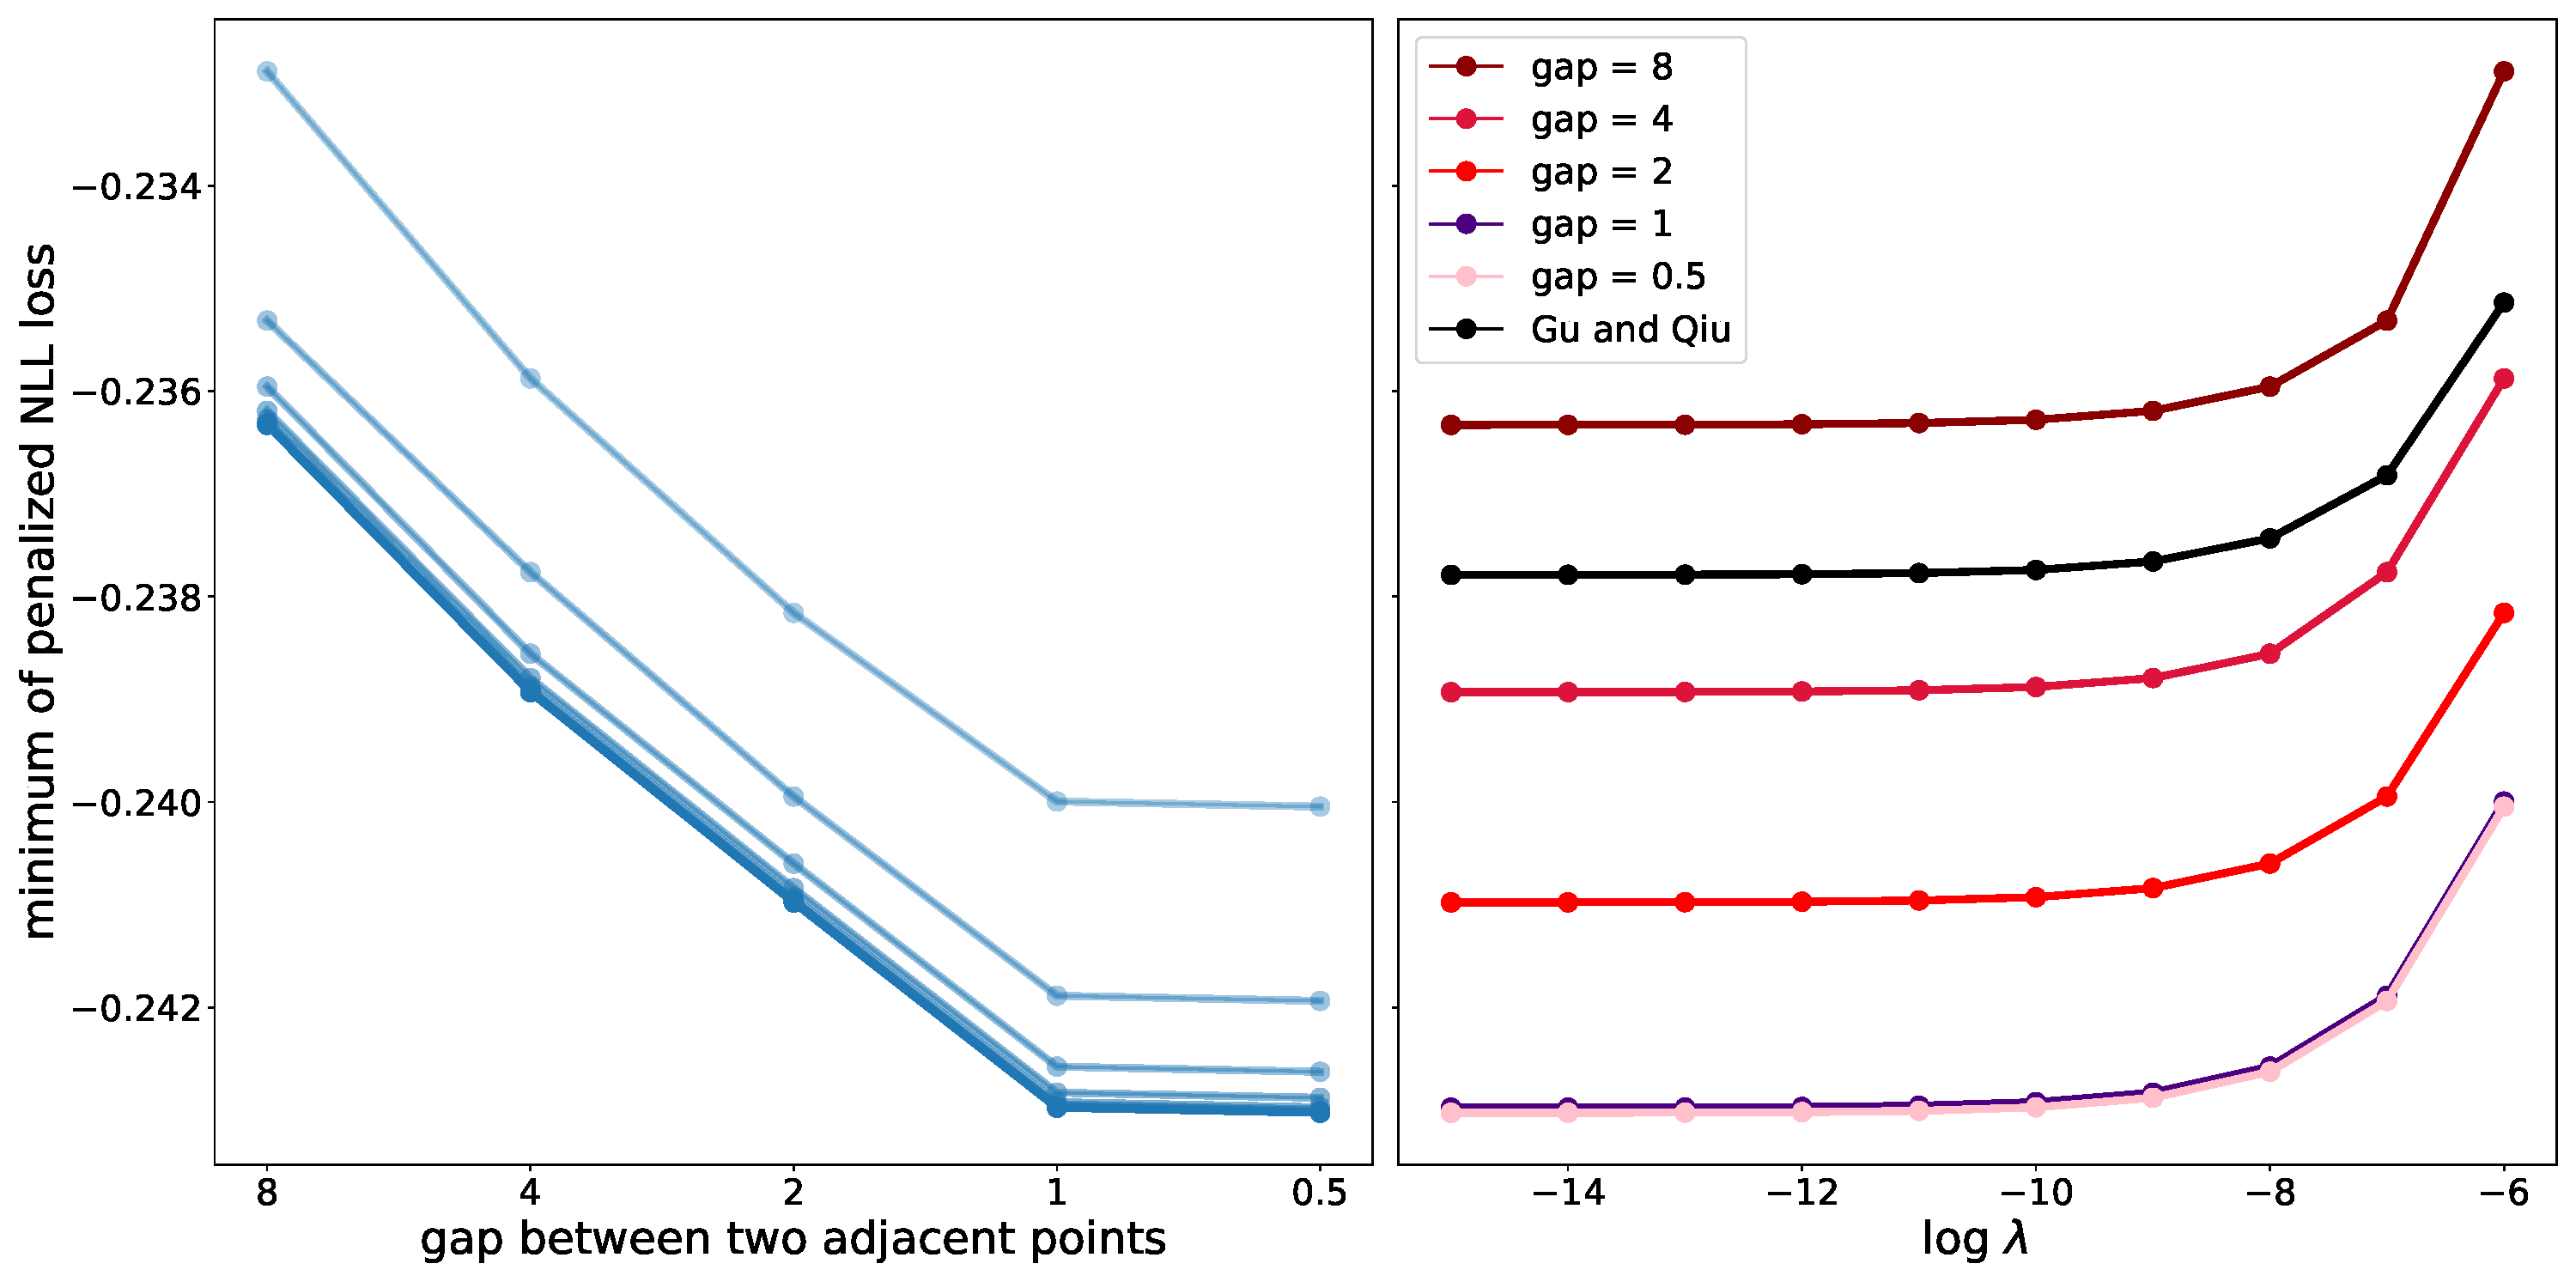
\includegraphics[width=\textwidth]{../plots/choose-best-fin-dim-approx-subspace-bw=5.0.pdf}
	\caption{Left panel: the minimum of $\widetilde{J}_{\NLL, \lambda}$ against the gap between two adjacent points at which kernel functions are centered in different choices of finite-dimensional approximating subspace. Different opacity indicates different values of $\lambda$, and the more opaque line indicates the smaller $\lambda$ value. Right panel: the minimum of $\widetilde{J}_{\NLL, \lambda}$ against different values of $\log \lambda$.}
	\label{fig-choose-fin-dim-approx-subspace}
\end{figure}

The left panel of Figure \ref{fig-choose-fin-dim-approx-subspace} shows the minimum of $\widetilde{J}_{\NLL, \lambda}$ against the gap between two adjacent grid points at which kernel functions are centered in different choices of finite-dimensional approximating subspace. For each value of $\lambda$, we see that, as the gap between two adjacent grid points becomes smaller and smaller, the minimum of $\widetilde{J}_{\NLL, \lambda}$ keeps decreasing. When the difference between two adjacent grid points is 1, if we further insert additional grid points, the further reduction on the minimum of $\widetilde{J}_{\NLL, \lambda}$ becomes negligible. Thus, for this particular \texttt{waiting} data, we use the following subspace as our final choice of the finite-dimensional approximating subspace
\begin{align}\label{eq-final-fin-dim-approx-subspace}
	\widetilde{\calH} := \sets[\Bigg]{f \biggm| f := \sum_{j=1}^{201} \beta_j k \parens{w_j, \,\cdot\,}, \beta_j \in \Real, w_j = j, \text{ for all } j = 1, \cdots, 201}. 
\end{align}

The right panel of Figure \ref{fig-choose-fin-dim-approx-subspace} shows the minimum of $\widetilde{J}_{\NLL, \lambda}$ against different values of $\log \lambda$. Similar to our observations from the left panel, as the gap between two adjacent grid points becomes smaller and smaller, the minimum of $\widetilde{J}_{\NLL, \lambda}$ keeps decreasing for all choices of $\lambda$. Comparing the minimums of $\widetilde{J}_{\NLL, \lambda}$ over the finite-dimensional subspaces with the gap between two adjacent grid points being 1 and 0.5, the difference is very tiny. In addition, the black curve in this panel shows the minimums of $\widetilde{J}_{\NLL, \lambda}$ using the finite-dimensional approximating subspace \eqref{eq-fin-approx-subspace-gu-qiu} that \textcite{Gu1993-na} and \textcite{Gu1993-lf} proposed. It is obvious that our approach yields a smaller minimum of $\widetilde{J}_{\NLL, \lambda}$ than their approach does, implying the superiority of our approach. 

\section{Regularized Score Matching Density Estimators in a Finite-dimensional Approximating Space}\label{section-computation-sm-density-estimator}

We minimize the penalized NLL loss functional over a finite-dimensional approximating space. Since our ultimate goal of this chapter is to compare the regularized SM density estimators and the penalized ML density estimator and understand their similarities and differences, in order to ensure the comparability, we also minimize the (penalized) SM loss functional over the same finite-dimensional subspace of $\calH$. We describe how to achieve this in the current section. 

Throughout this section, we again let 
\begin{align*}
	\widetilde{\calH} :=\sets[\bigg]{f \Bigm| f := \sum_{j=1}^m \beta_j k \parens{w_j, \,\cdot\,}, \beta_j \in \Real \text{ for all } j = 1, 2, \cdots, m} 
\end{align*}
be a finite-dimensional approximating subspace, where $\sets{w_1, \cdots, w_m} \subset \calX$ is a set of specified grid points. We first derive the expression of $\widehat{J}_{\SM} \parens{f}$ with $f \in \widetilde{\calH}$, where $\widehat{J}_{\SM}$ is the SM loss functional given by \eqref{eq-sm-loss-kef} in Chapter \ref{ch2}. 

\begin{proposition}\label{prop-sm-loss-fin-dim-space}
	Let $f = \sum_{j=1}^m w_j k \parens{w_j, \,\cdot\,} \in \widetilde{\calH}$. Then, the SM loss functional can be written as 
	\begin{align*}
		\widetilde{J}_{\SM} \parens{\bbeta} := \frac{1}{2} \bbeta^\top \parens[\bigg]{\frac{1}{n} \bS \bS^\top } \bbeta - \bbeta^\top \bt, 
	\end{align*}
	where $\bbeta := \parens{\beta_1, \cdots, \beta_m}^\top \in \Real^m$, the $\parens{j, \parens{i-1}d + u}$-entry of $\bS \in \Real^{m \times \parens{nd}}$ is $\innerp{k \parens{w_j, \,\cdot\,}}{\partial_u k \parens{X_i, \,\cdot\,}}_{\calH} = \partial_u k \parens{X_i, w_j}$, and the $j$-th entry of $\bt \in \Real^m$ is 
	\begin{align*}
		\innerp{\hat{z}}{k \parens{w_j, \,\cdot\,}} = - \frac{1}{n} \sum_{i=1}^n \sum_{u=1}^d \parens[\big]{\partial_u^2 k \parens{X_i, w_j} + \parens{\partial_u \log \mu} \parens{X_i} \partial_u k \parens{X_i, w_j}}, 
	\end{align*}
	for all $j = 1, \cdots, m$, $i = 1, \cdots, n$ and $u = 1, \cdots, d$. 
\end{proposition}

Proof of Proposition \ref{prop-sm-loss-fin-dim-space} can be found in Section \ref{proof-prop-sm-loss-fin-dim-space}. 

\subsection{Penalized Score Matching Density Estimator}

In order to compute the penalized SM density estimator under the constraint $f \in \widetilde{\calH}$, we minimize the penalized SM loss functional $\widehat{J}_{\SM} \parens{f} + \frac{\rho}{2} \norm{f}_{\calH}^2$ subject to $f \in \widetilde{\calH}$. The following proposition establishes the existence and the uniqueness of this minimizer, and discusses how to compute it. 

\begin{proposition}\label{prop-penalized-sm-fin-dim-space}
	The minimizer of $\widehat{J}_{\SM} \parens{f} + \frac{\rho}{2} \norm{f}_{\calH}^2$ subject to $f \in \widetilde{\calH}$, denoted by $\tilde{f}_{\SM}^{\parens{\rho}}$, exists and is unique, and is given by 
	\begin{align*}
		\tilde{f}_{\SM}^{\parens{\rho}} = \sum_{j=1}^m \beta_{j}^{\parens{\rho}} k \parens{w_j, \,\cdot\,}, 
	\end{align*}
	where $\bbeta_{\SM}^{\parens{\rho}} := \parens{\beta_{1}^{\parens{\rho}}, \beta_{2}^{\parens{\rho}}, \cdots, \beta_{m}^{\parens{\rho}}}^\top \in \Real^m$ satisfies 
	\begin{align*}
		\parens[\bigg]{\frac{1}{n} \bS \bS^\top + \lambda \bK_2} \bbeta_{\SM}^{\parens{\rho}} = \bt, 
	\end{align*}
	where $\bS \in \Real^{m \times \parens{nd}}$ and $\bt \in \Real^m$ are the same as those defined in Proposition \ref{prop-sm-loss-fin-dim-space}, and $\bK_2 \in \Real^{m \times m}$ is the same as the one used in \eqref{eq-nll-opt-problem-beta}. 
\end{proposition}

Proof of Proposition \ref{prop-penalized-sm-fin-dim-space} can be found in Section \ref{proof-prop-penalized-sm-fin-dim-space}. 

\subsection{Early Stopping Score Matching Density Estimator}

We now discuss how to compute the early stopping SM density estimator with $f \in \widetilde{\calH}$. We apply the gradient descent algorithm to minimizing $\widetilde{J}_{\SM}$ over $\Real^m$. The corresponding gradient descent iterates are 
\begin{align}\label{eq-early-stop-sm-fin-dim-space-iterate}
	\bbeta_{\SM}^{\parens{t+1}} = \bbeta_{\SM}^{\parens{t}} - \tau \bracks{ \bM \bbeta_{\SM}^{\parens{t}} - \bt } = \parens{\bI - \tau \bM} \bbeta_{\SM}^{\parens{t}} + \tau \bt, 
\end{align}
where $\bM := \frac{1}{n} \bS \bS^\top$ for notational simplicity, $\bbeta_{\SM}^{\parens{0}} \in \Real^m$ is the starting point of the algorithm, and $\tau > 0$ is the appropriately chosen constant step size. 

The following proposition links $\bbeta_{\SM}^{\parens{t}}$ to $\bbeta_{\SM}^{\parens{0}}$. 

\begin{proposition}\label{prop-early-stop-sm-fin-dim-space}
	For all $t \in \Natural_0$, we have 
	\begin{align}\label{eq-prop-early-stop-sm-fin-dim-space-1}
		\bbeta_{\SM}^{\parens{t+1}} = \parens{\bI - \tau \bM}^{t+1} \bbeta_{\SM}^{\parens{0}} + \tau \sum_{\ell=0}^{t} \parens{\bI - \tau \bM}^{\ell} \bt. 
	\end{align}
	If, in particular, we choose $\bbeta_{\SM}^{\parens{0}} = \boldzero_m$, the $m$-dimensional zero vector, we have 
	\begin{align}\label{eq-prop-early-stop-sm-fin-dim-space-2}
		\bbeta_{\SM}^{\parens{t+1}} = \tau \bQ \widetilde{\bLambda}^{\parens{t+1}} \bQ^\top \bt, \qquad \text{ for all } t \in \Natural_0, 
	\end{align}
	where $\bQ \bLambda \bQ^\top = \bM$ be the eigen-decomposition of $\bM$, $\bQ$ is an orthogonal matrix, $\bLambda$ is a diagonal matrix with all eigenvalues of $\bM$, $\lambda_1 \ge \lambda_2 \cdots \ge \lambda_m$, on the diagonal, and $\widetilde{\bLambda}^{\parens{t+1}}$ is the diagonal matrix with elements on the diagonal being 
	\begin{align*}
		\tilde{\lambda}_j^{\parens{t+1}} = \begin{cases}
			\dfrac{1 - \parens{1 - \tau \lambda_j}^{t+1}}{\tau \lambda_j}, & \, \text{ if } \lambda_j \neq 0, \\ 
			t + 1, & \, \text{ if } \lambda_j = 0, 
		\end{cases}
	\end{align*}
	for all $j = 1, \cdots, m$ and $t \in \Natural_0$. 
\end{proposition}

Proof of Proposition \ref{prop-early-stop-sm-fin-dim-space} can be found in Section \ref{proof-prop-early-stop-sm-fin-dim-space}. 

Using Proposition \ref{prop-early-stop-sm-fin-dim-space}, the $\parens{t+1}$-st gradient descent iterate of $\widehat{J}_{\SM}$ in $\widetilde{\calH}$ is 
\begin{align*}
	\sum_{j=1}^m \beta_{j}^{\parens{t+1}} k \parens{w_j, \,\cdot\,}, 
\end{align*}
where $\beta_{j}^{\parens{t+1}}$ is the $j$-th component of $\bbeta_{\SM}^{\parens{t+1}}$. 


\section{Comparison of Regularized Maximum Likelihood and Score Matching Density Estimators}\label{section-ml-sm-comparison}

With the algorithms of minimizing the penalized NLL loss functional and the (penalized) SM loss functional over a finite-dimensional approximating subspace of $\calH$ shown in the preceding sections, we now use numerical examples to compare the corresponding density estimators and understand their similarities and differences. 

\begin{sidewaysfigure}
	\centering
	
\includegraphics[width=\textwidth]{../plots/waiting-ML-vs-SM-density-estimates-baseden=Gamma-36-2-gridpoint=1-202-1-2.pdf}
	\caption{Penalized ML (first row), penalized SM (second row), and early stopping SM (third row) density estimates of the \texttt{waiting} variable. Histogram of data with the bin width chosen by the Freedman-Diaconis rule is shown in green. The rug plot indicates the location of data and the purple circle indicates the location of the isolated observation 108.}
	\label{fig-sm-ml-compare-with108}
\end{sidewaysfigure}

We again use the \texttt{waiting} variable in the Old Faithful Geyser dataset. Figure \ref{fig-sm-ml-compare-with108} shows the resulting density estimates with different choices of penalty parameters or numbers of iterations. All these density estimates are computed over the finite-dimensional subspace \eqref{eq-final-fin-dim-approx-subspace}. We use the same $\calX$, $\mu$, and $k$ as in Chapter \ref{ch3}. 

From the second and third rows of Figure \ref{fig-sm-ml-compare-with108}, we see that, similar to our findings in Chapter \ref{ch3}, two kinds of regularized SM density estimates are still qualitatively very similar. 

The penalized ML and regularized SM density estimates are qualitatively very similar when there is a large or intermediate amount of regularization. However, they are very different when there is very small regularization (small penalty parameter values or a large number of iterations). Specifically, when a very small regularization is imposed, regularized SM density estimates contains a bump or becomes a spike at the isolated observation, but penalized ML density estimates do not, even when there is no penalty (the case when $\lambda = 0$). 

\begin{sidewaysfigure}
	\centering
	
\includegraphics[width=\textwidth]{../plots/waiting-ML-vs-SM-density-estimates-baseden=Gamma-36-2-gridpoint=1-202-1-no108-2.pdf}
	\caption{Penalized ML (first row), penalized SM (second row), and early stopping SM (third row) density estimates of the \texttt{waiting} variable with the isolated observation 108 removed. Histogram of data with the bin width chosen by the Freedman-Diaconis rule is shown in green. The rug plot indicates the location of data.}
	\label{fig-sm-ml-compare-no108}
\end{sidewaysfigure}

If we remove this isolated observation 108, as is shown in Figure \ref{fig-sm-ml-compare-no108}, regularized SM density estimates do not contain a spike when the regularization is small. 

Based on these numerical examples, we conclude that the regularized SM density estimators are very sensitive to the presence of an isolated observation, especially when there is a small amount of regularization. Additional numerical examples confirm this. 


\section{Discussion on the Presence of a Spike in Score Matching Density Estimates}\label{section-sm-explanation}

We now attempt to explain why the regularized SM density estimates put a spike at the isolated observation when regularization is very small. With $d = 1$, we can write the SM loss functional as 
\begin{align*}% \label{eq-sm-loss-explain}
	\widehat{L}_{\SM} \parens{q_f} = & \, \underbrace{\frac{1}{n} \sum_{i \neq i^*} \parens[\bigg]{\frac{1}{2} \parens[\big]{ \parens{\log q_f}' \parens{X_i}}^2 + \parens{\log q_f}'' \parens{X_i}}}_{=: \parens{\mathrm{I}}} + \nonumber \\ 
	& \qquad \qquad \underbrace{\frac{1}{n} \parens[\bigg]{\frac{1}{2} \parens[\big]{ \parens{\log q_f}' \parens{X_{i^*}}}^2 + \parens{\log q_f}'' \parens{X_{i^*}}}}_{=: \parens{\mathrm{II}}}, 
\end{align*}
where $X_{i^*}$ denotes the isolated observation. 

Recall that the penalized SM density estimator is obtained by minimizing $\widehat{L}_{\SM} \parens{q_f} + \frac{\rho}{2} \norm{f}_{\calH}^2$. When $\rho$ is tiny, we are effectively minimizing the $\widehat{L}_{\SM}$ part. Notice $\log q_f$ is a linear combination of $\log \mu$ and Gaussian kernel functions centered at a set of grid points or the first two derivatives of Gaussian kernels centered at data points (depending on which basis functions we use), and these Gaussian kernel functions and derivatives of Gaussian kernel functions are local basis functions. Also, note that a spike is essentially a local maximum. Consequently, putting a spike in $\log q_f$ at $X_{i^*}$ has the effects of forcing $\parens{\parens{\log q_f}' \parens{X_{i^*}}}^2 \approx 0$ and reducing the value of $\parens{\log q_f}'' \parens{X_{i^*}}$ and, hence, that of (II) a lot, without affecting $\parens{\mathrm{I}}$ much. Thus, putting a spike at $X_{i^*}$ can reduce the value of $\widehat{L}_{\SM}$, coinciding with the goal of minimizing $\widehat{L}_{\SM}$. 

A similar explanation holds for the early stopping SM density estimator. As we keep running the gradient descent algorithm, we are searching for a $q_f \in \calQ_{\ker}$ that can reduce the value of $\widehat{L}_{\SM}$ as much as possible. With an isolated observation $X_{i^*}$ being present and local basis functions being used, putting a spike at $X_{i^*}$ can achieve this goal. 

\newpage

\section{Proofs}\label{section-proof}

\subsection{Proof of Proposition \ref{prop-nll-sol-exist-unique}}\label{proof-prop-nll-sol-exist-unique}

\begin{proof}[Proof of Proposition \ref{prop-nll-sol-exist-unique}]
	First, by \ref{assumption-2-2-bdd-kernel} in Chapter \ref{ch2}, we know $\calF = \calH$ so that minimizing \eqref{eq-pen-nll-loss} over $\calH$ is an unconstrained minimization problem. 
	
	By \ref{assumption-2-3-no-const-fun} and Theorem \ref{prop-convexity-A} in Chapter \ref{ch2}, we know $A$ is strictly convex. In addition, since $\frac{1}{n} \sum_{i=1}^n f \parens{X_i} = \frac{1}{n} \sum_{i=1}^n \innerp{f}{k \parens{X_i, \,\cdot\,}}$ is convex in $f$, we conclude $\widehat{J}_{\NLL}$ is convex. In addition, note that the functional $f \mapsto \frac{\lambda}{2} \norm{f}_{\calH}^2$ is strongly convex with constant $\lambda > 0$. It follows that the objective functional in \eqref{eq-pen-nll-loss} is strongly convex with constant $\lambda > 0$ \parencite[Proposition 10.8 in][]{Bauschke2017-he}. Finally, Corollary 11.17 in \textcite{Bauschke2017-he} implies \eqref{eq-pen-nll-loss} has exactly one minimizer in $\calH$. 
\end{proof}


\subsection{Details about Example \ref{example-representer-theorem-fails}}\label{proof-example-representer-theorem-fails}

	We provide details about Example \ref{example-representer-theorem-fails} here, and will follow three steps: 
	\begin{enumerate}
		\item[] Step 1. Identify the RKHS $\calH$ associated with the choice of $k$ and the corresponding natural parameter space $\calF$; 
		\item[] Step 2. Identify $\mathrm{Span} \sets{k \parens{X_1, \,\cdot\,}}$ and $\mathrm{Span} \sets{k \parens{X_1, \,\cdot\,}} \cap \calF$; 
		\item[] Step 3. Explcitly compute the minimizer of \eqref{eq-example-nll-representer-theorem-fails-1} over $\calF$ and show this minimizer does not reside in $\mathrm{Span} \sets{k \parens{X_1, \,\cdot\,}} \cap \calF$. 
	\end{enumerate}
	
	\underline{Step 1.} Letting $x = \parens{x_1, x_2}^\top \in \Real^2$ and $y = \parens{y_1, y_2}^\top \in \Real^2$ be arbitrary, we have 
	\begin{align*}
		k \parens{x, y} = \parens{x^\top y}^2 
		%= & \, \parens{x_1 y_1 + x_2 y_2}^2 \\ 
		= x_1^2 y_1^2 + 2 x_1 x_2 y_1 y_2 + x_2^2 y_2^2 
		= \innerp{\Phi \parens{x}}{\Phi \parens{y}}, \qquad \text{ for all } x, y \in \Real, 
%		= & \, \begin{pmatrix}
%			x_1^2 \\ \sqrt{2} x_1 x_2 \\ x_2^2
%		\end{pmatrix}^\top 
%		\begin{pmatrix}
%			y_1^2 \\ \sqrt{2} y_1 y_2 \\ y_2^2
%		\end{pmatrix} \\ 
%		= & \, \innerp[\Bigg]{\begin{pmatrix}
%			x_1^2 \\ \sqrt{2} x_1 x_2 \\ x_2^2
%		\end{pmatrix}}{\begin{pmatrix}
%			y_1^2 \\ \sqrt{2} y_1 y_2 \\ y_2^2
%		\end{pmatrix}}. 
	\end{align*}
	where $\Phi: \Real^2 \to \Real^3$ denotes the feature map of $k$ and is given by 
	\begin{align*}
		\Phi \parens{x} = \parens[\Big]{x_1^2, \sqrt{2} x_1 x_2, x_2^2}^{\top}, %\qquad \text{ for all } x = \parens{x_1, x_2} \in \Real^2, 
	\end{align*}
	and the inner product $\innerp{\,\cdot\,}{\,\cdot\,}$ is the dot product in $\Real^3$. Then, the resulting $\calH$ contains all functions mapping from $\Real^2$ to $\Real$ of the form 
	\begin{align*}
		f \parens{x} 
		%= f^\top \Phi \parens{x} = \innerp{f}{\Phi \parens{x}} 
		= w_1 x_1^2 + \sqrt{2} w_2 x_1 x_2 + w_3 x_2^2, \qquad \text{ for all } x = \parens{x_1, x_2}^\top \in \Real^2, 
	\end{align*}
	for some $w_1, w_2, w_3 \in \Real$ with the RKHS norm of $f$ being $\norm{f}_{\calH} = \sqrt{w_1^2 + w_2^2 + w_3^2}$ \parencite[Theorem 4.21 in][]{Steinwart2008-tn}. 
	
	We now derive the natural parameter space $\calF$. Let $f \parens{x} = w_1 x_1^2 + \sqrt{2} w_2 x_1 x_2 + w_3 x_2^2$ for some $w_1, w_2, w_3 \in \Real$ and all $x = \parens{x_1, x_2}^\top \in \Real^2$. By simple algebra, we have 
	\begin{align*}
		e^{A \parens{f}} = & \, \int \int_{\Real^2} \frac{1}{2\pi} \exp \parens[\bigg]{- \frac{\norm{x}_2^2}{2}} \exp \parens[\big]{f \parens{x}} \diff x_1 \diff x_2 
		%  = & \, \int \int_{\Real^2} \frac{1}{2\pi} \exp \parens[\bigg]{- \frac{x_1^2 + x_2^2}{2} + w_1 x_1^2 + \sqrt{2} w_2 x_1 x_2 + w_3 x_2^2} \diff x_1 \diff x_2 \\ 
		 % = & \, \int \int_{\Real^2} \frac{1}{2\pi} \exp \parens[\bigg]{- \frac{1}{2} \parens[\big]{x_1^2 + x_2^2 - 2 w_1 x_1^2 - 2 \sqrt{2} w_2 x_1 x_2 - 2 w_3 x_2^2}} \diff x_1 \diff x_2 \\ 
		 % = & \, \int \int_{\Real^2} \frac{1}{2\pi} \exp \parens[\bigg]{- \frac{1}{2} \parens[\big]{\parens{1 - 2 w_1} x_1^2 - 2 \sqrt{2} w_2 x_1 x_2 + \parens{1 - 2 w_3} x_2^2}} \diff x_1 \diff x_2 \\ 
		 % = & \, \int \int_{\Real^2} \frac{1}{2\pi} \exp \parens[\bigg]{- \frac{1}{2} x^\top W^{-1} x} \diff x_1 \diff x_2 \\ 
		 % = & \, \int \int_{\Real^2} \frac{\abs{W}^{1/2}}{2\pi \abs{W}^{1/2}} \exp \parens[\bigg]{- \frac{1}{2} x^\top W^{-1} x} \diff x_1 \diff x_2 \\ 
		 = \abs{W}^{1/2}, 
	\end{align*}
	where $\abs{W}$ denotes the determinant of the matrix $W$, 
	\begin{align*}
		W^{-1} = \begin{pmatrix}
			1 - 2w_1 & -\sqrt{2} w_2 \\ -\sqrt{2} w_2 & 1 - 2w_3
		\end{pmatrix}, 
	\end{align*}
	and we assume $\parens{1 - 2 w_1} \parens{1 - 2 w_3} - 2w_2^2 > 0$. Then, 
	\begin{align*}
		A \parens{f} = \log \parens[\big]{\abs{W}^{1/2}} = -\frac{1}{2} \log \parens[\big]{\parens{1 - 2w_1} \parens{1 - 2w_3} - 2 w_2^2}. 
	\end{align*}
	Note that $A \parens{f} < \infty$ if and only if $W$ is positive definite if and only if $1 - 2w_1 > 0$ and $1 - 2 w_3 > 0$ and $\parens{1 - 2w_1} \parens{1 - 2w_3} - 2 w_2^2 > 0$ if and only if $w_1 < \frac{1}{2}$ and $w_3 < \frac{1}{2}$ and $\parens{1 - 2w_1} \parens{1 - 2w_3} - 2 w_2^2 > 0$. 
	
	As the conclusion of Step 1, we have 
	\begin{align}
		\calH = & \, \bigg\{f: \Real^2 \to \Real \Bigm| f \parens{x} := w_1 x_1^2 + \sqrt{2} w_2 x_1 x_2 + w_3 x_2^2 \text{ for all } x = \parens{x_1, x_2}^\top \in \Real^2, \nonumber \\ 
		& \quad \quad \qquad \qquad \qquad w_1, w_2, w_3 \in \Real \bigg\}, \label{eq-example-nll-representer-theorem-fails-rkhs} \\ 
		\calF = & \, \bigg\{f: \Real^2 \to \Real \Bigm| f \parens{x} = w_1 x_1^2 + \sqrt{2} w_2 x_1 x_2 + w_3 x_2^2 \text{ for all } x = \parens{x_1, x_2}^\top \in \Real^2, \nonumber \\ 
		& \quad \qquad \qquad \qquad \quad w_1 < \frac{1}{2}, w_3 < \frac{1}{2}, \parens{1 - 2w_1} \parens{1 - 2w_3} - 2 w_2^2 > 0, w_1, w_2, w_3 \in \Real \bigg\}. \label{eq-example-nll-representer-theorem-fails-F}
	\end{align}
	
	\underline{Step 2.} With $X_1 = \parens{a, 0}^\top$, it is easy to see $\mathrm{Span} \sets{k \parens{X_1, \,\cdot\,}}$ contains all functions of the form 
	\begin{align*}
		f \parens{x} = \gamma k \parens{X_1, x} = \gamma \parens{X_1^\top x}^2 = \gamma a^2 x_1^2, \quad \text{ for all } x := \parens{x_1, x_2}^\top \in \Real^2 \text{ and } \gamma \in \Real. 
	\end{align*}
	Then, we can characterize $\mathrm{Span} \sets{k \parens{X_1, \,\cdot\,}} \cap \calF$ as 
	\begin{align*}
		\mathrm{Span} \sets{k \parens{X_1, \,\cdot\,}} \cap \calF = \bigg\{f: \Real^2 \to \Real \Bigm| f \parens{x} = \gamma a^2 x_1^2 \text{ for all } x = \parens{x_1, x_2}^\top \in \Real^2, \gamma a^2 < \frac{1}{2} \bigg\}. 
	\end{align*}
	
	\underline{Step 3.} Let $f \in \calF$ be 
	\begin{align*}
		f \parens{x} = w_1 x_1^2 + \sqrt{2} w_2 x_1 x_2 + w_3 x_2^2, \qquad \text{ for all } x = \parens{x_1, x_2}^\top \in \Real^2, 
	\end{align*}
	where $w_1, w_2, w_3 \in \Real$ satisfy the constraints in \eqref{eq-example-nll-representer-theorem-fails-F}. Then, with $\lambda > 0$, $\widehat{J}_{\NLL} \parens{f} + \frac{\lambda}{2} \norm{f}_{\calH}^2$ becomes  
	\begin{align*}
		\widetilde{J}_{\lambda} \parens{w_1, w_2, w_3} := & \, - \frac{1}{2} \log \parens[\big]{\parens{1 - 2w_1} \parens{1 - 2w_3} - 2 w_2^2} - w_1 a^2 + \frac{\lambda}{2} \parens{w_1^2 + w_2^2 + w_3^2}. 
	\end{align*}
	By calculus, we have 
	\begin{align*}
		\nabla \widetilde{J}_{\lambda} \parens{w_1, w_2, w_3} = & \, \begin{pmatrix}
			\frac{1 - 2w_3}{\parens{1-2w_1} \parens{1-2w_3} - 2w_2^2} - a^2 + \lambda w_1 \\ 
			\frac{2w_2}{\parens{1-2w_1} \parens{1-2w_3} - 2w_2^2} + \lambda w_2 \\
			\frac{1 - 2w_1}{\parens{1-2w_1} \parens{1-2w_3} - 2w_2^2} + \lambda w_3
		\end{pmatrix}.  
	\end{align*}
	Any stationary points, denoted by $\parens{w_1^*, w_2^*, w_3^*}$, must satisfy $\nabla \widetilde{J}_{\lambda} \parens{w_1^*, w_2^*, w_3^*} = 0$, from which we obtain the following system of equations 
	\begin{align*}
		\begin{cases}
			\parens{1 - 2 w_3^*} + \parens{\lambda w_1^* - a^2} \parens[\big]{\parens{1 - 2w_1^*} \parens{1 - 2w_3^*} - 2{w_2^*}^2} & = 0, \\ 
			2 w_2^* + \lambda w_2^* \parens[\big]{\parens{1 - 2 w_1^*} \parens{1 - 2 w_3^*} - 2 {w_2^*}^2} & = 0, \\ 
			\parens{1 - 2 w_1^*} + \lambda w_3^* \parens[\big]{\parens{1 - 2w_1^*} \parens{1 - 2w_3^*} - 2{w_2^*}^2} & = 0. 
		\end{cases}	
	\end{align*}
	Solving the preceding system for $\parens{w_1^*, w_2^*, w_3^*}$ yields the following solutions: 
	\begin{align}\label{eq-example-all-sol}
		\parens[\bigg]{\frac{1}{2}, \, 0, \, \frac{1}{2}}, \quad \parens[\big]{b_1^*, \, 0, \, c_1^*}, \quad \parens[\big]{b_1^*, \, 0, \, c_2^*}, \quad \parens[\big]{b_2^*, \, 0, \, c_1^*}, \quad \parens[\big]{b_2^*, \, 0, \, c_2^*}, 
	\end{align}
	where 
	\begin{align*}
		& \, b_1^* := \frac{\parens{\lambda + 2 a^2} + \sqrt{\parens{\lambda - 2 a^2}^2 + 8 \lambda}}{4 \lambda}, 
		&& \, b_2^* := \frac{- \parens{\lambda + 2 a^2} + \sqrt{\parens{\lambda - 2 a^2}^2 + 8 \lambda}}{-4 \lambda}, \\ 
		& \, c_1^* := \frac{\lambda + \sqrt{\lambda^2 + 8 \lambda}}{4 \lambda}, 
		&& \, c_2^* := \frac{\lambda - \sqrt{\lambda^2 + 8 \lambda}}{4 \lambda}. 
	\end{align*}
	We next check whether the corresponding functions belong to $\calF$ or not. 
	
	First, notice that the pair of $\parens{w_1^*, w_2^*, w_3^*} = \parens{\frac{1}{2}, 0, \frac{1}{2}}$ leads to the function $f \parens{x} = \frac{1}{2} \parens{x_1^2 + x_2^2}$, which does \textit{not} belong to $\calF$ since $w_1^* = \frac{1}{2}$ and $w_3^* = \frac{1}{2}$. We discard it. 
	
	In addition, since $\lambda > 0$, we have 
	\begin{align*}
		b_1^* = \frac{\parens{\lambda + 2 a^2} + \sqrt{\parens{\lambda - 2 a^2}^2 + 8 \lambda}}{4 \lambda} > \frac{\parens{\lambda + 2 a^2} + \abs{\lambda - 2 a^2}}{4 \lambda}. 
	\end{align*}
	Consider the following two cases: 
	\begin{enumerate}
		\item[(i)] If $2 a^2 - \lambda \ge 0$, that is, $a^2/\lambda \ge \frac{1}{2}$, we have $b_1^* > \frac{\lambda + 2 a^2 + 2 a^2 - \lambda}{4 \lambda} = \frac{a^2}{\lambda} \ge \frac{1}{2}$; 

		\item[(ii)] If $2 a^2 - \lambda < 0$, we have $b_1^* > \frac{\lambda + 2 a^2 + \lambda - 2 a^2}{4 \lambda} = \frac{2\lambda}{4\lambda} \ge \frac{1}{2}$. 
	\end{enumerate}
	In both cases, we have $b_1^* > \frac{1}{2}$, and any function $f$ with $w_1^* = b_1^*$ cannot belong to $\calF$. 
	
	Next, we show $b_2^* < \frac{1}{2}$, which is equivalent to showing $1 - 2b_2^* > 0$. Since 
	\begin{align*}
		1 - 2b_2^* = & \, 1 - \frac{- \parens{\lambda + 2 a^2} + \sqrt{\parens{\lambda - 2 a^2}^2 + 8 \lambda}}{-2 \lambda} \\ 
		= & \, 1 + \frac{\sqrt{\parens{\lambda - 2 a^2}^2 + 8 \lambda} - \parens{\lambda + 2 a^2}}{2 \lambda} \\ 
		> & \, 1 + \frac{\abs{\lambda - 2 a^2} - \parens{\lambda + 2 a^2}}{2 \lambda}. 
	\end{align*}
	Again, we consider the following two cases: 
	\begin{enumerate}
		\item[(i)] If $2 a^2 - \lambda \ge 0$, we have $1 - 2 b_2^* > 1 + \frac{2 a^2 - \lambda - \lambda - 2a^2}{2 \lambda} = 1 + \frac{- 2\lambda }{2 \lambda} = 0$; 
		\item[(ii)] If $2 a^2 - \lambda < 0$, that is, $0 \le a^2 / \lambda < \frac{1}{2}$, we have $1 - 2b_2^* > 1 + \frac{\lambda - 2 a^2 - \lambda - 2 a^2}{2 \lambda} = 1 - \frac{2 a^2}{\lambda} > 0$. 
	\end{enumerate}
	
	As for $c_1^*$ and $c_2^*$, since $\lambda > 0$, we have 
	\begin{align*}
		c_1^* = & \, \frac{\lambda + \sqrt{\lambda^2 + 8 \lambda}}{4 \lambda} > \frac{\lambda + \sqrt{\lambda^2}}{4 \lambda} = \frac{1}{2}, \\ 
		c_2^* = & \, \frac{\lambda - \sqrt{\lambda^2 + 8 \lambda}}{4 \lambda} < \frac{\lambda}{4 \lambda} = \frac{1}{4} < \frac{1}{2}. 
	\end{align*}
	That is, any function $f$ with $w_3^* = c_1^*$ cannot belong to $\calF$. 
	
	As a conclusion, the only solution in \eqref{eq-example-all-sol} such that the resulting $f$ belongs to $\calF$ is $\parens{w_1^*, w_2^*, w_3^*} = \parens{b_2^*, 0, c_2^*}$. 
	
	In addition, it is easy to see that the Hessian matrix of $\widetilde{J}_{\lambda}$ at $\parens{w_1^*, w_2^*, w_3^*} = \parens{b_2^*, 0, c_2^*}$ is 
	\begin{align*}
		\begin{pmatrix}
			\frac{2 \parens{1 - c_2^*}^2}{\parens{1 - 2b_2^*}^2 \parens{1 - 2c_2^*}^2} + \lambda & 0 & 0 \\ 
			0 & \frac{2 \parens{1 - b_2^*} \parens{1 - c_2^*}}{\parens{1 - 2b_2^*}^2 \parens{1 - 2c_2^*}^2} + \lambda & 0 \\ 
			0 & 0 & \frac{2 \parens{1 - b_2^*}^2}{\parens{1 - 2b_2^*}^2 \parens{1 - 2c_2^*}^2} + \lambda
		\end{pmatrix}, 
	\end{align*}
	which is positive definite. We conclude that $\widetilde{J}_{\lambda}$ achieves the minimum at $\parens{w_1^*, w_2^*, w_3^*} = \parens{b_2^*, 0, c_2^*}$, and the corresponding function, $f^* := \argmin_{f \in \calF} \braces[\big]{\widehat{J}_{\NLL} \parens{f} + \frac{\lambda}{2} \norm{f}_{\calH}^2}$, is 
	\begin{align*}% \label{ex.optf}
		f^* \parens{x} = b_2^* x_1^2 + c_2^* x_2^2, \qquad \text{ for all } x = \parens{x_1, x_2}^\top \in \Real^2. 
	\end{align*}
	Since $c_2^* \neq 0$ for all $\lambda > 0$, $f^*$ does \emph{not} belong to $\mathrm{Span} \sets{k \parens{X_1, \,\cdot\,}} \cap \calF$. \hfill \qedsymbol


\subsection{Proof of Proposition \ref{prop-sm-loss-fin-dim-space}}\label{proof-prop-sm-loss-fin-dim-space}

\begin{proof}[Proof of Proposition \ref{prop-sm-loss-fin-dim-space}]
	Since $f \in \widetilde{\calH}$ takes on the form $f = \sum_{j=1}^m \beta_j k \parens{w_j, \,\cdot\,}$ for $\beta_1, \cdots, \beta_m \in \Real$, we first have 
	\begin{align*}
		& \, \innerp{f}{\parens{\partial_u k \parens{X_i, \,\cdot\,} \otimes \partial_u k \parens{X_i, \,\cdot\,}} f}_{\calH} \nonumber \\ 
		= & \, \innerp[\bigg]{\sum_{\ell=1}^m \beta_{\ell} k \parens{w_\ell, \,\cdot\,}}{\parens{\partial_u k \parens{X_i, \,\cdot\,} \otimes \partial_u k \parens{X_i, \,\cdot\,}} \parens[\bigg]{\sum_{j=1}^m \beta_j k \parens{w_j, \cdot}}}_{\calH} \nonumber \\ 
		% = & \, \sum_{\ell=1}^m \sum_{j=1}^m \alpha_{\ell} \alpha_j \innerp[\big]{k \parens{w_\ell, \cdot}}{\parens{\partial_u k \parens{X_i, \cdot} \otimes \partial_u k \parens{X_i, \cdot}} k \parens{w_j, \cdot}}_{\calH} \nonumber \\ 
		= & \, \sum_{\ell=1}^m \sum_{j=1}^m \beta_{\ell} \beta_j \innerp{\partial_u k \parens{X_i, \,\cdot\,}}{k \parens{w_\ell, \,\cdot\,}}_{\calH} \innerp{\partial_u k \parens{X_i, \,\cdot\,}}{k \parens{w_j, \,\cdot\,}}_{\calH} \nonumber \\ 
		= & \, \sum_{\ell=1}^m \sum_{j=1}^m \beta_{\ell} \beta_j \partial_u k \parens{X_i, w_\ell} \partial_u k \parens{X_i, w_j}, 
	\end{align*}
	where the last equality is due to the reproducing property of the partial derivative of $k$ (see Proposition \ref{prop-reproducing-derivative} in Appendix \ref{app1}). Then, since $\widehat{C} = \frac{1}{n} \sum_{i=1}^n \sum_{u=1}^d \partial_u k \parens{X_i, \,\cdot\,} \otimes \partial_u k \parens{X_i, \,\cdot\,}$, by the linearity of the inner product, we have 
	\begin{align*}
		\innerp{f}{\widehat{C} f}_{\calH} = & \, \frac{1}{n} \sum_{i=1}^n \sum_{u=1}^d \innerp[\big]{f}{\parens{\partial_u k \parens{X_i, \cdot} \otimes \partial_u k \parens{X_i, \cdot}} f}_{\calH} \nonumber \\ 
		= & \, \frac{1}{n} \sum_{i=1}^n \sum_{u=1}^d \sum_{\ell=1}^m \sum_{j=1}^m \beta_{\ell} \beta_j \partial_u k \parens{X_i, w_\ell} \partial_u k \parens{X_i, w_j} \\ 
		% = & \, \bbeta^\top \parens[\bigg]{\frac{1}{n} \sum_{i=1}^n \sum_{u=1}^d \bg_{\parens{i - 1}d + u} \bg_{\parens{i - 1}d + u}^\top } \bbeta \nonumber \\ 
		= & \, \bbeta^\top \parens[\bigg]{\frac{1}{n} \bS \bS^\top } \bbeta. 
	\end{align*}
%	where 
%	\begin{align}
%		\bg_{\parens{i-1}d+u} = \begin{pmatrix}
%			\partial_u k \parens{X_i, w_1}, 
%			\partial_u k \parens{X_i, w_2}, 
%			\cdots, 
%			\partial_u k \parens{X_i, w_m}
%		\end{pmatrix}^\top \in \Real^m, 
%	\end{align}
%	for all $i = 1, \cdots, n$ and $u = 1, \cdots, d$, and 
%	\begin{align}
%		\bG = \begin{pmatrix}
%			\bg_1 \, \vdots \, \bg_2 \, \vdots \, \cdots \, \vdots \, \bg_{nd}
%		\end{pmatrix} \in \Real^{m \times \parens{nd}}. 
%	\end{align}

	As for $\innerp{f}{\hat{z}}_{\calH}$, we have the following 
	\begin{align*}
		\innerp{f}{\hat{z}}_{\calH} = & \, \innerp[\bigg]{\sum_{j=1}^m \beta_j k \parens{w_j, \,\cdot\,}}{- \frac{1}{n} \sum_{i=1}^n \sum_{u=1}^d \parens[\big]{\partial_u^2 k \parens{X_i, \,\cdot\,} + \parens{\partial_u \log \mu} \parens{X_i} \partial_u k \parens{X_i, \,\cdot\,}}}_{\calH} \\ 
		= & \, \sum_{j=1}^m \beta_j \parens[\bigg]{- \frac{1}{n} \sum_{i=1}^n \sum_{u=1}^d \parens[\big]{\partial_u^2 k \parens{X_i, w_j} + \parens{\partial_u \log \mu} \parens{X_i} \partial_u k \parens{X_i, w_j}} } \\ 
		= & \, \bbeta^\top \bt, 
	\end{align*}
	where we use the reproducing property of the partial derivative of $k$ in the second equality. The desired result follows by combining all pieces above together. 
\end{proof}


\subsection{Proof of Proposition \ref{prop-penalized-sm-fin-dim-space}}\label{proof-prop-penalized-sm-fin-dim-space}

\begin{proof}[Proof of Proposition \ref{prop-penalized-sm-fin-dim-space}]
	Recall from Chapters \ref{ch2} and \ref{ch3} that the operator $\widehat{C}: \calH \to \calH$ is positive semidefinite, $\widehat{J}_{\SM}$ is convex over $\calH$. In addition, note that the functional $f \mapsto \frac{\rho}{2} \norm{f}_{\calH}^2$ is strongly convex with constant $\rho$. We conclude that the penalized SM loss functional $f \mapsto \widehat{J}_{\SM} \parens{f} + \frac{\rho}{2} \norm{f}_{\calH}^2$ is strongly convex with parameter $\lambda > 0$, and that it has exactly one minimizer \parencite[Corollary 11.17 in][]{Bauschke2017-he}. 
	
	With $f = \sum_{j=1}^m \beta_j k \parens{w_j, \,\cdot\,} \in \widetilde{\calH}$, we have $\frac{\rho}{2} \norm{f}_{\calH}^2 = \frac{\rho}{2} \bbeta^\top \bK_2 \bbeta$. Thus, together with Proposition \ref{prop-sm-loss-fin-dim-space}, we can write the functional $\widehat{J}_{\SM} \parens{f} + \frac{\rho}{2} \norm{f}_{\calH}^2$ with $f \in \widetilde{\calH}$ as 
	\begin{align*}
		\widetilde{J}_{\SM, \rho} \parens{\bbeta} := \frac{1}{2} \bbeta^\top \parens[\bigg]{\frac{1}{n} \bS \bS^\top} \bbeta - \bbeta^\top \bt + \frac{\rho}{2} \bbeta^\top \bK_2 \bbeta. 
	\end{align*}
	Then, $\bbeta_{\SM}^{\parens{\rho}} := \argmin_{\bbeta \in \Real^m} \widetilde{J}_{\SM, \rho} \parens{\bbeta}$ must satisfy the first-order optimality condition 
	\begin{align*}
		\parens[\bigg]{\frac{1}{n} \bS \bS^\top + \rho \bK_2} \bbeta_{\SM}^{\parens{\rho}} = \bt. 
	\end{align*}
	As a consequence, $\argmin_{f \in \widetilde{\calH}} \sets[\big]{\widehat{J}_{\SM} \parens{f} + \frac{\rho}{2} \norm{f}_{\calH}^2}$ is $\sum_{j=1}^m \beta_j^{\parens{\rho}} k \parens{w_j, \,\cdot\,}$, where $\beta_j^{\parens{\rho}}$ is the $j$-th element of $\bbeta_{\SM}^{\parens{\rho}}$. 
\end{proof}


\subsection{Proof of Proposition \ref{prop-early-stop-sm-fin-dim-space}}\label{proof-prop-early-stop-sm-fin-dim-space}

\begin{proof}[Proof of Proposition \ref{prop-early-stop-sm-fin-dim-space}]
	We first prove \eqref{eq-prop-early-stop-sm-fin-dim-space-1} by induction. When $t = 0$, from \eqref{eq-early-stop-sm-fin-dim-space-iterate}, we have 
	\begin{align}\label{eq-prop-early-stop-sm-fin-dim-space-3}
		\bbeta_{\SM}^{\parens{1}} = \parens{\bI - \tau \bM} \bbeta_{\SM}^{\parens{0}} + \tau \bt. 
	\end{align}
	From \eqref{eq-prop-early-stop-sm-fin-dim-space-1}, we plug in $t=0$ and obtain 
	\begin{align*}
		\bbeta_{\SM}^{\parens{1}} = & \, \parens{\bI - \tau \bM} \bbeta_{\SM}^{\parens{0}} + \tau \sum_{\ell=0}^{0} \parens{\bI - \tau \bM}^i \bt 
		= \parens{\bI - \tau \bM} \bbeta_{\SM}^{\parens{0}} + \tau \bt, 
	\end{align*}
	which is identical to \eqref{eq-prop-early-stop-sm-fin-dim-space-3}. 
	
	Now, supposing \eqref{eq-prop-early-stop-sm-fin-dim-space-1} holds for $t = s$, we are going to show it also holds for $t = s+1$. Note the following 
	\begin{align}
		\bbeta_{\SM}^{\parens{s+1}} = & \, \parens{\bI - \tau \bM} \bbeta_{\SM}^{\parens{s}} + \tau \bt \nonumber \\ 
		= & \, \parens{\bI - \tau \bM} \bracks[\bigg]{\parens{\bI - \tau \bM}^s \bbeta_{\SM}^{\parens{0}} + \tau \sum_{\ell=0}^{s-1} \parens{\bI - \tau \bM}^{\ell} \bt } + \tau \bt \nonumber \\ 
		= & \, \parens{\bI - \tau \bM}^{s+1} \bbeta_{\SM}^{\parens{0}} + \tau \sum_{\ell=0}^{s-1} \parens{\bI - \tau \bM}^{\ell+1} \bt + \tau \bt \nonumber \\ 
		= & \, \parens{\bI - \tau \bM}^{s+1} \bbeta_{\SM}^{\parens{0}} + \tau \sum_{\ell=1}^{s} \parens{\bI - \tau \bM}^{\ell} \bt + \tau \bt \nonumber \\ 
		= & \, \parens{\bI - \tau \bM}^{s+1} \bbeta_{\SM}^{\parens{0}} + \tau \sum_{\ell=0}^{s} \parens{\bI - \tau \bM}^{\ell} \bt, \nonumber
	\end{align}
	which is the desired result. 
	
	We now prove \eqref{eq-prop-early-stop-sm-fin-dim-space-2}. With $\bbeta_{\SM}^{\parens{0}} = \boldzero_m$, we can simplify \eqref{eq-prop-early-stop-sm-fin-dim-space-1} to 
\begin{align*}% \label{eq-prop}
	\bbeta_{\SM}^{\parens{t+1}} = \tau \sum_{\ell=0}^{t} \parens{\bI - \tau \bM}^{\ell} \bt, \qquad \text{ for all } t \in \Natural_0. 
\end{align*}
	Let $\bQ \bLambda \bQ^\top = \bM$ be the eigen-decomposition of $\bM$, where $\bQ$ and $\bLambda$ are defined in the proposition. Then, 
\begin{align*}
	\bI - \tau \bM = \bI - \tau \bQ \bLambda \bQ^\top = \bQ \bQ^\top - \tau \bQ \bLambda \bQ^\top = \bQ \parens{\bI - \tau \bLambda} \bQ^\top, 
\end{align*}
and we have 
\begin{align*}
	\sum_{\ell=0}^{t} \parens{\bI - \tau \bM}^{\ell} = \sum_{\ell=0}^{t} \bQ \parens{\bI - \tau \bLambda}^{\ell} \bQ^\top = \bQ \bracks[\Bigg]{\sum_{\ell=0}^{t} \parens{\bI - \tau \bLambda}^{\ell}} \bQ^\top. 
\end{align*}
Now, if $\lambda_j \neq 0$, we have 
\begin{align}\label{eq-lam1}
	\sum_{\ell=0}^{t} \parens{1 - \tau \lambda_j}^{\ell} = \frac{1 - \parens{1 - \tau \lambda_j}^{t+1}}{\tau \lambda_j}; 
\end{align}
and if $\lambda_j = 0$, we have 
\begin{align}\label{eq-lam2}
	\sum_{\ell=0}^{t} \parens{1 - \tau \lambda_j}^{\ell} = t + 1. 
\end{align}

Therefore, if we let $\widetilde{\bLambda}^{\parens{t+1}}$ be the diagonal matrix with elements on the diagonal being \eqref{eq-lam1} and \eqref{eq-lam2}, the desired result follows. 
\end{proof}


\chapter{Sensitivity of Density Estimators via Influence Functions}
\label{ch5}


From numerical examples and discussions in Chapter \ref{ch4}, we have seen that the regularized SM density estimates with and without the presence of an isolated observation can be very different. This motivates us to study the sensitivity of the density estimators to the input data. The tool we use an extension of the classic influence function. 

We will give a review of the influence function and its applications in Section \ref{section-influence-function-review}, and then introduce our extension of this classic notion to the studies of density estimators in Section \ref{section-influence-function-extension}. We will focus on the finite-dimensional exponential family and the infinite-dimensional kernel exponential family in Sections \ref{section-influence-function-fin-dim-exp-fam} and \ref{section-influence-function-kernel-exp-fam}, respectively, and discuss various properties of the influence functions of ML and SM density projections (to be defined) in them. 

\section{A Review of Influence Function and Its Applications}\label{section-influence-function-review}

Influence function, a classical notion from robust statistics, was first introduced by \textcite{Hampel1968-gm} to investigate the infinitesimal behavior of real- and vector-valued statistical functionals and has become one of the most important tools in robust statistics \parencite{Hampel1986-ig}. 

Let $F$ be a distribution over the sample space $\calX$, and $T$ to be a statistical functional, any function of $F$. With the introduction of the statistical functional, we can express an estimator as a statistical functional evaluated at the empirical distribution function $F_n$, or, more broadly, as a function of a distribution function. This allows us to think about how the estimates were to change if we perturb the distribution function. In this section, we assume that $T$ is vector-valued so that $T \parens{F} \in \Real^m$. The \textit{influence function} of $T$ at $F$ is defined to be 
\begin{align}
	\mathrm{IF} \parens{T, F, y} := & \, \lim_{\varepsilon \to 0^+} \frac{1}{\varepsilon} \parens[\Big]{T \parens[\big]{\parens{1 - \varepsilon} F + \varepsilon \delta_y} - T \parens{F}} \label{eq-inf-fun-1} \\
	= & \, \frac{\diff}{\diff \varepsilon} T \parens[\big]{\parens{1 - \varepsilon} F + \varepsilon \delta_y} \bigg\vert_{\varepsilon=0}, \label{eq-inf-fun-2}
\end{align}
where $\delta_y$ denotes the point mass 1 at $y \in \calX$. Inspecting \eqref{eq-inf-fun-1} and \eqref{eq-inf-fun-2}, we see $\mathrm{IF} \parens{T, F, y}$ is nothing but the G{\^a}teaux derivative of the statistical functional $T$ at the distribution $F$ in the direction of the point mass $\delta_y$. Various properties of $\mathrm{IF} \parens{T, F, y}$ have been discussed by \textcite{Hampel1974-oe}, \textcite{Hampel1986-ig}, and \textcite{Wasserman2006-lj}. 

In particular, the influence function $\mathrm{IF} \parens{T, F, y}$ is a function of $y \in \calX$. It helps us understand how the estimate changes as a function of a perturbation of the data or more generally a perturbation of the assumed model, and measures the impact of an infinitesimally small amount of contamination of the original distribution $F$ at $y \in \calX$ on the quantity of interest $T \parens{F}$. 

%Then, the  is 
%\begin{align}\label{eq-gateaux-derivative}
%	\lim_{\varepsilon \to 0} \frac{1}{\varepsilon} \parens[\Big]{T \parens[\big]{\parens{1 - \varepsilon} F + \varepsilon G} - T \parens{F}}, 
%\end{align}
%which a generalization of the concept of directional derivative in the differential calculus. If we let $G = \delta_y$, the point mass 1 at $y \in \calX$, we obtain 

The \textit{empirical influence function} \parencite[Definition 2.18 in][]{Wasserman2006-lj} is defined by letting $F$ in $\mathrm{IF} \parens{T, F, y}$ be $F_n$. In addition, the \textit{sample influence function} \parencite{Hampel1974-oe, Cook1982-gj} is defined to be 
\begin{align}\label{eq-sample-inffun}
	\mathrm{SIF}_{\varepsilon} \parens{T, F_n, y} := \frac{1}{\varepsilon} \parens[\Big]{T \parens[\big]{\parens{1 - \varepsilon} F_n + \varepsilon \delta_y} - T \parens{F_n}}, 
\end{align}
where $\varepsilon > 0$ is tiny. Essentially, $\mathrm{SIF}_{\varepsilon} \parens{T, F_n, y}$ is a finite-difference approximation of $\mathrm{IF} \parens{T, F_n, y}$, and can be very useful when $T \parens{\parens{1 - \varepsilon} F_n + \varepsilon \delta_y}$ and $T \parens{F_n}$ are analytically intractable or the limit by letting $\varepsilon \to 0^+$ is hard to handle. If, in particular, we let $\varepsilon = \frac{1}{n+1}$ in \eqref{eq-sample-inffun}, we obtain Tukey's \textit{sensitivity curve} which is used to assess the sensitivity of an estimator to the position of an additional observation \emph{not} present in the sample \parencite{Hampel1986-ig}; and, if we let $\varepsilon = -\frac{1}{n-1}$ in \eqref{eq-sample-inffun}, the resulting sample influence function has a close connection with the leave-one-out cross validation and the jackknife \parencite[see Example 3.18 in][for a discussion]{Wasserman2006-lj}. 

We provide three examples below to illustrate the concept of the influence function. 

\begin{example}[Mean]\label{example-inf-fun-mean}
	Let $\calX = \Real$ and consider the statistical function defined by $T_1 \parens{F} = \int_{\Real} x \diff F \parens{x} =: \E_F \bracks{X}$, where we assume $\E_F \bracks{X}$ exists. Since 
	\begin{align*}
		\frac{1}{\varepsilon} \parens[\Big]{T_1 \parens[\big]{\parens{1 - \varepsilon} F + \varepsilon \delta_y} - T_1 \parens{F} } 
		= & \, \frac{1}{\varepsilon} \parens[\bigg]{\int_{\calX} x \diff \parens[\big]{\parens{1 - \varepsilon} F + \varepsilon \delta_y} \parens{x} - \int_{\calX} x \diff F \parens{x} } \nonumber \\ 
		= & \, \frac{1}{\varepsilon} \int_{\calX} x \diff \parens{ - \varepsilon F + \varepsilon \delta_y} \parens{x} \nonumber \\ 
		= & \, \int_{\calX} x \diff \parens{\delta_y - F} \parens{x} \\ 
		= & \, y - \E_F \bracks{X}, 
	\end{align*}
	we have 
	\begin{align}\label{eq-inf-fun-mean}
		\mathrm{IF} \parens{T_1, F, y} = y - \E_F \bracks{X}. 
	\end{align}
\end{example}

\begin{example}[Median]\label{example-inf-fun-median}
	Let $\calX = \Real$ and consider the statistical function defined by $T_2 \parens{F} = F^{-1} \parens{\frac{1}{2}}$, the median of the distribution $F$. Here, we assume $F$ has a density function $p_0$ that is symmetric around 0 and $p_0 \parens{0} \neq 0$. Then, we have $F^{-1} \parens{\frac{1}{2}} = 0$. Let $F_{\varepsilon, y} := \parens{1 - \varepsilon} F + \varepsilon \delta_y$. 
	
	First consider the case $y = 0$. Then, for any $\varepsilon \in \parens{0, 1}$, we have $F_{\varepsilon, 0} \parens{x} < \frac{1}{2} \parens{1-\varepsilon}$ for all $x < 0$ and $F_{\varepsilon, 0} \parens{x} > \frac{1}{2} \parens{1 + \varepsilon}$ for all $x > 0$. It follows that $F_{\varepsilon, 0}^{-1} \parens{\frac{1}{2}} = 0$ and $\mathrm{IF} \parens{T_2, F, 0} = 0$. 
	
	Now, suppose $y \neq 0$. We must have $\frac{1}{2} = F_{\varepsilon, y} \parens[\big]{F_{\varepsilon, y}^{-1} \parens{\frac{1}{2}}}$, which is equivalent to 
	\begin{align*}
		\frac{1}{2} = \parens{1 - \varepsilon} F \parens[\bigg]{ F_{\varepsilon, y}^{-1} \parens[\bigg]{\frac{1}{2}}} + \varepsilon \delta_y \parens[\bigg]{ F_{\varepsilon, y}^{-1} \parens[\bigg]{\frac{1}{2}}}. 
	\end{align*}
	Differentiating both sides of the preceding equation with respect to $\varepsilon$ and evaluating at $\varepsilon = 0$, we have 
	\begin{align*}
		0 = & \, - F \parens[\bigg]{ F^{-1} \parens[\bigg]{\frac{1}{2}}} + p_0 \parens[\bigg]{ F^{-1} \parens[\bigg]{\frac{1}{2}}} \bracks[\Bigg]{\frac{\diff F_{\varepsilon, y}^{-1} \parens{\frac{1}{2}}}{\diff \varepsilon} \bigg\vert_{\varepsilon = 0}} + \delta_y \parens[\bigg]{ F^{-1} \parens[\bigg]{\frac{1}{2}}} \\ 
		= & \, - \frac{1}{2} + p_0 \parens{0} \mathrm{IF} \parens{T_2, F, y} + \delta_y \parens{0}. 
	\end{align*}
	Rearranging the preceding equation yields $\mathrm{IF} \parens{T_2, F, y} = \frac{1 - 2 \delta_y \parens{0}}{2 p_0 \parens{0}}$. 
	
	Now, if $y > 0$, $\delta_y \parens{0} = 0$ and $\mathrm{IF} \parens{T_2, F, y} = \frac{1}{2 f \parens{0}}$; if $y < 0$, $\delta_y \parens{0} = 1$ and $\mathrm{IF} \parens{T_2, F, y} = \frac{1 - 2}{2 f \parens{0}} = \frac{-1}{2 f \parens{0}}$. Summarizing all cases above, we have 
	\begin{align}\label{eq-inf-fun-median}
		\mathrm{IF} \parens{T_2, F, y} = \frac{\sign \parens{y}}{2 f \parens{0}}. 
	\end{align}
\end{example}


\begin{example}[$M$-estimator]\label{example-inf-fun-m-estimator}
	The $M$-estimator, first proposed by \textcite{Huber1964-ph}, is a generalization of the maximum likelihood estimator and aims at designing new robust estimators. Here, we define an \textit{$M$-estimator}, denoted by $T \parens{F}$, to be the one that satisfies 
	\begin{align*}
		\int_{\calX} \psi \parens{x, T \parens{F}} \diff F \parens{x} = 0, 
	\end{align*}
	where $\psi: \calX \times \Theta \to \Real^m$ and $\Theta \subseteq \Real^m$ is the parameter space. If, in particular, we let $\psi \parens{x, \theta} = \frac{\partial}{\partial \eta} \log f_{\eta} \parens{x}\vert_{\eta = \theta}$ for all $x \in \calX$ and all $\theta \in \Theta$, where $\sets[\big]{f_{\theta}: \calX \to [0, \infty) \mid \theta \in \Theta}$ is the statistical model we assume, we obtain the maximum likelihood estimator. 
	
	We now derive the influence function of the $M$-estimator. Let $\varepsilon > 0$ be fixed. Under the distribution $\parens{1 - \varepsilon} F + \varepsilon \delta_y$, the corresponding $M$-estimator must satisfy 
	\begin{align*}
		\int_{\calX} \psi \parens[\big]{x, T \parens{\parens{1 - \varepsilon} F + \varepsilon \delta_y}} \diff \parens[\big]{ \parens{1 - \varepsilon} F \parens{x} + \varepsilon \delta_y \parens{x} } = 0. 
	\end{align*}
	Differentiating both sides of the preceding equation with respect to $\varepsilon$ and using the chain rule yield
	\begin{align*}
		& \, \int_{\calX} \psi \parens[\big]{x, T \parens{\parens{1 - \varepsilon} F + \varepsilon \delta_y}} \diff \parens{ \delta_y \parens{x} - F \parens{x} } \nonumber \\ 
		& \qquad + \bracks[\Bigg]{\int_{\calX} \frac{\partial}{\partial t} \psi \parens{x, t} \bigg\vert_{t = T \parens{\parens{1 - \varepsilon} F + \varepsilon \delta_y}} \diff \parens[\big]{ \parens{1 - \varepsilon} F \parens{x} + \varepsilon \delta_y \parens{x} }} \frac{\diff}{\diff \varepsilon} T \parens[\big]{\parens{1 - \varepsilon} F + \varepsilon \delta_y} = 0. 
	\end{align*}
	Evaluating the preceding equation at $\varepsilon = 0$, we obtain 
	\begin{align*}
		& \, \int_{\calX} \psi \parens{x, \theta \parens{F}} \diff \parens{ \delta_y \parens{x} - F \parens{x} } \\ 
		& \qquad + \bracks[\Bigg]{\int_{\calX} \frac{\partial}{\partial t} \psi \parens{x, t} \bigg\vert_{t = T \parens{F}} \diff F \parens{x} } \bracks[\Bigg]{\frac{\diff}{\diff \varepsilon} T \parens[\big]{\parens{1 - \varepsilon} F + \varepsilon \delta_y} \bigg\vert_{\varepsilon = 0}} = 0. 
	\end{align*}
	Since $\int_{\calX} \psi \parens{x, T \parens{F}} \diff F \parens{x} = 0$ by definition and $\int_{\calX} \psi \parens{x, T \parens{F}} \diff \delta_y \parens{x} = \psi \parens{y, T \parens{F}}$, we can simplify the preceding equation as 
	\begin{align*}
		\psi \parens{y, T \parens{F}} + \bracks[\Bigg]{\int_{\calX} \frac{\partial}{\partial t} \psi \parens{y, t} \bigg\vert_{t = T \parens{F}} \diff F \parens{x} } \mathrm{IF} \parens{T, F, x} = 0. 
	\end{align*}
	Finally, if we assume the $m \times m$ matrix $- \int_{\calX} \frac{\partial}{\partial t} \psi \parens{x, t} \big\vert_{t = T \parens{F}} \diff F \parens{x}$ is invertible, we obtain 
	\begin{align*}%\label{eq-inffun-m-estimator-mdim}
		\mathrm{IF} \parens{T, F, y} = \parens[\Bigg]{- \int_{\calX} \frac{\partial}{\partial t} \psi \parens{x, t} \bigg\vert_{t = T \parens{F}} \diff F \parens{x}}^{-1} \psi \parens{y, \theta \parens{F}}. 
	\end{align*}
%	If, in particular, $m = 1$, we have 
%	\begin{align}\label{eq-inffun-m-estimator-1dim}
%		\mathrm{IF} \parens{T, F, y} = & \, \frac{\psi \parens{y, \theta \parens{F}}}{- \int_{\calX} \parens[\big]{ \frac{\diff}{\diff \theta} \psi \parens{x, \theta} \vert_{\theta = T \parens{F}}} \diff F \parens{x}} 
%%		\\ \propto & \, \psi \parens{y, \theta \parens{F}}, 
%	\end{align}
%	assuming $\int_{\calX} \parens[\big]{ \frac{\diff}{\diff \theta} \psi \parens{x, \theta} \vert_{\theta = T \parens{F}}} \diff F \parens{x} \neq 0$. 
\end{example}


In the influence function approach to robustness, an estimator is regarded to be robust if its \textit{gross-error sensitivity}, $\sup_{y \in \calX} \norm{\mathrm{IF} \parens{T, F, y}}_2$, is finite. Here, the gross-error sensitivity measures the worst influence which a small amount of contamination can have on the value of the estimator \parencite{Hampel1986-ig}. % It is desirable that the gross-error sensitivity to be finite. In the case where this quantity is not finite, putting an upper bound on the influence function is the very first step in robustifying an estimator \parencites{Hampel1974-oe}. 

Let us go back to Examples \ref{example-inf-fun-mean} and \ref{example-inf-fun-median} discussed earlier and look their gross-error sensitivities. From \eqref{eq-inf-fun-mean} and \eqref{eq-inf-fun-median}, we have $\sup_{y \in \calX} \abs{\mathrm{IF} \parens{T_1, F, y}} = \infty$ and $\sup_{y \in \calX} \abs{\mathrm{IF} \parens{T_2, F, y}} = \frac{1}{2 f \parens{0}} < \infty$, respectively, from which we conclude that the median is more robust than the mean. 

Since being introduced into the world of statistics in the 1960s, the influence function has found a wide range of applications. They can be used to understand the robustness properties of various estimators, to design new estimators with certain robustness properties \parencite{Hampel1986-ig}, to identify influential observations in model fitting \parencite{Cook1977-xo, Cook1982-gj}, to perform model validation \parencite{Debruyne2008-qt, Koh2017-yb}, and to design efficient subsampling algorithms to reduce the computational load in training machine learning models \parencite{Ting2018-fa, Raj2020-la}. 


\section{Extension of Influence Function in Density Estimation}\label{section-influence-function-extension}

Even though the influence function has been used in various statistical applications, it has not been used much in the density estimation problem. 

The main difficulty is that the influence function was traditionally defined for real- or vector-valued statistical functionals. But, the object of primary interest in the density estimation problem is a function, or more precisely, a pdf. We need to extend the definition of the influence function by allowing the statistical functional therein to be function-valued. 

We now present our approach. Let $T$ be a map from the collection of distribution functions over $\calX$ to the class of log-density functions over $\calX$, and $\widetilde{T}$ be a map from the collection of distribution functions over $\calX$ to the class of density functions over $\calX$; that is, if $F$ is a distribution function over $\calX$, $T \parens{F}$ is a log-density function and $\widetilde{T} \parens{F}$ is a density function over $\calX$. Then, we define the \textit{influence functions of $T \parens{F}$ and $\widetilde{T} \parens{F}$ evaluated at $x \in \calX$} to be 
\begin{align}
	\mathrm{IF}_x \parens{T, F, y} := \lim_{\varepsilon \to 0^+} \frac{1}{\varepsilon} \parens[\Big]{T \parens[\big]{\parens{1 - \varepsilon} F + \varepsilon \delta_y} \parens{x} - T \parens{F} \parens{x}}, \label{eq-inf-fun-def-log-density} \\ 
	\mathrm{IF}_x \parens{\widetilde{T}, F, y} := \lim_{\varepsilon \to 0^+} \frac{1}{\varepsilon} \parens[\Big]{\widetilde{T} \parens[\big]{\parens{1 - \varepsilon} F + \varepsilon \delta_y} \parens{x} - \widetilde{T} \parens{F} \parens{x}}, \label{eq-inf-fun-def-density}
\end{align}
respectively. Note that both $T$ and $\widetilde{T}$ are function-valued statistical functionals, and assign to a distribution over $\calX$ a log-density function and density function over $\calX$, respectively. In addition, $\mathrm{IF}_x \parens{T, F, y}$ and $\mathrm{IF}_x \parens{\widetilde{T}, F, y}$ are both real-valued as they only depend on the evaluations of $T$ and $\widetilde{T}$, respectively, at different distribution functions. In particular, we would like to emphasize here that $\mathrm{IF}_x \parens{T, F, y}$ and $\mathrm{IF}_x \parens{\widetilde{T}, F, y}$ are both functions of $y$, but not functions of the evaluation point $x$, and tell us how the log-density function and density function change as functions of a perturbation of the data, respectively. 


In \eqref{eq-inf-fun-def-log-density} (\textit{resp.} \eqref{eq-inf-fun-def-density}), $\mathrm{IF}_x \parens{T, F, y}$ (\textit{resp.} $\mathrm{IF}_x \parens{\widetilde{T}, F, y}$) is the G{\^a}teaux derivative of $T$ (\textit{resp.} $\widetilde{T}$) at $F$ in the direction of $\delta_y$ evaluated at $x$, and describes how the value of $T \parens{F}$ (\textit{resp.} $\widetilde{T} \parens{F}$) at $x$ is affected by $y$. 
%and, similarly, in \eqref{eq-inf-fun-def-density}, $\mathrm{IF}_x \parens{\widetilde{T}, F, y}$ is the G{\^a}teaux derivative of $\widetilde{T}$ at $F$ in the direction of $\delta_y$ evaluated at $x$, and describes how the value of $\widetilde{T} \parens{F}$ at $x$ is affected by $y$. 
In particular, $\mathrm{IF}_x \parens{T, F, y} > 0$ means the value of the log-density function at $x$ increases with the presence of $y$, and $\mathrm{IF}_x \parens{T, F, y} < 0$ means the value of the log-density function at $x$ decreases with the presence of $y$. A similar interpretation can be extended to $\mathrm{IF}_x \parens{\widetilde{T}, F, y}$, simply by replacing ``log-density function'' with ``density function''. 

The following proposition establishes the relationship between $\mathrm{IF}_x \parens{\widetilde{T}, F, y}$ and $\mathrm{IF}_x \parens{T, F, y}$. 

\begin{proposition}\label{prop-inf-fun-relationship-den-logden}
	Suppose $\widetilde{T} \parens{F} \parens{x} = \exp \parens{T \parens{F} \parens{x}}$ for all $x \in \calX$. Then, we have 
	\begin{align}\label{eq-inf-fun-relationship-den-logden}
		\mathrm{IF}_x \parens{\widetilde{T}, F, y} = \widetilde{T} \parens{F} \parens{x} \mathrm{IF}_x \parens{\widetilde{T}, F, y}, \qquad \text{ for all } x \in \calX. 
	\end{align}
\end{proposition}

The proof of Proposition \ref{prop-inf-fun-relationship-den-logden} can be found in Section \ref{proof-prop-inf-fun-relationship-den-logden}. 

From \eqref{eq-inf-fun-relationship-den-logden}, we can view $\mathrm{IF}_x \parens{\widetilde{T}, F, y}$ as a weighted version of $\mathrm{IF}_x \parens{T, F, y}$, where the weight is $\widetilde{T} \parens{x}$, the value of the unperturbed density function at $x$. 

In addition, the following proposition establishes the relationship among the KL-divergence, $\mathrm{IF}_x \parens{T, F, y}$, and $\mathrm{IF}_x \parens{\widetilde{T}, F, y}$. 

\begin{proposition}\label{prop-inf-fun-relationship-den-logden-kldiv}
	Suppose $\widetilde{T} \parens{F} \parens{x} = \exp \parens{T \parens{F} \parens{x}}$ for all $x \in \calX$, $\int_{\calX} \widetilde{T} \parens{F} \parens{x} \abs{ T \parens{ \parens{1 - \varepsilon} F + \varepsilon \delta_y} \parens{x} } \diff x < \infty$ for all $\varepsilon \in \bracks{0, 1}$, and $\int_{\calX} \abs{\mathrm{IF}_x \parens{\widetilde{T}, F, y}} \diff x < \infty$. Then, we have 
	\begin{align*}
		\frac{\diff}{\diff \varepsilon} \KLdiv \parens[\Big]{ \widetilde{T} \parens{F} \big\Vert \widetilde{T} \parens{ \parens{1 - \varepsilon} F + \varepsilon \delta_y}} \bigg\vert_{\varepsilon=0} = & \, - \int_{\calX} \widetilde{T} \parens{F} \parens{x} \mathrm{IF}_x \parens{T, F, y} \diff x \\ 
		= & \, - \int_{\calX} \mathrm{IF}_x \parens{\widetilde{T}, F, y} \diff x. 
	\end{align*}
\end{proposition}


We next use a simple example to illustrate the definitions of the influence functions of $T \parens{F}$ and $\widetilde{T} \parens{F}$ evaluated at $x \in \calX$. 

\begin{example}[Normal location model]\label{example-normal-loc-model}
	Let $\calX = \Real$ and $\calQ$ contain all pdfs of the form 
	\begin{align*}
		q_{\theta} \parens{x} := \frac{1}{\sqrt{2\pi}} \exp \parens[\bigg]{-\frac{\parens{x - \theta}^2}{2}}, \text{ for all } x \in \calX, \qquad \theta \in \Real. 
	\end{align*}
	Let $T \parens{F} = \log q_{\theta \parens{F}}$ and $\widetilde{T} \parens{F} = q_{\theta \parens{F}}$, where 
	\begin{align*}
		\theta \parens{F} := \argmax_{\theta \in \Real} \braces[\bigg]{ \int_{\calX} \log q_{\theta} \parens{x} \diff F \parens{x} } = \E_{F} \bracks{X}, 
	\end{align*}
	and we assume $\E_F \bracks{X}$ exists. If we suppose $F$ has a pdf, say $p_0$, then $q_{\theta \parens{F}}$ is the ML density projection of $p_0$ onto the family $\calQ$. To see this is a \emph{projection}, suppose $p_0$ satisfies $\int_{\calX} p_0 \parens{x} \abs{\log p_0 \parens{x}} \diff x < \infty$ and $\int_{\calX} p_0 \parens{x} \abs{\log q_{\theta} \parens{x}} \diff x < \infty$ for all $\theta \in \Real$, and notice that $q_{\theta \parens{F}}$ minimizes $\KLdiv \parens{p_0 \Vert q_{\theta}}$ over all $q_{\theta} \in \calQ$; that is, $q_{\theta \parens{F}}$ has the smallest KL-divergence to $p_0$ among all pdfs in $\calQ$. 
	
	By simple algebra, we have, for all $x \in \calX$, 
	\begin{align*}
		\mathrm{IF}_x \parens{T, F, y} = & \, \parens{y - \E_{F} \bracks{X}} \parens{x - \E_{F} \bracks{X}}, \\ 
		\mathrm{IF}_x \parens{\widetilde{T}, F, y} = & \, q_{\theta \parens{F}} \parens{x} \parens{y - \E_{F} \bracks{X}} \parens{x - \E_{F} \bracks{X}}. 
	\end{align*}
	If we let $\E_F \bracks{X} = 0$ and $y = 2$, $\mathrm{IF}_x \parens{T, F, y}$ and $\mathrm{IF}_x \parens{\widetilde{T}, F, y}$ evaluated at different values of $x$ are shown in Figure \ref{fig-inffun-logden-den-normal-loc-model}. 
\end{example}

\begin{figure}[!h]
	\centering
	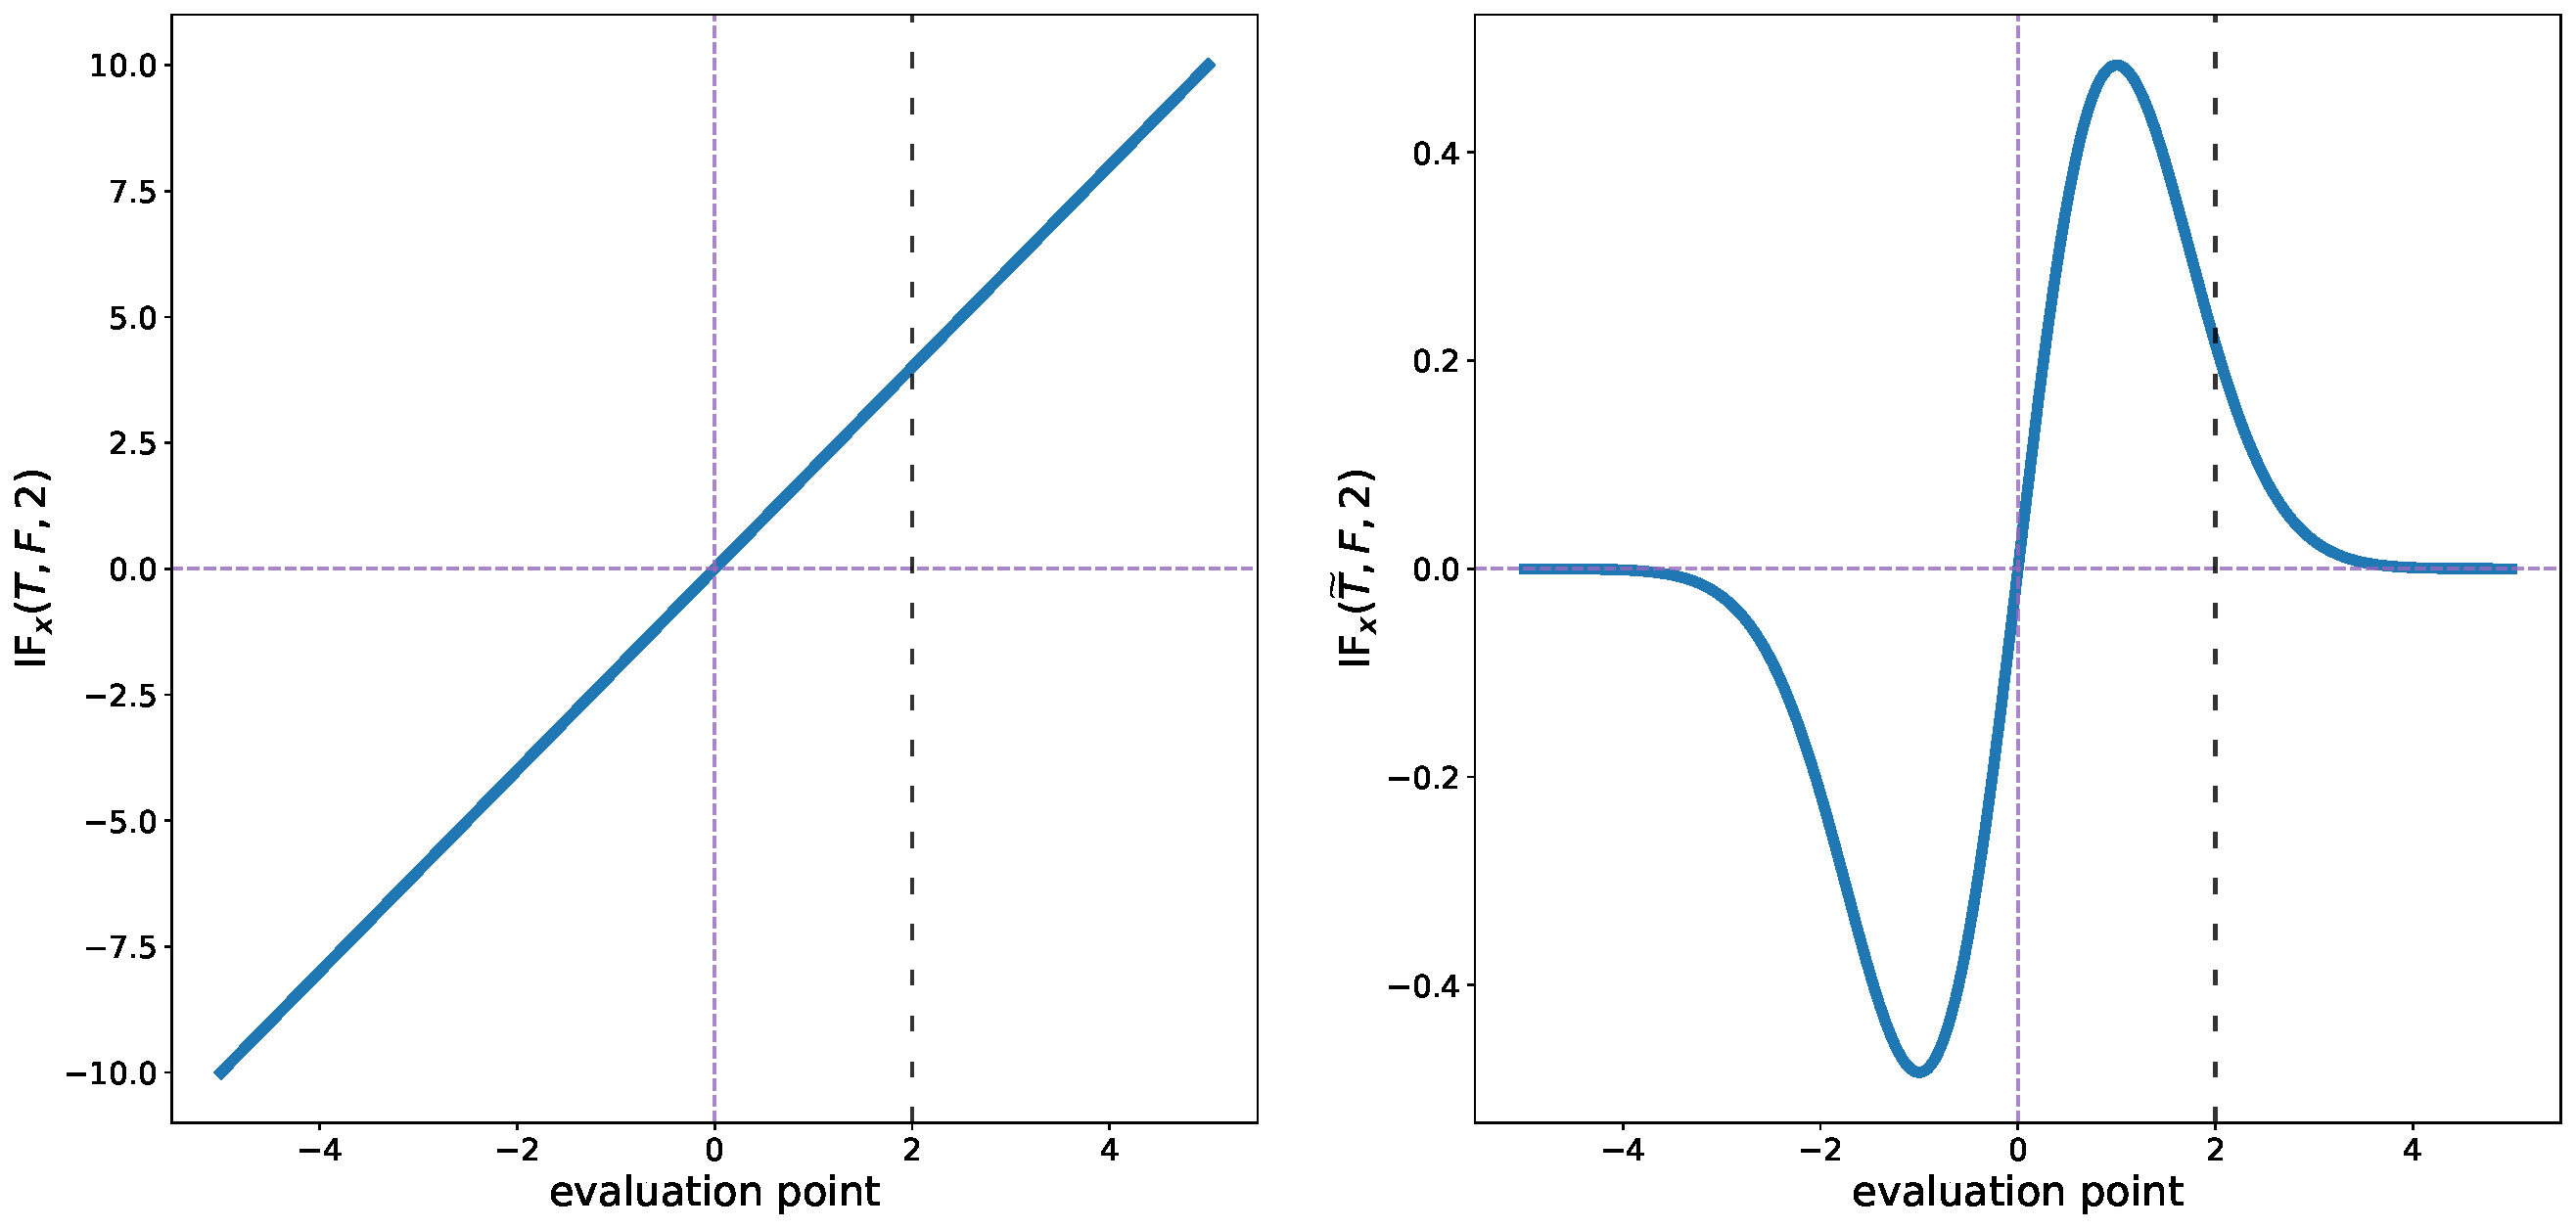
\includegraphics[width=\textwidth]{../plots/comparison-inffunden-inffunlogden-normal-loc-model-mean=0.0-y=2.0.pdf}
	\caption{$\mathrm{IF}_x \parens{T, F, y}$ (left panel) and $\mathrm{IF}_x \parens{\widetilde{T}, F, y}$ (right panel) evaluated at different $x \in \calX$ with $\E_F \bracks{X} = 0$ and $y = 2$. The black dashed vertical line indicates the location of the contaminant $y$. }
	\label{fig-inffun-logden-den-normal-loc-model}
\end{figure}

If we fix $y$ and $F$ and view $\mathrm{IF}_x \parens{T, F, y}$ and $\mathrm{IF}_x \parens{\widetilde{T}, F, y}$ as functions of the evaluation point $x$, both can vary with $x$, which is obvious from Figure \ref{fig-inffun-logden-den-normal-loc-model}. In other words, with a fixed $F$, a fixed $y$ can have different effects on each of $T \parens{F}$ and $\widetilde{T} \parens{F}$ at different evaluation points. In order to have a summarizing quantity to describe the maximal possible effect of $y$ on $T \parens{F}$ and $\widetilde{T} \parens{F}$, we use 
\begin{align*}
	M \parens{T, F, y} := \sup_{x \in \calX} \abs{\mathrm{IF}_x \parens{T, F, y}}, \qquad \text{ and } \qquad
	M \parens{\widetilde{T}, F, y} := \sup_{x \in \calX} \abs{\mathrm{IF}_x \parens{\widetilde{T}, F, y}}, 
\end{align*}
and call them the \textit{overall influences} of $y$ on $T \parens{F}$ and $\widetilde{T} \parens{F}$, respectively. They describe the maximal possible effects of $y$ on $T \parens{F}$ and $\widetilde{T} \parens{F}$, respectively. 

\renewcommand\thmcontinues[1]{continued}
\begin{example}[name=Normal location model, continues=example-normal-loc-model]
	The overall influences of $y$ on $T \parens{F}$ and $\widetilde{T} \parens{F}$ are 
	\begin{align*}
		M \parens{T, F, y} = & \, \begin{cases}
			0, & \, \text{ if } y = \E_F \bracks{X} \\ 
			\infty, & \, \text{ if } y \neq \E_F \bracks{X}
		\end{cases}, \quad \text{ and } \quad 
		M \parens{\widetilde{T}, F, y} = \frac{1}{\sqrt{2 e \pi}} \big\vert y - \E_F \bracks{X} \big\vert, 
	\end{align*}
	respectively. 
	
	Note that, when $y \neq \E_F \bracks{X}$, the overall influence of $y$ on $T \parens{F}$ is infinite, even though the density estimates appear indistinguishable. This infinite overall influence occurs at the two tails by noting $\lim_{x \to \pm \infty} \abs{\mathrm{IF}_x \parens{T, F, y}} = \infty$. This is a potential deficiency of defining the overall influence of $y$ on $T \parens{F}$ to be the supremum norm of $\mathrm{IF}_x \parens{T, F, y}$ taken with respect to the evaluation point $x \in \calX$. 
% the main reason that we have an infinite overall influence is . In other words, this infinite supremum norm occurs at the two tails. This infinite overall influence does \textit{not} imply that log-denisty functions $T \parens{F}$ and $T \parens{\parens{1 - \varepsilon} F + \varepsilon \delta_y}$ are significantly different for an infinitesimal $\varepsilon > 0$, or that denisty functions $\widetilde{T} \parens{F}$ and $\widetilde{T} \parens{\parens{1 - \varepsilon} F + \varepsilon \delta_y}$ are significantly different for an infinitesimal $\varepsilon > 0$. In general, it may \textit{not} be very meaningful to look at an infinite overall influence that occurs at the tails. 
\end{example}

Finally, we define the \textit{sample influence functions of $T \parens{F}$ and $\widetilde{T} \parens{F}$ evaluated at $x \in \calX$} to be 
\begin{align*}
	\mathrm{SIF}_{x, \varepsilon} \parens{T, F, y} := \frac{1}{\varepsilon} \parens[\Big]{T \parens[\big]{\parens{1 - \varepsilon} F + \varepsilon \delta_y} \parens{x} - T \parens{F} \parens{x}}, \\ 
	\mathrm{SIF}_{x, \varepsilon} \parens{\widetilde{T}, F, y} := \frac{1}{\varepsilon} \parens[\Big]{\widetilde{T} \parens[\big]{\parens{1 - \varepsilon} F + \varepsilon \delta_y} \parens{x} - \widetilde{T} \parens{F} \parens{x}}, 
\end{align*}
respectively, and the corresponding \textit{sample overall influences} to be 
\begin{align*}
	\widehat{M}_{\varepsilon} \parens{T, F, y} := \sup_{x \in \calX} \abs{\mathrm{SIF}_{x, \varepsilon} \parens{T, F, y}}, \qquad \text{ and } \qquad
	\widehat{M}_{\varepsilon} \parens{\widetilde{T}, F, y} := \sup_{x \in \calX} \abs{\mathrm{SIF}_{x, \varepsilon} \parens{\widetilde{T}, F, y}}
\end{align*}
respectively. Similarly to \eqref{eq-sample-inffun}, $\mathrm{SIF}_{x, \varepsilon} \parens{T, F, y}$ (\textit{resp.} $\mathrm{SIF}_{x, \varepsilon} \parens{\widetilde{T}, F, y}$) is the finite-difference approximation of $\mathrm{IF}_{x} \parens{T, F, y}$ (\textit{resp.} $\mathrm{IF}_{x, \varepsilon} \parens{\widetilde{T}, F, y}$). 


%The only issue that makes this unusual from the usual definition of an influence function is that you are considering function-valued maps $T$. 
%
%Let $T$ be a map from distributions $F$ on $\calX$ to a function on $\calX$. The influence function is defined to be: $\mathrm{IF} (x; T; F)$
%
%Note that this influence function is itself \textit{function-valued}. We will be using this to study the sensitivity of log-density estimators $T$. So $\mathrm{IF} (x; T; F)$ tells us how the log-density is affected by $x$. 
%
%As I said, the main issue that makes this unusual is that $\mathrm{IF} (x; T; F)$ is function-valued. 
%Overall influence::
%Define $| |$ to be sup norm of functions on $\calX$. Overall influence function: 
%$OIF(x; T; F) = | IF(x; T; F) |$ 


\section{Influence Functions of Density Projections in a Finite-dimensional Exponential Family}\label{section-influence-function-fin-dim-exp-fam}

With the introduction of $\mathrm{IF}_x \parens{T, F, y}$ and $\mathrm{IF}_x \parens{\widetilde{T}, F, y}$ in the preceding section, we focus on the influence functions of the ML and SM density projections (to be defined later) in an $m$-dimensional exponential family $\calQ_{\mathrm{fin}}$ (introduced in Chapter \ref{ch2}) in this section. 

Recall $\calQ_{\mathrm{fin}}$ contains all pdfs of the form 
\begin{align*}
	\tilde{q}_{\theta} \parens{x} := \mu \parens{x} \exp \parens[\big]{\innerp{\theta}{ \varphi \parens{x}} - B \parens{\theta}} \text{ for all } x \in \calX, \qquad \theta \in \Theta, 
\end{align*}
where we assume each component of $\varphi$, $\varphi_j: \calX \to \Real$, is twice continuously differentiable. We define the following maps 
\begin{align*}
	T \parens{F} = & \, \log \tilde{q}_{\theta_{\ML, F}},  && \, \text{ and }  && \, S \parens{F} = \log \tilde{q}_{\theta_{\SM, F}}, \\ 
	\widetilde{T} \parens{F} = & \, \tilde{q}_{\theta_{\ML, F}},  && \, \text{ and } && \, \widetilde{S} \parens{F} = \tilde{q}_{\theta_{\SM, F}}, 
\end{align*}
where $F$ is a distribution function over $\calX$, 
\begin{align*}
	\theta_{\ML, F} := & \, \argmin_{\theta \in \Theta} \braces[\Bigg]{ \int_{\calX} - \log \tilde{q}_{\theta} \parens{x} \mathrm{d} F \parens{x} } \\ 
	= & \, \argmin_{\theta \in \Theta} \braces[\Bigg]{ B \parens{\theta} - \innerp[\Big]{\theta}{ \E_F \bracks{ \varphi \parens{X} } } }, \\ 
	\theta_{\SM, F} := & \, \argmin_{\theta \in \Theta} \braces[\Bigg]{ \int_{\calX} \sum_{u=1}^d \parens[\bigg]{ \frac{1}{2} \parens[\big]{ \partial_u \log \tilde{q}_{\theta} \parens{x}}^2 + \partial_u \log \tilde{q}_{\theta} \parens{x} } \diff F \parens{x} } \\ 
	= & \, \argmin_{\theta \in \Theta} \braces[\Bigg]{ \frac{1}{2} \theta^\top \E_F \bracks{D_1 \parens{X} D_1 \parens{X}^\top } \theta - \theta^\top \E_F \bracks{W \parens{X}}}, 
\end{align*}
$D_1$ is a map from $\calX$ to $\Real^{m \times d}$ with $\bracks{D_1 \parens{x}}_{j, u} = \partial_u \varphi_j \parens{x}$ for all $x \in \calX$, $D_2$ is a map from $\calX$ to $\Real^{m \times d}$ with $\bracks{D_2 \parens{x}}_{j, u} = \partial_u^2 \varphi_j \parens{x}$ for all $x \in \calX$, $W$ is a map from $\calX$ to $\Real^m$ with $W \parens{x} = - \parens{ D_1 \parens{x} \nabla \log \mu \parens{x} + D_2 \parens{x} \boldone_d}$ for all $x \in \calX$, and $\boldone_d := \parens{1, \cdots, 1}^\top \in \Real^d$. Supposing that the pdf of $F$, denoted by $p_0$, exists, we observe that $\widetilde{T} \parens{F}$ and $\widetilde{S} \parens{F}$ are the ML and SM density projections of $p_0$ onto the family $\calQ_{\mathrm{fin}}$, as they have the smallest KL- and H-divergences to $p_0$ among all $\tilde{q}_{\theta} \in \calQ_{\mathrm{fin}}$, respectively. 

Then, the following theorem provides explicit expressions for $\mathrm{IF}_x \parens{T, F, y}$ and $\mathrm{IF}_x \parens{S, F, y}$. The expressions for $\mathrm{IF}_x \parens{\widetilde{T}, F, y}$ and $\mathrm{IF}_x \parens{\widetilde{S}, F, y}$ are easy to obtain by multiplying $\mathrm{IF}_x \parens{T, F, y}$ and $\mathrm{IF}_x \parens{S, F, y}$ with $\widetilde{T} \parens{F} \parens{x}$ and $\widetilde{S} \parens{F} \parens{x}$, respectively, using Proposition \ref{prop-inf-fun-relationship-den-logden}. 

\begin{theorem}[Influence functions of ML and SM log-density projections in $\calQ_{\mathrm{fin}}$ evaluated at $x \in \calX$]\label{theorem-inf-fun-ml-sm-fin-dim-exp-fam}
	\leavevmode
	\begin{enumerate}[label=(\alph*)]
		\item \label{theorem-inf-fun-ml-sm-fin-dim-exp-fam-a} Assume $\E_F \bracks{\varphi \parens{X}}$ exists and belongs to $\interior \parens{\Theta}$, $\int_{\calX} \tilde{q}_{\theta_{\ML, F}} \parens{x} \norm{\varphi \parens{x}}_2^2 \diff x < \infty$, and $\nabla^2 B \parens{\theta_{\ML, F}}$ is invertible. Then, for all $x \in \calX$, 
		\begin{align}\label{eq-inffun-ml-fin-dim-exp-fam}
			\mathrm{IF}_x \parens{T, F, y} = \innerp[\Bigg]{ \widetilde{G}_{\ML} \parens{F, y} }{ \varphi \parens{x} - \int_{\calX} \tilde{q}_{\theta_{\ML, F}} \parens{w} \varphi \parens{w} \diff w }, 
		\end{align}
		where 
		\begin{align*}
			\widetilde{G}_{\ML} \parens{F, y} := \bracks[\big]{\nabla^2 B \parens{\theta_{\ML, F} }}^{-1} \parens[\big]{\varphi \parens{y} - \E_{F} \bracks{\varphi \parens{X}}}
		\end{align*}
		
		\item \label{theorem-inf-fun-ml-sm-fin-dim-exp-fam-b} Assume $\E_F \bracks{W \parens{X}}$ exists, $\int_{\calX} \tilde{q}_{\theta_{\SM, F}} \parens{x} \norm{\varphi \parens{x}}_2^2 \diff x < \infty$, and $\E_F \bracks[\big]{D_1 \parens{X} D_1 \parens{X}^\top}$ is invertible. Then, for all $x \in \calX$, 
		\begin{align}\label{eq-inffun-sm-fin-dim-exp-fam}
			\mathrm{IF}_x \parens{T, F, y} = & \, \innerp[\bigg]{ \widetilde{G}_{\SM} \parens{F, y}}{ \varphi \parens{x} - \int_{\calX} \tilde{q}_{\theta_{\SM, F}} \parens{w} \varphi \parens{w} \diff w}, 
		\end{align}
		where 
		\begin{align*}
			\widetilde{G}_{\SM} \parens{F, y} := & \, \bracks[\Big]{\E_F \bracks[\big]{D_1 \parens{X} D_1 \parens{X}^\top} }^{-1} \times \\ 
			& \qquad \qquad  \braces[\bigg]{W  \parens{y} - D_1 \parens{y} D_1 \parens{y}^\top \bracks[\Big]{\E_F \bracks[\big]{D_1 \parens{X} D_1 \parens{X}^\top} }^{-1} \E_F \bracks{W \parens{X}} }. 
		\end{align*}
	\end{enumerate}
\end{theorem}

The proof of Theorem \ref{theorem-inf-fun-ml-sm-fin-dim-exp-fam} will be provided in Section \ref{proof-theorem-inf-fun-ml-sm-fin-dim-exp-fam}. 

From the proof, we can see $\widetilde{G}_{\ML} \parens{F, y}$ is the influence function of the $M$-estimator $\theta_{\ML, F}$ that satisfies 
\begin{align*}
	0 = \int_{\calX} \parens[\Big]{\nabla B \parens{\theta_{\ML, F}} - \varphi \parens{x}} \diff F \parens{x}, 
\end{align*}
and $\widetilde{G}_{\SM} \parens{F, y}$ is the influence function of the $M$-estimator $\theta_{\SM, F}$ that satisfies 
\begin{align*}
	0 = \E_F \bracks[\big]{D_1 \parens{X} D_1 \parens{X}^\top} \theta_{\SM, F} - \E_F \bracks{W \parens{X}}; 
\end{align*}
in other words, they are the influence functions of their respective natural parameters. % By inspecting the form of \eqref{eq-inffun-ml-fin-dim-exp-fam} and \eqref{eq-inffun-sm-fin-dim-exp-fam}, we see each of them is the inner product between the influence function of the natural parameter and the derivative of the log-density function with respect to $\theta$ evaluated at the unperturbed natural parameter. 

Comparing \eqref{eq-inffun-ml-fin-dim-exp-fam} and \eqref{eq-inffun-sm-fin-dim-exp-fam}, we see that $\mathrm{IF}_x \parens{T, F, y}$ depends on $y$ \emph{only} through the canonical statistics $\varphi$, but $\mathrm{IF}_x \parens{S, F, y}$ depends on $y$ through the first two derivatives of $\varphi$ and the first derivative of $\log \mu$. This is the key difference between $\mathrm{IF}_x \parens{T, F, y}$ and $\mathrm{IF}_x \parens{S, F, y}$. In the examples we will see later, their differences will become more apparent. 

From Theorem \ref{theorem-inf-fun-ml-sm-fin-dim-exp-fam}, we can obtain some properties of $\mathrm{IF}_x \parens{T, F, y}$ and $\mathrm{IF}_x \parens{S, F, y}$ which are given in the corollaries below. 

\begin{corollary}\label{corollary-inffun-fin-dim-exp-fam-zero}
	\leavevmode
	\begin{enumerate}[label=(\alph*)]
		\item \label{corollary-inffun-fin-dim-exp-fam-zero-a} Under the assumptions in Theorem \ref{theorem-inf-fun-ml-sm-fin-dim-exp-fam}\ref{theorem-inf-fun-ml-sm-fin-dim-exp-fam-a}, $\mathrm{IF}_x \parens{T, F, y} = 0$ for all $x \in \calX$ if and only if $F$ and $y$ satisfy 
		\begin{align}\label{eq-corollary-inffun-fin-dim-exp-fam-zero-a}
			\varphi \parens{y} - \E_F \bracks{\varphi \parens{X}} = 0. 
		\end{align} 
		
		\item \label{corollary-inffun-fin-dim-exp-fam-zero-b} Under the assumptions in Theorem \ref{theorem-inf-fun-ml-sm-fin-dim-exp-fam}\ref{theorem-inf-fun-ml-sm-fin-dim-exp-fam-b}, $\mathrm{IF}_x \parens{S, F, y} = 0$ for all $x \in \calX$ if and only if $F$ and $y$ satisfy 
		\begin{align}\label{eq-corollary-inffun-fin-dim-exp-fam-zero-b}
			W \parens{y} - D_1 \parens{y} D_1 \parens{y}^\top \bracks[\Big]{\E_F \bracks[\big]{D_1 \parens{X} D_1 \parens{X}^\top} }^{-1} \E_F \bracks{W \parens{X}} = 0. 
		\end{align}
	\end{enumerate}
\end{corollary}

\begin{corollary}\label{corollary-inffun-fin-dim-exp-fam-bounded}
	\leavevmode
	\begin{enumerate}[label=(\alph*)]
		\item \label{corollary-inffun-fin-dim-exp-fam-bounded-a} Under the assumptions in Theorem \ref{theorem-inf-fun-ml-sm-fin-dim-exp-fam}\ref{theorem-inf-fun-ml-sm-fin-dim-exp-fam-a}, suppose $F$ and $y$ satisfy $\varphi \parens{y} - \E_F \bracks{\varphi \parens{X}} \neq 0$. 
		\begin{enumerate}[label=(\roman*)]
			\item If $\sup_{j = 1, \cdots, m} \ \sup_{x \in \calX} \abs{\varphi_j \parens{x}} < \infty$, then $M \parens{T, F, y} < \infty$. 
			\item If there exists $j^* \in \sets{1, \cdots, m}$ and $x_0 \in \overline{\calX}$ such that $\lim_{x \to x_0} \abs{\varphi_{j^*} \parens{x}} = \infty$ so that $\sup_{x \in \calX} \abs{\varphi_j \parens{x}} = \infty$, $\varphi_{j^*} \parens{y} - \E_F \bracks{\varphi_{j^*} \parens{X}} \neq 0$, and $\lim_{x \to x_0} \frac{\varphi_j \parens{x}}{\varphi_{j^*} \parens{x}} = 0$ for all $j \neq j^*$, then $M \parens{T, F, y} = \infty$. 
		\end{enumerate}
		
		\item \label{corollary-inffun-fin-dim-exp-fam-bounded-b} Under the assumptions in Theorem \ref{theorem-inf-fun-ml-sm-fin-dim-exp-fam}\ref{theorem-inf-fun-ml-sm-fin-dim-exp-fam-b}, suppose $F$ and $y$ satisfy 
		\begin{align*}
			W \parens{y} - D_1 \parens{y} D_1 \parens{y}^\top \bracks[\Big]{\E_F \bracks[\big]{D_1 \parens{X} D_1 \parens{X}^\top} }^{-1} \E_F \bracks{W \parens{X}} \neq 0. 
		\end{align*}
		\begin{enumerate}[label=(\roman*)]
			\item If $\sup_{j = 1, \cdots, m} \ \sup_{x \in \calX} \abs{\varphi_j \parens{x}} < \infty$, then $M \parens{S, F, y} < \infty$. 
			\item If there exists $j^* \in \sets{1, \cdots, m}$ and $x_0 \in \overline{\calX}$ such that $\lim_{x \to x_0} \abs{\varphi_{j^*} \parens{x}} = \infty$ so that $\sup_{x \in \calX} \abs{\varphi_j \parens{x}} = \infty$, the $j^*$-th element of 
			\begin{align*}
				W \parens{y} - D_1 \parens{y} D_1 \parens{y}^\top \bracks[\Big]{\E_F \bracks[\big]{D_1 \parens{X} D_1 \parens{X}^\top} }^{-1} \E_F \bracks{W \parens{X}}
			\end{align*}
			is nonzero, and $\lim_{x \to x_0} \frac{\varphi_j \parens{x}}{\varphi_{j^*} \parens{x}} = 0$ for all $j \neq j^*$, then $M \parens{S, F, y} = \infty$. 
		\end{enumerate}
	\end{enumerate}
\end{corollary}

These corollaries are obvious from Theorem \ref{theorem-inf-fun-ml-sm-fin-dim-exp-fam}, in particular, from \eqref{eq-inffun-ml-fin-dim-exp-fam} and \eqref{eq-inffun-sm-fin-dim-exp-fam}, and their proofs are omitted here. In the rest of this section, we provide several examples to illustrate Theorem \ref{theorem-inf-fun-ml-sm-fin-dim-exp-fam} and Corollaries \ref{corollary-inffun-fin-dim-exp-fam-zero} and \ref{corollary-inffun-fin-dim-exp-fam-bounded}. 

\begin{example}[name=Normal location-scale model]
	Let $\calX = \Real$ and $\calQ$ contain all pdfs of the form 
	\begin{align*}
		\tilde{q}_{\theta} \parens{x} := \frac{1}{\sqrt{2 \pi \sigma^2}} \exp \parens[\bigg]{- \frac{\parens{x - \omega}^2}{2 \sigma^2}} \text{ for all } x \in \mathcal{X}, \qquad \theta := \parens{\omega, \sigma^2} \in \Theta, 
	\end{align*}
	where $\Theta := \mathbb{R} \times \parens{0, \infty}$. In this example, we have 
	\begin{align*}
		\mu \parens{x} = \frac{1}{\sqrt{2 \pi}}, \qquad \varphi \parens{x} = \begin{pmatrix}
			x \\ x^2
		\end{pmatrix}, \qquad B \parens{\theta} = \frac{\omega^2}{2 \sigma^2} + \frac{1}{2} \log \sigma^2, 
	\end{align*}
	and 
	\begin{align*}
		D_1 \parens{x} = \begin{pmatrix}
			1 \\ 2x
		\end{pmatrix}, \qquad D_2 \parens{x} = \begin{pmatrix}
			0 \\ 2
		\end{pmatrix}, \qquad \parens{\log \mu}' \parens{x} = 0, \qquad  W \parens{x} = \begin{pmatrix}
			0 \\ -2
		\end{pmatrix}. 
	\end{align*}
	Assume $m_1 := \E_F \bracks{X}$ and $m_2 := \E_F \bracks{X^2}$ both exist and $m_2 - m_1^2 > 0$. Then, using Theorem \ref{theorem-inf-fun-ml-sm-fin-dim-exp-fam}, we have 
	\begin{align*}
		\mathrm{IF}_x \parens{T, F, y} = & \, \mathrm{IF}_x \parens{S, F, y} = a_1 x^2 + a_2 x + a_3, \qquad \text{ for all } x \in \calX, 
	\end{align*}
	where 
	\begin{align*}
		a_1 := & \, \frac{-m_1}{\parens{m_2 - m_1^2}^2} \parens{y - m_1} + \frac{1}{2 \parens{m_2 - m_1^2}^2} \parens{y^2 - m_2}, \\
		a_2 := & \, \frac{m_2 + m_1^2}{\parens{m_2 - m_1^2}^2} \parens{y - m_1} - \frac{m_1}{\parens{m_2 - m_1^2}^2} \parens{y^2 - m_2}, \\ 
		a_3 := & \, \frac{m_1^3 - 2 m_1 m_2}{\parens{m_2 - m_1^2}^2} \parens{y - m_1} + \frac{m_2}{2 \parens{m_2 - m_1^2}^2} \parens{y^2 - m_2}. 
	\end{align*}
	
	Since, in this example, we have $\varphi_1 \parens{x} = x$ and $\varphi_2 \parens{x} = x^2$ for all $x \in \calX$, and $\sup_{x \in \calX} \vert \varphi_2 \parens{x} \vert = \infty$ with $\lim_{x \to \pm \infty} \varphi_2 \parens{x} = \infty$, and $\lim_{x \to \pm \infty} \frac{\varphi_1 \parens{x}}{\varphi_2 \parens{x}} = 0$, we have $M \parens{T, F, y} = M \parens{S, F, y} = \infty$, which verifies Corollary \ref{corollary-inffun-fin-dim-exp-fam-bounded}. 
	% If $m_1 \neq y$ or $m_2 \neq y^2$, we have 
%	and 
%	\begin{align*}
%		\mathrm{IF}_x \parens{\widetilde{T}, F, y} = & \, \mathrm{IF}_x \parens{\widetilde{S}, F, y} = \tilde{q}_{\parens{m_1, m_2 - m_1^2}} \parens{x} \parens{a_1 x^2 + a_2 x + a_3}, \qquad \text{ for all } x \in \calX, \\ 
%		M \parens{\widetilde{T}, F, y} = & \, M \parens{\widetilde{S}, F, y} =  , 
%	\end{align*}
\end{example}


\begin{example}[name=Lognormal location model]
	Let $\mathcal{X} = \parens{0, \infty}$ and $\calQ$ contain all pdfs of the form 
	\begin{align*}
		\tilde{q}_{\theta} \parens{x} := \frac{1}{x \sqrt{2 \pi}} \exp \parens[\bigg]{- \frac{\parens{\log x - \theta}^2}{2}} \text{ for all } x \in \calX, \qquad \theta \in \Real. 
	\end{align*}
	In this example, we have 
	\begin{align*}
		\mu \parens{x} = \frac{1}{x \sqrt{2 \pi}} \exp \parens[\bigg]{- \frac{\parens{\log x}^2}{2}}, \qquad \varphi \parens{x} = \log x, \qquad B \parens{\theta} = \frac{\theta^2}{2}, 
	\end{align*}
	and 
	\begin{align*}
		D_1 \parens{x} = \frac{1}{x}, \quad D_2 \parens{x} = - \frac{1}{x^2}, \quad \parens{\log \mu}' \parens{x} = -\frac{1}{x} - \frac{\log x}{x}, \quad W \parens{x} = \frac{2}{x^2} + \frac{\log x}{x^2}. 
	\end{align*}
	Then, using Theorem \ref{theorem-inf-fun-ml-sm-fin-dim-exp-fam}, we obtain 
	\begin{align*}
		\mathrm{IF}_x \parens{T, F, y} = & \, \parens[\big]{\log y - m_1 } \parens[\big]{\log x - m_1 }, \\ 
		\mathrm{IF}_x \parens{S, F, y} = & \, \frac{1}{m_3 y^2} \parens[\bigg]{\log y - \frac{m_2}{m_3}} \parens[\bigg]{\log x - 2 - \frac{m_2}{m_3}}, 
	\end{align*}
	for all $x \in \calX$, where we assume $m_1 := \E_F \bracks{\log X}$, $m_2 := \E_F \bracks{X^{-2} \log X}$ and $m_3 := \E_F \bracks{X^{-2}}$ exist. 
	
	In particular, $\mathrm{IF}_x \parens{T, F, y} = 0$ for all $x \in \calX$ if and only if $F$ and $y$ satisfy $\log y = m_1$, which is exactly \eqref{eq-corollary-inffun-fin-dim-exp-fam-zero-a}; and, $\mathrm{IF}_x \parens{S, F, y} = 0$ for all $x \in \calX$ if and only if $F$ and $y$ satisfy $\log y - \frac{m_2}{m_3} = 0$, which is exactly \eqref{eq-corollary-inffun-fin-dim-exp-fam-zero-b}. These illustrate Corollary \ref{corollary-inffun-fin-dim-exp-fam-zero}. 
	
	Also, note that, in this example, $\sup_{x \in \calX} \abs{\varphi \parens{x}} = \sup_{x \in \calX} \abs{\log x} = \infty$. Supposing $\log y - \E_F \bracks{\log X} \neq 0$, we have $M \parens{T, F, y} = \infty$, which illustrates Corollary \ref{corollary-inffun-fin-dim-exp-fam-bounded}\ref{corollary-inffun-fin-dim-exp-fam-bounded-a}; supposing $\log y - \frac{m_2}{m_3} \neq 0$, we have $M \parens{S, F, y} = \infty$, which illustrates Corollary \ref{corollary-inffun-fin-dim-exp-fam-bounded}\ref{corollary-inffun-fin-dim-exp-fam-bounded-b}. 
%	For fixed $x \in \calX$ and $F$, the larger the value of $y$ is, the larger the value of $\mathrm{IF}_x \parens{T, F, y}$ is. 
%	For fixed $x \in \calX$ and $F$, 
%	\begin{itemize}
%		\item if $y \in \parens[\Big]{0, \exp \parens[\big]{\frac{m_1}{m_2} + \frac{1}{2}}}$, the larger $y$ is, the larger $\mathrm{IF}_x \parens{S, F, y}$ is; 
%		\item if $y > \exp \parens[\big]{\frac{m_1}{m_2} + \frac{1}{2}}$, the larger $y$ is, the smaller $\mathrm{IF}_x \parens{S, F, y}$ is. 
%	\end{itemize}
\end{example}


\begin{example}[name=Gamma rate model]
	Let $\calX = \parens{0, \infty}$ and $\calQ$ contain all pdfs of the form 
	\begin{align*}
		\tilde{q}_{\theta} \parens{x} := \frac{x^{\alpha-1}}{\Gamma \parens{\alpha}} \exp \parens[\Big]{- \theta x + \alpha \log \theta} \text{ for all } x \in \calX, \qquad \theta \in \parens{0, \infty}. 
	\end{align*}
	We assume $\alpha > 1$ is known. In this example 
	\begin{align*}
		\mu \parens{x} = \frac{x^{\alpha-1}}{\Gamma \parens{\alpha}}, \qquad \varphi \parens{x} = - x, \qquad B \parens{\theta} = - \alpha \log \theta, 
	\end{align*}
	and 
	\begin{align*}
		D_1 \parens{x} = -1, \quad D_2 \parens{x} = 0, \quad \parens{\log \mu}' \parens{x} = \frac{\alpha - 1}{x}, \quad W \parens{x} = \frac{\alpha - 1}{x}. 
	\end{align*}
	Then, using Theorem \ref{theorem-inf-fun-ml-sm-fin-dim-exp-fam}, we obtain 
	\begin{align*}
		\mathrm{IF}_x \parens{T, F, y} = & \, \frac{\alpha}{m_1^2} \parens{y - m_1} \parens{x - m_1}, \\ 
		\mathrm{IF}_x \parens{S, F, y} = & \, \parens{\alpha - 1} \parens{m_2 - y^{-1} } \parens[\bigg]{x - \frac{\alpha}{\alpha - 1} \frac{1}{m_2}}, 
	\end{align*}
	for all $x \in \calX$, where we assume $m_1 := \E_F \bracks{X}$ and $m_2 := \E_F \bracks{X^{-1}}$ exist. 
	
	In particular, $\mathrm{IF}_x \parens{T, F, y} = 0$ for all $x \in \calX$ if and only if $F$ and $y$ satisfy $y = m_1$, which is exactly \eqref{eq-corollary-inffun-fin-dim-exp-fam-zero-a}; and, $\mathrm{IF}_x \parens{S, F, y} = 0$ for all $x \in \calX$ if and only if $F$ and $y$ satisfy $y^{-1} - m_2 = 0$, which is exactly \eqref{eq-corollary-inffun-fin-dim-exp-fam-zero-b}. These illustrate Corollary \ref{corollary-inffun-fin-dim-exp-fam-zero}. 
	
	Note that, in this example, $\sup_{x \in \calX} \abs{\varphi \parens{x}} = \sup_{x \in \calX} \abs{-x} = \infty$. Supposing $\E_F \bracks{X} - y \neq 0$, we have $M \parens{T, F, y} = \infty$, which illustrates Corollary \ref{corollary-inffun-fin-dim-exp-fam-bounded}\ref{corollary-inffun-fin-dim-exp-fam-bounded-a}; supposing $m_2 - y^{-1} \neq 0$, we have $M \parens{S, F, y} = \infty$, which illustrates Corollary \ref{corollary-inffun-fin-dim-exp-fam-bounded}\ref{corollary-inffun-fin-dim-exp-fam-bounded-b}. 
%	For fixed $x \in \calX$ and $F$, the larger the value of $y$ is, the larger the value of $\mathrm{IF}_x \parens{T, F, y}$ is. 
%	For fixed $x \in \calX$ and $F$, the larger the value of $y$ is, the larger the value of $\mathrm{IF}_x \parens{S, F, y}$ is. 
\end{example}

\section{Influence Functions of Density Projections in a Kernel Exponential Family}\label{section-influence-function-kernel-exp-fam}

We now turn to the influence functions of the ML and SM density projections in a kernel exponential family $\calQ_{\ker}$ (introduced in Chapter \ref{ch2}) in this section. Recall $\calQ_{\ker}$ contains all pdfs of the form 
\begin{align*}
	q_{f} \parens{x} := \mu \parens{x} \exp \parens[\big]{f \parens{x} - A \parens{f}} \text{ for all } x \in \calX, \qquad f \in \calF \subseteq \calH. 
\end{align*}

We still let $F$ be a distribution function over $\calX$, and define the following maps 
\begin{align*}
	T_{\lambda} \parens{F} = & \, \log q_{f_{\ML, F}^{\parens{\lambda}}},  && \, \text{ and }  && \, S_{\rho} \parens{F} = \log q_{f_{\SM, F}^{\parens{\rho}}}, \\ 
	\widetilde{T}_{\lambda} \parens{F} = & \, q_{f_{\ML, F}^{\parens{\lambda}}},  && \, \text{ and }  && \, \widetilde{S}_{\rho} \parens{F} = q_{f_{\SM, F}^{\parens{\rho}}}, 
\end{align*}
where 
\begin{align}
	f_{\ML, F}^{\parens{\lambda}} := & \, \argmin_{f \in \calF} \braces[\Bigg]{A \parens{f} - \int_{\calX} f \parens{x} \diff F \parens{x} + \frac{\lambda}{2} \norm{f}_{\calH}^2}, \label{eq-ml-obj-fun-general} \\ 
	f_{\SM, F}^{\parens{\rho}} := & \, \argmin_{f \in \calF} \braces[\Bigg]{\frac{1}{2} \innerp{f}{C_{F} f}_{\calH} - \innerp{f}{z_{F}}_{\calH} + \frac{\rho}{2} \norm{f}_{\calH}^2}, \label{eq-sm-obj-fun-general}
\end{align}
with $C_F := \int_{\calX} \sum_{u=1}^d \partial_u k \parens{x, \,\cdot\,} \otimes \partial_u k \parens{x, \,\cdot\,} \diff F \parens{x}$ mapping from $\calH$ to $\calH$, and $z_F := - \int_{\calX} \sum_{u=1}^d \parens{\partial_u \log \mu \parens{x} \partial_u k \parens{x, \,\cdot\,} + \partial_u^2 k \parens{x, \,\cdot\,}} \diff F \parens{x} \in \calH$. If the distribution function $F$ has a pdf $p_0$, the resulting $C_F$ is \eqref{eq-C-def} defined in Chapter \ref{ch3}; if $F = F_n$, the empirical distribution function of data $X_1, \cdots, X_n$, the resulting $C_{F_n}$ is $\widehat{C}$ defined in \eqref{eq-hatC} in Chapter \ref{ch2}. 

Note that both objective functionals in \eqref{eq-ml-obj-fun-general} and \eqref{eq-sm-obj-fun-general} are strongly convex with constants $\lambda > 0$ and $\rho > 0$, respectively. It follows that each of $f_{\ML, F}^{\parens{\lambda}}$ and $f_{\SM, F}^{\parens{\rho}}$ exists and is unique  \parencite[Corollary 11.17 in][]{Bauschke2017-he}. 

We then have the following results on the influence functions of the penalized ML and SM log-density projections onto $\calQ_{\ker}$ evaluated at $x \in \calX$. 

\begin{theorem}[Influence functions of ML and SM log-density projections in $\calQ_{\ker}$ evaluated at $x \in \calX$]\label{theorem-inf-fun-ml-sm-ker-exp-fam}
\leavevmode
	\begin{enumerate}[label=(\alph*)]
		\item \label{theorem-inf-fun-ml-sm-ker-exp-fam-a} Under \ref{assumption-2-1-inf-dim} - \ref{assumption-2-4-base-density} in Chapter \ref{ch2}, we have, for all $x \in \calX$, 
		\begin{align}\label{eq-inf-fun-ml-ker-exp-fam}
			\mathrm{IF}_x \parens{T_{\lambda}, F, y} = & \, \innerp[\Bigg]{G_{\ML} \parens{F, y}}{ k \parens{x, \,\cdot\,} - \int_{\calX} k \parens{w, \,\cdot\,} q_{f_{\ML, F}^{\parens{\lambda}}} \parens{w} \diff w }_{\calH}, 
		\end{align}
		where
		\begin{align*}
			G_{\ML} \parens{F, y} := & \, \Bigg\{\E_{q_{f_{\ML, F}^{\parens{\lambda}}}} \bracks[\Big]{ \parens[\big]{k \parens{X, \,\cdot\,} - \Upsilon } \otimes \parens[\big]{k \parens{X, \,\cdot\,} - \Upsilon }} + \lambda I \Bigg\}^{-1} \bigg( k \parens{y, \,\cdot\,} -  \\ 
			& \qquad \int_{\calX} k \parens{x, \,\cdot\,} \diff F \parens{x} \bigg) \in \calH, 
		\end{align*}
		and $\Upsilon := \int_{\calX} k \parens{x, \,\cdot\,} q_{f_{\ML, F}^{\parens{\lambda}}}\parens{x} \diff x \in \calH$. 
		
		\item \label{theorem-inf-fun-ml-sm-ker-exp-fam-b} Under \ref{assumption-2-1-inf-dim} - \ref{assumption-2-4-base-density} in Chapter \ref{ch2} and \ref{assumption-1} - \ref{assumption-5} in Chapter \ref{ch3}, we have, for all $x \in \calX$, 
		\begin{align}
			\mathrm{IF}_x \parens{S_{\rho}, F, y} = & \, \innerp[\Bigg]{G_{\SM} \parens{F, y}}{k \parens{x, \,\cdot\,} - \int_{\calX} k \parens{w, \,\cdot\,} q_{f_{\SM, F}^{\parens{\rho}}} \parens{w} \diff w}_{\calH}, 
		\end{align}
		where 
		\begin{align*}
			G_{\SM} \parens{F, y} := & \, \parens{C_{F} + \rho I}^{-1} \parens[\Big]{z_{\delta_y} - \parens{C_{\delta_y} + \rho I} \parens{C_{F} + \rho I}^{-1} z_{F}} \in \calH. 
		\end{align*}
	\end{enumerate}
\end{theorem}

The proof of Theorem \ref{theorem-inf-fun-ml-sm-ker-exp-fam} can be found in Section \ref{proof-theorem-inf-fun-ml-sm-ker-exp-fam}. 	

Comparing Theorems \ref{theorem-inf-fun-ml-sm-fin-dim-exp-fam} and \ref{theorem-inf-fun-ml-sm-ker-exp-fam}, we see they share many similarities. In particular, $\mathrm{IF}_x \parens{T_{\lambda}, F, y}$ depends on $y$ through $k$ \emph{only}, but $\mathrm{IF}_x \parens{S_{\rho}, F, y}$ depends on $y$ through the first two partial derivatives of $k$ and the first derivative of $\log \mu$. Moreover, $G_{\ML} \parens{F, y}$ is the influence function of the $M$-estimator $f_{\ML, F}^{\parens{\lambda}}$ that satisfies 
\begin{align*}
	0 = \int_{\calX} \parens[\Big]{\nabla A \parens{f_{\ML, F}^{\parens{\lambda}}} - k \parens{x, \,\cdot\,} + \lambda f_{\ML, F}^{\parens{\lambda}}} \diff F \parens{x}, 
\end{align*}
and $G_{\SM} \parens{F, y}$ is the influence function of the $M$-estimator $f_{\SM, F}^{\parens{\rho}}$ that satisfies 
\begin{align*}
	0 = C_F f_{\SM, F}^{\parens{\rho}} - z_{F} + \rho f_{\ML, F}^{\parens{\rho}}. 
\end{align*}
The covariance operator 
\begin{align*}
	\E_{q_{f_{\ML, F}^{\parens{\lambda}}}} \bracks[\Big]{ \parens[\big]{k \parens{X, \,\cdot\,} - \Upsilon } \otimes \parens[\big]{k \parens{X, \,\cdot\,} - \Upsilon }}
\end{align*}
appearing in $G_{\ML} \parens{F, y}$ plays the role of $\nabla^2 B \parens{\theta_{\ML, F} }$ in $\widetilde{G}_{\ML} \parens{F, y}$, where $\nabla^2 B \parens{\theta_{\ML, F} }$ is the covariance matrix of $\varphi$ under $\tilde{q}_{\theta_{\ML, F}}$. The operator $C_F$ appearing in $G_{\SM} \parens{F, y}$ plays the role of $\E_F \bracks{D_1 \parens{X} D_1 \parens{X}^{\top}}$ in $\widetilde{G}_{\SM} \parens{F, y}$, and $z_F$ in $G_{\SM} \parens{F, y}$ plays the role of $\E_F \bracks{W \parens{X}}$ in $\widetilde{G}_{\SM} \parens{F, y}$. 

Even though Theorem \ref{theorem-inf-fun-ml-sm-ker-exp-fam} provides explicit expressions of $\mathrm{IF}_x \parens{T_{\lambda}, F, y}$ and $\mathrm{IF}_x \parens{S_{\rho}, F, y}$, they are hard to work with directly to compare the sensitivities of the penalized ML and SM density estimators. We will work with the sample influence function in the next chapter and compare their sensitivities numerically. 

\newpage

\section{Proofs}

\subsection{Proof of Proposition \ref{prop-inf-fun-relationship-den-logden}}\label{proof-prop-inf-fun-relationship-den-logden}

\begin{proof}[Proof of Proposition \ref{prop-inf-fun-relationship-den-logden}]
	Under the assumption in the proposition and with an application of the chain rule, we have 
	\begin{align*}
		\mathrm{IF}_x \parens{\widetilde{T}, F, y} = & \, \frac{\diff}{\diff \varepsilon} \parens[\Big]{\widetilde{T} \parens[\big]{\parens{1 - \varepsilon} F + \varepsilon \delta_y} \parens{x} } \bigg\vert_{\varepsilon = 0} \\ 
		= & \, \frac{\diff}{\diff \varepsilon} \parens[\Big]{\exp \parens[\big]{T \parens{\parens{1 - \varepsilon} F + \varepsilon \delta_y} \parens{x} }} \bigg\vert_{\varepsilon = 0} \\ 
		= & \, \exp \parens[\big]{T \parens{F} \parens{x} } \frac{\diff}{\diff \varepsilon} \parens[\Big]{T \parens[\big]{\parens{1 - \varepsilon} F + \varepsilon \delta_y} \parens{x} } \bigg\vert_{\varepsilon = 0} \\ 
		= & \, \widetilde{T} \parens{F} \parens{x} \mathrm{IF}_x \parens{T, F, y}. 
	\end{align*}
\end{proof}


\subsection{Proof of Proposition \ref{prop-inf-fun-relationship-den-logden-kldiv}}\label{proof-prop-inf-fun-relationship-den-logden-kldiv}

\begin{proof}[Proof of Proposition \ref{prop-inf-fun-relationship-den-logden-kldiv}]
	Let $\varepsilon \in \parens{0, 1}$. By the definition of the KL-divergence, we have 
	\begin{align*}
		\mathrm{KL} \parens[\Big]{\widetilde{T} \parens{F} \big\Vert \widetilde{T} \parens{\parens{1 - \varepsilon} F + \varepsilon \delta_y}} = - \int_{\calX} \widetilde{T} \parens{F} \parens{x} \parens[\Big]{T \parens{ \parens{1 - \varepsilon} F + \varepsilon \delta_y} \parens{x} - T \parens{F} \parens{x} } \diff x. 
	\end{align*}
	Differentiating both sides wrt $\varepsilon$, interchanging differentiation and integral (which is allowed by the assumptions), and evaluating at $\varepsilon = 0$, we have 
	\begin{align*}
		& \, \frac{\diff}{\diff \varepsilon} \mathrm{KL} \parens[\Big]{\widetilde{T} \parens{F} \big\Vert \widetilde{T} \parens{\parens{1 - \varepsilon} F + \varepsilon \delta_y}} \bigg\vert_{\varepsilon=0} \\ 
		= & \, - \int_{\calX} \widetilde{T} \parens{F} \parens{x} \frac{\diff}{\diff \varepsilon} \parens[\Big]{T \parens{ \parens{1 - \varepsilon} F + \varepsilon \delta_y} \parens{x} - T \parens{F} \parens{x}} \bigg\vert_{\varepsilon=0} \diff x \\ 
		= & \, - \int_{\calX} \widetilde{T} \parens{F} \parens{x} \mathrm{IF}_x \parens{T, F, y} \diff x \\ 
		= & \, - \int_{\calX} \mathrm{IF}_x \parens{\widetilde{T}, F, y} \diff x, 
	\end{align*}
	where the last equality follows from Proposition \ref{prop-inf-fun-relationship-den-logden}. 
\end{proof}


\subsection{Proof of Theorem \ref{theorem-inf-fun-ml-sm-fin-dim-exp-fam}} \label{proof-theorem-inf-fun-ml-sm-fin-dim-exp-fam}

\begin{proof}[Proof of Theorem \ref{theorem-inf-fun-ml-sm-fin-dim-exp-fam}]
	For simplicity, we let $F_{\varepsilon} := \parens{1 - \varepsilon} F + \varepsilon \delta_y$ for $\varepsilon \in \parens{0, 1}$. 
	
	\ref{theorem-inf-fun-ml-sm-fin-dim-exp-fam-a} First note 
	\begin{align*}
		\frac{1}{\varepsilon} \parens[\Big]{T \parens{ F_{\varepsilon}} \parens{x} - T \parens{F} \parens{x}} 
		= \innerp[\bigg]{\frac{1}{\varepsilon} \parens[\big]{\theta_{\ML, F_{\varepsilon}} - \theta_{\ML, F}} }{ \varphi \parens{x}} - \frac{1}{\varepsilon} \parens[\Big]{B \parens{\theta_{\ML, F_{\varepsilon}}} - B \parens{\theta_{\ML, F}}}. 
	\end{align*}
	If we let $\varepsilon \to 0^+$ on both sides and use the chain rule, we have 
	\begin{align*}
		& \, \lim_{\varepsilon \to 0^+} \frac{1}{\varepsilon} \parens[\Big]{T \parens{ F_{\varepsilon}} \parens{x} - T \parens{F} \parens{x}} \\ 
		% = & \, \innerp[\bigg]{ \frac{1}{\varepsilon} \parens[\Big]{\theta_1 \parens[\big]{\parens{1 - \varepsilon} F + \varepsilon \delta_y} - \theta_1 \parens{F}}}{ \varphi \parens{x}} - \lim_{\varepsilon \to 0^+} \frac{1}{\varepsilon} \parens[\Big]{B \parens[\big]{\theta_1 \parens{\parens{1 - \varepsilon} F + \varepsilon \delta_y}} - B \parens{\theta_1 \parens{F}}} \nonumber \\ 
		= & \, \innerp[\bigg]{ \lim_{\varepsilon \to 0^+} \frac{1}{\varepsilon} \parens[\big]{\theta_{\ML, F_{\varepsilon}} - \theta_{\ML, F} } }{ \varphi \parens{x}} - \int_{\calX} \tilde{q}_{\theta_{\ML, F}} \parens{w} \innerp[\Bigg]{ \lim_{\varepsilon \to 0^+} \frac{1}{\varepsilon} \parens[\big]{\theta_{\ML, F_{\varepsilon}} - \theta_{\ML, F} } }{ \varphi \parens{w} } \diff w, 
	\end{align*}
	which exists if the limit $\lim_{\varepsilon \to 0^+} \frac{1}{\varepsilon} \parens{\theta_{\ML, F_{\varepsilon}} - \theta_{\ML, F} }$ exists. The desired result follows if we can show 
	\begin{align}\label{eq-inffun-ml-nat-param-fin-dim-exp-fam}
		\lim_{\varepsilon \to 0^+} \frac{1}{\varepsilon} \parens[\big]{ \theta_{\ML, F_{\varepsilon}} - \theta_{\ML, F}} = \bracks[\big]{\nabla^2 B \parens{\theta_{\ML, F}}}^{-1} \parens[\big]{\varphi \parens{y} - \E_{F} \bracks{\varphi \parens{X}}}. 
	\end{align}
	
	Note the LHS of \eqref{eq-inffun-ml-nat-param-fin-dim-exp-fam} is the influence function of the $M$-estimator defined by 
	\begin{align*}
		0 = \int_{\calX} \parens[\Big]{\nabla B \parens{\theta_{\ML, F}} - \varphi \parens{x}} \diff F \parens{x}. 
	\end{align*}
	Using the result in Example \ref{example-inf-fun-m-estimator}, we can see \eqref{eq-inffun-ml-nat-param-fin-dim-exp-fam} follows, which completes the proof. 
	
%	Notice that $\theta_1 \parens{\parens{1 - \varepsilon} F + \varepsilon \delta_y}$ is an $M$-estimator and must satisfy 
%	\begin{align*}
%		0 = & \, \int_{\calX} \parens[\Big]{\nabla B \parens[\big]{\theta_1 \parens{ \parens{1 - \varepsilon} F + \varepsilon \delta_y}} - \varphi \parens{x}} \diff \parens[\big]{ \parens{1 - \varepsilon} F + \varepsilon \delta_y} \parens{x} \nonumber \\ 
%		= & \, \nabla B \parens[\big]{\theta_1 \parens{ \parens{1 - \varepsilon} F + \varepsilon \delta_y}} - \int_{\calX} \varphi \parens{x} \diff \parens[\big]{ \parens{1 - \varepsilon} F + \varepsilon \delta_y} \parens{x}. 
%	\end{align*}
%	Differentiating both sides of the preceding equation with respect to $\varepsilon$ yields 
%	\begin{align*}
%		0 = & \, \nabla^2 B \parens[\big]{\theta_1 \parens{\parens{1 - \varepsilon} F + \varepsilon \delta_y}} \frac{\diff}{\diff \varepsilon} \theta_1 \parens{\parens{1 - \varepsilon} F + \varepsilon \delta_y} - \int_{\calX} \varphi \parens{x} \diff \parens[\big]{ - F + \delta_y} \parens{x}. 
%	\end{align*}
%	Letting $\varepsilon \to 0^+$ on both sides, we obtain 
%	\begin{align*}
%		0 = & \, \nabla^2 B \parens[\big]{\theta_1 \parens{F}} \bracks[\Bigg]{\frac{\diff}{\diff \varepsilon} \theta_1 \parens{\parens{1 - \varepsilon} F + \varepsilon \delta_y}\bigg\vert_{\varepsilon = 0}} + \E_{F} \bracks{\varphi \parens{x}} - \varphi \parens{y}. 
%	\end{align*}
%	Rearranging terms in the preceding equation, we have 
%	\begin{align*}
%		\lim_{\varepsilon \to 0^+} \frac{1}{\varepsilon} \parens[\Big]{ \theta_1 \parens[\big]{\parens{1 - \varepsilon} F + \varepsilon \delta_y} - \theta_1 \parens{F}} = & \, \frac{\diff}{\diff \varepsilon} \theta_1 \parens{\parens{1 - \varepsilon} F + \varepsilon \delta_y} \bigg\vert_{\varepsilon = 0} \nonumber \\ 
%		= & \, \bracks[\big]{\nabla^2 B \parens{\theta_1 \parens{F}}}^{-1} \parens[\big]{\varphi \parens{y} - \E_{F} \bracks{\varphi \parens{X}}}. 
%	\end{align*}
	
	\ref{theorem-inf-fun-ml-sm-fin-dim-exp-fam-b}  Similar to \ref{theorem-inf-fun-ml-sm-fin-dim-exp-fam-a}, we have 
	\begin{align*}
		& \, \lim_{\varepsilon \to 0^+} \frac{1}{\varepsilon} \parens[\Big]{S \parens{ F_{\varepsilon}} \parens{x} - S \parens{F} \parens{x}} \\ 
		= & \, \innerp[\bigg]{ \lim_{\varepsilon \to 0^+} \frac{1}{\varepsilon} \parens[\big]{\theta_{\SM, F_{\varepsilon}} - \theta_{\SM, F} } }{ \varphi \parens{x}} - \int_{\calX} \tilde{q}_{\theta_{\SM, F}} \parens{w} \innerp[\Bigg]{ \lim_{\varepsilon \to 0^+} \frac{1}{\varepsilon} \parens[\big]{\theta_{\SM, F_{\varepsilon}} - \theta_{\SM, F} } }{ \varphi \parens{w} } \diff w, 
	\end{align*}
	which exists if the limit $\lim_{\varepsilon \to 0^+} \frac{1}{\varepsilon} \parens{\theta_{\SM, F_{\varepsilon}} - \theta_{\SM, F} }$ exists. The desired result follows if we can show 
	\begin{align}
		& \, \lim_{\varepsilon \to 0^+} \parens[\big]{\theta_{\SM, F_{\varepsilon}} - \theta_{\SM, F}} = \bracks[\Big]{\E_F \bracks[\big]{D_1 \parens{X} D_1 \parens{X}^\top} }^{-1} \times \nonumber \\ 
		& \qquad \qquad \braces[\bigg]{W \parens{y} - D_1 \parens{y} D_1 \parens{y}^\top \bracks[\Big]{\E_F \bracks[\big]{D_1 \parens{X} D_1 \parens{X}^\top} }^{-1} \E_F \bracks{W \parens{X}} }. \label{eq-inffun-sm-nat-param-fin-dim-exp-fam}
	\end{align}
	
	Note the LHS of \eqref{eq-inffun-sm-nat-param-fin-dim-exp-fam} is the influence function of the $M$-estimator defined by 
	\begin{align*}
		0 = \E_F \bracks[\big]{D_1 \parens{X} D_1 \parens{X}^\top} \theta_{\SM, F} - \E_F \bracks{W \parens{X}}. 
	\end{align*}
	Using the result in Example \ref{example-inf-fun-m-estimator}, we can see \eqref{eq-inffun-sm-nat-param-fin-dim-exp-fam} follows, which completes the proof. 
	
%	What remains to show is 
%	\begin{align*}
%		& \, \lim_{\varepsilon \to 0^+} \frac{1}{\varepsilon} \parens[\Big]{\theta_2 \parens[\big]{\parens{1 - \varepsilon} F + \varepsilon \delta_y} - \theta_2 \parens{F}} \\ 
%		= & \, \bracks[\Big]{\E_F \bracks[\big]{D_1 \parens{X} D_1 \parens{X}^\top} }^{-1} \bigg\{S \parens{y} - D_1 \parens{y} D_1 \parens{y}^\top \bracks[\Big]{\E_F \bracks[\big]{D_1 \parens{X} D_1 \parens{X}^\top} }^{-1} \E_F \bracks{S \parens{X}} \bigg\}. 
%	\end{align*}
%	
%	To proceed, first note that, for any $q_{\theta} \in \calQ$, we have 
%	\begin{align*}
%		\log q_{\theta} \parens{x} = & \, \log \mu \parens{x} + \innerp{\theta}{\varphi \parens{x}} - B \parens{\theta} = \log \mu \parens{x} + \sum_{j=1}^m \theta_j \varphi_j \parens{x} - B \parens{\theta}, \\ 
%		\partial_u \log q_{\theta} \parens{x} = & \, \partial_u \log \mu \parens{x} + \sum_{j=1}^d \theta_j \partial_u \varphi_j \parens{x}, \\ 
%		\partial_u^2 \log q_{\theta} \parens{x} = & \, \partial_u^2 \log \mu \parens{x} + \sum_{j=1}^d \theta_j \partial_u^2 \varphi_j \parens{x}. 
%	\end{align*}
%	Then, the objective function in \eqref{eq-sm-theta-def} can be rewritten as 
%	\begin{align*}
%		J_F \parens{\theta} := \frac{1}{2} \theta^\top \E_F \bracks[\big]{D_1 \parens{X} D_1 \parens{X}^\top} \theta - \theta^\top \E_F \bracks{S \parens{X}}. 
%	\end{align*}
%	The minimizer $\theta_2 \parens{\parens{1 - \varepsilon} F + \varepsilon \delta_y}$ must satisfy the first-order optimality condition 
%	\begin{align*}
%		0 = & \, \E_{\parens{1 - \varepsilon} F + \varepsilon \delta_y} \bracks[\big]{D_1 \parens{X} D_1 \parens{X}^\top} \theta_2 \parens{{\parens{1 - \varepsilon} F + \varepsilon \delta_y}} - \E_{\parens{1 - \varepsilon} F + \varepsilon \delta_y} \bracks{S \parens{X}} \nonumber \\ 
%		= & \, \bracks[\Bigg]{  \parens{1 - \varepsilon} \E_{F} \bracks[\big]{D_1 \parens{X} D_1 \parens{X}^\top} + \varepsilon D_1 \parens{y} D_1 \parens{y}^\top } \theta_2 \parens{\parens{1 - \varepsilon} F + \varepsilon \delta_y} \nonumber \\ 
%		& \qquad - \bracks[\Big]{ \parens{1 - \varepsilon} \E_{F} \bracks{S \parens{X}} + \varepsilon S \parens{y}}. 
%	\end{align*}
%	Differentiating both sides of the preceding equation with respect to $\varepsilon$ yields 
%	\begin{align*}
%		0 = & \, \bracks[\Bigg]{ - \E_{F} \bracks[\big]{D_1 \parens{X} D_1 \parens{X}^\top} + D_1 \parens{y} D_1 \parens{y}^\top } \theta_2 \parens{\parens{1 - \varepsilon} F + \varepsilon \delta_y} \nonumber \\ 
%		& \qquad + \bracks[\Bigg]{  \parens{1 - \varepsilon} \E_{F} \bracks[\big]{D_1 \parens{X} D_1 \parens{X}^\top} + \varepsilon D_1 \parens{y} D_1 \parens{y}^\top } \frac{\diff}{\diff \varepsilon} \theta_2 \parens{\parens{1 - \varepsilon} F + \varepsilon \delta_y} \nonumber \\ 
%		& \qquad \qquad - \bracks[\Big]{ - \E_{F} \bracks{S \parens{X}} + S \parens{y}}. 
%	\end{align*}
%	Letting $\varepsilon$ on both sides go to $0^+$, we have 
%	\begin{align}
%		0 = & \, \bracks[\Bigg]{ - \E_{F} \bracks[\big]{D_1 \parens{X} D_1 \parens{X}^\top} + D_1 \parens{y} D_1 \parens{y}^\top } \theta_2 \parens{F} \nonumber \\ 
%		& \qquad + \E_{F} \bracks[\big]{D_1 \parens{X} D_1 \parens{X}^\top} \parens[\bigg]{\frac{\diff}{\diff \varepsilon} \theta_2 \parens{\parens{1 - \varepsilon} F + \varepsilon \delta_y}\bigg\vert_{\varepsilon=0}} + \E_{F} \bracks{S \parens{X}} - S \parens{y}. \label{eq-proof-sm-inter1}
%	\end{align}
%	In addition, since $\theta_2 \parens{F}$ satisfies 
%	\begin{align*}
%		0 = \E_F \bracks[\big]{D_1 \parens{X} D_1 \parens{X}^\top} \theta_2 \parens{F} - \E_F \bracks{S \parens{X}}, 
%	\end{align*}
%	we can simplify \eqref{eq-proof-sm-inter1} as 
%	\begin{align*}
%		0 = & \, D_1 \parens{y} D_1 \parens{y}^\top \bracks[\Big]{\E_F \bracks[\big]{D_1 \parens{X} D_1 \parens{X}^\top} }^{-1} \E_F \bracks{S \parens{X}}  \nonumber \\ 
%		& \qquad + \E_{F} \bracks[\big]{D_1 \parens{X} D_1 \parens{X}^\top} \parens[\bigg]{\frac{\diff}{\diff \varepsilon} \theta_2 \parens{\parens{1 - \varepsilon} F + \varepsilon \delta_y}\bigg\vert_{\varepsilon=0}} - S \parens{y}. 
%	\end{align*}
\end{proof}



\subsection{Proof of Theorem \ref{theorem-inf-fun-ml-sm-ker-exp-fam}} \label{proof-theorem-inf-fun-ml-sm-ker-exp-fam}

\begin{proof}[Proof of Theorem \ref{theorem-inf-fun-ml-sm-ker-exp-fam}]
	
	We let $F_{\varepsilon} := \parens{1 - \varepsilon} F + \varepsilon \delta_y$ for some $\varepsilon \in \parens{0, 1}$ throughout this proof. 
	
	\ref{theorem-inf-fun-ml-sm-ker-exp-fam-a} Using the chain rule, we obtain 
	\begin{align*}
		\mathrm{IF}_x \parens{T_{\lambda}, F, y} = & \, \innerp[\Bigg]{ \frac{\diff}{\diff \varepsilon} f_{\ML, F_{\varepsilon}}^{\parens{\lambda}} \bigg\vert_{\varepsilon = 0}}{ k \parens{x, \,\cdot\,} - \int_{\calX} k \parens{w, \,\cdot\,} q_{f_{\ML, F}^{\parens{\lambda}}} \parens{w} \diff w }_{\calH}. 
	\end{align*}
	What remains to show is $\frac{\diff}{\diff \varepsilon} f_{\ML, F_{\varepsilon}}^{\parens{\lambda}} \big\vert_{\varepsilon = 0} = G_{\ML} \parens{F, y}$. 
	
	Observe that $f_{\ML, F_{\varepsilon}}^{\parens{\lambda}}$ is an $M$-estimator and must satisfy 
	\begin{align*}
		0 = & \, \nabla A \parens{f_{\ML, F_{\varepsilon}}^{\parens{\lambda}}} - \int_{\calX} k \parens{x, \,\cdot\,} \diff F_{\varepsilon} \parens{x} + \lambda f_{\ML, F_{\varepsilon}}^{\parens{\lambda}}, 
	\end{align*}
	which is equivalent to the following 
	\begin{align*}
		0 = & \, \int_{\calX} \mu \parens{x} \exp \parens[\big]{f_{\ML, F_{\varepsilon}}^{\parens{\lambda}} \parens{x} - A \parens{f_{\ML, F_{\varepsilon}}^{\parens{\lambda}}}} k \parens{x, \,\cdot\,} \diff x - \int_{\calX} k \parens{x, \,\cdot\,} \diff F_{\varepsilon} \parens{x} + \lambda f_{\ML, F_{\varepsilon}}^{\parens{\lambda}}. 
	\end{align*}
	Differentiating both sides of the preceding equation with respect to $\varepsilon$ yields 
	\begin{align}
		0 = & \, \int_{\calX} \mu \parens{x} \frac{\diff}{\diff \varepsilon} \bracks[\Bigg]{\exp \parens[\big]{f_{\ML, F_{\varepsilon}}^{\parens{\lambda}} \parens{x} - A \parens{f_{\ML, F_{\varepsilon}}^{\parens{\lambda}}}} } k \parens{x, \,\cdot\,} \diff x \nonumber \\ 
		& \qquad \qquad - \int_{\calX} k \parens{x, \,\cdot\,} \diff \parens{- F \parens{x} + \delta_y \parens{x}} + \lambda \frac{\diff}{\diff \varepsilon} f_{\ML, F_{\varepsilon}}^{\parens{\lambda}}. \label{eq-theorem-inf-fun-ml-sm-ker-exp-fam-a-1}
	\end{align}
	We next work out $\frac{\diff}{\diff \varepsilon} \bracks[\big]{\exp \parens[\big]{f_{\ML, F_{\varepsilon}}^{\parens{\lambda}} \parens{x} - A \parens{f_{\ML, F_{\varepsilon}}^{\parens{\lambda}}}} }$ part. By the chain rule, we have 
	\begin{align*}
		& \, \frac{\diff}{\diff \varepsilon} \bracks[\Bigg]{\exp \parens[\big]{f_{\ML, F_{\varepsilon}}^{\parens{\lambda}} \parens{x} - A \parens{f_{\ML, F_{\varepsilon}}^{\parens{\lambda}}}} } \\ 
		= & \, \exp \parens[\big]{f_{\ML, F_{\varepsilon}}^{\parens{\lambda}} \parens{x} - A \parens{f_{\ML, F_{\varepsilon}}^{\parens{\lambda}}}} \frac{\diff}{\diff \varepsilon} \bracks[\Big]{ f_{\ML, F_{\varepsilon}}^{\parens{\lambda}} \parens{x} - A \parens{f_{\ML, F_{\varepsilon}}^{\parens{\lambda}}} }  \\ 
		% = & \, \exp \parens[\big]{f_{\ML, F_{\varepsilon}}^{\parens{\lambda}} \parens{x} - A \parens{f_{\ML, F_{\varepsilon}}^{\parens{\lambda}}}} \bracks[\bigg]{ \innerp[\bigg]{ \frac{\diff}{\diff \varepsilon} f_{\ML, F_{\varepsilon}}^{\parens{\lambda}}}{ k \parens{x, \,\cdot\,}}_{\calH} - \int_{\calX} \mu \parens{v} \exp \parens[\big]{f_{\ML, F_{\varepsilon}}^{\parens{\lambda}} \parens{v} - A \parens{f_{\ML, F_{\varepsilon}}^{\parens{\lambda}}}} \frac{\diff}{\diff \varepsilon} f_{\ML, F_{\varepsilon}}^{\parens{\lambda}} \parens{v} \diff v} \\ 
		% = & \, \exp \parens[\big]{f_{\ML, F_{\varepsilon}}^{\parens{\lambda}} \parens{x} - A \parens{f_{\ML, F_{\varepsilon}}^{\parens{\lambda}}}} \bracks[\bigg]{ \innerp[\bigg]{ \frac{\diff}{\diff \varepsilon} f_{\ML, F_{\varepsilon}}^{\parens{\lambda}}}{ k \parens{x, \,\cdot\,}}_{\calH} - \int_{\calX} q_{f_{\ML, F_{\varepsilon}}^{\parens{\lambda}}} \parens{v} \innerp[\bigg]{\frac{\diff}{\diff \varepsilon} f_{\ML, F_{\varepsilon}}^{\parens{\lambda}}}{k \parens{v, \,\cdot\,}}_{\calH} \diff v} \\ 
		= & \, \exp \parens[\big]{f_{\ML, F_{\varepsilon}}^{\parens{\lambda}} \parens{x} - A \parens{f_{\ML, F_{\varepsilon}}^{\parens{\lambda}}}} \bracks[\bigg]{ \innerp[\bigg]{ \frac{\diff}{\diff \varepsilon} f_{\ML, F_{\varepsilon}}^{\parens{\lambda}}}{ k \parens{x, \,\cdot\,} - \int_{\calX} q_{f_{\ML, F_{\varepsilon}}^{\parens{\lambda}}} \parens{v} k \parens{v, \,\cdot\,} \diff v}_{\calH} }. 
	\end{align*}
	
	Plugging the preceding equation back to \eqref{eq-theorem-inf-fun-ml-sm-ker-exp-fam-a-1}, we have 
	\begin{align*}
		0 = & \, \int_{\calX} q_{f_{\ML, F_{\varepsilon}}^{\parens{\lambda}}} \parens{x} \innerp[\bigg]{ \frac{\diff}{\diff \varepsilon} f_{\ML, F_{\varepsilon}}^{\parens{\lambda}}}{ k \parens{x, \,\cdot\,} }_{\calH} k \parens{x, \,\cdot\,} \diff x \\ 
		& \qquad - \parens[\bigg]{\int_{\calX} q_{f_{\ML, F_{\varepsilon}}^{\parens{\lambda}}} \parens{x} k \parens{x, \,\cdot\,} \diff x} \innerp[\bigg]{ \frac{\diff}{\diff \varepsilon} f_{\ML, F_{\varepsilon}}^{\parens{\lambda}}}{ \int_{\calX} q_{f_{\ML, F_{\varepsilon}}^{\parens{\lambda}}} \parens{v} k \parens{v, \,\cdot\,} \diff v}_{\calH} \\ 
		& \qquad \qquad - \int_{\calX} k \parens{x, \,\cdot\,} \diff \parens{- F \parens{x} + \delta_y \parens{x}} + \lambda \frac{\diff}{\diff \varepsilon} f_{\ML, F_{\varepsilon}}^{\parens{\lambda}} \\ 
		= & \, \bracks[\Bigg]{\int_{\calX} q_{f_{\ML, F_{\varepsilon}}^{\parens{\lambda}}} \parens{x} \parens[\big]{k \parens{x, \,\cdot\,} \otimes k \parens{x, \,\cdot\,} } \diff x} \parens[\bigg]{\frac{\diff}{\diff \varepsilon} f_{\ML, F_{\varepsilon}}^{\parens{\lambda}} } \\ 
		& \qquad - \bracks[\Bigg]{\parens[\bigg]{\int_{\calX} q_{f_{\ML, F_{\varepsilon}}^{\parens{\lambda}}} \parens{x} k \parens{x, \,\cdot\,} \diff x} \otimes \parens[\bigg]{\int_{\calX} q_{f_{\ML, F_{\varepsilon}}^{\parens{\lambda}}} \parens{v} k \parens{v, \,\cdot\,} \diff v}} \parens[\bigg]{ \frac{\diff}{\diff \varepsilon} f_{\ML, F_{\varepsilon}}^{\parens{\lambda}}} \\ 
		& \qquad \qquad - \int_{\calX} k \parens{x, \,\cdot\,} \diff \parens{- F \parens{x} + \delta_y \parens{x}} + \lambda \frac{\diff}{\diff \varepsilon} f_{\ML, F_{\varepsilon}}^{\parens{\lambda}} \\ 
		= & \, \Bigg\{\bracks[\bigg]{\int_{\calX} q_{f_{\ML, F_{\varepsilon}}^{\parens{\lambda}}} \parens{x} \parens[\big]{k \parens{x, \,\cdot\,} \otimes k \parens{x, \,\cdot\,}} \diff x} \\ 
		& \qquad - \bracks[\bigg]{\parens[\bigg]{\int_{\calX} q_{f_{\ML, F_{\varepsilon}}^{\parens{\lambda}}} \parens{x} k \parens{x, \,\cdot\,} \diff x} \otimes \parens[\bigg]{\int_{\calX} q_{f_{\ML, F_{\varepsilon}}^{\parens{\lambda}}} \parens{v} k \parens{v, \,\cdot\,} \diff v}} + \lambda I \Bigg\} \parens[\bigg]{\frac{\diff}{\diff \varepsilon} f_{\ML, F_{\varepsilon}}^{\parens{\lambda}} \bigg\vert_{\varepsilon = 0}} \\ 
		& \qquad \qquad + \int_{\calX} k \parens{x, \,\cdot\,} \diff F \parens{x} - k \parens{y, \,\cdot\,}. 
	\end{align*}
	Evaluating at $\varepsilon = 0$ and rearranging terms, we obtain 
	\begin{align*}
		& \, \Bigg\{\bracks[\bigg]{\int_{\calX} q_{f_{\ML, F}^{\parens{\lambda}}} \parens{x} \parens[\big]{k \parens{x, \,\cdot\,} \otimes k \parens{x, \,\cdot\,}} \diff x} \\ 
		& \qquad - \bracks[\bigg]{\parens[\bigg]{\int_{\calX} q_{f_{\ML, F}^{\parens{\lambda}}} \parens{x} k \parens{x, \,\cdot\,} \diff x} \otimes \parens[\bigg]{\int_{\calX} q_{f_{\ML, F}^{\parens{\lambda}}} \parens{v} k \parens{v, \,\cdot\,} \diff v}} + \lambda I \Bigg\} \parens[\bigg]{\frac{\diff}{\diff \varepsilon} f_{\ML, F_{\varepsilon}}^{\parens{\lambda}} \bigg\vert_{\varepsilon = 0}} \\ 
		& \qquad \qquad = k \parens{y, \,\cdot\,} - \int_{\calX} k \parens{x, \,\cdot\,} \diff F \parens{x}. 
	\end{align*}
	
	Note that 
	\begin{align*}
		& \, \bracks[\bigg]{\int_{\calX} q_{f_{\ML, F}^{\parens{\lambda}}} \parens{x} \parens[\big]{k \parens{x, \,\cdot\,} \otimes k \parens{x, \,\cdot\,}} \diff x} \\ 
		& \qquad - \bracks[\bigg]{\parens[\bigg]{\int_{\calX} q_{f_{\ML, F}^{\parens{\lambda}}} \parens{x} k \parens{x, \,\cdot\,} \diff x} \otimes \parens[\bigg]{\int_{\calX} q_{f_{\ML, F}^{\parens{\lambda}}} \parens{v} k \parens{v, \,\cdot\,} \diff v}} \\ 
		= & \, \E_{q_{f_{\ML, F}^{\parens{\lambda}}}} \bracks[\big]{k \parens{X, \,\cdot\,} \otimes k \parens{X, \,\cdot\,}} - \Upsilon \otimes \Upsilon \nonumber \\ 
		= & \, \E_{q_{f_{\ML, F}^{\parens{\lambda}}}} \bracks[\big]{ \parens{k \parens{X, \,\cdot\,} - \Upsilon} \otimes \parens{k \parens{X, \,\cdot\,} - \Upsilon}}, 
	\end{align*}
	which is the covariance operator we have discussed in Chapter \ref{ch2}, and is positive semi-definite. Then, with $\lambda > 0$, the operator 
	\begin{align*}
		\E_{q_{f_{\ML, F}^{\parens{\lambda}}}} \bracks[\big]{ \parens{k \parens{X, \,\cdot\,} - \Upsilon} \otimes \parens{k \parens{X, \,\cdot\,} - \Upsilon}} + \lambda I 
	\end{align*}
	is invertible, and $\frac{\diff}{\diff \varepsilon} f_{\ML, F_{\varepsilon}}^{\parens{\lambda}} \big\vert_{\varepsilon = 0}$ is equal to $G_{\ML} \parens{F, y}$ given in the theorem, which completes the proof. 
%	\begin{align*}
%		\frac{\diff}{\diff \varepsilon} f_{F_{n, \varepsilon}}^{\parens{\lambda}} \bigg\vert_{\varepsilon = 0} = & \, \Bigg\{\E_{X \sim q_{f_{F_n}^{\parens{\lambda}}}} \bracks[\big]{ \parens{k \parens{X, \,\cdot\,} - m} \otimes \parens{k \parens{X, \,\cdot\,} - m}} + \lambda I \Bigg\}^{-1} \parens[\bigg]{\int_{\calX} k \parens{x, \,\cdot\,} \diff \parens{- F_n \parens{x} + \delta_y \parens{x}}} \\ 
%		= & \, \Bigg\{\E_{X \sim q_{f_{F_n}^{\parens{\lambda}}}} \bracks[\big]{ \parens{k \parens{X, \,\cdot\,} - m} \otimes \parens{k \parens{X, \,\cdot\,} - m}} + \lambda I \Bigg\}^{-1} \parens[\bigg]{k \parens{y, \,\cdot\,} - \int_{\calX} k \parens{x, \,\cdot\,} \diff F_n \parens{x}}. 
%	\end{align*}
	
	\ref{theorem-inf-fun-ml-sm-ker-exp-fam-b} Similar to \ref{theorem-inf-fun-ml-sm-ker-exp-fam-a}, using the chain rule, we obtain 
	\begin{align*}
		\mathrm{IF}_x \parens{S_{\rho}, F, y} = & \, \innerp[\Bigg]{ \frac{\diff}{\diff \varepsilon} f_{\SM, F_{\varepsilon}}^{\parens{\rho}} \bigg\vert_{\varepsilon = 0}}{ k \parens{x, \,\cdot\,} - \int_{\calX} k \parens{w, \,\cdot\,} q_{f_{\SM, F}^{\parens{\rho}}} \parens{w} \diff w }_{\calH}. 
	\end{align*}
	It remains to show $\frac{\diff}{\diff \varepsilon} f_{\SM, F_{\varepsilon}}^{\parens{\rho}} \big\vert_{\varepsilon = 0}$ is equal to $G_{\SM} \parens{F, y}$. 
	
	Then, observe that $f_{\SM, F_{\varepsilon}}^{\rho}$ is an $M$-estimator and must satisfy 
	\begin{align*}
		0 = C_{F_{\varepsilon}} f_{\SM, F_{\varepsilon}}^{\parens{\rho}} - z_{F_{\varepsilon}} + \rho f_{\SM, F_{\varepsilon}}^{\parens{\rho}}, 
	\end{align*}
	which is equivalent to 
	\begin{align*}
		0 = \parens[\big]{\parens{1 - \varepsilon} C_{F} + \varepsilon C_{\delta_y}} f_{\SM, F_{\varepsilon}}^{\parens{\rho}} - \parens[\big]{\parens{1 - \varepsilon} z_{F} + \varepsilon z_{\delta_y}} + \rho f_{\SM, F_{\varepsilon}}^{\parens{\rho}}. \label{sm-foc}
	\end{align*}
	Now, differentiating both sides of the preceding equation with respect to $\varepsilon$ yields 
	\begin{align*}
		0 = \parens[\big]{ C_{\delta_y} - C_{F}} f_{\SM, F_{\varepsilon}}^{\parens{\rho}} + \parens[\big]{\parens{1 - \varepsilon} C_{F} + \varepsilon C_{\delta_y}} \parens[\bigg]{\frac{\diff}{\diff \varepsilon} f_{\SM, F_{\varepsilon}}^{\parens{\rho}}} - \parens[\big]{ z_{\delta_y} - z_{F} } + \rho \parens[\bigg]{\frac{\diff}{\diff \varepsilon} f_{\SM, F_{\varepsilon}}^{\parens{\rho}}}. 
	\end{align*}
	Letting $\varepsilon \to 0^+$ on both sides, we obtain 
	\begin{align*}
		0 = \parens[\big]{ C_{\delta_y} - C_{F}} f_{\SM, F}^{\parens{\rho}} + C_{F} \parens[\bigg]{\frac{\diff}{\diff \varepsilon} f_{\SM, F_{\varepsilon}}^{\parens{\rho}} \bigg\vert_{\varepsilon=0}} - \parens[\big]{ z_{\delta_y} - z_{F} } + \rho \parens[\bigg]{\frac{\diff}{\diff \varepsilon} f_{\SM, F_{\varepsilon}}^{\parens{\rho}} \bigg\vert_{\varepsilon=0}}. 
	\end{align*}
	
	In addition, since $f_{\SM, F}^{\parens{\rho}}$ satisfies $C_F f_{\SM, F}^{\parens{\rho}} - z_F + \rho f_{\SM, F}^{\parens{\rho}} = 0$, we can use it to simplify the preceding equation as 
	\begin{align}
		0 & \, = C_{\delta_y} f_{\SM, F}^{\parens{\rho}} + C_{F} \parens[\bigg]{\frac{\diff}{\diff \varepsilon} f_{\SM, F_{\varepsilon}}^{\parens{\rho}} \bigg \vert_{\varepsilon = 0}} - z_{\delta_y} + \rho \parens[\bigg]{\frac{\diff}{\diff \varepsilon} f_{\SM, F_{\varepsilon}}^{\parens{\rho}} \bigg\vert_{\varepsilon=0}} + \rho f_{\SM, F}^{\parens{\rho}}. 
	\end{align}
	Rearranging terms and using $f_{\SM, F}^{\parens{\rho}} = \parens{C_{F} + \rho I}^{-1} z_{F}$ yield the desired result. 
\end{proof}

\newpage

% Robust statistics, in a nutshell, deals with scenarios where deviations from idealized statistical models occur \parencite{Hampel1986-ig}. In almost all cases, however, these statistical models are only \textit{approximations} to the true random process which generated a given data set and for which a method for analyzing the data is designed. A natural question to ask is what impact such deviations may have on the results. % referring to first paragraph in On Robustness Properties of Convex Risk Minimization Methods for Pattern Recognition, by Christimann and Steinwart


\chapter{Numerical Examples of Sensitivity of Density Estimators}
\label{ch6}

As we have seen from Theorem \ref{theorem-inf-fun-ml-sm-ker-exp-fam} in Chapter \ref{ch5} that, even though the expressions of the influence functions of the penalized ML and SM log-density estimators in $\calQ_{\ker}$ exist, they are hard to be directly used to compare the sensitivities of these density estimators. Instead, we are going to compare their sensitivities numerically, which will be the focus of Section \ref{section-numerical-comparison-sensitivity}. Since we have seen the penalized and early stopping SM density estimators are qualitatively very similar through numerical examples in Chapters \ref{ch3} and \ref{ch4}, we only consider the penalized SM density estimator in this chapter. Since one of the most popular methods of selecting the penalty parameter in the penalized SM density estimation approach is the $K$-fold cross-validation, we turn to studying the sensitivity of the cross-validated penalized SM density estimator in Section \ref{section-sensitivity-cv-penalized-sm-density-estimator}. %We propose a new approach of selecting appropriate values of the penalty parameter depending on the sensitivity in Section \ref{section-sensitivity-choose-penalty-parameter}. 
Since we have both penalized ML and SM density estimators, we discuss in Section \ref{section-which-one-to-use} which density estimator we should use and how to use it. 


\section{Comparison of the Sensitivities of Penalized Maximum Likelihood and Score Matching Density Estimators}\label{section-numerical-comparison-sensitivity}

We study the sensitivities of the penalized ML and SM density estimators numerically in this section. 

The tool we use is the sample influence function defined in Chapter \ref{ch5}. We discuss how to compute the sample influence function of a log-density estimator and that of a density estimator in Section \ref{subsection-computation-sample-inf-fun}. Since we can use either the sample influence function of the log-density estimator or that of the density estimator, we compare them in Section \ref{subsection-sample-inf-fun-logden-vs-den} and show that the former one is a better choice for us. The main comparison of the sensitivities of penalized ML and SM density estimators will be given in Section \ref{subsection-main-comparison-sensitivity}. 

In order to achieve the desired goal, we still define the following maps as we have done in Section \ref{section-influence-function-kernel-exp-fam} in Chapter \ref{ch5}
\begin{align*}
	T_{\lambda} \parens{F} = & \, \log q_{f_{\ML, F}^{\parens{\lambda}}}, && \, \text{ and } && \, S_{\rho} \parens{F} = \log q_{f_{\SM, F}^{\parens{\rho}}}, \\ 
	\widetilde{T}_{\lambda} \parens{F} = & \, q_{f_{\ML, F}^{\parens{\lambda}}}, && \, \text{ and } && \, \widetilde{S}_{\rho} \parens{F} = q_{f_{\SM, F}^{\parens{\rho}}}, 
\end{align*}
where 
\begin{align}
	f_{\ML, F}^{\parens{\lambda}} := & \, \argmin_{f \in \calF} \braces[\bigg]{A (f) - \int_{\mathcal{X}} f (x) \mathrm{d} F (x) + \frac{\lambda}{2} \Vert f \Vert_{\mathcal{H}}^2}, \label{eq-penalized-ml-estimator} \\ 
	f_{\SM, F}^{\parens{\rho}} := & \, \argmin_{f \in \calF} \braces[\bigg]{\frac{1}{2} \langle f, C_{F} f \rangle_{\mathcal{H}} - \langle f, z_{F} \rangle_{\mathcal{H}} + \frac{\rho}{2} \Vert f \Vert_{\mathcal{H}}^2}, \label{eq-penalized-sm-estimator}
\end{align}
with $C_F := \int_{\calX} \sum_{u=1}^d \partial_u k \parens{x, \,\cdot\,} \otimes \partial_u k \parens{x, \,\cdot\,} \diff F \parens{x}$ mapping from $\calH$ to $\calH$, and $z_F := - \int_{\calX} \sum_{u=1}^d \parens{ \partial_u^2 k \parens{x, \,\cdot\,} + \partial_u \log \mu \parens{x} \partial_u k \parens{x, \,\cdot\,}} \diff F \parens{x} \in \calH$. 

In order to ensure the comparability of the penalized ML and SM density estimates, we minimize the objective functionals in \eqref{eq-penalized-ml-estimator} and \eqref{eq-penalized-sm-estimator} over the same finite-dimensional approximating subspace of $\calH$ that is found by the procedures described in Chapter \ref{ch4}, and denote this finalized subspace by $\widetilde{\calH}$. 

\subsection{Computation of the Sample Influence Function}\label{subsection-computation-sample-inf-fun}

We describe how to compute the sample influence function in practice. 

We choose $\varepsilon$ in the definition of the sample influence function to be $\varepsilon_0 := \frac{1}{n+1}$. Then, $\mathrm{SIF}_{x, \varepsilon_0} \parens{T_{\lambda}, F_n, y}$ and $\mathrm{SIF}_{x, \varepsilon_0} \parens{S_{\rho}, F_n, y}$ assess the sensitivity of the penalized ML and SM log-density estimators evaluated at $x$ to the additional observation $y$, respectively; and, similarly, $\mathrm{SIF}_{x, \varepsilon_0} \parens{\widetilde{T}_{\lambda}, F_n, y}$ and $\mathrm{SIF}_{x, \varepsilon_0} \parens{\widetilde{S}_{\rho}, F_n, y}$ assess the sensitivity of the penalized ML and SM density estimators evaluated at $x$ to the additional observation $y$, respectively. 

Algorithm \ref{algo-sample-inf-fun-ml} describes how to compute $\mathrm{SIF}_{x, \varepsilon_0} \parens{T_{\lambda}, F_n, y}$; if one would like to compute $\mathrm{SIF}_{x, \varepsilon_0} \parens{\widetilde{T}_{\lambda}, F_n, y}$, simply do not take the logarithm in Steps \ref{algo-sample-inf-fun-ml-2} and \ref{algo-sample-inf-fun-ml-3}. 

\begin{algorithm}
\caption{Computation of $\mathrm{SIF}_{x, \varepsilon_0} \parens{T_{\lambda}, F_n, y}$}\label{algo-sample-inf-fun-ml}
\begin{algorithmic}[1]
\Statex \algorithmicrequire 
\begin{itemize}\setlength\itemsep{0em}
	\item $X_1, \cdots, X_n$, data; 
	\item $y \in \calX$, contaminant; 
	\item $\lambda > 0$, penalty parameter; 
	\item $\widetilde{\calH}$, the finite-dimensional approximating subspace over which we minimize the penalized NLL loss functional; 
	\item $\sets{x_{\ell}}_{\ell=1}^L \subset \calX$, a set of evaluation points. 
\end{itemize}

\vspace{5pt}

\State Compute $f_{\ML, F_n}^{\parens{\lambda}}$ and $f_{\ML, \parens{1 - \varepsilon_0} F_n + \varepsilon_0 \delta_y}^{\parens{\lambda}}$%, the minimizers of the penalized NLL loss functional over $\widetilde{\calH}$ under different empirical distributions, 
	using Algorithm \ref{algo-nll-full-gd-algo} in Chapter \ref{ch4}; 
\State Compute $\log q_{f_{\ML, F_n}^{\parens{\lambda}}} \parens{x_{\ell}}$ and $\log q_{f_{\ML, \parens{1 - \varepsilon_0} F_n + \varepsilon_0 \delta_y}^{\parens{\lambda}}} \parens{x_{\ell}}$ for all $\ell = 1, \cdots, L$; \label{algo-sample-inf-fun-ml-2}
\State Compute \label{algo-sample-inf-fun-ml-3}
\begin{align*}
	\parens[\Big]{\log q_{f_{\ML, \parens{1 - \varepsilon_0} F_n + \varepsilon_0 \delta_y}^{\parens{\lambda}}} \parens{x_{\ell}} - \log q_{f_{\ML, F_n}^{\parens{\lambda}}} \parens{x_{\ell}}} \times \parens{n+1}, \qquad \text{ for all } \ell = 1, \cdots, L; 
\end{align*}
\State \textbf{return} the results from Step \ref{algo-sample-inf-fun-ml-3}. 
\end{algorithmic}
\end{algorithm}

Similarly, Algorithm \ref{algo-sample-inf-fun-sm} describes how to compute $\mathrm{SIF}_{x, \varepsilon_0} \parens{S_{\rho}, F_n, y}$; if one would like to compute $\mathrm{SIF}_{x, \varepsilon_0} \parens{\widetilde{S}_{\rho}, F_n, y}$, do not take the logarithm in Steps \ref{algo-sample-inf-fun-sm-2} and \ref{algo-sample-inf-fun-sm-3}. 

\begin{algorithm}
\caption{Computation of $\mathrm{SIF}_{x, \varepsilon_0} \parens{S_{\rho}, F_n, y}$}\label{algo-sample-inf-fun-sm}
\begin{algorithmic}[1]
\Statex \algorithmicrequire 
\begin{itemize}\setlength\itemsep{0em}
	\item $X_1, \cdots, X_n$, data; 
	\item $y \in \calX$, contaminant; 
	\item $\rho > 0$, penalty parameter; 
	\item $\widetilde{\calH}$, the finite-dimensional approximating subspace over which we minimize the penalized SM loss functional; 
	\item $\sets{x_{\ell}}_{\ell=1}^L \subset \calX$, a set of evaluation points. 
\end{itemize}

\vspace{5pt}

\State Compute $f_{\SM, F_n}^{\parens{\rho}}$ and $f_{\SM, \parens{1 - \varepsilon_0} F_n + \varepsilon_0 \delta_y}^{\parens{\rho}}$
%, the minimizers of the penalized SM loss functional over $\widetilde{\calH}$ under different empirical distributions, 
using Proposition \ref{prop-penalized-sm-fin-dim-space} in Chapter \ref{ch4}; 
\State Compute $\log q_{f_{\SM, F_n}^{\parens{\rho}}} \parens{x_{\ell}}$ and $\log q_{f_{\SM, \parens{1 - \varepsilon_0} F_n + \varepsilon_0 \delta_y}^{\parens{\rho}}} \parens{x_{\ell}}$ for all $\ell = 1, \cdots, L$; \label{algo-sample-inf-fun-sm-2} 
\State Compute \label{algo-sample-inf-fun-sm-3}
\begin{align*}
	\parens[\Big]{\log q_{f_{\SM, \parens{1 - \varepsilon_0} F_n + \varepsilon_0 \delta_y}^{\parens{\rho}}} \parens{x_{\ell}} - \log q_{f_{\SM, F_n}^{\parens{\rho}}} \parens{x_{\ell}}} \times \parens{n+1}, \qquad \text{ for all } \ell = 1, \cdots, L; 
\end{align*}
\State \textbf{return} the results from Step \ref{algo-sample-inf-fun-sm-3}. 
\end{algorithmic}
\end{algorithm}

\subsection{Comparison of the Sample Influence Functions of Log-density and Density Estimators}\label{subsection-sample-inf-fun-logden-vs-den}

Our goal of the current section is to show, between the sample influence function of the log-density estimator and that of the density estimator in $\calQ_{\ker}$, the former is the better choice for us. 

We first use numerical examples to demonstrate this. We still use the \texttt{waiting} variable in the Old Faithful Geyser dataset but remove the original isolated observation 108 therein. This is to avoid the interaction between 108 and the additional observation $y$. We use the same $\calX$, $k$, $\mu$, and $\widetilde{\calH}$ as those in Chapter \ref{ch4}. 

We focus on the penalized SM density estimator for now. Fix $\rho = e^{-11}$. Figure \ref{fig-inffun-logdensity-vs-density-sm-y=120} shows the penalized SM log-density and density estimates with and without $y = 120$ and the corresponding sample influence functions, and Figure \ref{fig-inffun-logdensity-vs-density-sm-y=180} shows the penalized SM log-density and density estimates with and without $y = 180$ and the corresponding sample influence functions. Recall that we choose $\mu$ to be the pdf of the Gamma distribution with the shape and scale parameters to be 36 and 2, respectively, and $\mu \parens{x} \to 0$ and $\log \mu \parens{x} \to -\infty$ as $x \to \infty$. Then, comparing Panel [D] in Figure \ref{fig-inffun-logdensity-vs-density-sm-y=120} and that in Figure \ref{fig-inffun-logdensity-vs-density-sm-y=180}, we see that, when $y$ is large, the spike in the penalized SM density estimate may disappear due to this particular choice of $\mu$. The sample influence function of the penalized SM density estimator may fail to capture the bump or the spike in the penalized SM density estimate when an isolated observation is present (see Panel [F] in Figure \ref{fig-inffun-logdensity-vs-density-sm-y=180}). In other words, understanding the sensitivity of the penalized SM density estimator via the sample influence function of the density estimator can be misleading. %Numerical examples of the penalized ML density estimator also confirm this; see Figures \ref{fig-inffun-logdensity-vs-density-ml-y=120} and Figure \ref{fig-inffun-logdensity-vs-density-ml-y=180} for evidence. 

However, the issue with the sample influence function of the density estimator described above does \emph{not} occur to the sample influence function of the log-density estimator. Comparing Panel [C] in Figure \ref{fig-inffun-logdensity-vs-density-sm-y=120} and that in Figure \ref{fig-inffun-logdensity-vs-density-sm-y=180}, we see the sample influence function of the penalized SM log-density estimator succeeds in capturing the spike at the isolated observation, no matter how far $y$ is from the bulk of the data. Numerical examples of the penalized ML density estimator also confirm this; see Figures \ref{fig-inffun-logdensity-vs-density-ml-y=120} and Figure \ref{fig-inffun-logdensity-vs-density-ml-y=180} for evidence. 

\begin{figure}% [h!]
	\centering 
	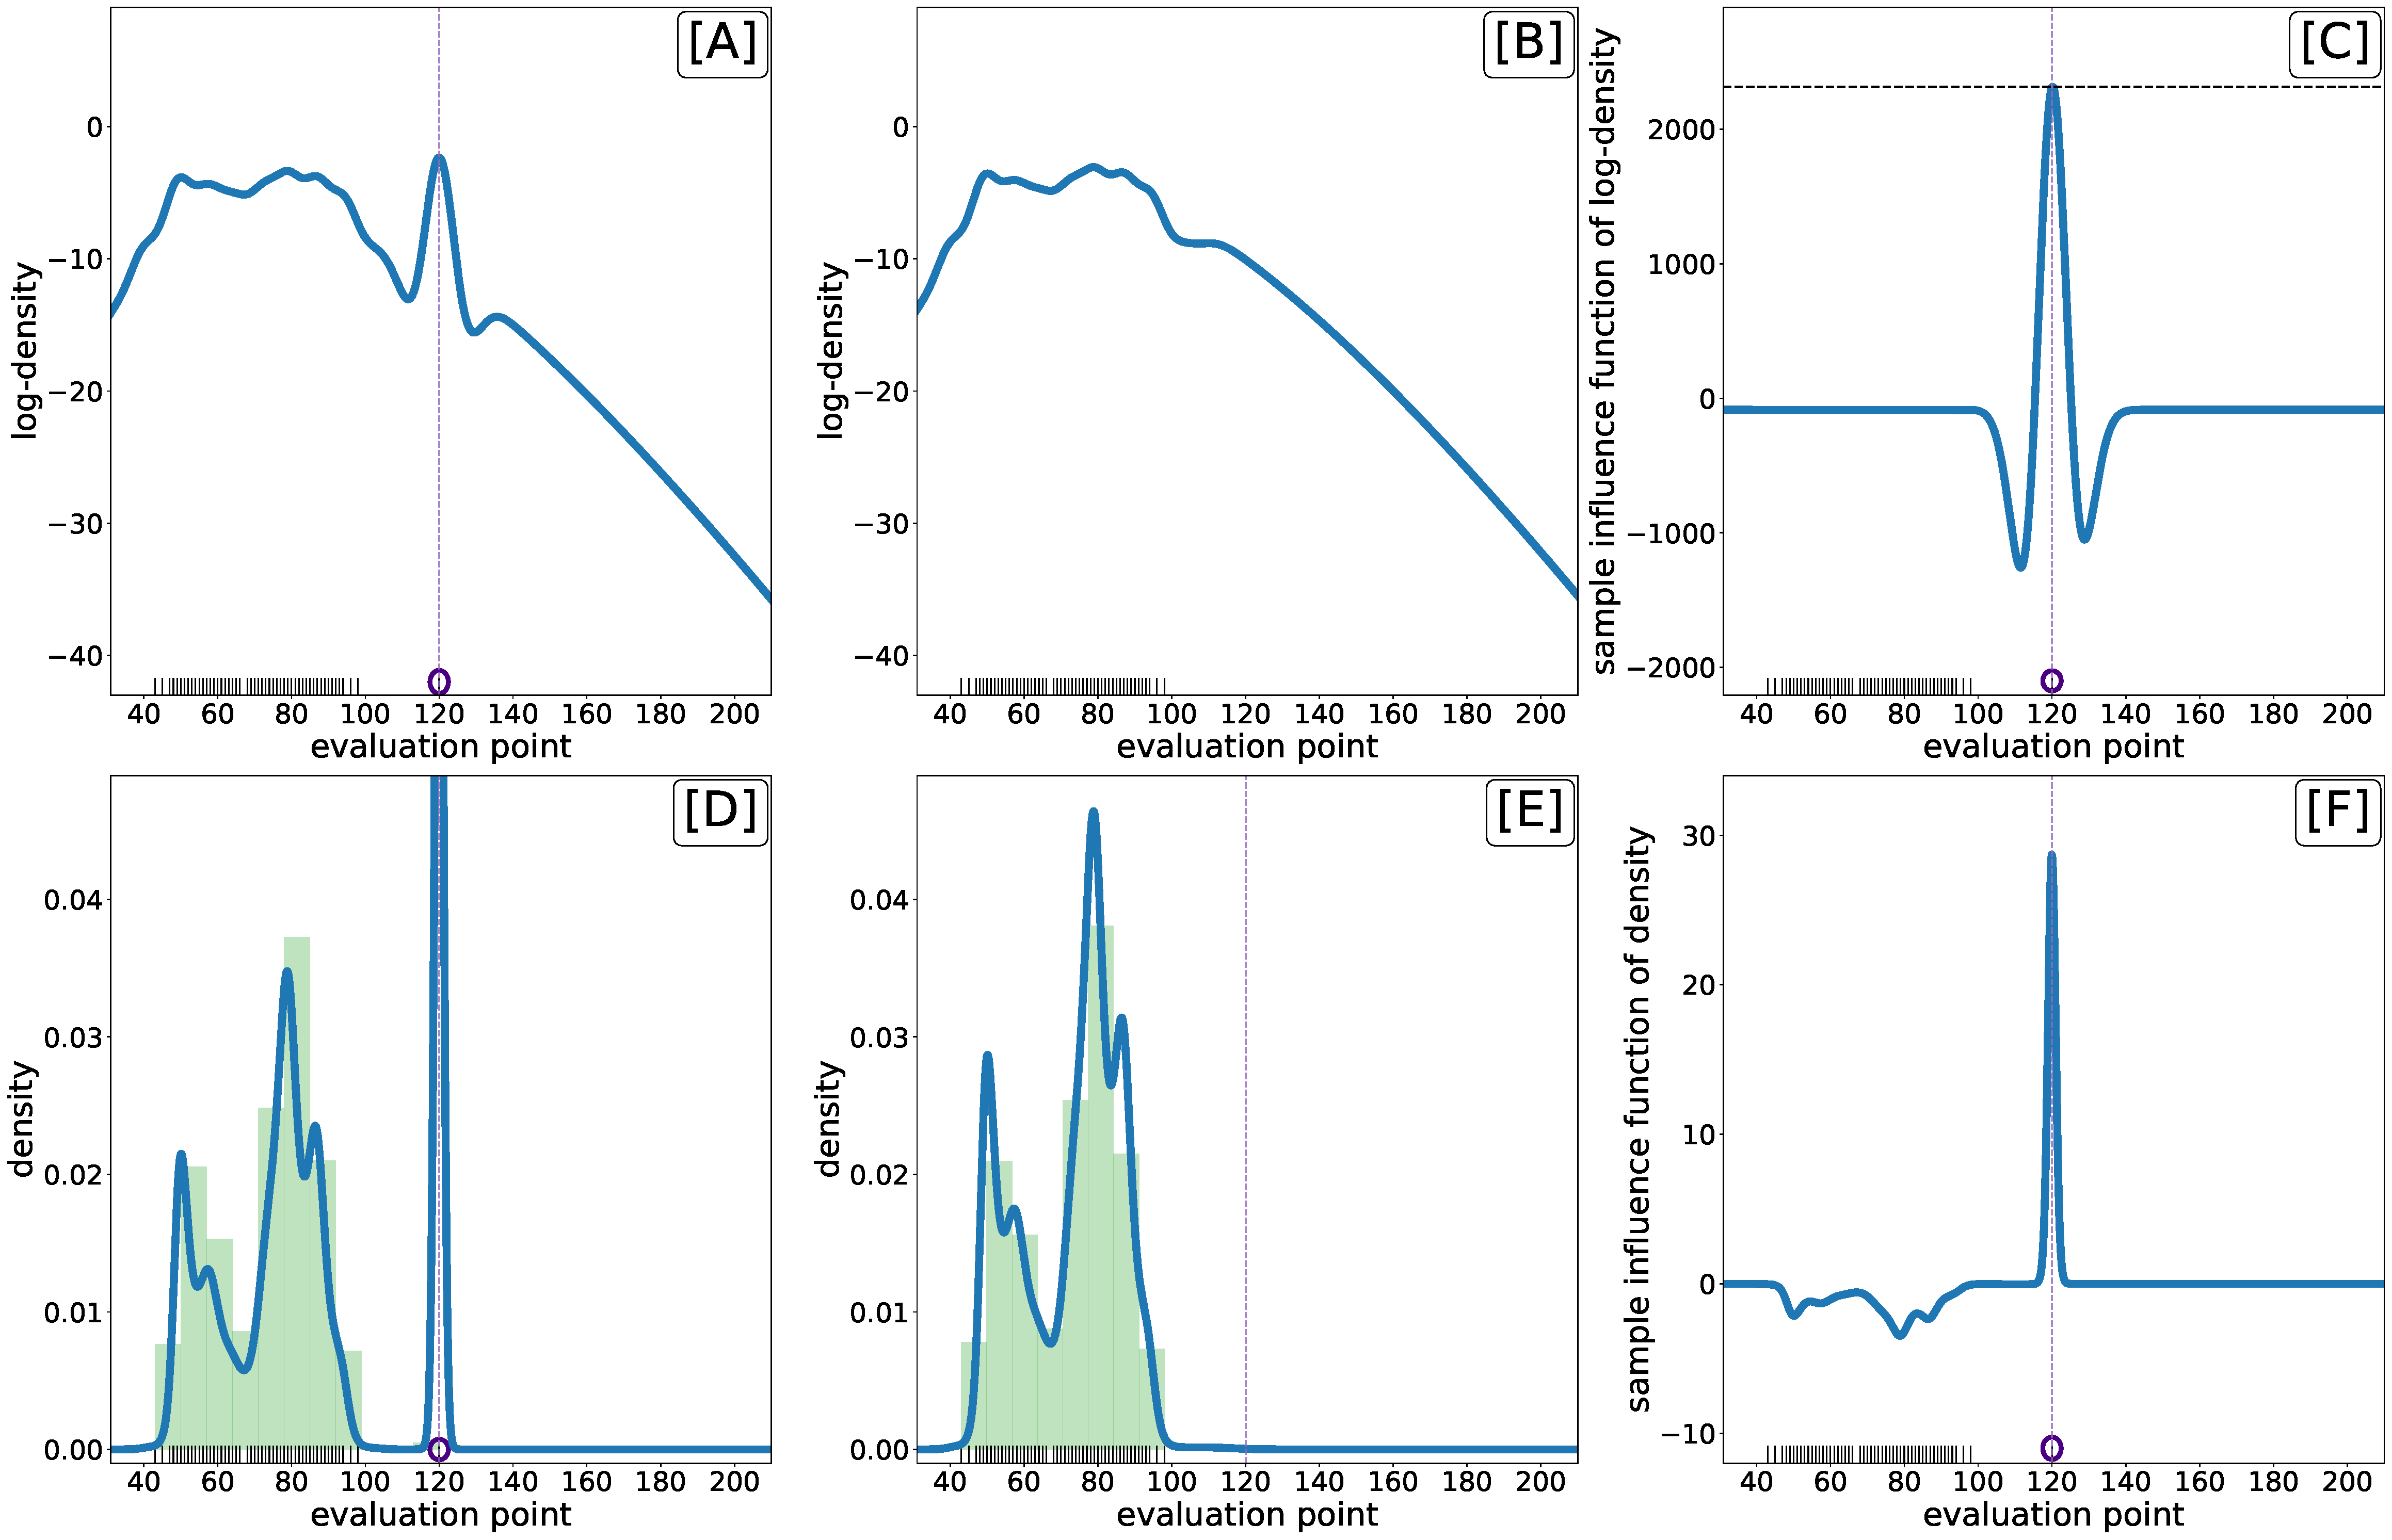
\includegraphics[width=\textwidth]{../plots/comparison-inffunden-inffunlogden-logdensity-density-contam-sm-logpenparam=-11.0-data=120.0-gamma-36.0-2.0.pdf}
	\caption{Fix $\rho = e^{-11}$. Panels [A] and [B] show the penalized SM log-density estimates with and without the additional observation $y = 120$, respectively. Panel [C] shows the sample influence function of the log-density estimator. Panels [D] and [E] show the penalized SM density estimates with and without the additional observation $y = 120$, respectively. Panel [F] shows the sample influence function of the density estimator. The rug plot indicates the location of data and the purple circle indicates the location of the observation $y=120$.}
	\label{fig-inffun-logdensity-vs-density-sm-y=120}
\end{figure}

\begin{figure}% [h!]
	\centering 
	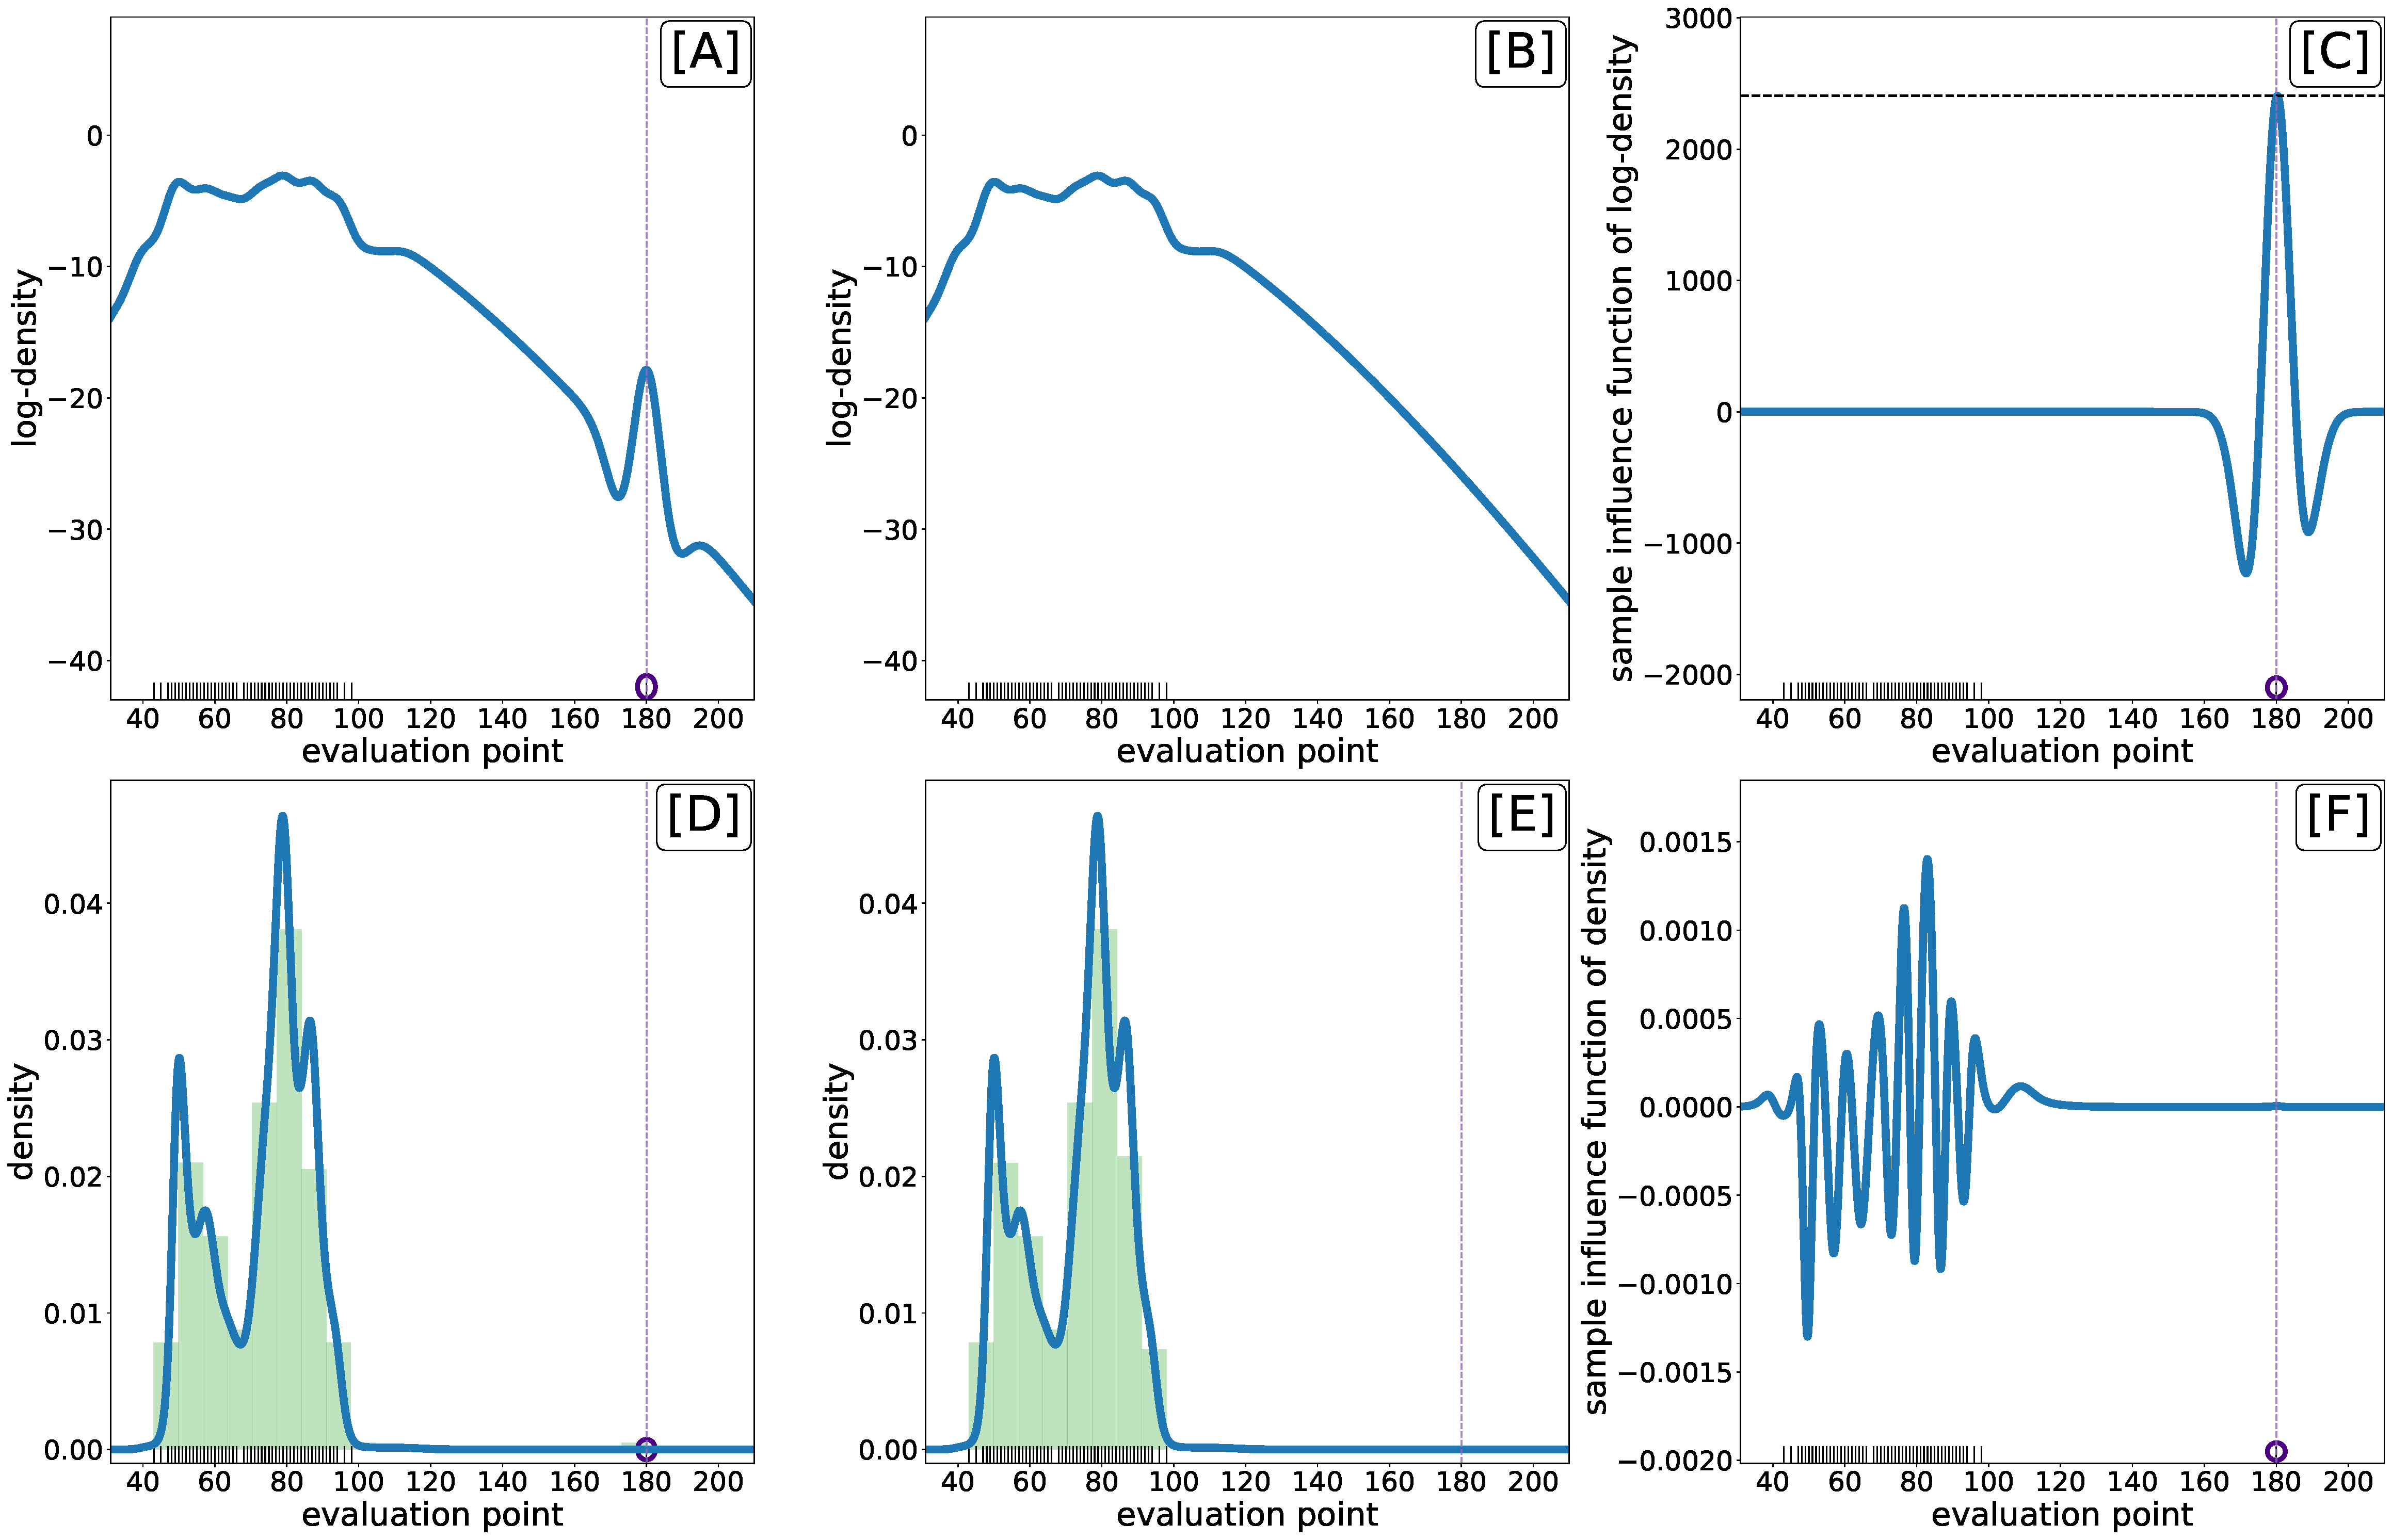
\includegraphics[width=\textwidth]{../plots/comparison-inffunden-inffunlogden-logdensity-density-contam-sm-logpenparam=-11.0-data=180.0-gamma-36.0-2.0.pdf}
	\caption{Fix $\rho = e^{-11}$. Panels [A] and [B] show the penalized SM log-density estimates with and without the additional observation $y = 180$, respectively. Panel [C] shows the sample influence function of the log-density estimator. Panels [D] and [E] show the penalized SM density estimates with and without the additional observation $y = 180$, respectively. Panel [F] shows the resulting sample influence function of the density estimator. The rug plot indicates the location of data and the purple circle indicates the location of the observation $y=180$.}
	\label{fig-inffun-logdensity-vs-density-sm-y=180}
\end{figure}

\begin{figure}% [h!]
	\centering 
	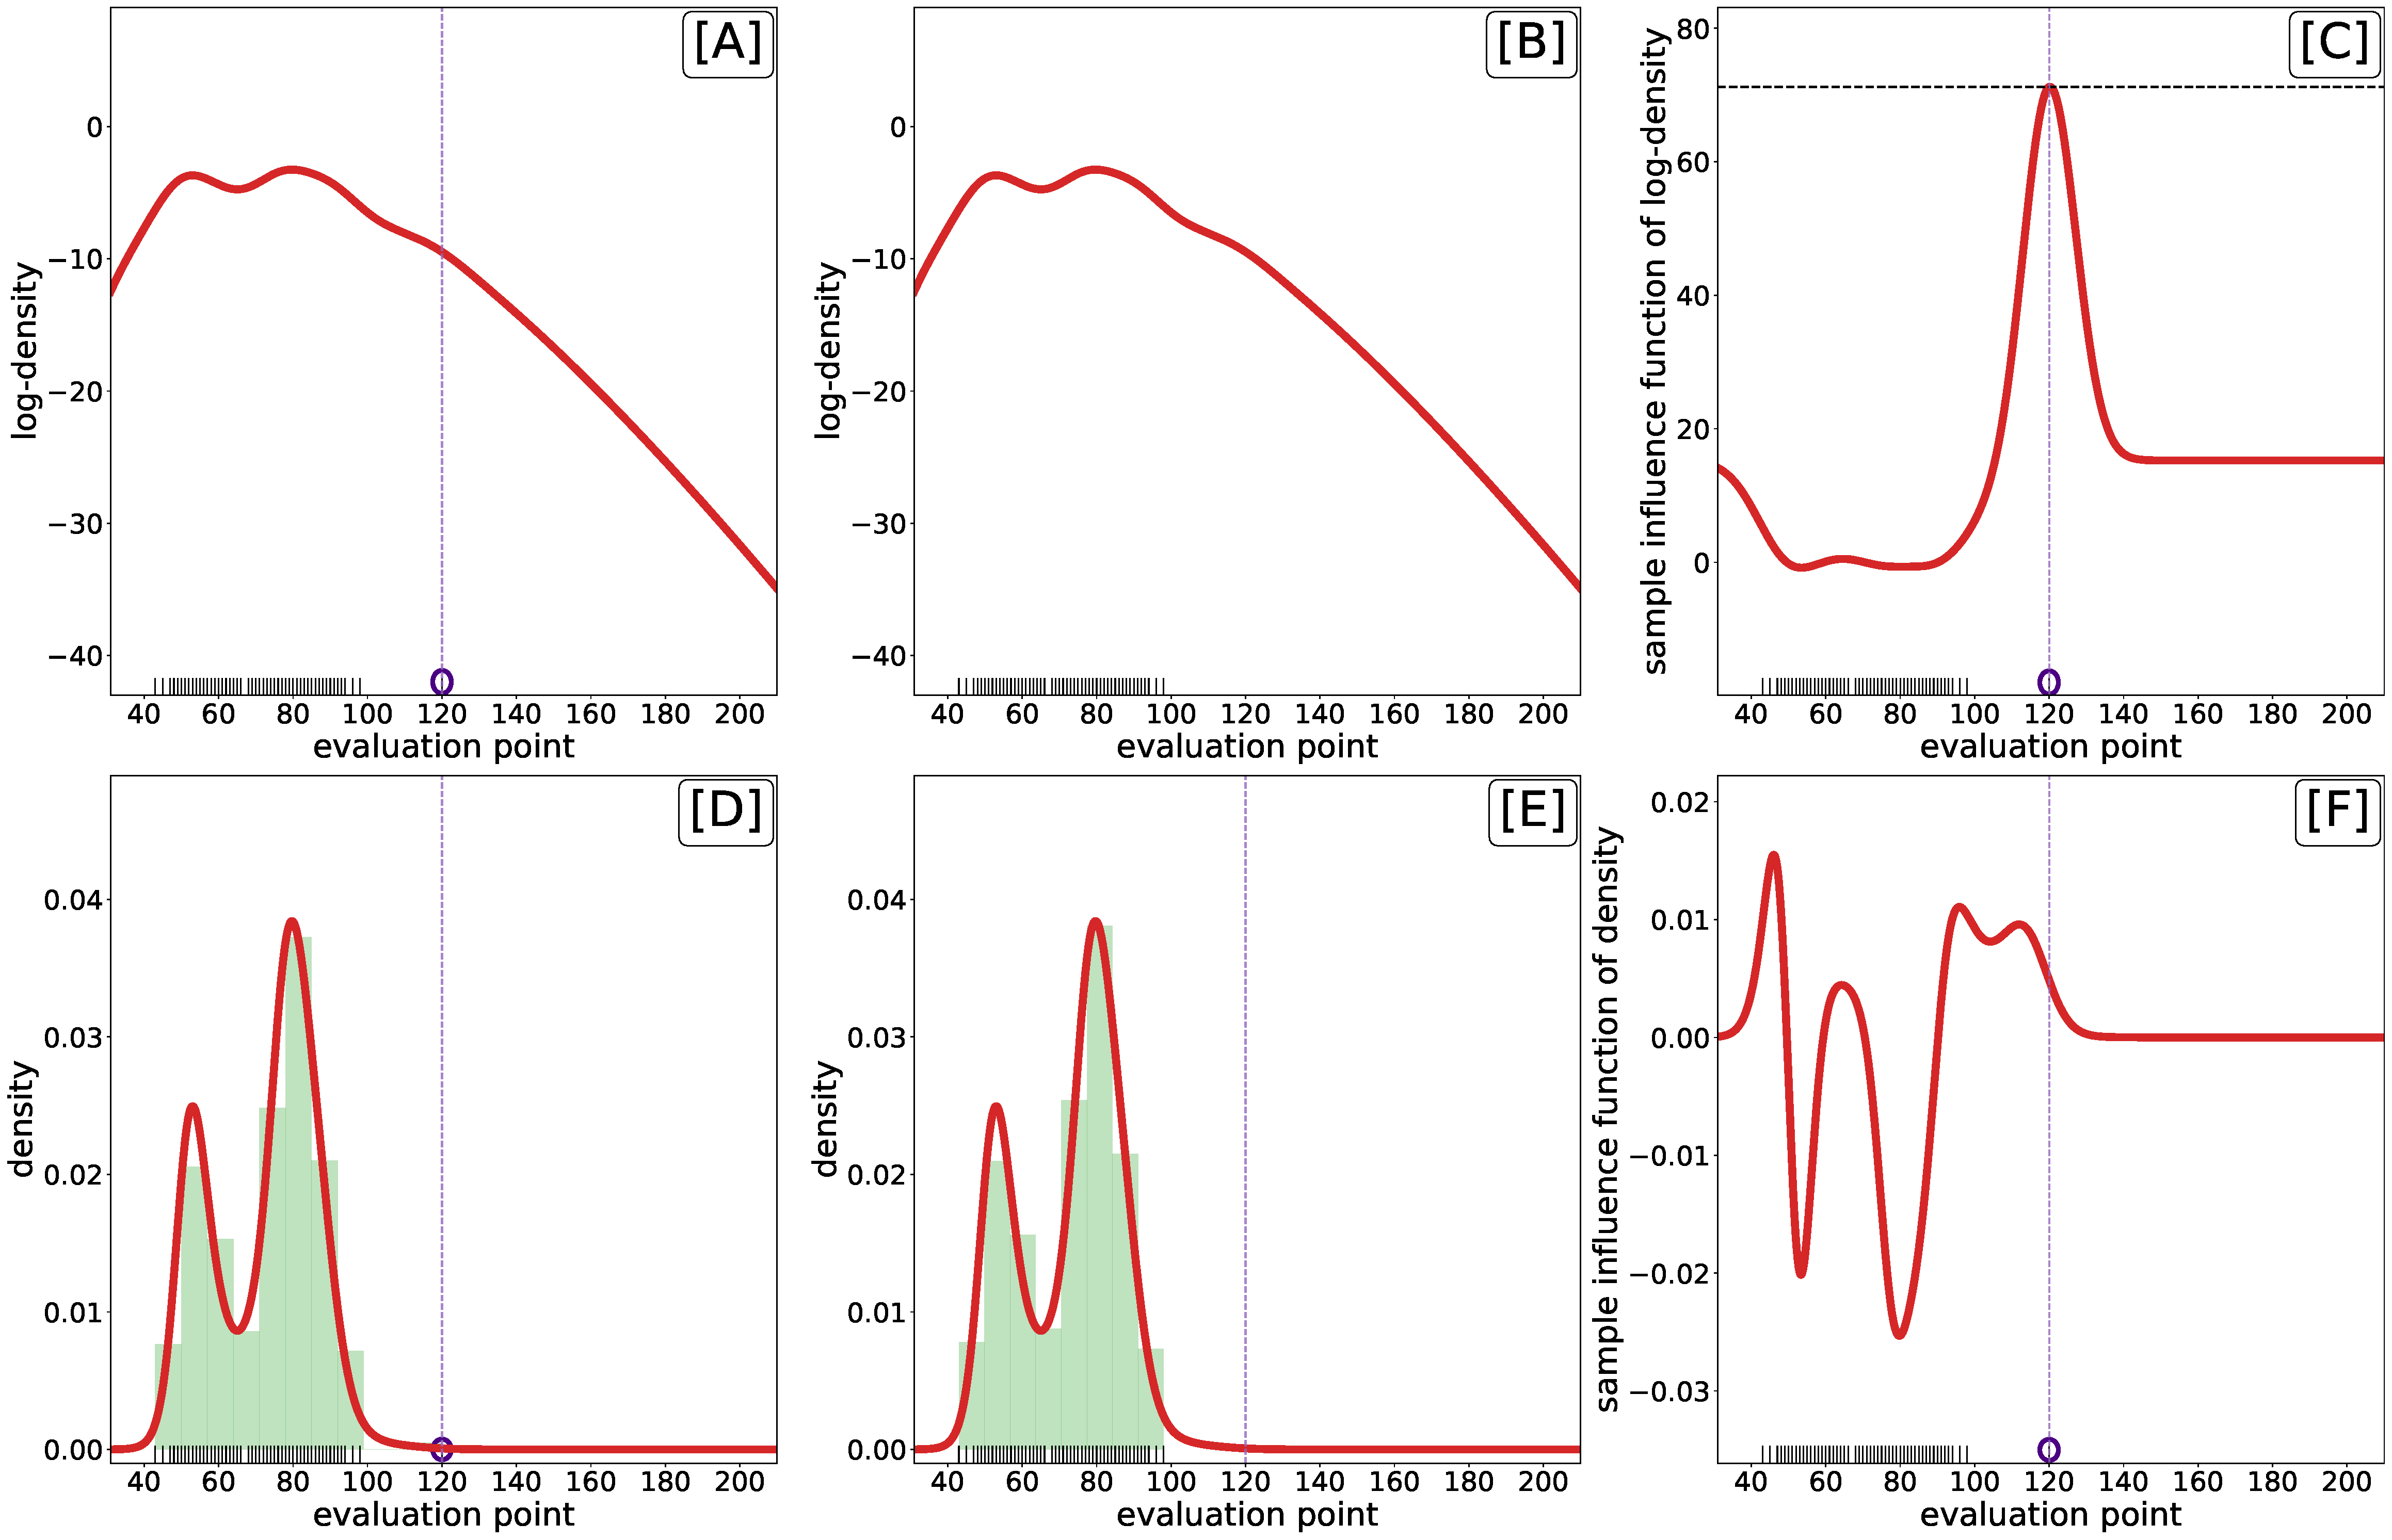
\includegraphics[width=\textwidth]{../plots/comparison-inffunden-inffunlogden-logdensity-density-contam-ml-logpenparam=-15.0-data=120.0-gamma-36.0-2.0.pdf}
	\caption{Fix $\lambda = e^{-15}$. Panels [A] and [B] show the penalized ML log-density estimates with and without the additional observation $y = 120$, respectively. Panel [C] shows the sample influence function of the log-density estimator. Panels [D] and [E] show the penalized SM density estimates with and without the additional observation $y = 120$, respectively. Panel [F] shows the resulting sample influence function of the density estimator. The rug plot indicates the location of data and the purple circle indicates the location of the observation $y=120$.}
	\label{fig-inffun-logdensity-vs-density-ml-y=120}
\end{figure}

\begin{figure}% [h!]
	\centering 
	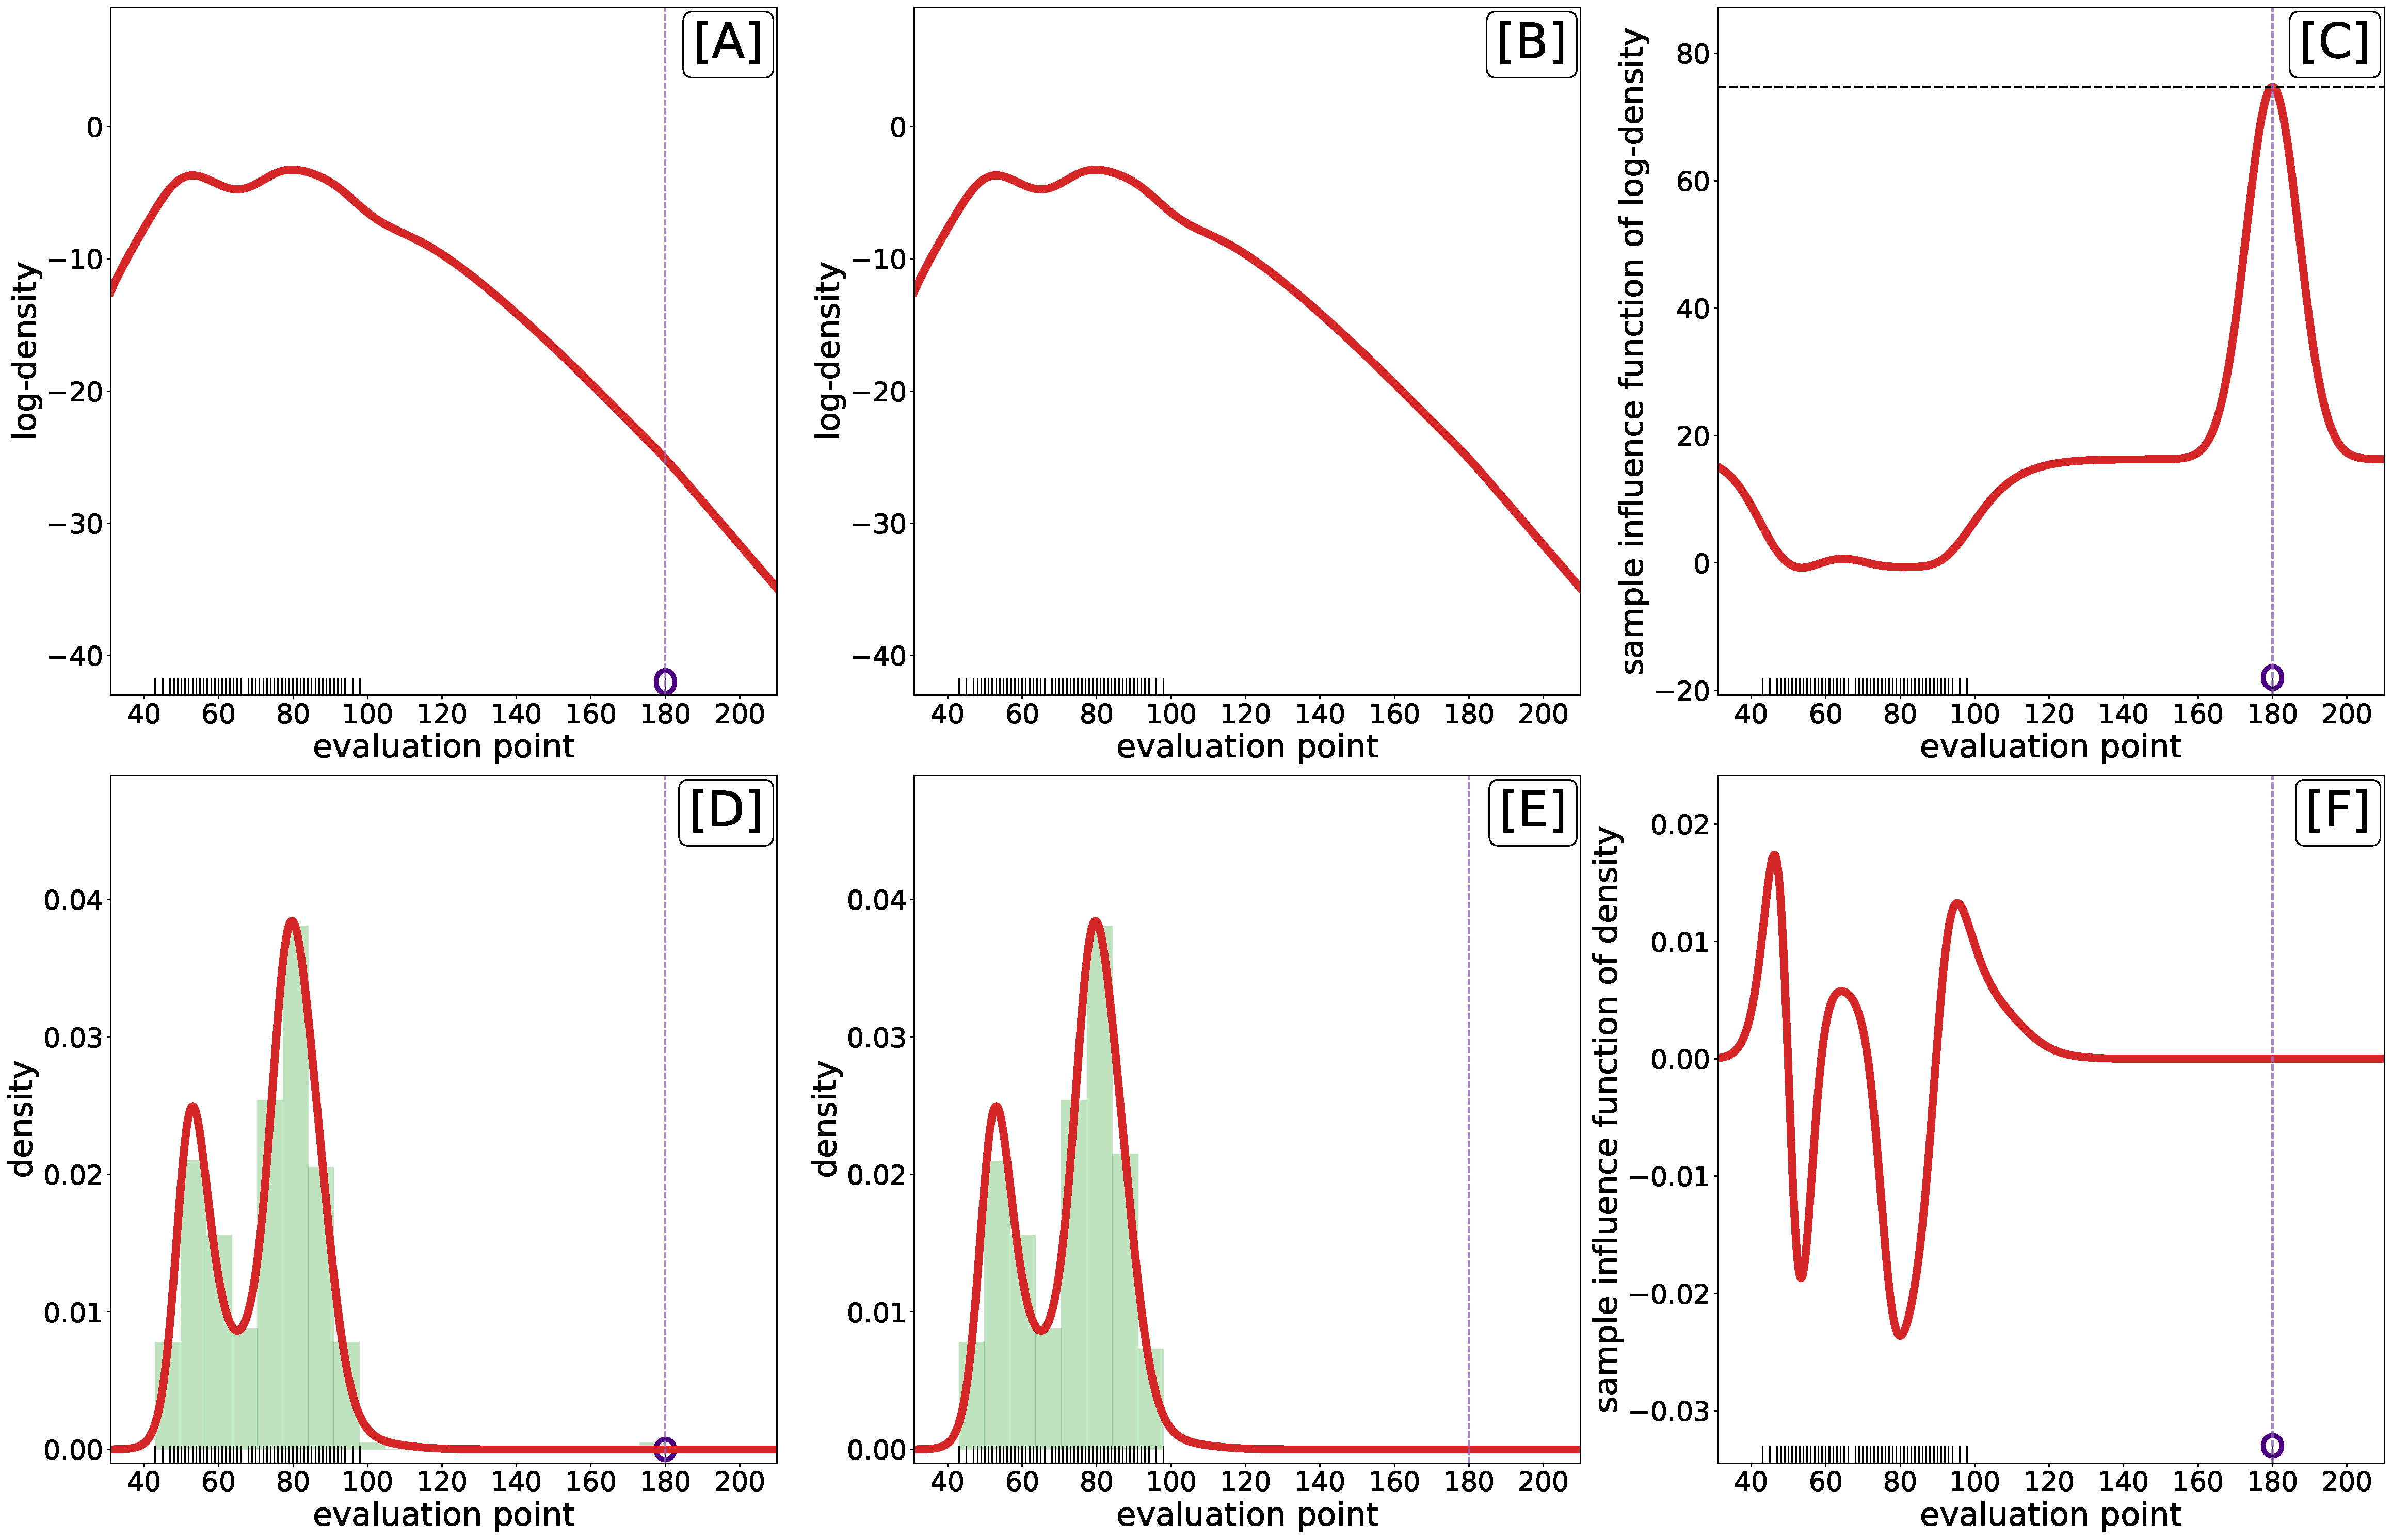
\includegraphics[width=\textwidth]{../plots/comparison-inffunden-inffunlogden-logdensity-density-contam-ml-logpenparam=-15.0-data=180.0-gamma-36.0-2.0.pdf}
	\caption{Fix $\lambda = e^{-15}$. Panels [A] and [B] show the penalized ML log-density estimates with and without the additional observation $y = 180$, respectively. Panel [C] shows the sample influence function of the log-density estimator. Panels [D] and [E] show the penalized SM density estimates with and without the additional observation $y = 180$, respectively. Panel [F] shows the resulting sample influence function of the density estimator. The rug plot indicates the location of data and the purple circle indicates the location of the observation $y=180$.}
	\label{fig-inffun-logdensity-vs-density-ml-y=180}
\end{figure}

Analytically, note that 
\begin{align*}
	& \, S_{\rho} \parens{ \parens{1 - \varepsilon_0} F_n + \varepsilon_0 \delta_y } \parens{x} - S_{\rho} \parens{F_n} \parens{x} \\ 
	= & \, \bracks[\big]{ \cancel{\log \mu \parens{x}} + f_{\SM, \parens{1 - \varepsilon_0} F_n + \varepsilon_0 \delta_y}^{\parens{\rho}} \parens{x} - A \parens{f_{\SM, \parens{1 - \varepsilon_0} F_n + \varepsilon_0 \delta_y}^{\parens{\rho}} } } \\ 
	& \qquad \quad - \bracks[\big]{ \cancel{\log \mu \parens{x}} + f_{\SM, F_n}^{\parens{\rho}} \parens{x} - A \parens{f_{\SM, F_n}^{\parens{\rho}} } } \\
	= & \, \bracks[\big]{ f_{\SM, \parens{1 - \varepsilon_0} F_n + \varepsilon_0 \delta_y}^{\parens{\rho}} \parens{x} - A \parens{f_{\SM, \parens{1 - \varepsilon_0} F_n + \varepsilon_0 \delta_y}^{\parens{\rho}} } } - \bracks[\big]{ f_{\SM, F_n}^{\parens{\rho}} \parens{x} - A \parens{f_{\SM, F_n}^{\parens{\rho}} } }, 
\end{align*}
from which we see $\mathrm{SIF}_{x, \varepsilon_0} \parens{S_{\rho}, F, y}$ does \textit{not} depend on $\mu \parens{x}$, but only on the natural parameter part. If we work with $\mathrm{SIF}_{x, \varepsilon_0} \parens{\widetilde{S}_{\rho}, F, y}$, however, we have 
\begin{align*}
	& \, \widetilde{S}_{\rho} \parens{ \parens{1 - \varepsilon_0} F_n + \varepsilon_0 \delta_y } \parens{x} - \widetilde{S}_{\rho} \parens{F_n} \parens{x} \\ 
	= & \, \mu \parens{x} \bracks[\Big]{\exp \parens[\big]{f_{\SM, \parens{1 - \varepsilon_0} F_n + \varepsilon_0 \delta_y}^{\parens{\rho}} \parens{x} - A \parens{f_{ \SM, \parens{1 - \varepsilon_0} F_n + \varepsilon_0 \delta_y}^{\parens{\rho}}}} - \exp \parens[\big]{f_{\SM, F_n}^{\parens{\rho}} \parens{x} - A \parens{f_{\SM, F_n }^{\parens{\rho}}}} }, 
\end{align*}
and we cannot get rid of $\mu \parens{x}$ in the front. The resulting $\mathrm{SIF}_{x, \varepsilon_0} \parens{\widetilde{S}_{\rho}, F, y}$ inevitably depends on $\mu \parens{x}$. By a similar approach as above, we can also see $\mathrm{SIF}_{x, \varepsilon_0} \parens{T_{\lambda}, F, y}$ does \textit{not} depend on $\mu \parens{x}$ but $\mathrm{SIF}_{x, \varepsilon_0} \parens{\widetilde{T}_{\lambda}, F, y}$ does. 

Thus, from both numerical examples and analytic analysis, we see the sample influence function of the \emph{log-}density estimator is the better choice than that of the density estimator. Hence, we will only consider the former in the sequel. 


\subsection{Comparison of the Sensitivities}\label{subsection-main-comparison-sensitivity}

Our goal of this section is to compare the sensitivities of the penalized ML and SM density estimators in $\calQ_{\ker}$. 

Let us still fix $\rho = e^{-11}$ and $y = 120$, and return to the first row of Figure \ref{fig-inffun-logdensity-vs-density-sm-y=120} where we show $S_{\rho} \parens{\parens{1 - \varepsilon_0} F_n + \varepsilon_0 \delta_y}$, $S_{\rho} \parens{F_n}$, and the resulting sample influence function evaluated at different points. It is apparent that $y = 120$ has different effects on $S_{\rho}$ at different evaluation points. The overall influence of $y$ on $S_{\rho}$, $\widehat{M}_{\varepsilon_0} \parens{S_{\rho}, F_n, y}$, is approximately equal to 2315.48, which is achieved roughly at 120. 

Let us still fix $\rho = e^{-11}$ but vary $y$. The left panel in Figure \ref{fig-SM-overall} shows the overall influence of $y$ on $S_{\rho}$ against different choices of $y$. It is obvious that different locations of $y$ have different overall influences on $S_{\rho}$. When $y$ is below 40 or above 100 (low-density region), it has a larger overall influence on $S_{\rho}$; and when $y$ is between 40 and 100 (high-density region), it has a smaller overall influence. 

\begin{figure}[h]
	\centering
	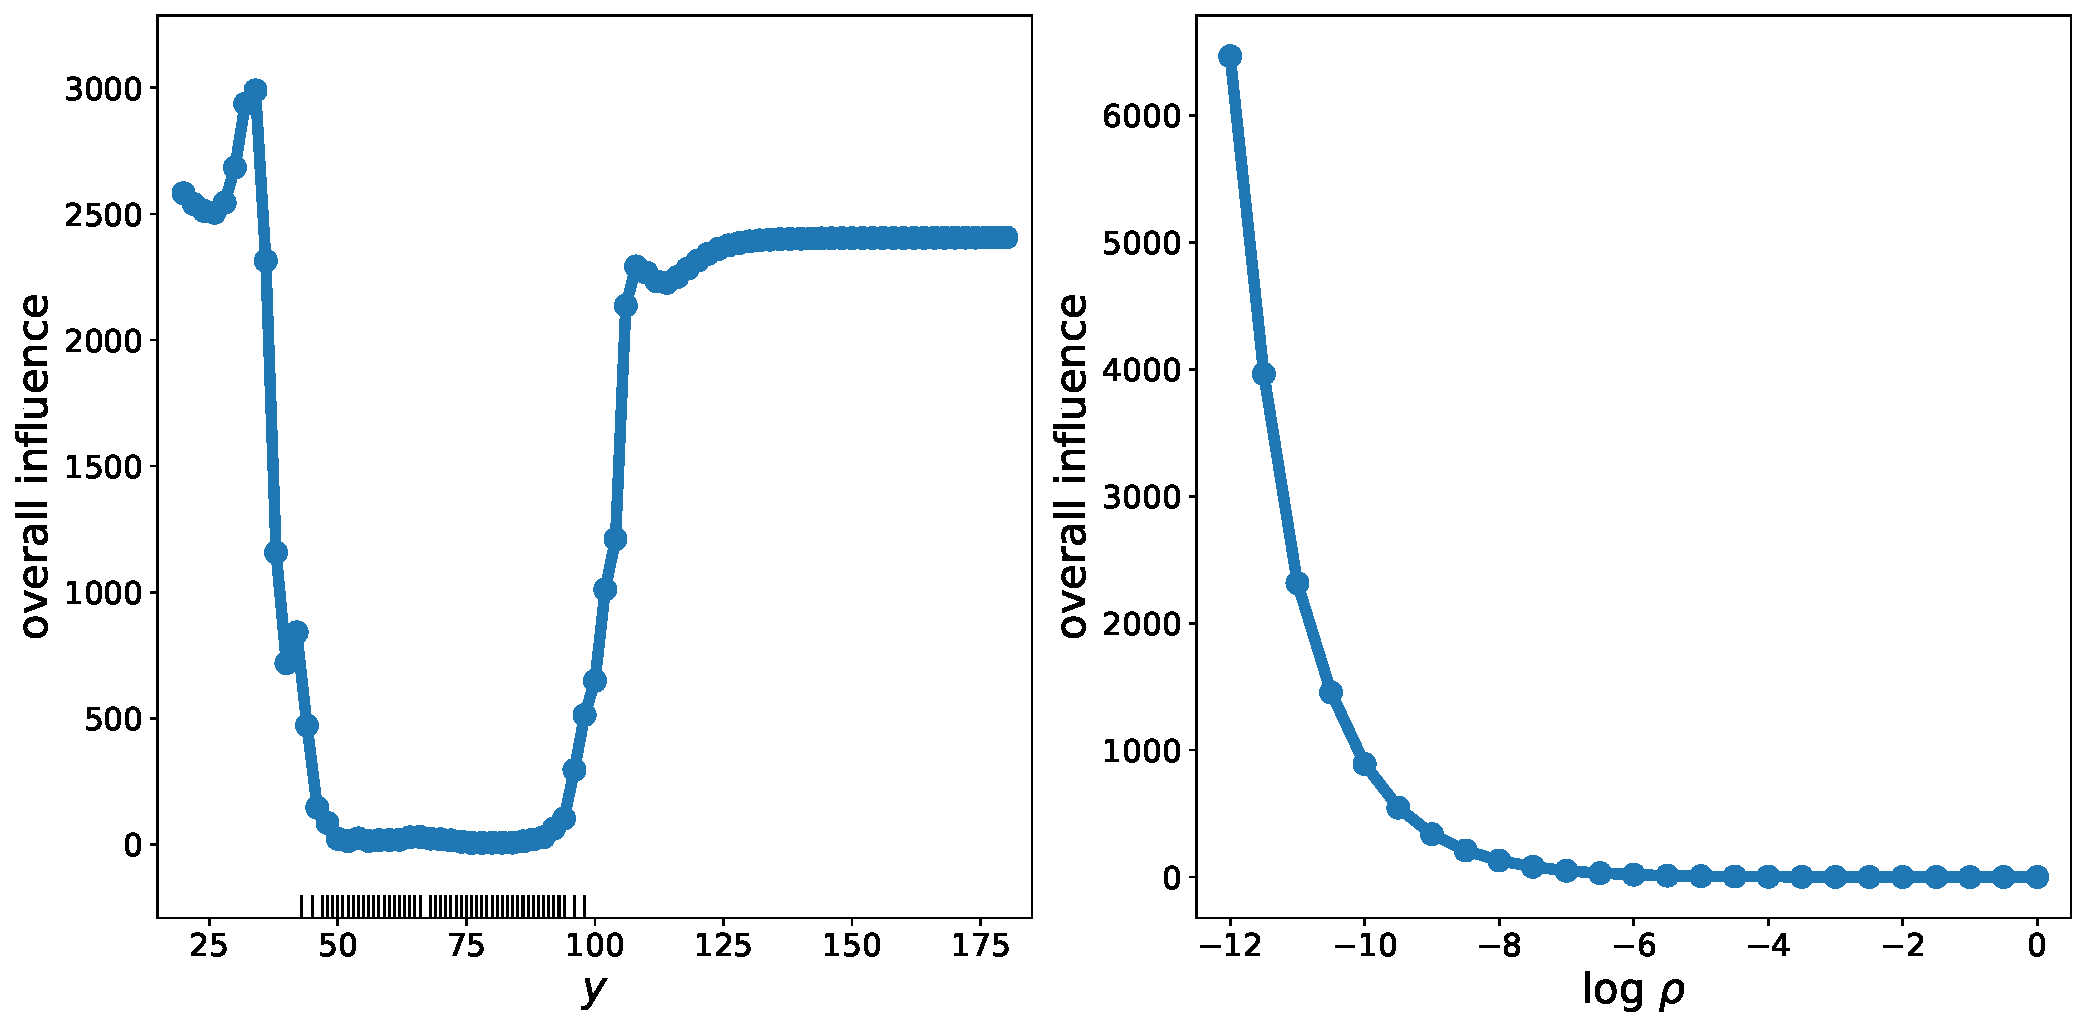
\includegraphics[width=\textwidth]{../plots/waiting-SM-overall-empirical-influence-log-density-estimates-baseden=Gamma-36-2-gridpoints=1-202-1.pdf}
	\caption{Left panel shows the overall influence versus different choices of $y$, where we fix $\rho = e^{-11}$ and the rug plot indicate the location of the \texttt{waiting} data. Right panel shows the overall influence against different choices of $\rho$ (shown in log scale), where we fix $y = 120$.}
	\label{fig-SM-overall}
\end{figure}

Now, fix $y = 120$ but vary the values of $\rho$. The right panel in Figure \ref{fig-SM-overall} shows the overall influence of $y = 120$ on $S_{\rho}$ versus different choices of $\rho$. It is obvious that the overall influence of $y$ keeps increasing as the value of $\rho$ keeps decreasing. 

Thus, both the location of $y$ and the value of $\rho$ impact the overall influence on log-density estimators. To exhibit the sensitivity of the penalized SM log-density estimators subject to these two factors, a natural idea is to plot the heat map of the overall influence against them, which is shown in Figure \ref{fig-SM-overall-influence-y-rho}. However, recall our ultimate goal is to compare the sensitivities of both penalized ML and SM density estimators, and their respective penalty parameters, $\lambda$ and $\rho$, are on different scales. Thus, plotting the penalty parameter on the horizontal axis is not conducive to comparison. Instead, we plot the RKHS norm of natural parameter under $F_n$, i.e., $\norm{f_{\ML, F_n}^{\parens{\lambda}}}_{\calH}$ and $\norm{f_{\SM, F_n}^{\parens{\rho}}}_{\calH}$, on the horizontal axis. The smaller the penalty parameter is, the larger the RKHS norm of the natural parameter is. 

\begin{figure}[h]
	\centering
	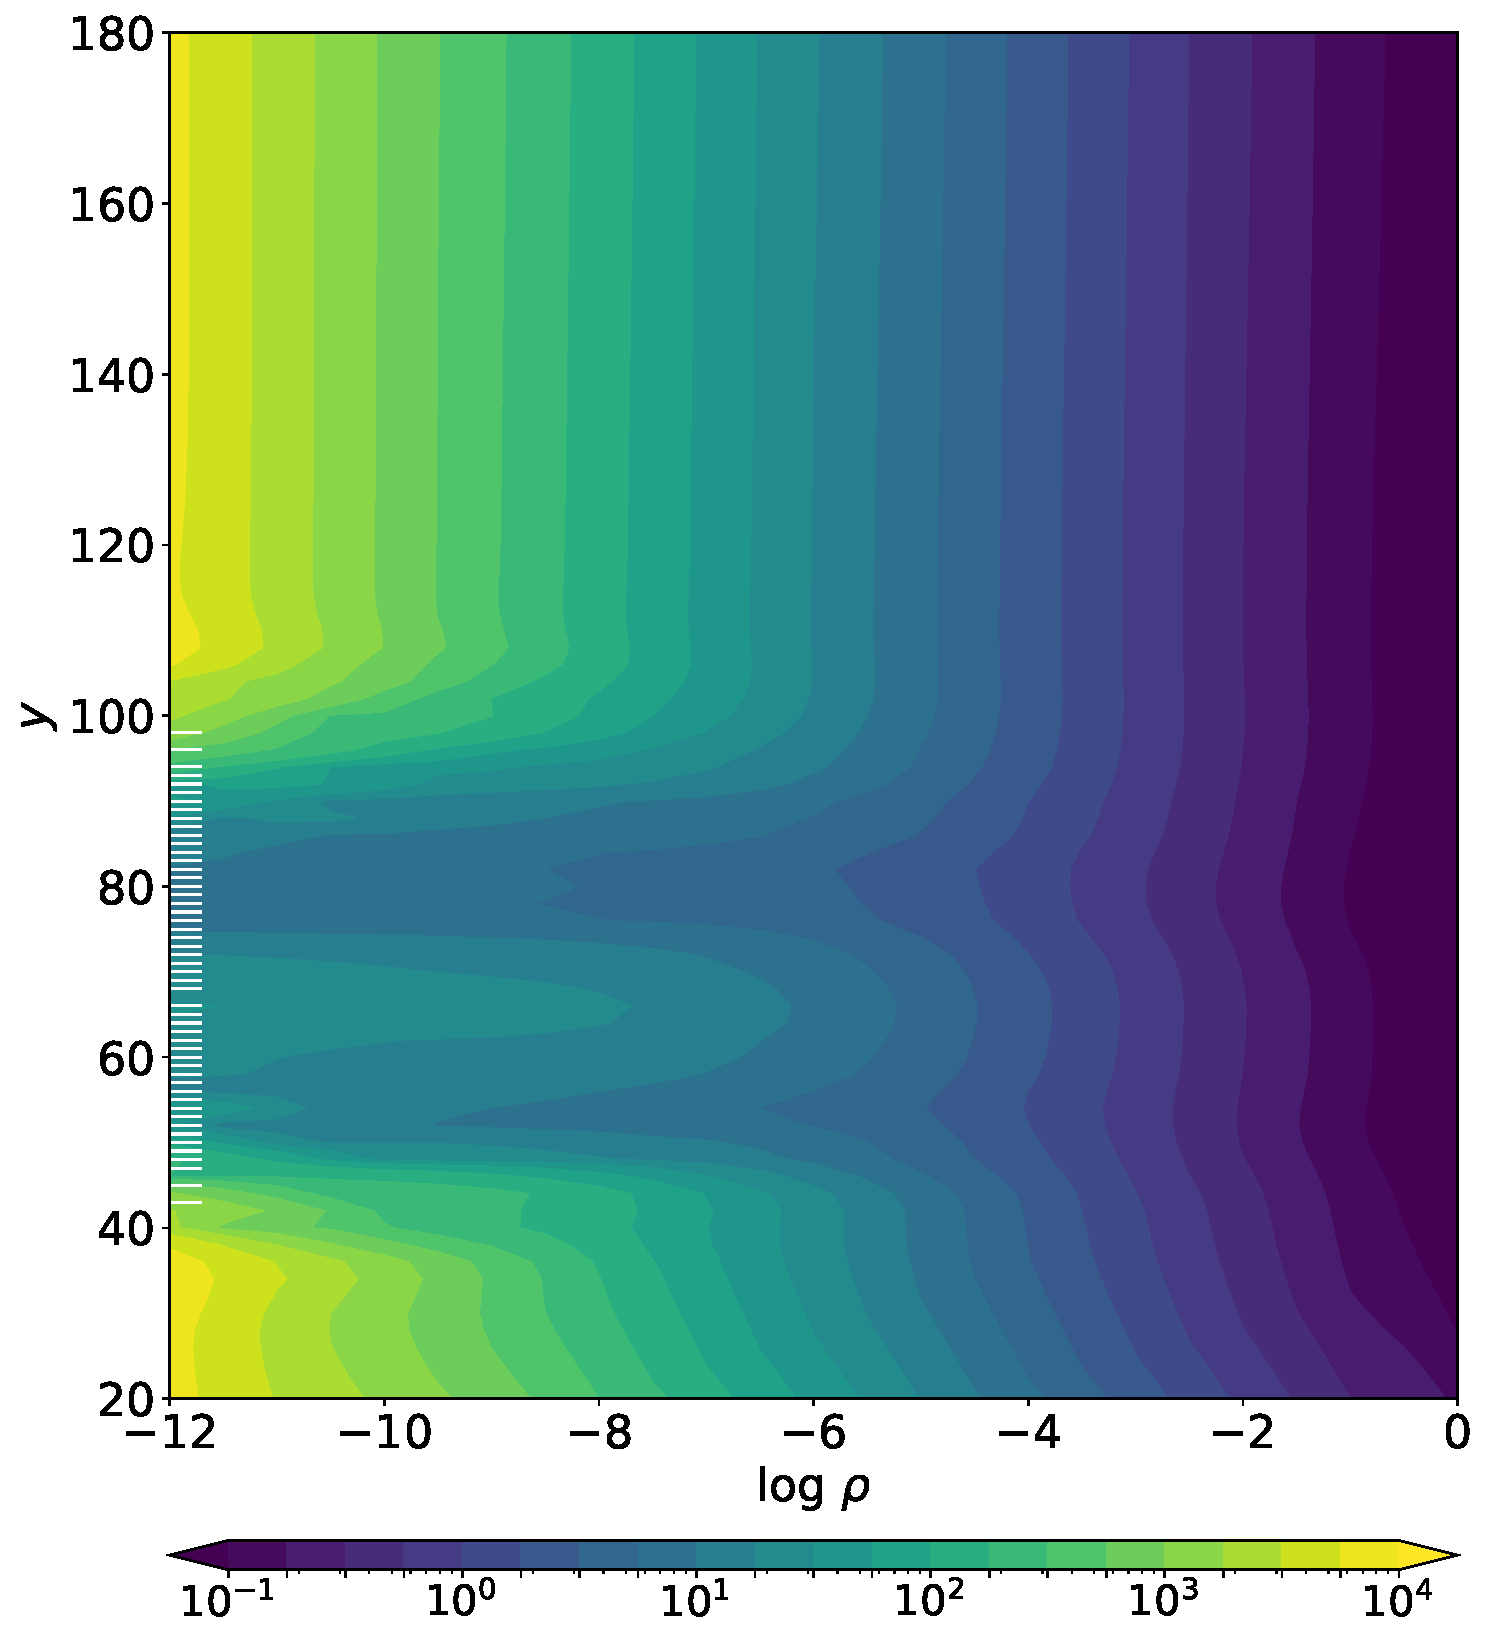
\includegraphics[width=0.6\textwidth]{../plots/PenSMFin-PenML-geyser-waiting-logdensity-empIF-supnorm-penaltyparameter-heatmap-bw=5.0-Gamma-36-2-gridpoints=1-202-1-logscale.pdf}
	\caption{Heat map of the overall influence on the penalized SM log-density estimates against $y$ and $\rho$ (shown in log scale). White rugs indicate locations of the \texttt{waiting} data.} 
	\label{fig-SM-overall-influence-y-rho}
\end{figure}

\begin{figure}[h!]
	\centering
	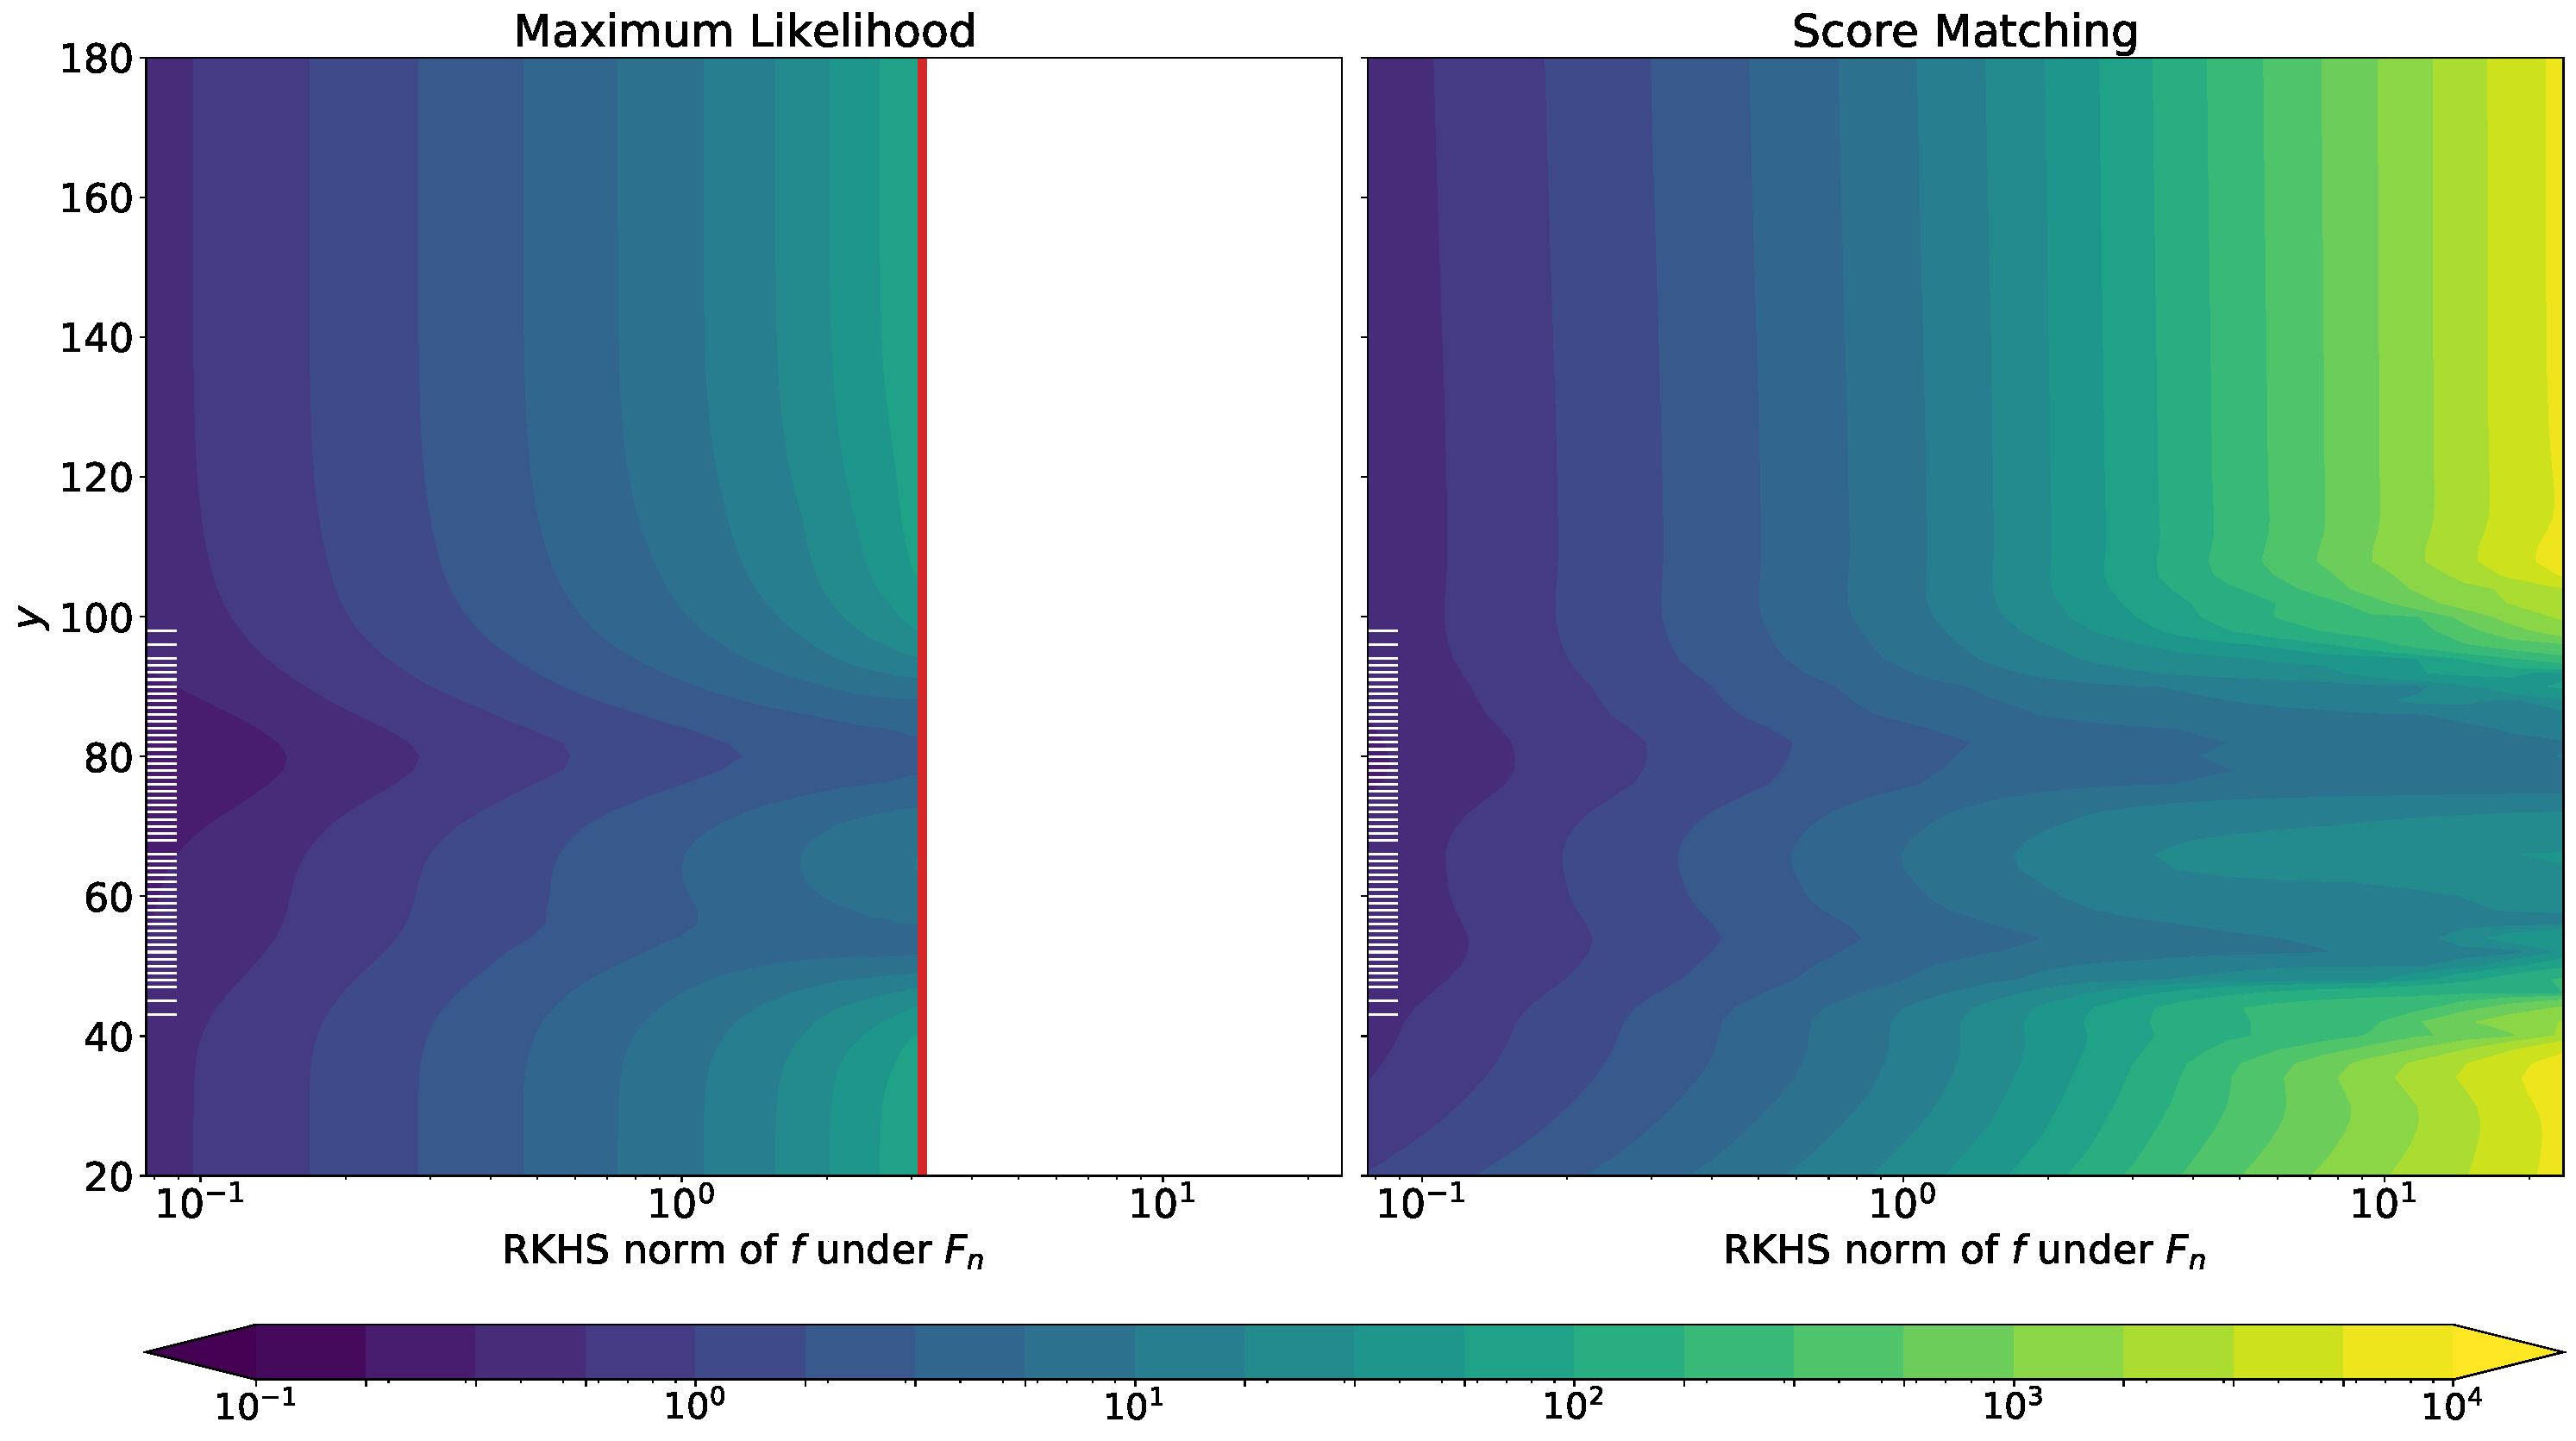
\includegraphics[width=\textwidth]{../plots/PenSMFin-PenML-geyser-waiting-logdensity-empIF-supnorm-natparamnorm-heatmap-bw=5.0-Gamma-36-2-gridpoints=1-202-1-logscale.pdf}
	\caption{Heat maps of the overall influence on penalized ML (left) and SM (right) log-density estimates against $y$ and the RKHS norm of the natural parameter under $F_n$ (shown in log scale). Red vertical line in left panel indicates the case $\lambda = 0$. White rugs indicate locations of the \texttt{waiting} data.}
	\label{fig-SM-overall-influence-y-norm}
\end{figure}

The resulting heat maps for the penalized ML and SM density estimates are shown in Figure \ref{fig-SM-overall-influence-y-norm}, where we choose $y = 20, 22, \cdots, 180$, $\lambda = 0, e^{-15}, e^{-14.5}, \cdots, e^{0.5}, e^{1}$, and $\rho = e^{-12}, e^{-11.5}, \cdots, e^{0}$. If we look at each panel individually, findings are consistent as before: with a fixed value of the penalty parameter, $y$ in the low-density region has a larger overall influence on log-density estimates than that in the high-density region; with a fixed $y$, a larger RKHS norm of the natural parameter (corresponding to a smaller penalty parameter value) implies a larger overall influence of $y$. In particular, if we fix a $y$ value, say $y_0$, the maximal possible overall influence of $y_0$ on the penalized ML density estimates for all values of $\lambda \ge 0$ is the intersection of $y = y_0$ and the red vertical line, which corresponds to the overall influence of $y_0$ on the unpenalized ML density estimate (i.e., $\lambda = 0$). 

If we compare two panels in Figure \ref{fig-SM-overall-influence-y-norm}, we observe that, for each choice of $y$, as we decrease the values of penalty parameters so that the RKHS norm of $f$ under $F_n$ keeps increasing, the overall influences on the penalized ML density estimates stop increasing at the red vertical line, but that on the penalized SM density estimates can continue increasing. In other words, for each choice of $y$, the overall influences on the penalized SM log-density estimates with sufficiently small values of $\rho > 0$ are larger than the overall influence on the \emph{unpenalized} ML log-density estimate, implying that, when there is a small amount of penalization, the penalized SM density estimator is more sensitive to an additional observation (not only to the isolated observation) than the unpenalized and penalized ML density estimator. Additional numerical examples also confirm our observations here. 


\section{The Sensitivity of $K$-fold Cross-validated Penalized Score Matching Density Estimator}\label{section-sensitivity-cv-penalized-sm-density-estimator}

$K$-fold cross-validation (CV) is perhaps the most popular method to choose the penalty parameter in practice. In this section, we are going to investigate whether the $K$-fold cross-validated penalized SM density estimator is sensitive to the presence of an additional observation or not. The procedure of computing the overall influence of $y$ on the $K$-fold cross-validated penalized SM density estimator is shown in Algorithm \ref{algo-sensitivity-cv-sm-density-estimator}. 

\begin{algorithm}
\caption{Computation of the overall influence of $K$-fold cross-validated penalized SM density estimator}\label{algo-sensitivity-cv-sm-density-estimator}
\begin{algorithmic}[1]
\Statex \algorithmicrequire 
\begin{itemize}\setlength\itemsep{0em}
	\item $X_1, \cdots, X_n$, data; 
	\item $y \in \calX$, contaminant; 
	\item $K$, the number of folds in CV; 
	\item $\sets{\rho_j}_{j=1}^{M}$, a list of penalty parameter candidates; 
	\item $\widetilde{\calH}$, the finite-dimensional approximating subspace over which we minimize the penalized NLL loss functional; 
	\item $\sets{x_{\ell}}_{\ell=1}^L \subset \calX$, a set of dense evaluation points in $\calX$. 
\end{itemize}

\vspace{5pt}

\State Compute the best density estimate using $X_1, \cdots, X_n$ with the penalty parameter selected by CV; denote the resulting log-density estimate by $S_{\mathrm{CV}} \parens{F_n}$; 
\State Compute the best density estimate using $X_1, \cdots, X_n$ and $y$ with the penalty parameter selected by CV; denoted the resulting log-density estimate by $S_{\mathrm{CV}} \parens{F_{n+1}}$; 
\State Compute 
\begin{align*}
	\mathrm{SIF}_{x_{\ell}, \varepsilon_0} \parens{S_{\mathrm{CV}}, F_n, y} := \parens[\Big]{S_{\mathrm{CV}} \parens{F_{n+1}} \parens{x_\ell} - S_{\mathrm{CV}} \parens{F_{n}} \parens{x_\ell}} \times \parens{n+1}, 
\end{align*}
for all $\ell = 1, \cdots, L$; 
\State \textbf{return} $\max_{\ell=1,\cdots,L} \abs[\big]{\mathrm{SIF}_{x_{\ell}, \varepsilon_0} \parens{S_{\mathrm{CV}}, F_n, y}}$. 
\end{algorithmic}
\end{algorithm}

We still use the \texttt{waiting} variable in the Old Faithful Geyser dataset and choose the number of folds to be $K = 3, 5, 10$. For each value of $K$, we replicate the procedures outlined in Algorithm \ref{algo-sensitivity-cv-sm-density-estimator} for 30 times. The additional observations $y$ we choose are the same as those in the preceding section, $y = 20, 22, \cdots, 180$. Figure \ref{fig-sensitivity-cv-sm-density-estimator} shows the results. 

\begin{figure}[t]
	\centering
	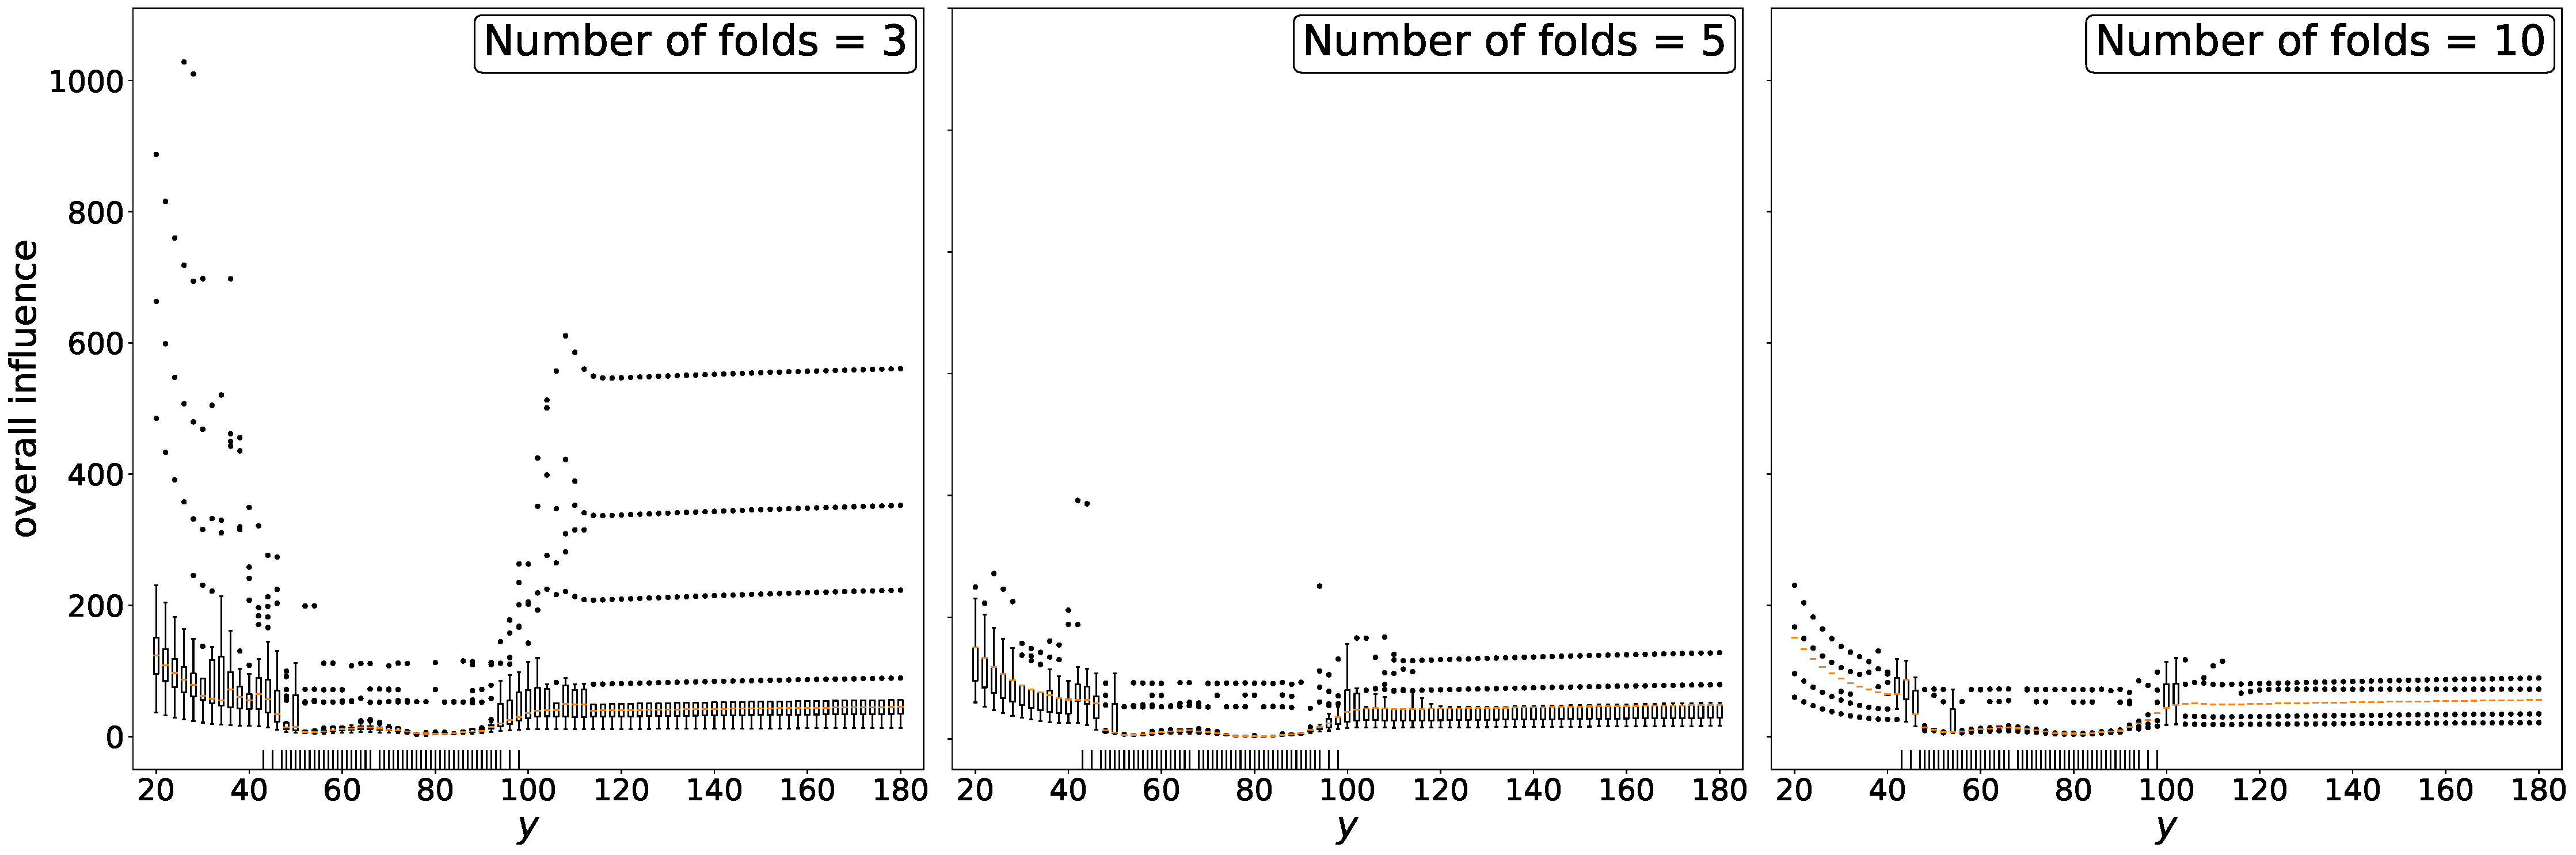
\includegraphics[width=\textwidth]{../plots/PenSMFin-geyser-waiting-overall-emp-influence-y-baseden=Gamma-36.0-2.0-gridpoints=1-202-1-cross-validation.pdf}
	\caption{Overall influence of $y$ on the $K$-fold cross-validated penalized SM density estimates against the values of $y$. We choose $K=3$ (left panel), 5 (middle panel), and 10 (right panel). In each panel, for each choice of $y$, we plot a boxplot of the overall influences of that particular $y$ value on $S_{\rho} \parens{F_n}$ obtained from 30 replications. }
	\label{fig-sensitivity-cv-sm-density-estimator}
\end{figure}

For each number of folds, similar to our earlier observations, when $y$ is in the high-density region (between 40 and 100), the overall influences of $y$ on cross-validated penalized SM density estimates tend to be small; and when $y$ is in the low-density region ($<40$ or $>100$), the overall influences of $y$ tend to be much larger. 

In addition, we see as the number of folds increases, the cross-validated penalized SM log-density estimates become less sensitive in general. %, which is mainly because, as the number of folds increases, the fraction of time that an isolated observation is included increases. 
%We see that cross-validated penalized SM log-density estimates are \emph{not} sensitive to $y$ in general, with a few exceptions when a smaller number of folds is used. 
This suggests that when one uses the $K$-fold CV to select the penalty parameter, it is better to use a relatively large number of folds, e.g., $K=5$ or $10$, in order to obtain a density estimate that is \emph{not} sensitive to the presence of an isolated observation. 


%\section{Choosing the Appropriate Penalty Parameter Using the Sensitivity}\label{section-sensitivity-choose-penalty-parameter}
%
%Our earlier discussion suggests that the sensitivity of the penalized SM density estimator is directly related to the value of the penalty parameter. This suggests that we can use the sensitivity as a tool to choose the appropriate values of the penalty parameter. 
%
%We use the \texttt{waiting} variable to illustrate the procedure. Fix $y = 120$, and let $e^{-12}, e^{-11.5}, e^{-11}, \cdots, e^{-0.5}, e^0$ be the candidates of the penalty parameter values. For each value of the penalty parameter $\rho$, we can compute $S_{\rho} \parens{F_n}$ and $S_{\rho} \parens{\parens{1 - \varepsilon_0} F_n + \varepsilon_0 \delta_y}$, using which we can obtain $\mathrm{SIF}_{x, \varepsilon_0} \parens{S_{\rho}, F_n, y}$ for different evaluation points $x \in \calX$ and the overall influence  $\widehat{M}_{\varepsilon_0} \parens{S_{\rho}, F_n, y}$. Plotting the overall influence $\widehat{M}_{\varepsilon_0} \parens{S_{\rho}, F_n, y}$ against $\log \rho$, we can obtain Figure \ref{fig-choose-appro-log-pen-param}. 
%
%\begin{figure}
%	\centering
%	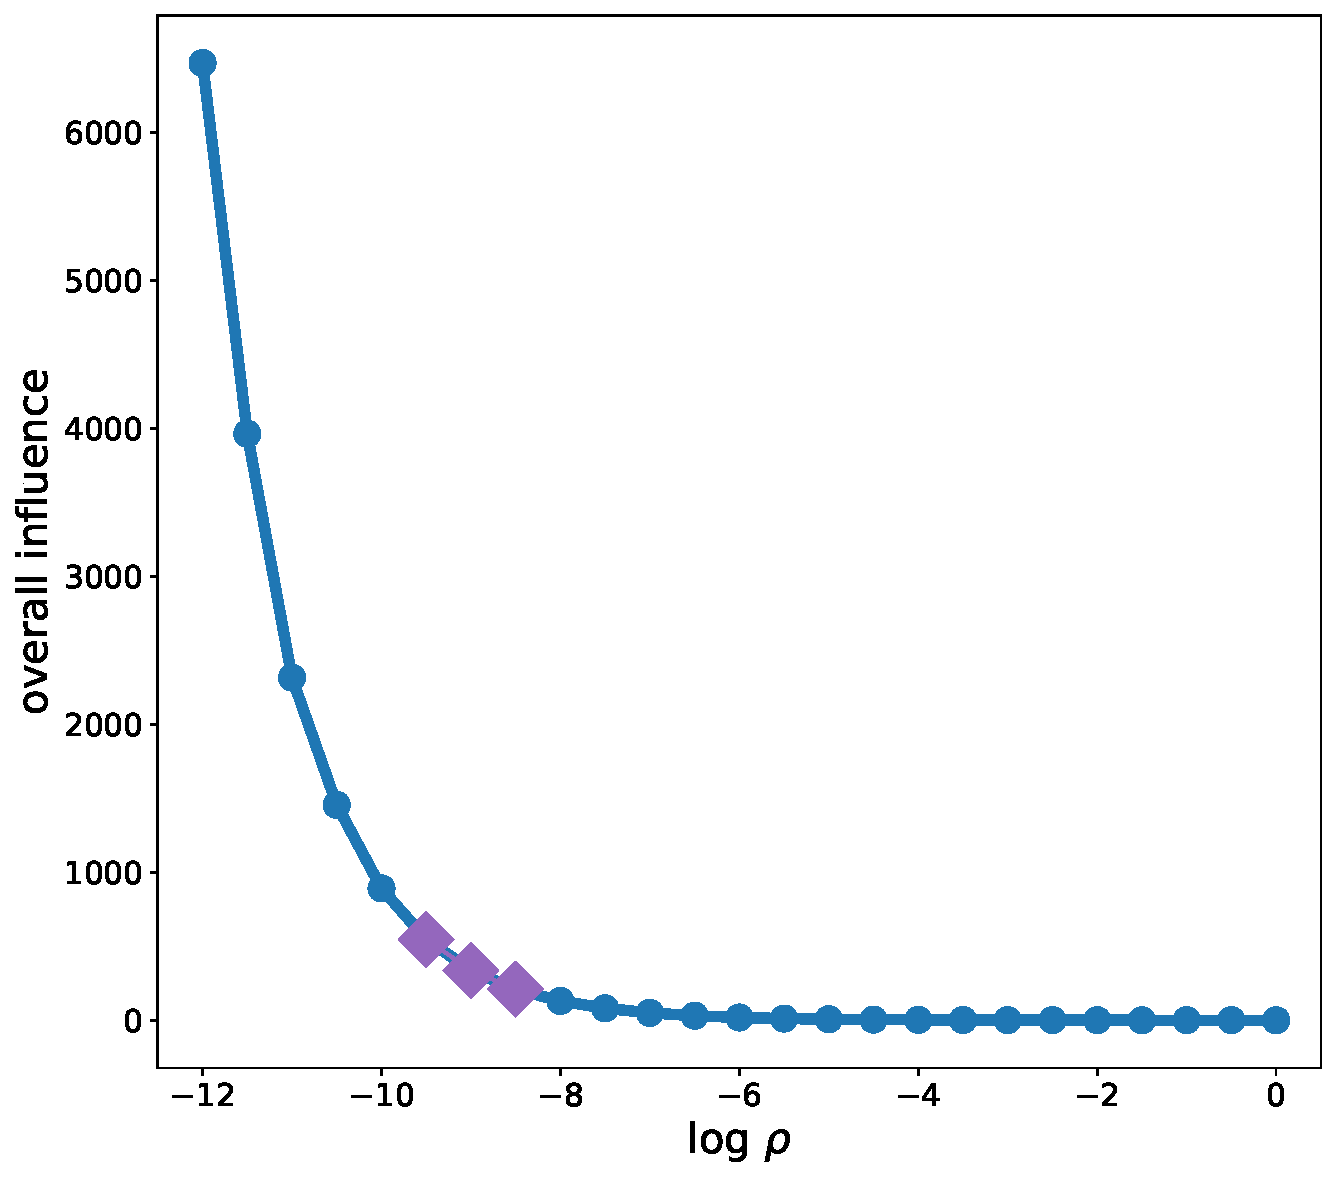
\includegraphics[width=0.7\textwidth]{../plots/waiting-SM-overall-empirical-influence-log-penalty-params-choose-best-baseden=Gamma-36-2-gridpoints=1-202-1.pdf}
%	\caption{XXXXX}
%	\label{fig-choose-appro-log-pen-param}
%\end{figure}
%
%In this plot, the points on the right end of the curve correspond to under-penalized SM density estimates that are very sensitive to the presence of $y$; and the the points on the left end of the curve correspond to over-penalized SM density estimates that are very insensitive to the presence of $y$. The points at the elbow corresponds to SM density estimates that are appropriately penalized. In this example, the points at the elbow (marked by purple diamonds) corresponds to $\rho = e^{-9.5}, e^{-9}$ and $e^{-8.5}$, and the corresponding penalized SM density estimates are shown in \textbf{\color{red}Figure \ref{XXXXXXX}}, which are all reasonable. 


\section{Which One to Use: Regularized Maximum Likelihood or Score Matching Density Estimators?}\label{section-which-one-to-use}

Now, we can compute penalized ML and regularized SM density estimators within $\calQ_{\ker}$. A natural question arises: which density estimator should one use? Regularized SM density estimators are easy to compute, and can be obtained by solving a linear system or adding and multiplying certain matrices, but are sensitive to the presence of isolated observations, especially when the amount of regularization is small. Penalized ML density estimator, on the other hand, is hard to compute as one has to handle $A$ and its derivative, but is \textit{not} very sensitive to the presence of isolated observations. We recommend to use regularized SM density estimators, primarily due to their computational advantage. When using them, one needs to impose an appropriate amount of regularization to ensure the resulting density estimate is not just a spike at the isolated observation or very close to the base density function $\mu$; otherwise, such a density estimate can be of no use and be misleading. One can use the $K$-fold cross-validation to select the appropriate amount of regularization as we did in this chapter and the earlier ones. % In terms of choosing between penalized and early stopping SM density estimators, we recommend the latter, again due to its computational advantage. 


\chapter{Summary and Future Directions}
\label{ch7}


\section{Summary}

In this dissertation, we focus on the density estimation problem in an exponential family induced by a RKHS, $\calQ_{\ker}$. We proposed a new early stopping SM density estimator obtained via minimizing the (unpenalized) SM loss functional by the gradient descent algorithm and terminating early. We studied its statistical properties and compared it with the penalized SM density estimator in the literature and showed their similarities and differences. 

We also compared these two kinds of regularized SM density estimators with the penalized ML density estimator. Via numerical examples, we observed that the regularized SM density estimators are very sensitive to the presence of an isolated observation, especially when there is a small amount of regularization, but the penalized ML density estimator does \emph{not}. We attempted to explain why this happens. 

In order to understand this phenomenon, we extended the classic notion of the influence function to allow its input to be a function-valued statistical functional. Using this extended influence function, we studied the sensitivity of regularized SM and ML density estimators in both finite-dimensional and kernel exponential families. 

As we have mentioned at the end of the preceding chapter, we recommend to use the regularized SM density estimators, mainly due to its computational advantages. But when using them, one needs to make sure an appropriate amount of regularization has been imposed. 

% In this report, we have focused on the density estimation problem in $\calQ_{\ker}$ and the comparison of penalized ML, penalized SM, and early stopping SM density estimators. We also extend the notion of the influence function to study the sensitivity of these density estimators. We found that, even though regularized SM density estimators are easy to be computed, they are very sensitive to the presence of isolated observations, especially when the regularization is small. Penalized ML density estimator is hard to be computed but is less sensitive to the presence of isolated observations. 

\section{Future Directions}

Numerical examples shown in this dissertation are restricted to $d = 1$. We conjecture that regularized SM density estimators in higher dimensions ($d \ge 2$) are also very sensitive to the presence of an isolated observation when the regularization is small, and need numerical examples to confirm this. 

% Recently, the SM loss functional has been used in studying Gaussian graphical models \parencite{Forbes2015-pe}. We do not expect the sensitivity issue discussed in the preceding section occurs to these models, as the canonical statistics in these models are not local basis functions. However, it is interesting to go beyond the Gaussian graphical models and see whether the applications of the SM loss functional result in sensitivity issues in other types of graphical models. 

Several versions of generalized SM loss functionals have been proposed in the literature in recent years. \textcite{Parry2012-pa} proposed a version that does not only involve the first two derivatives of a log-density function but also the higher-order derivatives. \textcite{Yu2020-fb} proposed the following generalized H-divergence between $p_0$ and $q$ 
\begin{align}\label{eq-yu-hdiv}
	\int_{\calX} p_0 \parens{x} \norm[\big]{\nabla \log p_0 \parens{x} \odot \sqrt{h \parens{x}} - \nabla \log q \parens{x} \odot \sqrt{h \parens{x}} }_2^2 \diff x, 
\end{align}
where $\odot$ denotes element-wise multiplication of two vectors, $h: \calX \to [0, \infty)^d$, and the square root is taken element-wise. Under certain regularity conditions, one can apply integration by parts and obtain a loss functional from \eqref{eq-yu-hdiv} that depends on $q$ only. It is interesting to apply these generalized SM loss functionals to the density estimation problem in $\calQ_{\ker}$ and see whether the resulting density estimators are sensitive to the presence of an isolated observation. We conjecture, with an appropriate choice of $h$ in \eqref{eq-yu-hdiv}, the resulting density estimators may \emph{not} be very sensitive to isolated observations. 

%As we have discussed in Chapter \ref{ch1}, there has been an increasing interest in log-concave density estimation recently. The dominant approach is to minimize the NLL loss functional over the class of log-concave density functions over $\Real^d$, resulting in the ML log-concave density estimator. This approach leads to a non-differentiable objective function to optimize and involves approximations of the normalizing constant and its sub-gradient, which is computationally challenging. In addition, as is shown in Figure \ref{fig-logconcave-mle}, the ML log-concave density estimates contain ridges, and are only supported over the convex hull of data with all boundary points being the discontinuous points of the density estimate, which are undesirable qualitative features and may cause series issues in statistical applications. 
%
%Since the SM loss functional does not involve the normalizing constant and involves the first two partial derivatives of the log-density function, it is interesting to estimate a log-concave density function by minimizing the SM loss functional and compare the resulting SM log-concave density estimator with the ML log-concave density estimator. We conjecture the issues with the ML log-concave density estimator described above can be solved by using the SM loss functional. 
%
%\begin{figure}
%	\centering
%	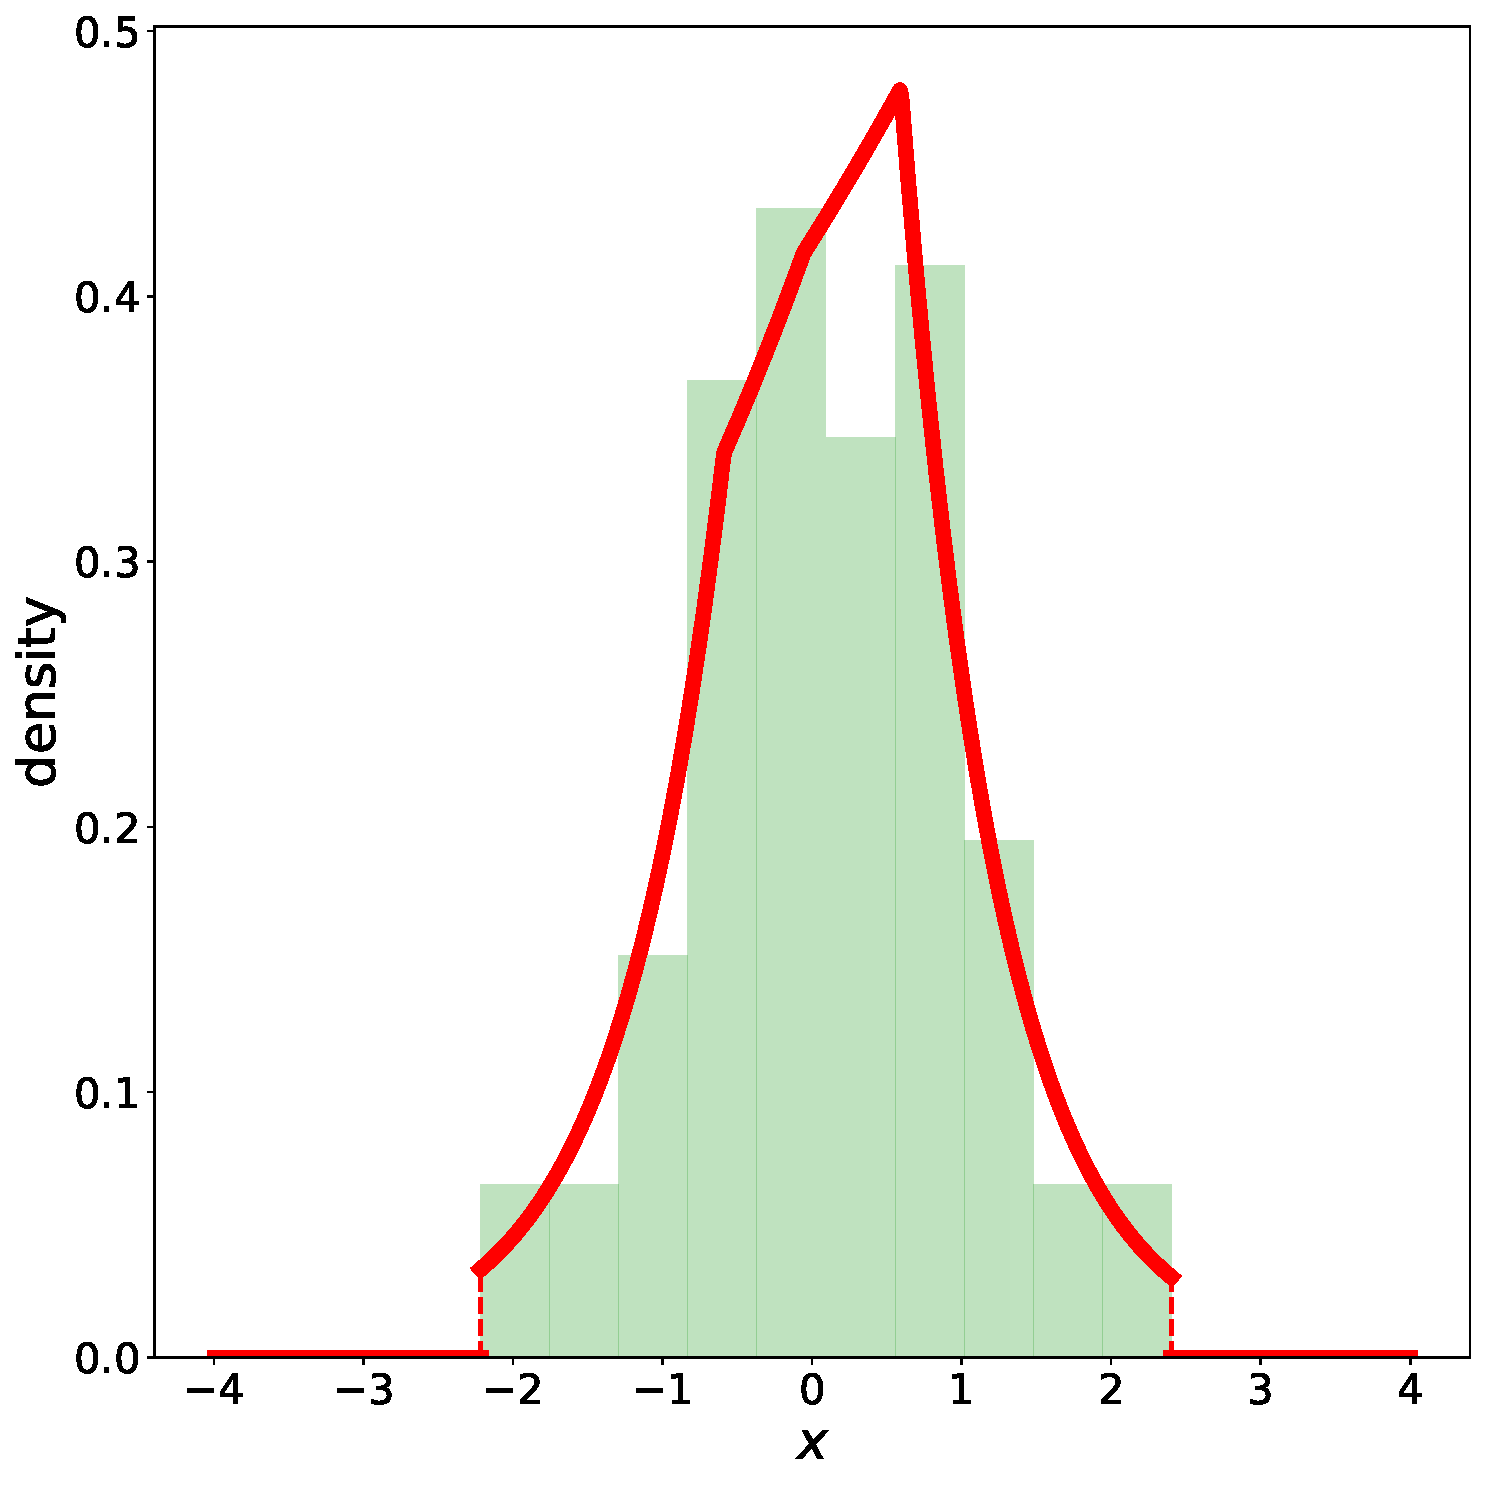
\includegraphics[width=0.6\textwidth]{../plots/log-concave-density-estimate-mle.pdf}
%	\caption{ML log-concave density estimate with 100 random samples from the standard normal distribution, where the density estimate is computed using the \texttt{R} package \texttt{logcondens} \parencite{Dumbgen2010-so}. Histogram with the bin width chosen by the Freedman-Diaconis rule is shown in green.}
%	\label{fig-logconcave-mle}
%\end{figure}



% If you have appendices in your dissertation, you will need the
% following, else keep it commented. The following appendices are in
% files called ``app1.tex'', and ``app2.tex'', and they
% look just like any chapter.
%

\appendix
\chapter{Math Background}
\label{app1}


\section{Fr{\'e}chet Differentiability and Derivative}\label{section-frechet-differentiable}

We provide details on the Fr{\'e}chet differentiability and derivative. Throughout this section, we let $\calH$ be a real Hilbert space, $J: \calH \to \Real$ be a map, $\calB \parens{\calH, \Real}$ denote the collection of all bounded linear operators from $\calH$ to $\Real$, and, similarly, $\calB \parens{\calH, \calH}$ denote the collection of all bounded linear operators from $\calH$ to itself. All materials of this section come from Section 2.6 in \textcite{Bauschke2017-he} and Section 5.1 in \textcite{Denkowski2013-ke}. 

\begin{definition}[Fr{\'e}chet differentiability and derivative]\label{def-frechet-differentiable}
	The map $J$ is said to be \textit{(first-order) Fr{\'e}chet differentiable} at $f \in \calH$ if there exists an operator $\Diff J \parens{f} \in \calB \parens{\calH, \Real}$ such that 
	\begin{align}\label{eq-frederivative}
	    \lim_{\substack{\norm{g}_{\calH} \to 0 \\ g \neq 0}} \frac{\abs[\big]{J \parens{f + g} - J \parens{f} - \Diff J \parens{f}\parens{g}}}{\norm{g}_{\calH}} = 0, 
	\end{align}
	and the operator $\Diff J \parens{f}$ is called the \textit{(first-order) Fr{\'e}chet derivative}. The map $J$ is said to be \textit{(first-order) Fr{\'e}chet differentiable on $\calH$} if it is Fr{\'e}chet differentiable at all $f \in \calH$. 
\end{definition}

\begin{proposition}
	Suppose $J$ is Fr{\'e}chet differentiable at $f \in \calH$ and the Fr{\'e}chet derivative $\Diff J \parens{f}$ exists. Then, $\Diff J \parens{f}$ is unique. 
\end{proposition}

\begin{remark}
	If $J$ is Fr{\'e}chet differentiable at $f \in \calH$, we then can write 
	\begin{align}\label{eq-frechet-derivative-interpretation}
		J \parens{f + g} = J \parens{f} + \Diff J \parens{f} \parens{g} + o \parens{\norm{g}_{\calH}}, 
	\end{align}
	for all $g \in \calH$ in a small neighborhood of the origin, where $o \parens{\norm{g}_{\calH}}$ denotes $\frac{o \parens{\norm{g}_{\calH}}}{\norm{g}_{\calH}} \to 0$ as $\norm{g}_{\calH} \to 0$. Thus, from \eqref{eq-frechet-derivative-interpretation}, we see $J \parens{f} + \Diff J \parens{f} \parens{g}$ provides the best linear approximation of $J$ in a small neighborhood of $f$, which is the similar interpretation of the derivative of a real-valued function of a single variable. 
\end{remark}

Frech{\'e}t derivative shares many properties of the derivative of a real-valued function of a single variable. The following proposition lists two properties we use in studying the Frech{\'e}t differentiability and deriving the Frech{\'e}t derivative of the log-partition functional $A$ in Chapter \ref{ch2}. 

\begin{proposition}\label{prop-property-frechet-differentiable}
\leavevmode
	\begin{enumerate}[label=(\alph*)]
		\item \label{prop-property-frechet-differentiable-a} Suppose $J_1, J_2: \calH \to \Real$ are Frech{\'e}t differentiable at $f \in \calH$ and $\alpha, \beta \in \Real$ are arbitrary. Then, $\alpha J_1 + \beta J_2$ is also Frech{\'e}t differentiable at $f \in \calH$, and 
		\begin{align*}
			\Diff \parens{\alpha J_1 + \beta J_2} \parens{f} = \alpha \Diff J_1 \parens{f} + \beta \Diff J_2 \parens{f}. 
		\end{align*}
		
		\item \label{prop-property-frechet-differentiable-b} (Chain rule) Suppose $J_1: \calH \to \Real$ is Frech{\'e}t differentiable at $f \in \calH$ and $J_2: \Real \to \Real$ is differentiable at $J_1 \parens{f}$. Then, $J_2 \circ J_1: \calH \to \Real$ is Frech{\'e}t differentiable at $f \in \calH$, and 
		\begin{align}
			\Diff \parens{J_2 \circ J_1} \parens{f} = J_2' \parens{J_1 \parens{f}} \Diff J_1 \parens{f}. 
		\end{align}
	\end{enumerate}
\end{proposition}

\begin{definition}[Fr{\'e}chet gradient]\label{def-frechet-gradient}
	Suppose $J: \calH \to \Real$ is Frech{\'e}t differentiable at $f \in \calH$. Since $\Diff J \parens{f}$ is a bounded linear map from $\calH$ to $\Real$, the Riesz-Fr{\'e}chet representation theorem \parencites[Fact 2.24 in][]{Bauschke2017-he} guarantees there exists a unique element $\nabla J \parens{f} \in \calH$ such that, for any $g \in \calH$, 
	\begin{align}\label{eq-frechet-grad}
		\Diff J \parens{f} \parens{g} = \innerp{g}{\nabla J \parens{f}}_{\calH}, 
	\end{align}
	and $\nabla J \parens{f}$ is called the \textit{Fr{\'e}chet gradient} of $J$ at $f$. If $J$ is Fr{\'e}chet differentiable on $\calH$, the \textit{Fr{\'e}chet gradient operator} is defined to be $\nabla J: \calH \to \calH, f \mapsto \nabla J \parens{f}$. 
\end{definition}

\begin{remark}
	Note that $\Diff J \parens{f}$ is a bounded linear map from $\calH$ to $\Real$, and belongs to the dual space of $\calH$, denoted by $\calH^*$. Since we have $\Diff J \parens{f} \parens{g} = \innerp{\nabla J \parens{f}}{g}_{\calH}$, the Riesz-Fr{\'e}chet representation theorem implies that $\norm{\Diff J \parens{f}}_{\calH^*} = \norm{\nabla J \parens{f}}_{\calH}$, where $\norm{}_{\calH^*}$ denotes the norm of the dual space $\calH^*$. 
\end{remark}

We now extend Definition \ref{def-frechet-differentiable} to higher orders. 

\begin{definition}[Higher-order Fr{\'e}chet differentiability and derivatives]\label{def-frechet-derivative-higher-order}
	Higher-order Fr{\'e}chet differentiability and derivatives are defined inductively. 
	
	In particular, the map $J$ is said to be \textit{twice Fr{\'e}chet differentiable at $f \in \calH$} if $J$ itself is Fr{\'e}chet differentiable at $f \in \calH$ and the map $\Diff J \parens{f}: \calH \to \Real$ is also Fr{\'e}chet differentiable at $f \in \calH$. The \textit{second Fr{\'e}chet derivative} of $J$ at $f \in \calH$, denoted by $\Diff^2 J \parens{f}$, is an operator from $\calH$ to $\calB \parens{\calH, \Real}$, that satisfies 
	\begin{align}\label{eq-2ndfrederivative}
		\lim_{\substack{\norm{g}_{\calH} \to 0 \\ g \neq 0}} \frac{\norm[\big]{\Diff J \parens{f + g} - \Diff J \parens{f} - \Diff^2 J \parens{f} \parens{g} }_{\calH^*}}{\norm{g}_{\calH}} = 0, 
	\end{align}
	where $\norm{\,\cdot\,}_{\calH^*}$ denotes the norm of the dual space of $\calH$. The map $J$ is said to be \textit{twice Fr{\'e}chet differentiable on $\calH$} if it is twice Fr{\'e}chet differentiable at all $f \in \calH$. 
	
	Suppose $J$ is twice Fr{\'e}chet differentiable on $\calH$. The \textit{second-order Fr{\'e}chet gradient operator}, denoted by $\nabla^2 J$, is a bounded linear operator that maps from $\calH$ to $\calB \parens{\calH, \calH}$ and satisfies 
	\begin{align*}
		\Diff^2 J \parens{f} \parens{g} \parens{h} = \innerp{h}{ \nabla^2 J \parens{f} \parens{g}}_{\calH}, \qquad \text{ for all } f, g, h \in \calH. 
	\end{align*}
	In other words, $\nabla^2 J \in \calB \parens{\calH, \calB \parens{\calH, \calH}}$ and $\nabla^2 J \parens{f} \in \calB \parens{\calH, \calH}$ for all $f \in \calH$. 
\end{definition}

%\begin{remark}
%	By Proposition 5.1.17 in \textcite{Denkowski2013-ke}, there exists an isometric isomorphism between $\calB \parens{\calH, \calB \parens{\calH, \calH}}$ and $\calB \parens{\calH \times \calH, \calH}$. Let $\Phi$ denote this isometric isomorphism. Then, $\Phi \parens{\nabla^2 J}$ is a map from $\calH \times \calH$ to $\calH$ such that $\Phi \parens{\nabla^2 J} \parens{f, \, g} = \nabla^2 J \parens{f} \parens{g}$, for all $f, g \in \calH$. 
%\end{remark}


\section{Bochner Integral}\label{section-bochner-integral}

In this section, we present the definition of the Bochner integral, which is the extension of the Lebesgue integral of real-valued functions to the integral of functions taking values in a Banach space. We also present some properties of the Bochner integral that we have used in the dissertation (in particular, in Chapter \ref{ch2} and \ref{ch3}). All materials of this section come from Appendix A.5.3 in \textcite{Steinwart2008-tn} and Section 3.10 \textcite{Denkowski2013-ke}. 

Throughout this section, let $\calE$ be a Banach space whose norm is denoted by $\norm{}_{\calE}$, and $\parens{\calX, \Sigma, \mu}$ be a $\sigma$-finite measure space (note that this $\mu$ differs from the one in the definition of finite-dimensional and kernel exponential families in Chapter \ref{ch2}). We first define the simple function (Definition \ref{def-simple-fun}) and the measurable function (Definition \ref{def-measurable-fun}) in the Banach space setting  and then define the Bochner $\mu$-integral (Definition \ref{def-bochner-integral}). 

\begin{definition}[$\calE$-valued simple function]\label{def-simple-fun}
	A function $s: \calX \to \calE$ is said to be an \textit{$\calE$-valued simple function} if there exist $e_1, \cdots, e_n \in \calE$ and $A_1, \cdots, A_n \in \Sigma$ such that 
	\begin{align*}
		s \parens{x} = \sum_{i=1}^n \indic_{A_i} \parens{x} e_i, \qquad \text{ for all } x \in \calX, 
	\end{align*}
	where $\indic_A$ is the indicator function of the set $A$, and is equal to 1 if $x \in A$ and to 0, otherwise. 
\end{definition}

\begin{definition}[$\calE$-valued measurable function]\label{def-measurable-fun}
	A function $f: \calX \to \calE$ is said to be an \textit{$\calE$-valued measurable function} if there exists a sequence of $\calE$-valued simple functions, $\sets{s_n}_{n \in \Natural}$, such that
	\begin{align}
		\lim_{n \to \infty} \norm{f \parens{x} - s_n \parens{x}}_{\calE} = 0
	\end{align}
	holds for all $x \in \calX$. 
\end{definition}

\begin{definition}[Bochner $\mu$-integral]\label{def-bochner-integral}
	An $\calE$-valued measurable function $f: \calX \to \calE$ is said to be \textit{Bochner $\mu$-integrable} if there exists a sequence of $\calE$-valued simple functions, $\sets{s_n}_{n \in \Natural}$, such that
	\begin{align}
		\lim_{n \to \infty} \int_{\calX} \norm{s_n \parens{x} - f \parens{x}}_{\calE} \ \diff \mu \parens{x} = 0. 
	\end{align}
	In this case, the limit
	\begin{align*}
		\int_{\calX} f \parens{x} \diff \mu \parens{x} := \lim_{n \to \infty} \int_{\calX} s_n \parens{x} \diff \mu \parens{x}
	\end{align*}
	exists and is called the \textit{Bochner $\mu$-integral} of $f$. 
\end{definition}

A criterion to check the Bochner $\mu$-integrability is the following. 

\begin{proposition}\label{prop-bochner-integrability}
	A measurable function $f: \calX \to \calE$ is Bochner $\mu$-integrable if and only if $\int_{\calX} \norm{f \parens{x}}_{\calE} \diff \mu \parens{x} < \infty$. 
\end{proposition}

Finally, we look at some properties of Bochner $\mu$-integral we use. 

\begin{proposition}\label{prop-properties-bochcher-integral}
	The Bochner $\mu$-integral defined above has the following properties: 
	\begin{enumerate}[label=(\alph*)]
		\item \label{prop-properties-bochcher-integral-a} The Bochner $\mu$-integral is linear. 
		\item \label{prop-properties-bochcher-integral-b} If $f: \calX \to \calE$ is Bochner $\mu$-integrable, we have 
		\begin{align*}
			\norm[\bigg]{\int_{\calX} f \parens{x} \diff \mu \parens{x}}_{\calE} \le \int_{\calX} \norm{f \parens{x}}_{\calE} \diff \mu \parens{x}. 
		\end{align*}
		\item \label{prop-properties-bochcher-integral-c} Suppose $\calE'$ is another Banach space. If $S: \calE \to \calE'$ is a bounded linear operator and $f: \calX \to \calE$ is Bochner $\mu$-integrable, then $S \circ f: \calX \to \calE'$ is also Bochner $\mu$-integrable. In this case, the integral commutes with $S$, that is, 
		\begin{align*}
			S \parens[\bigg]{\int_{\calX} f \parens{x} \diff \mu \parens{x}} = \int_{\calX} \parens{S \circ f} \parens{x} \, \diff \mu \parens{x}. 
		\end{align*}
	\end{enumerate}
\end{proposition}


\section{Partial Derivatives of a Kernel Function}\label{section-kernel-derivative}

In this section, we discuss the partial derivatives of the kernel function associated with a RKHS and their reproducing property. We follow the development in Section 4.3 in \textcite{Steinwart2008-tn} and the paper by \textcite{Zhou2008-jt}. Throughout this section, we let $\calX \subseteq \Real^d$ be an open set and $\Natural_0 := \Natural \cup \sets{0}$. 

We first consider a real-valued function $f: \calX \to \Real$. The function $f$ is said to be \textit{$m$-times continuously differentiable} if, for all $\alpha := \parens{\alpha_1, \cdots, \alpha_d}^\top \in \Natural_0^d$ with $\abs{\alpha} := \sum_{i=1}^d \alpha_i \le m$ and all $x \in \calX$, 
\begin{align*}
	\partial^\alpha f \parens{x} 
	%= \partial_1^{\alpha_1} \cdots \partial_d^{\alpha_d} f \parens{x} 
	= \frac{\partial^{\abs{\alpha}}}{\partial u_1^{\alpha_1} \cdots \partial u_d^{\alpha_d}} f \parens{u} \bigg\vert_{u=x}, 
\end{align*}
exists, where $u := \parens{u_1, \cdots, u_d}^\top \in \calX$. 

%\begin{lemma}[Differentiability of feature maps (Lemma 4.34 in \cite{Steinwart2008-tn})]\label{derivative.reproducing}
%	Let $\calX \subseteq \Real^d$ be an \textit{open} subset, $k$ be a kernel on $\calX$, $\calH$ be the RKHS of $k$, and $\Phi: \calX \to \calH$ be a feature map of $k$. Let $i \in \sets{1, \cdots, d}$ be an index such that the mixed partial derivative $\partial_i \partial_{i+d} k$ of $k$ with respect to the coordinates $i$ and $i+d$ exists and is continuous, where. Then the partial derivative $\partial_i \Phi$ of $\Phi: \calX \to \hil$ with respect to the $i$-th coordinate exists, is continuous, and for all $x, x \in \calX$, we have
%	\begin{align}
%		\innerp{\partial_i \Phi \parens{x}}{\partial_{i} \Phi \parens{x'}}_{\calH} = \partial_i \partial_{i+d} k \parens{x, x'} = \partial_{i+d} \partial_i k \parens{x, x'}. 
%	\end{align}
%\end{lemma}

We then define the $m$-times continuous differentiability of the kernel function $k$. 

\begin{definition}[$m$-times continuous differentiability of a kernel function]
	Let $k: \calX \times \calX \to \Real$ be a kernel function and $m \in \Natural$. We say $k$ is \textit{$m$-times continuously differentiable} if $\partial^{\alpha, \alpha}k: \calX \times \calX \to \Real$ exists and is continuous for all $\alpha := \parens{\alpha_1, \cdots, \alpha_d} \in \Natural_0^d$ with $\abs{\alpha} := \sum_{i=1}^d \alpha_i \le m$, where 
	\begin{align*}
		\partial^{\alpha, \alpha} k \parens{x, y} 
		%= \partial_1^{\alpha_1} \cdots \partial_d^{\alpha_d} \partial_{1+d}^{\alpha_1} \cdots \partial_{2d}^{\alpha_d} k \parens{x, y} 
		= \frac{\partial^{2\abs{\alpha}}}{\partial u_1^{\alpha_1} \cdots \partial u_d^{\alpha_d} \partial v_1^{\alpha_1} \cdots \partial v_d^{\alpha_d}} k \parens{u, v}\bigg\vert_{u=x, v=y}, \qquad \text{ for all } x, y \in \calX. 
	\end{align*}
\end{definition}

%\begin{remark}
%	\begin{enumerate}
%	\item From the lemma above, it is observed that $\partial_i \partial_{i+d} k$ is a kernel on $\calX \times \calX$ with the feature map $\partial_i \Phi$. 
%	\item Assuming that $\partial_i \partial_{i+d} \partial_j \partial_{j+d} k$ exists and is continuous, applying the lemma above iteratively one can show that $\partial_j \partial_i \Phi$ exists, is continuous, and is a feature map of the kernel $\partial_i \partial_{i+d} \partial_j \partial_{j+d} k$. 
%	\end{enumerate}
%\end{remark}

The partial derivative of $k$ is an element in $\calH$ and has the reproducing property as $k$ does, as the following proposition states. 

\begin{proposition}[Partial derivatives of kernels and its reproducing property]\label{prop-reproducing-derivative}
	Let $\calH$ be a RKHS with the kernel function $k: \calX \times \calX \to \Real$, and assume $k$ is $m$-times continuously differentiable on $\calX$. Then, 
	\begin{enumerate}[label=(\alph*)]
		\item we have 
		\begin{align}
			\partial^{\alpha} k \parens{x, \,\cdot\,} 
			%= \partial_1^{\alpha_1} \cdots \partial_d^{\alpha_d} k \parens{x, \,\cdot\,} 
			= \frac{\partial^{\abs{\alpha}}}{\partial u_1^{\alpha_1} \cdots \partial u_d^{\alpha_d}} k \parens{u, \,\cdot\,}\bigg\vert_{u=x} \in \calH
		\end{align}
		where $u := \parens{u_1, \cdots, u_d}^\top \in \calX$, and 
		\item every $f \in \hil$ is $m$-times continuously differentiable, and, for all $\alpha \in \Natural_0^d$ with $\abs{\alpha} \le m$ and all $x \in \calX$, the partial derivative reproducing property holds, i.e., 
		\begin{align}
			\partial^{\alpha} f \parens{x} = \innerp{\partial^{\alpha} k \parens{x, \,\cdot\,}}{f}_{\calH}, \qquad \text{ for all } x \in \calX. %, \hspace{20pt} \text{and}\hspace{20pt}  \abs{\partial^{\alpha} f(x)} \le \norm{f}_{\hil} \cdot \sqrt{\partial^{\alpha, \alpha} k\pare{x, x}}. 
		\end{align}
		In particular, we have $\partial^{\alpha, \alpha} k \parens{x, y} = \innerp{\partial^{\alpha} k \parens{x, \,\cdot\,}}{\partial^{\alpha} k \parens{y,\,\cdot\,}}_{\calH}$ for all $x, y \in \calX$. 
	\end{enumerate}
\end{proposition}


\section{Some Theories on Bounded Linear Operators}\label{section-bdd-linear-operator}

In our development in Chapters \ref{ch2} and \ref{ch3}, we have used some theories on the bounded linear operators in a Hilbert space. In this section, we aim to give a very brief overview of these theories. More information can be found in, for example, Chapters 13 and 16 in \textcite{Royden2018-cd} and Chapter VI in \textcite{Reed2012-xs}. 

Throughout this section, we let $\calH$ be a real Hilbert space with the inner product $\innerp{\,\cdot\,}{\,\cdot\,}_{\calH}$ and the norm $\norm{}_{\calH}$, and assume $\calH$ is separable, meaning that it contains a dense countable subset. Due to the separability of $\calH$, it admits a countable orthonormal basis. 

\begin{definition}[Linear operator]
	An operator $C: \calH \to \calH$ is said to be \textit{linear} if, for any $f, g \in \calH$ and any $\alpha, \beta \in \Real$, we have 
	\begin{align*}
		C \parens{\alpha f + \beta g} = \alpha C f + \beta C g. 
	\end{align*}
\end{definition}

\begin{definition}[Bounded operator]
	A linear operator $C: \calH \to \calH$ is said to be \textit{bounded} if there exists a constant $M \ge 0$ such that 
	\begin{align*}
		\norm{C f}_{\calH} \le M \cdot \norm{f}_{\calH}, \qquad \text{ for all } f \in \calH. 
	\end{align*}
	The infimum of all such $M$ is called the \textit{operator norm} of $C$ and is denoted by $\norm{C}$. 
\end{definition}

\begin{definition}[Adjoint and self-adjoint operators]
	Let $C: \calH \to \calH$ be a bounded linear operator. Then, the \textit{adjoint} of $C$ is the bounded linear operator $C^*: \calH \to \calH$ satisfying 
	\begin{align*}
		\innerp{Cf}{g}_{\calH} = \innerp{f}{C^*g}_{\calH}, \qquad \text{ for all } f, g \in \calH. 
	\end{align*}
	The adjoint $C^*$ exists and is unique. 
	
	The operator $C$ is said to be \textit{self-adjoint}, if $C = C^*$, that is, $\innerp{Cf}{g}_{\calH} = \innerp{f}{Cg}_{\calH}$ for all $f, g \in \calH$. 
\end{definition}

\begin{definition}[Positive semidefinite and definite operators]
	Let $C: \calH \to \calH$ be a self-adjoint bounded linear operator. Then, $C$ is said to be \textit{positive semidefinite} if, for all $f \in \calH$, $\innerp{f}{Cf}_{\calH} \ge 0$, and to be \textit{positive definite} if, for all $f \in \calH \backslash \sets{0}$, $\innerp{f}{Cf}_{\calH} > 0$. 
\end{definition}

\begin{definition}[Compact operator]
	A bounded linear operator $C: \calH \to \calH$ is said to be \textit{compact}, if, for every bounded sequence $\sets{f_n}_{n \in \Natural}$ in $\calH$, $\sets{C f_n}_{n \in \Natural}$ has a subsequence that converges in $\calH$ (with respect to the norm $\norm{}_{\calH}$). 
\end{definition}

Other equivalent ways of defining a compact operator can be found, for example, in Section 16.5 in \textcite{Royden2018-cd} and Section VI.5 in \textcite{Reed2012-xs}. 

\begin{definition}[Finite rank operator]
	A bounded linear operator $C: \calH \to \calH$ is said to be of \textit{finite rank} if its range is finite-dimensional. That is, every element in $\range \parens{C}$ can be written as $Cf = \sum_{i=1}^m \alpha_i g_i$, for some $f \in \calH$, some fixed family $\sets{g_i}_{i=1}^m \subset \calH$, some $\alpha_1, \cdots, \alpha_m \in \Real$, and $m < \infty$. 
\end{definition}

The relationship between the compact operator and the finite rank operator is given in the following proposition. 

\begin{proposition}
	Every finite rank operator is compact. In addition, every compact operator on $\calH$ is the norm limit of a sequence of finite rank operators. 
\end{proposition}

In addition, we have the following characterization when the identity operator is compact. 

\begin{proposition}
	The identity operator $I: \calH \to \calH$ is compact if and only if $\calH$ is finite-dimensional. 
\end{proposition}

We also have the following result characterizing the relationship between the invertibility and the compactness of a bounded linear operator. 

\begin{proposition}\label{prop-invertible-compact-infdim}
	Let $\calH$ be infinite-dimensional and $C: \calH \to \calH$ be a bounded linear operator. If $C$ is compact, it is \emph{not} invertible. 
\end{proposition}

In the development in Chapter \ref{ch3}, we have repeatedly used the following Hilbert-Schmidt theorem, which is an extension of the eigen-decomposition of a real symmetric matrix. 

\begin{theorem}[Hilbert-Schmidt theorem]\label{theorem-hilbert-schmidt}
	Let $C: \calH \to \calH$ be a self-adjoint compact operator. There exists an orthonormal basis $\sets{\psi_{\nu}}_{\nu=1}^R$ for $\overline{\range \parens{C}}$, together with a monotonically non-increasing sequence of nonzero real numbers $\sets{\xi_{\nu}}_{\nu=1}^R$, such that $C \psi_{\nu} = \xi_{\nu} \psi_{\nu}$ for all $\nu = 1, \cdots, R$. In addition, the following identity holds 
	\begin{align*}
		C f = \sum_{\nu=1}^R \xi_{\nu} \innerp{f}{\psi_{\nu}}_{\calH} \psi_{\nu}, \qquad \text{ for all } f \in \calH. 
	\end{align*}
	If $C$ is of finite rank, then $R < \infty$ and $R$ is the rank of $C$; if $C$ is not of finite rank, $R = \infty$ and $\lim_{\nu \to \infty} \xi_{\nu} = 0$. 
\end{theorem}

In Theorem \ref{theorem-hilbert-schmidt}, the functions $\psi_{1}, \cdots, \psi_{R}$ are called the \textit{eigenfunctions} of $C$, and $\xi_{\nu}$ is called the \textit{eigenvalue} of $C$ associated with the eigenfunction $\psi_{\nu}$, for all $\nu = 1, \cdots, R$. 

Using Theorem \ref{theorem-hilbert-schmidt}, it is easy to see that, if $C$ is positive semidefinite, all its eigenvalues are positive. 

We next introduce two special classes of bounded linear operators, the trace class and the Hilbert-Schmidt class, that are of great importance in proving various properties of penalized and early stopping SM density estimators in Chapter \ref{ch2} and \ref{ch3}. 

We first introduce the trace of a bounded linear operator, based on which we define the trace class. 

\begin{definition}[Trace]
	Let $\sets{\psi_{\nu}}_{\nu=1}^{\infty}$ be an orthonormal basis of $\calH$. For any positive definite bounded linear operator $C: \calH \to \calH$, the \textit{trace} of $C$ is defined to be 
	\begin{align*}
		\trace \parens{C} := \sum_{\nu=1}^{\infty} \innerp{\psi_{\nu}}{C \psi_{\nu}}_{\calH}, 
	\end{align*}
	where the sum is independent of the choice of the orthonormal basis. 
\end{definition}

\begin{definition}[Trace class]
	A bounded linear operator $C: \calH \to \calH$ is said to be of \textit{trace class} if $\tr \parens{\abs{C}} < \infty$. 
\end{definition}

Then, we have the following properties of operators that are of trace class. 

\begin{proposition}
	Let $C: \calH \to \calH$ be of trace class. Then, $C$ is compact, and its operator norm, $\norm{C}$, and its trace, $\tr \parens{C}$, are related by $\norm{C} \le \tr \parens{C}$. 
\end{proposition}

We now turn to the Hilbert-Schmidt operator. 

\begin{definition}[Hilbert-Schmidt operator]
	Let $\sets{\psi_{\nu}}_{\nu=1}^{\infty}$ be an orthonormal basis of $\calH$. A bounded linear operator $C: \hil \to \hil$ is said to be \textit{Hilbert-Schmidt (HS)} if 
	\begin{align*}
		\sum_{\nu=1}^{\infty} \norm{C \psi_{\nu}}^2_{\calH} < \infty. 
	\end{align*}
\end{definition}

Still let $\sets{\psi_{\nu}}_{\nu=1}^{\infty}$ be an orthonormal basis of $\calH$. Given two HS operators $C_1, C_2: \hil \to \hil$, define the \textit{HS inner product} between them to be 
\begin{align*}
	\innerp{C_1}{C_2}_{\mathrm{HS}} = \sum_{\nu=1}^{\infty} \innerp{C_1 \psi_{\nu}}{C_2 \psi_{\nu}}_{\hil}, 
\end{align*}
and the \textit{HS norm} to be 
\begin{align*}
	\norm{C_1}_{\mathrm{HS}} := \sqrt{\innerp{C_1}{C_1}_{\mathrm{HS}}} = \sqrt{\tr \parens{C_1^* C_1}} = \parens[\Bigg]{\sum_{\nu=1}^{\infty} \norm{C_1 \psi_{\nu}}^2_{\hil}}^{1/2}. 
\end{align*}

We then have the following properties of HS operators. 

\begin{proposition}[Properties of HS operators]\label{prop-hs-property}
	The following properties of the HS operators hold: 
	\begin{enumerate}[label=(\alph*)]
		\item \label{prop-hs-property-a} Let $C: \hil \to \hil$ be a HS operator. Then, its operator norm $\norm{C}$, its trace $\trace \parens{C}$, and its HS norm $\norm{C}_{\mathrm{HS}}$ are related by $\norm{C} \le \norm{C}_{\mathrm{HS}} \le \trace \parens{C}$. 
		\item \label{prop-hs-property-b} The class of all HS operators with the inner product $\innerp{\,\cdot\,}{\,\cdot\,}_{\mathrm{HS}}$ forms a Hilbert space. 
		\item \label{prop-hs-property-c} Every HS operator is compact. 
	\end{enumerate}
\end{proposition}


% \include{app2}


% The all important bibliography file at the end of your document!! Use
% the bibstyle you (your department) like in the \bibliographystyle{}
% statement and list the name of your bibliography database file in
% the \bibliography{} statement.  In this example, ``bibfile.bib'' is
% the name of the database.  See the LaTeX manual appendix B for details
% about the bibliography database and BibTeX.
%


\begingroup
\setstretch{2.0}
\printbibliography
\endgroup


\end{document}

